\documentclass[12pt]{report}

%%
% to enumerate subsubsection
%%
\addtocounter{tocdepth}{3}
\setcounter{secnumdepth}{3}
% \usepackage{tgtermes}
\usepackage[a4paper, margin=1in]{geometry}
\usepackage[T1]{fontenc}
\usepackage[utf8]{inputenc}
\usepackage{graphicx} 
\usepackage{tikz}
\usepackage{amsmath, amssymb}
% \usepackage{indentfirst}
% \usepackage{cite}
\usepackage{natbib}
\usepackage[nameinlink,noabbrev]{cleveref}
\usepackage[capposition=top]{floatrow}
\usepackage{float}
\usepackage{caption}
\usepackage{xfrac}
\usepackage{braket}
\usepackage[toc,page]{appendix}
\usepackage{tabularx}
% \usepackage{hyperref}

%%
% to enumerate subsubsection
%%
\addtocounter{tocdepth}{3}
\setcounter{secnumdepth}{3}

% Snippet
\newcommand{\BSM}{Black--Scholes--Merton }
\newcommand{\lnorm}{log-normally }
\newcommand{\bmotion}{Brownian Motion }
\newcommand{\stvar}{stochastic variable }
\newcommand{\wienpro}{Wiener process }
\newcommand{\markpro}{Markov process }

% 
% Bunch of new commands
% 
% brownian motion
\newcommand{\dBm}{dW\left(t\right)}
\newcommand{\dpoiss}{dq\left(t\right)}
\newcommand{\DBm}{\delta{W\left(t\right)}}
\newcommand{\Bm}{W\left(t\right)}
\newcommand{\Bmsub}[1]{W_{#1}\left(t\right)}
\newcommand{\Dt}{\Delta t} 
\newcommand{\Bmdist}{\DBm \sim N \left( 0, \Dt \right)}
\newcommand{\ft}{f\left(t, \Bm \right)}
\newcommand{\E}{\mathop{\mathbb{E}}}
\newcommand{\ct}{c\left(t, x\right)}
\newcommand{\dcx}{\frac{\delta\ct}{\delta x}}
\newcommand{\dciix}{\frac{\delta^2\ct}{\delta x^2}}
\newcommand{\dct}{\frac{\delta\ct}{\delta t}}
\newcommand{\N}[1]{N\left(#1\right)}
\newcommand{\dsub}[1]{d_{#1}\left(\Dt, x\right)}
\newcommand{\call}[2]{c\left( #1, #2\right)}
% % about stock
\newcommand{\St}{S\left(t\right)}
\newcommand{\Vt}{V\left(t\right)}
\newcommand{\Si}{S\left(0\right)}
\newcommand{\dSt}{dS\left(t\right)}
\newcommand{\DSt}{\Delta S\left(t\right)}
\newcommand{\dSr}{\frac{\dSt}{\St}}
\newcommand{\DSr}{\frac{\DSt}{\St}}
\newcommand{\Scontinuous}{\St = \Si e^{\sigma\Bm + \left(\alpha - \frac{1}{2 \sigma^2}\right)t}}
\newcommand{\Itobmdiff}{d\ft = \left[\frac{\partial \ft }{\partial t} + \frac{1}{2} \frac{\partial ^2\ft }{\partial x^2}\right]dt + \frac{\partial \ft}{\partial x} \dBm}
\newcommand{\Scontinousdiff}{d\St &= \alpha \St dt + \sigma \St \dBm}
\newcommand{\Scontinuousrate}{\dSr &= \alpha dt + \sigma \dBm}
 \newcommand{\Sdiscretediff}{d\St &= \alpha \St \Dt + \sigma \St \dBm}
\newcommand{\Sshort}{\Si e^{X}}
\newcommand{\CCRdist}{X \sim N\left(\left(\alpha - \frac{1}{2}\sigma^2\right)t, \sigma^2 t\right)}
\newcommand{\Sdiscreterate}{\DSr &= \alpha \Delta t + \sigma \DBm}
\newcommand{\Sdiscreterateexp}{\E \DSr = \alpha \Dt}
\newcommand{\Sdiscreteratevar}{var \DSr = \sigma ^2 \Dt}
\newcommand{\Sdiscreteratedist}{\DSr \sim N\left(\alpha\Dt, \sigma\Dt\right)}
\newcommand{\Sexp}{\E\St = \Si e^{\alpha t}}
\newcommand{\Svar}{var\St = \Si^2 e^{2\alpha t}\left(e^{\sigma^2 t} - 1\right)}
\newcommand{\Sshortt}{\St = \Si e^{X t}}
\newcommand{\CCRt}{X = \frac{1}{t} \ln{\frac{\St}{\Si}}}
\newcommand{\CCRtdist}{X \sim N\left(\alpha - \frac{\sigma^2}{2}, \frac{\sigma^2}{t}\right)}
\newcommand{\BSMpde}{\dct + r x \dcx + \frac{1}{2} \sigma^2 x^2 \dciix = r\ct}
\newcommand{\BSMeq}[1]{r\call{t}{#1} = \frac{\partial \call{t}{#1}}{\partial t} + r #1 \frac{\partial \call{t}{#1}}{\partial #1} + \frac{1}{2} \sigma ^2 #1 ^2 \frac{\partial ^2 \call{t}{#1}}{\partial #1 ^2}}
\newcommand{\BSMGreeks}[1]{r\call{t}{#1} = \Theta + r #1 \Delta + \frac{1}{2} \sigma ^2 #1 ^2 \Gamma}
\newcommand{\BSMsol}{\ct &= x\N{\dsub{+}} - K e^{-r\Dt} \N{\dsub{-}}}
\newcommand{\dpm}{\dsub{\pm} &= \frac{1}{\sigma\sqrt{\Dt}} \left[\log\frac{x}{K} + \left(r \pm \frac{\sigma^2}{2}\Dt\right)\right]}

% CIR Stock price Stochastic process
\newcommand{\HSVstock}{
  d\St &= \alpha \St dt + \sqrt{\Vt} \St d \Bmsub{S}
}

% CIR Stock price Stochastic process
\newcommand{\HSVstockriskless}{
  d\St &= r \St dt + \sqrt{\Vt} \St d \Bmsub{S}
}

% CIR volatility
\newcommand{\HSVvol}{
  d\Vt &= \kappa\left(\theta - \Vt \right) dt + \sigma \sqrt{\Vt} d \Bmsub{V}
}


% CIR volatility
\newcommand{\HSVvolriskless}{
  d\Vt &= \kappa^{*} \left(\theta^{*} - \Vt \right) dt + \sigma \sqrt{\Vt} d \Bmsub{V}
}

\newcommand{\dportfolio}{dX\left(t\right) &= \Delta\left(t\right) d\St + r \left(X\left(t\right) - \Delta\left(t\right) \St \right) dt}

\usepackage{Sweave}
\begin{document}
\Sconcordance{concordance:index.tex:index.Rnw:%
1 18 1 1 0 13 1}
\Sconcordance{concordance:index.tex:./State/index.Rnw:ofs 33:%
1 55 1}
\Sconcordance{concordance:index.tex:index.Rnw:ofs 89:%
34 4 1}

\tableofcontents{}



%%%%%%%%%%%%%%%%%%%%%%%%%%%%%%%%%%%%%%%%%%%%%%%%%%%%%%%%%%%%%%%%%%%%%%%%%%%%%%%%
%
%  CHAPTER: Introduction
%
%%%%%%%%%%%%%%%%%%%%%%%%%%%%%%%%%%%%%%%%%%%%%%%%%%%%%%%%%%%%%%%%%%%%%%%%%%%%%%%%
\chapter*{Introduction}
\label{cha:Introduction}
\addcontentsline{toc}{chapter}{Introduction}

Talk about what is done to price a vanilla option throuhout the BSM method.
How does the BSM model is fair under its assumption. What about if we are going beyond ?
How perfomant is it ? 
What about other model such as \ldots ?

Using R. \cite{R}
% \SweaveInput{upstream}
% \SweaveInput{underlying}
% \SweaveInput{BSM}
%%%%%%%%%%%%%%%%%%%%%%%%%%%%%%%%%%%%%%%%%%%%%%%%%%%%%%%%%%%%%%%%%%%%%%%%%%%%%%%%
%
%  CHAPTER:Other Models to be considered
%
%%%%%%%%%%%%%%%%%%%%%%%%%%%%%%%%%%%%%%%%%%%%%%%%%%%%%%%%%%%%%%%%%%%%%%%%%%%%%%%%
\chapter{Other Models to be considered}
\label{cha:OtherModel}


%%%%%%%%%%%%%%%%%%%%%%%%%%%%%%%%%%%%%%%%%%%%%%%%
% SUBSECTION: Overview
%%%%%%%%%%%%%%%%%%%%%%%%%%%%%%%%%%%%%%%%%%%%%%%%
\section{Overview}
\label{sub:OverviewJump}
% Jump processes could be separated into two different category. 
% In one hand there are jump-diffusion model, and in other hand it exists pure jump model.
% Difference is related to the frequency of jump occurence. for the first, the occurence is defined by a parameter and could therefore occurs more of less frequently depending on the parameter set up.
% In the contrary for the latter, jump arrive as frequenty as the stock price goes through time.
% The purpose of this section is to describe these process and give a mathematecally model in order to practice it.

%%%%%%%%%%%%%%%%%%%%%%%%%%%%%%%%%%%%%%%%%%%%%%%%
% SUBSECTION: Mixed jump-diffusionModel
%%%%%%%%%%%%%%%%%%%%%%%%%%%%%%%%%%%%%%%%%%%%%%%%
\section{Merton Mixed jump-diffusion Model}
\label{sec:other:merton}

In his paper, \citet{merton76} provides a model for stock price evolution involving jumps (\cref{eq:other:merton:pde}). 


\begin{align}
  \St &= S\left(0\right) e^{\left(\alpha - \frac{\sigma^2}{2} - \lambda \kappa\right) t + \sigma \Bm + \sum_{i=1}^{N_t} Y_i}
  \label{eq:other:merton:pde}
\end{align}
  
According to \citet{merton76}, there are two specific sources of uncertainty explained by the model (\cref{eq:other:merton:pde}). 
The first one is qualified to be normal, arising repeatedly with low effects and keeping the stock price motion continuous from time to time. These small changes on the price are modeled by a Wiener process, such as it was the case in equation \ref{eq:Scontinuous}. The cause of these changes is explained by a temporary unbalanced between the supply and demand \citet{merton76}.
Another type of changes, occuring during the stock lifecycle, are qualified as abnormal. Such "abnormalities" happen less frequently, are unpredictable in their frequency and produce bigger effect on the stock price by giving rise to jumps in the course of stock path and therefore breaking its continuity (\citet{merton76}). The jump process is constructed on double basis. 

Firstly, the occurence (i.e. the number of jumps arising throughout a given period of time) is computed thanks to a Poisson--driven process according to a parameter $\lambda$. 
$\lambda$ denotes the number of jumps per unit of time. Consequently, the probability that a jump occurs during a time range of $\Delta t$ is equal to $\lambda dt$ (event $A$, eq. \ref{eq:PA}), whereas the probability that there are no jump during the same range of time is $1 - \lambda dt$, (event $B$, eq. \ref{eq:PB}) (\citet{matsuda2004}). While C, eq. \ref{eq:PC}, refers to the event that more than one jump occur during the same small delta time.

\begin{align}
  \mathop{\mathbb{P}} \{A\}&\cong \lambda dt  \label{eq:PA}\\
  \mathop{\mathbb{P}} \{B\}&\cong 1 - \lambda dt  \label{eq:PB}\\
  \mathop{\mathbb{P}} \{C\}&\cong   0 \label{eq:PC}
\end{align}

On the other hand, after the occurence comes the size of the jump. Such as the frequency, the importance of the jump can be characterized by a statistic law. Following \citet{heston}, the log--normal law is used. \citet{matsuda2004}, gives a summary in oder to grips with the concept of jump size  \crefrange{eq:yt}{eq:lny}.
 
\begin{align}
  y_t  &\sim lognormal( e^{\mu + \frac{1}{2} \delta^2}, 
                        e^{2 \mu + \delta ^2} (e^{\delta^2} - 1)) 
  \label{eq:yt} \\
  y_t - 1 &\sim lognormal( \kappa \equiv e^{\mu + \frac{1}{2} \delta^2} - 1, 
                        e^{2 \mu + \delta ^2} (e^{\delta^2} - 1)) 
  \label{eq:ytminus1} \\
  \ln{y_t} &\sim normal(\mu, \delta^ 2)
  \label{eq:lny}
\end{align}
with $y_t$, $y_t - 1$ and $\ln{y_t} \equiv Y_t$ standing respectively for "absolute price jump size", "relative price jump size" and "log price jump size" (\citet{matsuda2004}).

 
The Merton's jump-diffusion process is be able to capture positive / negative skewness (see \cref{sub:MertonSkewness}) and excess kurtosis (see \cref{sub:MertonKurtosis}) of the log--return density function \citet{merton76}. 


%%%%%%%%%%%%%%%%%%%%%%%%%%%%%%%%%%%%%%%%%%%%%%%%
% SUBSECTION: Risk-neutralized process
%%%%%%%%%%%%%%%%%%%%%%%%%%%%%%%%%%%%%%%%%%%%%%%%
\subsection{Risk-neutralized process}
\label{sub:other:merton:risk}

In order to find the fair price of an option depending on an underlying that follows such a jump-diffusion process, \citet{merton76} turns \cref{eq:other:merton:pde} into one risk-neutral.

\begin{align}
  \St &= S\left(0\right) e^{\left(r - \frac{\sigma^2}{2} - \lambda \kappa\right) t + \sigma \Bm + \sum_{i=1}^{N_t} Y_i}
  \label{eq:other:merton:pde:riskneutral}
\end{align}

\citet{merton76} argues in his paper that the jump component of \cref{eq:other:merton:pde} can be diversified in a well-balanced portfolio and consequently does not need to be risk-neutralized.

However, likewise it was done by \citet{bs}, the drift part of \cref{eq:other:merton:pde} is risk-neutralized by turning the rate $\alpha$ into its riskfree counterpart $r$, as shown by \cref{eq:other:merton:pde:riskneutral}.



%%%%%%%%%%%%%%%%%%%%%%%%%%%%%%%%%%%%%%%%%%%%%%%%
% SUBSECTION: Graphical representation
%%%%%%%%%%%%%%%%%%%%%%%%%%%%%%%%%%%%%%%%%%%%%%%%
\subsection{Graphical representation}
\label{sub:other:merton:graphical}   

\Cref{p:other:merton:path} shows a unique time serie generated using an implementation of \cref{eq:other:merton:pde}. A jump is clearly noticed at day 363. While
\Cref{t:other:merton:path}, which is a subset of the time serie drawn in \cref{p:other:merton:path}, illustrates numerically when the jump occurs.

\begin{table}[ht]
\centering
\begin{tabular}{ll}
  \hline
 time periods (days)& stock price\\ 
  \hline
  0   &50.00 \\ 
  1   &49.72 \\ 
  2   &49.87 \\ 
  \vdots & \vdots \\
  323 &83.44 \\ 
  324 &94.98 \\ 
  \vdots & \vdots \\
  363 &97.41 \\ 
  364 &97.07 \\ 
  365 &97.00 \\ 
   \hline
\end{tabular}
\caption{Merton Mixed jump-diffusion time serie}
\label{t:other:merton:path}
\end{table}

\begin{figure}[ht]
  \centering
  % Created by tikzDevice version 0.11 on 2018-07-12 22:38:50
% !TEX encoding = UTF-8 Unicode
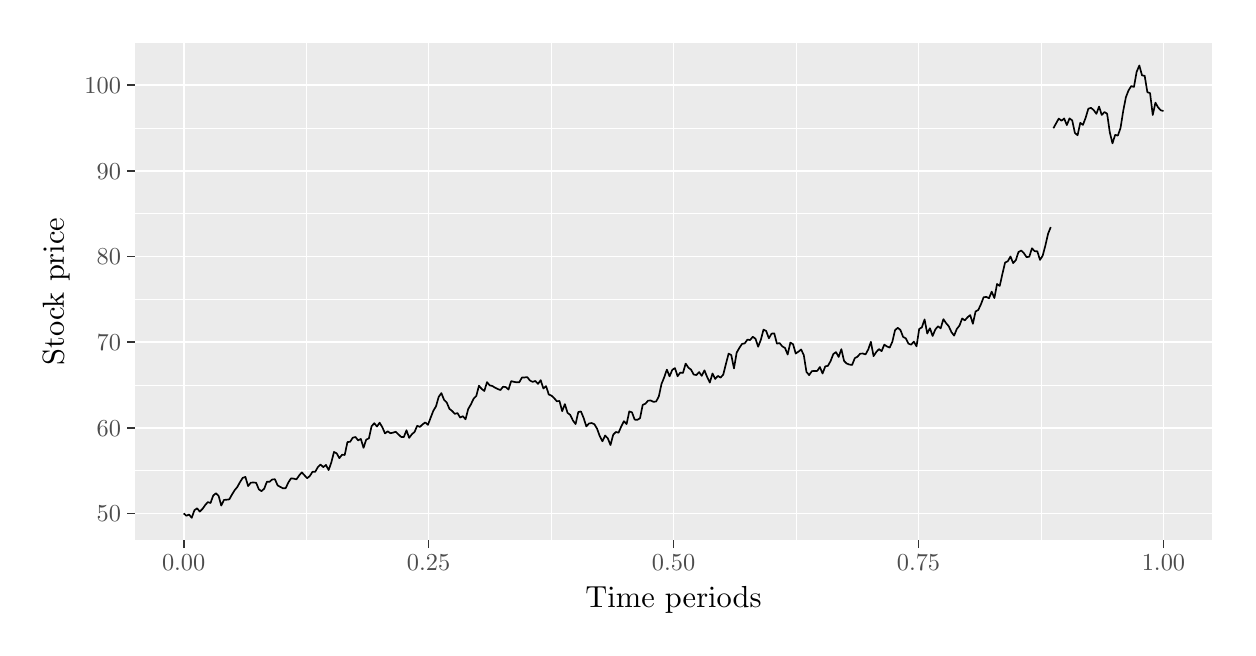
\begin{tikzpicture}[x=1pt,y=1pt]
\definecolor{fillColor}{RGB}{255,255,255}
\path[use as bounding box,fill=fillColor,fill opacity=0.00] (0,0) rectangle (433.62,216.81);
\begin{scope}
\path[clip] (  0.00,  0.00) rectangle (433.62,216.81);
\definecolor{drawColor}{RGB}{255,255,255}
\definecolor{fillColor}{RGB}{255,255,255}

\path[draw=drawColor,line width= 0.6pt,line join=round,line cap=round,fill=fillColor] (  0.00,  0.00) rectangle (433.62,216.81);
\end{scope}
\begin{scope}
\path[clip] ( 38.67, 31.53) rectangle (428.12,211.31);
\definecolor{fillColor}{gray}{0.92}

\path[fill=fillColor] ( 38.67, 31.53) rectangle (428.12,211.31);
\definecolor{drawColor}{RGB}{255,255,255}

\path[draw=drawColor,line width= 0.3pt,line join=round] ( 38.67, 56.77) --
	(428.12, 56.77);

\path[draw=drawColor,line width= 0.3pt,line join=round] ( 38.67, 87.71) --
	(428.12, 87.71);

\path[draw=drawColor,line width= 0.3pt,line join=round] ( 38.67,118.64) --
	(428.12,118.64);

\path[draw=drawColor,line width= 0.3pt,line join=round] ( 38.67,149.58) --
	(428.12,149.58);

\path[draw=drawColor,line width= 0.3pt,line join=round] ( 38.67,180.52) --
	(428.12,180.52);

\path[draw=drawColor,line width= 0.3pt,line join=round] (100.63, 31.53) --
	(100.63,211.31);

\path[draw=drawColor,line width= 0.3pt,line join=round] (189.14, 31.53) --
	(189.14,211.31);

\path[draw=drawColor,line width= 0.3pt,line join=round] (277.65, 31.53) --
	(277.65,211.31);

\path[draw=drawColor,line width= 0.3pt,line join=round] (366.16, 31.53) --
	(366.16,211.31);

\path[draw=drawColor,line width= 0.6pt,line join=round] ( 38.67, 41.30) --
	(428.12, 41.30);

\path[draw=drawColor,line width= 0.6pt,line join=round] ( 38.67, 72.24) --
	(428.12, 72.24);

\path[draw=drawColor,line width= 0.6pt,line join=round] ( 38.67,103.17) --
	(428.12,103.17);

\path[draw=drawColor,line width= 0.6pt,line join=round] ( 38.67,134.11) --
	(428.12,134.11);

\path[draw=drawColor,line width= 0.6pt,line join=round] ( 38.67,165.05) --
	(428.12,165.05);

\path[draw=drawColor,line width= 0.6pt,line join=round] ( 38.67,195.99) --
	(428.12,195.99);

\path[draw=drawColor,line width= 0.6pt,line join=round] ( 56.37, 31.53) --
	( 56.37,211.31);

\path[draw=drawColor,line width= 0.6pt,line join=round] (144.88, 31.53) --
	(144.88,211.31);

\path[draw=drawColor,line width= 0.6pt,line join=round] (233.39, 31.53) --
	(233.39,211.31);

\path[draw=drawColor,line width= 0.6pt,line join=round] (321.91, 31.53) --
	(321.91,211.31);

\path[draw=drawColor,line width= 0.6pt,line join=round] (410.42, 31.53) --
	(410.42,211.31);
\definecolor{drawColor}{RGB}{0,0,0}

\path[draw=drawColor,line width= 0.6pt,line join=round] ( 56.37, 41.30) --
	( 57.34, 40.44) --
	( 58.31, 40.89) --
	( 59.28, 39.70) --
	( 60.25, 42.44) --
	( 61.22, 43.13) --
	( 62.19, 41.95) --
	( 63.16, 42.90) --
	( 64.13, 44.27) --
	( 65.10, 45.39) --
	( 66.07, 45.04) --
	( 67.04, 47.73) --
	( 68.01, 48.55) --
	( 68.98, 47.66) --
	( 69.95, 44.13) --
	( 70.92, 46.15) --
	( 71.89, 46.24) --
	( 72.86, 46.37) --
	( 73.83, 48.12) --
	( 74.80, 49.68) --
	( 75.77, 50.86) --
	( 76.74, 52.62) --
	( 77.71, 54.15) --
	( 78.68, 54.45) --
	( 79.65, 51.16) --
	( 80.62, 52.39) --
	( 81.59, 52.46) --
	( 82.56, 52.36) --
	( 83.53, 49.99) --
	( 84.50, 49.34) --
	( 85.47, 50.22) --
	( 86.44, 52.73) --
	( 87.41, 52.72) --
	( 88.38, 53.56) --
	( 89.35, 53.63) --
	( 90.32, 51.41) --
	( 91.29, 50.86) --
	( 92.26, 50.35) --
	( 93.23, 50.41) --
	( 94.20, 52.47) --
	( 95.17, 53.97) --
	( 96.14, 53.85) --
	( 97.11, 53.58) --
	( 98.08, 54.97) --
	( 99.05, 56.12) --
	(100.02, 55.07) --
	(100.99, 54.00) --
	(101.96, 54.81) --
	(102.93, 56.34) --
	(103.90, 56.31) --
	(104.87, 58.05) --
	(105.84, 58.94) --
	(106.81, 58.01) --
	(107.78, 58.80) --
	(108.75, 56.95) --
	(109.72, 59.70) --
	(110.69, 63.50) --
	(111.66, 63.00) --
	(112.63, 61.26) --
	(113.60, 62.48) --
	(114.57, 62.41) --
	(115.54, 67.06) --
	(116.51, 67.17) --
	(117.48, 68.66) --
	(118.45, 68.90) --
	(119.42, 67.67) --
	(120.39, 68.21) --
	(121.36, 64.99) --
	(122.33, 67.93) --
	(123.30, 68.40) --
	(124.27, 72.77) --
	(125.24, 73.89) --
	(126.21, 72.69) --
	(127.18, 74.07) --
	(128.15, 72.43) --
	(129.12, 70.19) --
	(130.09, 70.94) --
	(131.06, 70.27) --
	(132.03, 70.46) --
	(133.00, 70.79) --
	(133.97, 69.84) --
	(134.94, 68.93) --
	(135.91, 68.86) --
	(136.88, 71.31) --
	(137.85, 68.57) --
	(138.82, 69.89) --
	(139.79, 70.71) --
	(140.76, 72.96) --
	(141.73, 72.55) --
	(142.70, 73.46) --
	(143.67, 74.17) --
	(144.64, 73.30) --
	(145.61, 75.86) --
	(146.58, 78.37) --
	(147.55, 79.97) --
	(148.52, 83.41) --
	(149.49, 84.76) --
	(150.46, 82.33) --
	(151.43, 81.36) --
	(152.40, 79.07) --
	(153.37, 78.31) --
	(154.34, 77.26) --
	(155.31, 77.54) --
	(156.28, 75.91) --
	(157.25, 76.42) --
	(158.22, 75.31) --
	(159.19, 79.03) --
	(160.16, 80.67) --
	(161.13, 82.73) --
	(162.10, 83.72) --
	(163.07, 87.42) --
	(164.04, 86.29) --
	(165.01, 85.53) --
	(165.98, 88.73) --
	(166.95, 87.56) --
	(167.92, 87.33) --
	(168.89, 86.71) --
	(169.86, 86.24) --
	(170.83, 85.86) --
	(171.80, 87.09) --
	(172.77, 86.92) --
	(173.74, 86.06) --
	(174.71, 89.09) --
	(175.68, 88.84) --
	(176.65, 88.66) --
	(177.62, 88.65) --
	(178.59, 90.37) --
	(179.56, 90.42) --
	(180.53, 90.54) --
	(181.50, 89.30) --
	(182.47, 88.81) --
	(183.44, 89.14) --
	(184.41, 88.10) --
	(185.38, 89.43) --
	(186.35, 86.43) --
	(187.32, 87.28) --
	(188.29, 84.27) --
	(189.26, 83.85) --
	(190.23, 82.96) --
	(191.20, 81.82) --
	(192.17, 81.90) --
	(193.14, 78.22) --
	(194.11, 80.79) --
	(195.08, 77.62) --
	(196.05, 76.89) --
	(197.02, 74.87) --
	(197.99, 73.58) --
	(198.96, 77.91) --
	(199.93, 78.13) --
	(200.90, 75.76) --
	(201.87, 72.73) --
	(202.84, 73.79) --
	(203.81, 73.95) --
	(204.78, 73.51) --
	(205.75, 71.89) --
	(206.72, 69.21) --
	(207.69, 67.35) --
	(208.66, 69.43) --
	(209.63, 68.43) --
	(210.60, 65.99) --
	(211.57, 69.72) --
	(212.54, 70.72) --
	(213.51, 70.45) --
	(214.48, 72.69) --
	(215.45, 74.61) --
	(216.42, 73.58) --
	(217.39, 78.14) --
	(218.36, 77.82) --
	(219.33, 75.18) --
	(220.30, 75.09) --
	(221.27, 75.69) --
	(222.24, 80.51) --
	(223.21, 80.92) --
	(224.18, 82.04) --
	(225.15, 82.08) --
	(226.12, 81.60) --
	(227.09, 81.72) --
	(228.06, 83.54) --
	(229.03, 88.06) --
	(230.00, 90.45) --
	(230.97, 93.25) --
	(231.94, 90.81) --
	(232.91, 93.13) --
	(233.88, 93.81) --
	(234.85, 90.86) --
	(235.82, 92.18) --
	(236.79, 92.05) --
	(237.76, 95.43) --
	(238.73, 93.97) --
	(239.70, 93.25) --
	(240.67, 91.46) --
	(241.64, 91.29) --
	(242.61, 92.36) --
	(243.58, 90.99) --
	(244.55, 92.98) --
	(245.52, 90.59) --
	(246.49, 88.57) --
	(247.46, 91.85) --
	(248.43, 89.88) --
	(249.40, 90.97) --
	(250.37, 90.36) --
	(251.34, 91.44) --
	(252.31, 95.30) --
	(253.28, 99.01) --
	(254.25, 98.49) --
	(255.22, 93.69) --
	(256.19, 99.39) --
	(257.16,101.09) --
	(258.13,102.53) --
	(259.10,102.72) --
	(260.07,104.09) --
	(261.04,103.94) --
	(262.01,105.11) --
	(262.98,104.42) --
	(263.95,101.53) --
	(264.92,103.99) --
	(265.89,107.69) --
	(266.86,107.20) --
	(267.83,104.55) --
	(268.80,106.24) --
	(269.77,106.36) --
	(270.74,102.62) --
	(271.71,102.84) --
	(272.68,101.64) --
	(273.65,101.09) --
	(274.62, 98.72) --
	(275.59,102.98) --
	(276.56,102.45) --
	(277.53, 99.06) --
	(278.50, 99.72) --
	(279.47,100.52) --
	(280.44, 98.53) --
	(281.41, 92.43) --
	(282.38, 91.26) --
	(283.35, 92.69) --
	(284.32, 92.77) --
	(285.29, 92.77) --
	(286.26, 94.19) --
	(287.23, 91.83) --
	(288.20, 94.41) --
	(289.17, 94.61) --
	(290.14, 96.36) --
	(291.11, 98.86) --
	(292.08, 99.57) --
	(293.05, 97.83) --
	(294.02,100.64) --
	(294.99, 96.41) --
	(295.96, 95.43) --
	(296.93, 95.08) --
	(297.90, 94.93) --
	(298.87, 97.38) --
	(299.84, 97.89) --
	(300.81, 99.01) --
	(301.78, 99.06) --
	(302.75, 98.73) --
	(303.72,100.49) --
	(304.69,103.29) --
	(305.66, 98.12) --
	(306.63, 99.61) --
	(307.60,100.66) --
	(308.57, 99.92) --
	(309.54,102.27) --
	(310.51,101.61) --
	(311.48,101.19) --
	(312.45,103.34) --
	(313.42,107.50) --
	(314.39,108.35) --
	(315.36,107.59) --
	(316.33,105.08) --
	(317.30,104.54) --
	(318.27,102.63) --
	(319.24,102.26) --
	(320.21,103.37) --
	(321.18,101.66) --
	(322.15,107.93) --
	(323.12,108.51) --
	(324.09,111.38) --
	(325.06,106.28) --
	(326.03,108.21) --
	(327.00,105.40) --
	(327.97,107.74) --
	(328.94,108.89) --
	(329.91,108.16) --
	(330.88,111.48) --
	(331.85,110.06) --
	(332.82,108.93) --
	(333.79,106.83) --
	(334.76,105.52) --
	(335.73,107.92) --
	(336.70,109.15) --
	(337.67,111.73) --
	(338.64,111.04) --
	(339.61,112.15) --
	(340.58,112.95) --
	(341.55,109.82) --
	(342.52,114.25) --
	(343.49,114.80) --
	(344.46,116.86) --
	(345.43,119.41) --
	(346.40,119.52) --
	(347.37,119.01) --
	(348.34,121.43) --
	(349.31,119.10) --
	(350.28,124.19) --
	(351.25,123.48) --
	(352.22,127.86) --
	(353.19,131.95) --
	(354.16,132.41) --
	(355.13,134.13) --
	(356.10,131.73) --
	(357.07,132.81) --
	(358.04,135.76) --
	(359.01,136.27) --
	(359.98,135.34) --
	(360.95,133.89) --
	(361.92,134.04) --
	(362.89,137.08) --
	(363.86,136.06) --
	(364.83,136.00) --
	(365.80,132.89) --
	(366.77,134.42) --
	(367.74,138.09) --
	(368.71,142.31) --
	(369.68,144.76);

\path[draw=drawColor,line width= 0.6pt,line join=round] (370.65,180.47) --
	(371.62,182.25) --
	(372.59,183.97) --
	(373.56,183.17) --
	(374.53,184.00) --
	(375.50,181.61) --
	(376.47,184.02) --
	(377.44,183.30) --
	(378.41,178.76) --
	(379.38,177.93) --
	(380.35,182.42) --
	(381.32,181.68) --
	(382.29,184.25) --
	(383.26,187.52) --
	(384.23,187.84) --
	(385.20,187.03) --
	(386.17,185.67) --
	(387.14,188.30) --
	(388.11,185.26) --
	(389.08,186.33) --
	(390.05,185.72) --
	(391.02,179.01) --
	(391.99,175.01) --
	(392.96,178.09) --
	(393.93,177.80) --
	(394.90,180.55) --
	(395.87,186.72) --
	(396.84,191.69) --
	(397.81,194.17) --
	(398.78,195.71) --
	(399.75,195.39) --
	(400.72,200.85) --
	(401.69,203.14) --
	(402.66,199.59) --
	(403.63,199.39) --
	(404.60,193.48) --
	(405.57,193.16) --
	(406.54,185.25) --
	(407.51,189.70) --
	(408.48,187.99) --
	(409.45,186.94) --
	(410.42,186.71);
\end{scope}
\begin{scope}
\path[clip] (  0.00,  0.00) rectangle (433.62,216.81);
\definecolor{drawColor}{gray}{0.30}

\node[text=drawColor,anchor=base east,inner sep=0pt, outer sep=0pt, scale=  0.88] at ( 33.72, 38.27) {50};

\node[text=drawColor,anchor=base east,inner sep=0pt, outer sep=0pt, scale=  0.88] at ( 33.72, 69.21) {60};

\node[text=drawColor,anchor=base east,inner sep=0pt, outer sep=0pt, scale=  0.88] at ( 33.72,100.14) {70};

\node[text=drawColor,anchor=base east,inner sep=0pt, outer sep=0pt, scale=  0.88] at ( 33.72,131.08) {80};

\node[text=drawColor,anchor=base east,inner sep=0pt, outer sep=0pt, scale=  0.88] at ( 33.72,162.02) {90};

\node[text=drawColor,anchor=base east,inner sep=0pt, outer sep=0pt, scale=  0.88] at ( 33.72,192.96) {100};
\end{scope}
\begin{scope}
\path[clip] (  0.00,  0.00) rectangle (433.62,216.81);
\definecolor{drawColor}{gray}{0.20}

\path[draw=drawColor,line width= 0.6pt,line join=round] ( 35.92, 41.30) --
	( 38.67, 41.30);

\path[draw=drawColor,line width= 0.6pt,line join=round] ( 35.92, 72.24) --
	( 38.67, 72.24);

\path[draw=drawColor,line width= 0.6pt,line join=round] ( 35.92,103.17) --
	( 38.67,103.17);

\path[draw=drawColor,line width= 0.6pt,line join=round] ( 35.92,134.11) --
	( 38.67,134.11);

\path[draw=drawColor,line width= 0.6pt,line join=round] ( 35.92,165.05) --
	( 38.67,165.05);

\path[draw=drawColor,line width= 0.6pt,line join=round] ( 35.92,195.99) --
	( 38.67,195.99);
\end{scope}
\begin{scope}
\path[clip] (  0.00,  0.00) rectangle (433.62,216.81);
\definecolor{drawColor}{gray}{0.20}

\path[draw=drawColor,line width= 0.6pt,line join=round] ( 56.37, 28.78) --
	( 56.37, 31.53);

\path[draw=drawColor,line width= 0.6pt,line join=round] (144.88, 28.78) --
	(144.88, 31.53);

\path[draw=drawColor,line width= 0.6pt,line join=round] (233.39, 28.78) --
	(233.39, 31.53);

\path[draw=drawColor,line width= 0.6pt,line join=round] (321.91, 28.78) --
	(321.91, 31.53);

\path[draw=drawColor,line width= 0.6pt,line join=round] (410.42, 28.78) --
	(410.42, 31.53);
\end{scope}
\begin{scope}
\path[clip] (  0.00,  0.00) rectangle (433.62,216.81);
\definecolor{drawColor}{gray}{0.30}

\node[text=drawColor,anchor=base,inner sep=0pt, outer sep=0pt, scale=  0.88] at ( 56.37, 20.52) {0.00};

\node[text=drawColor,anchor=base,inner sep=0pt, outer sep=0pt, scale=  0.88] at (144.88, 20.52) {0.25};

\node[text=drawColor,anchor=base,inner sep=0pt, outer sep=0pt, scale=  0.88] at (233.39, 20.52) {0.50};

\node[text=drawColor,anchor=base,inner sep=0pt, outer sep=0pt, scale=  0.88] at (321.91, 20.52) {0.75};

\node[text=drawColor,anchor=base,inner sep=0pt, outer sep=0pt, scale=  0.88] at (410.42, 20.52) {1.00};
\end{scope}
\begin{scope}
\path[clip] (  0.00,  0.00) rectangle (433.62,216.81);
\definecolor{drawColor}{RGB}{0,0,0}

\node[text=drawColor,anchor=base,inner sep=0pt, outer sep=0pt, scale=  1.10] at (233.39,  7.44) {Time periods};
\end{scope}
\begin{scope}
\path[clip] (  0.00,  0.00) rectangle (433.62,216.81);
\definecolor{drawColor}{RGB}{0,0,0}

\node[text=drawColor,rotate= 90.00,anchor=base,inner sep=0pt, outer sep=0pt, scale=  1.10] at ( 13.08,121.42) {Stock price};
\end{scope}
\end{tikzpicture}
 
  \floatfoot{Simulation of one Merton mixed jump-diffusion time serie. Data have been output by the R function \textit{sstoch\_jump()} which is an implementation of equation \cref{eq:other:merton:pde} (see appendix \ref{sub:r:time:merton}, for more information). The parameters passed to the function are:  $S(0) = 50$,   $T = 1$ (in year, along with a time step of 365 measures per year),  $\sigma = 0.2$, $\alpha = 0.5$,  $\lambda = 2$,  $\mu = 0.05$, and $\delta = 0.1$.}
  \caption{Merton mixed jump-diffusion time serie}
  \label{p:other:merton:path}
\end{figure}




%%%%%%%%%%%%%%%%%%%%%%%%%%%%%%%%%%%%%%%%%%%%%%%%
% SUBSECTION: Skewness
%%%%%%%%%%%%%%%%%%%%%%%%%%%%%%%%%%%%%%%%%%%%%%%%
\subsection{Impact on the skewness log--return}
\label{sub:MertonSkewness}

The way to influence the direction of the distibution's shape is achieved by moving the cursor of the expected value of jump impact, in other word, by changing the value of the parameter $\mu$. The figure [REF] shows how the density's shape of the log--return may vary along with this parameter.


\begin{figure}[H]
\centering
% Created by tikzDevice version 0.11 on 2018-04-10 23:12:32
% !TEX encoding = UTF-8 Unicode
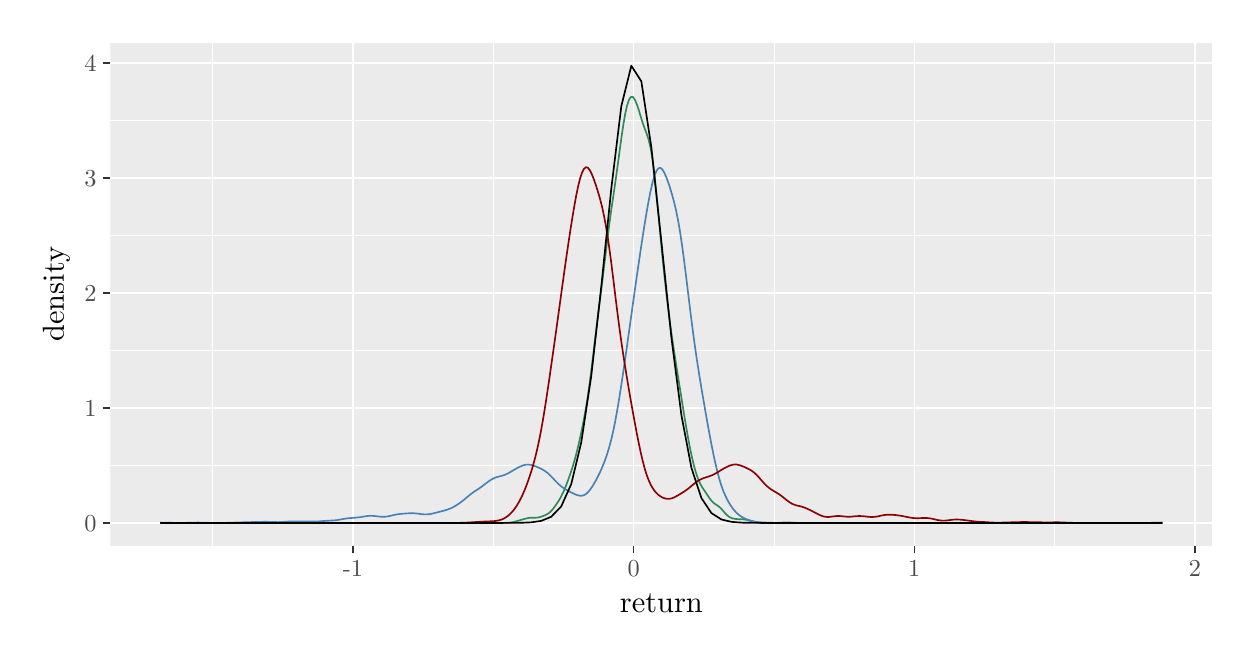
\begin{tikzpicture}[x=1pt,y=1pt]
\definecolor{fillColor}{RGB}{255,255,255}
\path[use as bounding box,fill=fillColor,fill opacity=0.00] (0,0) rectangle (433.62,216.81);
\begin{scope}
\path[clip] (  0.00,  0.00) rectangle (433.62,216.81);
\definecolor{drawColor}{RGB}{255,255,255}
\definecolor{fillColor}{RGB}{255,255,255}

\path[draw=drawColor,line width= 0.6pt,line join=round,line cap=round,fill=fillColor] (  0.00,  0.00) rectangle (433.62,216.81);
\end{scope}
\begin{scope}
\path[clip] ( 29.87, 29.59) rectangle (428.12,211.31);
\definecolor{fillColor}{gray}{0.92}

\path[fill=fillColor] ( 29.87, 29.59) rectangle (428.12,211.31);
\definecolor{drawColor}{RGB}{255,255,255}

\path[draw=drawColor,line width= 0.3pt,line join=round] ( 29.87, 58.62) --
	(428.12, 58.62);

\path[draw=drawColor,line width= 0.3pt,line join=round] ( 29.87,100.17) --
	(428.12,100.17);

\path[draw=drawColor,line width= 0.3pt,line join=round] ( 29.87,141.71) --
	(428.12,141.71);

\path[draw=drawColor,line width= 0.3pt,line join=round] ( 29.87,183.26) --
	(428.12,183.26);

\path[draw=drawColor,line width= 0.3pt,line join=round] ( 66.80, 29.59) --
	( 66.80,211.31);

\path[draw=drawColor,line width= 0.3pt,line join=round] (168.24, 29.59) --
	(168.24,211.31);

\path[draw=drawColor,line width= 0.3pt,line join=round] (269.68, 29.59) --
	(269.68,211.31);

\path[draw=drawColor,line width= 0.3pt,line join=round] (371.11, 29.59) --
	(371.11,211.31);

\path[draw=drawColor,line width= 0.6pt,line join=round] ( 29.87, 37.85) --
	(428.12, 37.85);

\path[draw=drawColor,line width= 0.6pt,line join=round] ( 29.87, 79.39) --
	(428.12, 79.39);

\path[draw=drawColor,line width= 0.6pt,line join=round] ( 29.87,120.94) --
	(428.12,120.94);

\path[draw=drawColor,line width= 0.6pt,line join=round] ( 29.87,162.49) --
	(428.12,162.49);

\path[draw=drawColor,line width= 0.6pt,line join=round] ( 29.87,204.03) --
	(428.12,204.03);

\path[draw=drawColor,line width= 0.6pt,line join=round] (117.52, 29.59) --
	(117.52,211.31);

\path[draw=drawColor,line width= 0.6pt,line join=round] (218.96, 29.59) --
	(218.96,211.31);

\path[draw=drawColor,line width= 0.6pt,line join=round] (320.39, 29.59) --
	(320.39,211.31);

\path[draw=drawColor,line width= 0.6pt,line join=round] (421.83, 29.59) --
	(421.83,211.31);
\definecolor{drawColor}{RGB}{46,139,87}

\path[draw=drawColor,line width= 0.6pt,line join=round] ( 47.97, 37.85) --
	( 48.68, 37.85) --
	( 49.39, 37.85) --
	( 50.10, 37.85) --
	( 50.81, 37.85) --
	( 51.51, 37.85) --
	( 52.22, 37.85) --
	( 52.93, 37.85) --
	( 53.64, 37.85) --
	( 54.35, 37.85) --
	( 55.06, 37.85) --
	( 55.76, 37.85) --
	( 56.47, 37.85) --
	( 57.18, 37.85) --
	( 57.89, 37.85) --
	( 58.60, 37.85) --
	( 59.31, 37.85) --
	( 60.02, 37.85) --
	( 60.72, 37.85) --
	( 61.43, 37.85) --
	( 62.14, 37.85) --
	( 62.85, 37.85) --
	( 63.56, 37.85) --
	( 64.27, 37.85) --
	( 64.98, 37.85) --
	( 65.68, 37.85) --
	( 66.39, 37.85) --
	( 67.10, 37.85) --
	( 67.81, 37.85) --
	( 68.52, 37.85) --
	( 69.23, 37.85) --
	( 69.93, 37.85) --
	( 70.64, 37.85) --
	( 71.35, 37.85) --
	( 72.06, 37.85) --
	( 72.77, 37.85) --
	( 73.48, 37.85) --
	( 74.19, 37.85) --
	( 74.89, 37.85) --
	( 75.60, 37.85) --
	( 76.31, 37.85) --
	( 77.02, 37.85) --
	( 77.73, 37.85) --
	( 78.44, 37.85) --
	( 79.15, 37.85) --
	( 79.85, 37.85) --
	( 80.56, 37.85) --
	( 81.27, 37.85) --
	( 81.98, 37.85) --
	( 82.69, 37.85) --
	( 83.40, 37.85) --
	( 84.10, 37.85) --
	( 84.81, 37.85) --
	( 85.52, 37.85) --
	( 86.23, 37.85) --
	( 86.94, 37.85) --
	( 87.65, 37.85) --
	( 88.36, 37.85) --
	( 89.06, 37.85) --
	( 89.77, 37.85) --
	( 90.48, 37.85) --
	( 91.19, 37.85) --
	( 91.90, 37.85) --
	( 92.61, 37.85) --
	( 93.32, 37.85) --
	( 94.02, 37.85) --
	( 94.73, 37.85) --
	( 95.44, 37.85) --
	( 96.15, 37.85) --
	( 96.86, 37.85) --
	( 97.57, 37.85) --
	( 98.28, 37.85) --
	( 98.98, 37.85) --
	( 99.69, 37.85) --
	(100.40, 37.85) --
	(101.11, 37.85) --
	(101.82, 37.85) --
	(102.53, 37.85) --
	(103.23, 37.85) --
	(103.94, 37.85) --
	(104.65, 37.85) --
	(105.36, 37.85) --
	(106.07, 37.85) --
	(106.78, 37.85) --
	(107.49, 37.85) --
	(108.19, 37.85) --
	(108.90, 37.85) --
	(109.61, 37.85) --
	(110.32, 37.85) --
	(111.03, 37.85) --
	(111.74, 37.85) --
	(112.45, 37.85) --
	(113.15, 37.85) --
	(113.86, 37.85) --
	(114.57, 37.85) --
	(115.28, 37.85) --
	(115.99, 37.85) --
	(116.70, 37.85) --
	(117.40, 37.85) --
	(118.11, 37.85) --
	(118.82, 37.85) --
	(119.53, 37.85) --
	(120.24, 37.85) --
	(120.95, 37.85) --
	(121.66, 37.85) --
	(122.36, 37.85) --
	(123.07, 37.85) --
	(123.78, 37.85) --
	(124.49, 37.85) --
	(125.20, 37.85) --
	(125.91, 37.85) --
	(126.62, 37.85) --
	(127.32, 37.85) --
	(128.03, 37.85) --
	(128.74, 37.85) --
	(129.45, 37.85) --
	(130.16, 37.85) --
	(130.87, 37.85) --
	(131.57, 37.85) --
	(132.28, 37.85) --
	(132.99, 37.85) --
	(133.70, 37.85) --
	(134.41, 37.85) --
	(135.12, 37.85) --
	(135.83, 37.85) --
	(136.53, 37.85) --
	(137.24, 37.85) --
	(137.95, 37.85) --
	(138.66, 37.85) --
	(139.37, 37.85) --
	(140.08, 37.85) --
	(140.79, 37.85) --
	(141.49, 37.85) --
	(142.20, 37.85) --
	(142.91, 37.85) --
	(143.62, 37.85) --
	(144.33, 37.85) --
	(145.04, 37.85) --
	(145.74, 37.85) --
	(146.45, 37.85) --
	(147.16, 37.85) --
	(147.87, 37.85) --
	(148.58, 37.85) --
	(149.29, 37.85) --
	(150.00, 37.85) --
	(150.70, 37.85) --
	(151.41, 37.85) --
	(152.12, 37.85) --
	(152.83, 37.85) --
	(153.54, 37.85) --
	(154.25, 37.85) --
	(154.96, 37.85) --
	(155.66, 37.85) --
	(156.37, 37.85) --
	(157.08, 37.85) --
	(157.79, 37.85) --
	(158.50, 37.86) --
	(159.21, 37.87) --
	(159.92, 37.89) --
	(160.62, 37.93) --
	(161.33, 37.97) --
	(162.04, 38.01) --
	(162.75, 38.03) --
	(163.46, 38.02) --
	(164.17, 38.00) --
	(164.87, 37.96) --
	(165.58, 37.92) --
	(166.29, 37.88) --
	(167.00, 37.86) --
	(167.71, 37.85) --
	(168.42, 37.85) --
	(169.13, 37.85) --
	(169.83, 37.85) --
	(170.54, 37.85) --
	(171.25, 37.85) --
	(171.96, 37.85) --
	(172.67, 37.87) --
	(173.38, 37.89) --
	(174.09, 37.95) --
	(174.79, 38.04) --
	(175.50, 38.18) --
	(176.21, 38.35) --
	(176.92, 38.55) --
	(177.63, 38.76) --
	(178.34, 38.97) --
	(179.04, 39.16) --
	(179.75, 39.35) --
	(180.46, 39.53) --
	(181.17, 39.67) --
	(181.88, 39.74) --
	(182.59, 39.74) --
	(183.30, 39.73) --
	(184.00, 39.76) --
	(184.71, 39.87) --
	(185.42, 40.06) --
	(186.13, 40.31) --
	(186.84, 40.59) --
	(187.55, 40.92) --
	(188.26, 41.35) --
	(188.96, 41.95) --
	(189.67, 42.72) --
	(190.38, 43.64) --
	(191.09, 44.65) --
	(191.80, 45.73) --
	(192.51, 46.92) --
	(193.21, 48.27) --
	(193.92, 49.81) --
	(194.63, 51.56) --
	(195.34, 53.46) --
	(196.05, 55.49) --
	(196.76, 57.64) --
	(197.47, 59.97) --
	(198.17, 62.53) --
	(198.88, 65.35) --
	(199.59, 68.45) --
	(200.30, 71.81) --
	(201.01, 75.44) --
	(201.72, 79.40) --
	(202.43, 83.82) --
	(203.13, 88.81) --
	(203.84, 94.36) --
	(204.55,100.28) --
	(205.26,106.28) --
	(205.97,112.07) --
	(206.68,117.64) --
	(207.39,123.17) --
	(208.09,128.86) --
	(208.80,134.75) --
	(209.51,140.63) --
	(210.22,146.18) --
	(210.93,151.28) --
	(211.64,156.10) --
	(212.34,160.94) --
	(213.05,166.00) --
	(213.76,171.26) --
	(214.47,176.49) --
	(215.18,181.37) --
	(215.89,185.54) --
	(216.60,188.75) --
	(217.30,190.84) --
	(218.01,191.81) --
	(218.72,191.74) --
	(219.43,190.77) --
	(220.14,189.08) --
	(220.85,186.92) --
	(221.56,184.56) --
	(222.26,182.32) --
	(222.97,180.34) --
	(223.68,178.49) --
	(224.39,176.31) --
	(225.10,173.28) --
	(225.81,168.97) --
	(226.51,163.33) --
	(227.22,156.61) --
	(227.93,149.23) --
	(228.64,141.66) --
	(229.35,134.28) --
	(230.06,127.33) --
	(230.77,120.90) --
	(231.47,114.98) --
	(232.18,109.53) --
	(232.89,104.47) --
	(233.60, 99.71) --
	(234.31, 95.15) --
	(235.02, 90.69) --
	(235.73, 86.25) --
	(236.43, 81.81) --
	(237.14, 77.38) --
	(237.85, 73.08) --
	(238.56, 69.00) --
	(239.27, 65.24) --
	(239.98, 61.85) --
	(240.68, 58.86) --
	(241.39, 56.28) --
	(242.10, 54.14) --
	(242.81, 52.43) --
	(243.52, 51.09) --
	(244.23, 49.97) --
	(244.94, 48.94) --
	(245.64, 47.88) --
	(246.35, 46.83) --
	(247.06, 45.89) --
	(247.77, 45.16) --
	(248.48, 44.63) --
	(249.19, 44.18) --
	(249.90, 43.66) --
	(250.60, 42.98) --
	(251.31, 42.18) --
	(252.02, 41.36) --
	(252.73, 40.64) --
	(253.44, 40.08) --
	(254.15, 39.69) --
	(254.85, 39.46) --
	(255.56, 39.32) --
	(256.27, 39.24) --
	(256.98, 39.20) --
	(257.69, 39.18) --
	(258.40, 39.16) --
	(259.11, 39.09) --
	(259.81, 38.96) --
	(260.52, 38.76) --
	(261.23, 38.54) --
	(261.94, 38.31) --
	(262.65, 38.13) --
	(263.36, 38.00) --
	(264.07, 37.92) --
	(264.77, 37.88) --
	(265.48, 37.86) --
	(266.19, 37.85) --
	(266.90, 37.85) --
	(267.61, 37.85) --
	(268.32, 37.85) --
	(269.03, 37.85) --
	(269.73, 37.85) --
	(270.44, 37.87) --
	(271.15, 37.89) --
	(271.86, 37.92) --
	(272.57, 37.96) --
	(273.28, 38.00) --
	(273.98, 38.03) --
	(274.69, 38.03) --
	(275.40, 38.00) --
	(276.11, 37.96) --
	(276.82, 37.92) --
	(277.53, 37.89) --
	(278.24, 37.87) --
	(278.94, 37.85) --
	(279.65, 37.85) --
	(280.36, 37.85) --
	(281.07, 37.85) --
	(281.78, 37.85) --
	(282.49, 37.85) --
	(283.20, 37.85) --
	(283.90, 37.85) --
	(284.61, 37.85) --
	(285.32, 37.85) --
	(286.03, 37.85) --
	(286.74, 37.85) --
	(287.45, 37.85) --
	(288.15, 37.85) --
	(288.86, 37.85) --
	(289.57, 37.85) --
	(290.28, 37.85) --
	(290.99, 37.85) --
	(291.70, 37.85) --
	(292.41, 37.85) --
	(293.11, 37.85) --
	(293.82, 37.85) --
	(294.53, 37.85) --
	(295.24, 37.85) --
	(295.95, 37.85) --
	(296.66, 37.85) --
	(297.37, 37.85) --
	(298.07, 37.85) --
	(298.78, 37.85) --
	(299.49, 37.85) --
	(300.20, 37.85) --
	(300.91, 37.85) --
	(301.62, 37.85) --
	(302.32, 37.85) --
	(303.03, 37.85) --
	(303.74, 37.85) --
	(304.45, 37.85) --
	(305.16, 37.85) --
	(305.87, 37.85) --
	(306.58, 37.85) --
	(307.28, 37.85) --
	(307.99, 37.85) --
	(308.70, 37.85) --
	(309.41, 37.85) --
	(310.12, 37.85) --
	(310.83, 37.85) --
	(311.54, 37.85) --
	(312.24, 37.85) --
	(312.95, 37.85) --
	(313.66, 37.85) --
	(314.37, 37.85) --
	(315.08, 37.85) --
	(315.79, 37.85) --
	(316.49, 37.85) --
	(317.20, 37.85) --
	(317.91, 37.85) --
	(318.62, 37.85) --
	(319.33, 37.85) --
	(320.04, 37.85) --
	(320.75, 37.85) --
	(321.45, 37.85) --
	(322.16, 37.85) --
	(322.87, 37.85) --
	(323.58, 37.85) --
	(324.29, 37.85) --
	(325.00, 37.85) --
	(325.71, 37.85) --
	(326.41, 37.85) --
	(327.12, 37.85) --
	(327.83, 37.85) --
	(328.54, 37.85) --
	(329.25, 37.85) --
	(329.96, 37.85) --
	(330.67, 37.85) --
	(331.37, 37.85) --
	(332.08, 37.85) --
	(332.79, 37.85) --
	(333.50, 37.85) --
	(334.21, 37.85) --
	(334.92, 37.85) --
	(335.62, 37.85) --
	(336.33, 37.85) --
	(337.04, 37.85) --
	(337.75, 37.85) --
	(338.46, 37.85) --
	(339.17, 37.85) --
	(339.88, 37.85) --
	(340.58, 37.85) --
	(341.29, 37.85) --
	(342.00, 37.85) --
	(342.71, 37.85) --
	(343.42, 37.85) --
	(344.13, 37.85) --
	(344.84, 37.85) --
	(345.54, 37.85) --
	(346.25, 37.85) --
	(346.96, 37.85) --
	(347.67, 37.85) --
	(348.38, 37.85) --
	(349.09, 37.85) --
	(349.79, 37.85) --
	(350.50, 37.85) --
	(351.21, 37.85) --
	(351.92, 37.85) --
	(352.63, 37.85) --
	(353.34, 37.85) --
	(354.05, 37.85) --
	(354.75, 37.85) --
	(355.46, 37.85) --
	(356.17, 37.85) --
	(356.88, 37.85) --
	(357.59, 37.85) --
	(358.30, 37.85) --
	(359.01, 37.85) --
	(359.71, 37.85) --
	(360.42, 37.85) --
	(361.13, 37.85) --
	(361.84, 37.85) --
	(362.55, 37.85) --
	(363.26, 37.85) --
	(363.96, 37.85) --
	(364.67, 37.85) --
	(365.38, 37.85) --
	(366.09, 37.85) --
	(366.80, 37.85) --
	(367.51, 37.85) --
	(368.22, 37.85) --
	(368.92, 37.85) --
	(369.63, 37.85) --
	(370.34, 37.85) --
	(371.05, 37.85) --
	(371.76, 37.85) --
	(372.47, 37.85) --
	(373.18, 37.85) --
	(373.88, 37.85) --
	(374.59, 37.85) --
	(375.30, 37.85) --
	(376.01, 37.85) --
	(376.72, 37.85) --
	(377.43, 37.85) --
	(378.13, 37.85) --
	(378.84, 37.85) --
	(379.55, 37.85) --
	(380.26, 37.85) --
	(380.97, 37.85) --
	(381.68, 37.85) --
	(382.39, 37.85) --
	(383.09, 37.85) --
	(383.80, 37.85) --
	(384.51, 37.85) --
	(385.22, 37.85) --
	(385.93, 37.85) --
	(386.64, 37.85) --
	(387.35, 37.85) --
	(388.05, 37.85) --
	(388.76, 37.85) --
	(389.47, 37.85) --
	(390.18, 37.85) --
	(390.89, 37.85) --
	(391.60, 37.85) --
	(392.31, 37.85) --
	(393.01, 37.85) --
	(393.72, 37.85) --
	(394.43, 37.85) --
	(395.14, 37.85) --
	(395.85, 37.85) --
	(396.56, 37.85) --
	(397.26, 37.85) --
	(397.97, 37.85) --
	(398.68, 37.85) --
	(399.39, 37.85) --
	(400.10, 37.85) --
	(400.81, 37.85) --
	(401.52, 37.85) --
	(402.22, 37.85) --
	(402.93, 37.85) --
	(403.64, 37.85) --
	(404.35, 37.85) --
	(405.06, 37.85) --
	(405.77, 37.85) --
	(406.48, 37.85) --
	(407.18, 37.85) --
	(407.89, 37.85) --
	(408.60, 37.85) --
	(409.31, 37.85) --
	(410.02, 37.85);
\definecolor{drawColor}{RGB}{70,130,180}

\path[draw=drawColor,line width= 0.6pt,line join=round] ( 47.97, 37.98) --
	( 48.68, 37.97) --
	( 49.39, 37.96) --
	( 50.10, 37.94) --
	( 50.81, 37.92) --
	( 51.51, 37.90) --
	( 52.22, 37.88) --
	( 52.93, 37.87) --
	( 53.64, 37.86) --
	( 54.35, 37.86) --
	( 55.06, 37.86) --
	( 55.76, 37.86) --
	( 56.47, 37.87) --
	( 57.18, 37.88) --
	( 57.89, 37.90) --
	( 58.60, 37.91) --
	( 59.31, 37.94) --
	( 60.02, 37.96) --
	( 60.72, 37.97) --
	( 61.43, 37.98) --
	( 62.14, 37.97) --
	( 62.85, 37.96) --
	( 63.56, 37.94) --
	( 64.27, 37.92) --
	( 64.98, 37.90) --
	( 65.68, 37.88) --
	( 66.39, 37.87) --
	( 67.10, 37.86) --
	( 67.81, 37.86) --
	( 68.52, 37.85) --
	( 69.23, 37.85) --
	( 69.93, 37.86) --
	( 70.64, 37.86) --
	( 71.35, 37.87) --
	( 72.06, 37.89) --
	( 72.77, 37.91) --
	( 73.48, 37.93) --
	( 74.19, 37.96) --
	( 74.89, 37.98) --
	( 75.60, 38.01) --
	( 76.31, 38.03) --
	( 77.02, 38.05) --
	( 77.73, 38.07) --
	( 78.44, 38.09) --
	( 79.15, 38.12) --
	( 79.85, 38.14) --
	( 80.56, 38.15) --
	( 81.27, 38.17) --
	( 81.98, 38.18) --
	( 82.69, 38.19) --
	( 83.40, 38.20) --
	( 84.10, 38.22) --
	( 84.81, 38.24) --
	( 85.52, 38.26) --
	( 86.23, 38.26) --
	( 86.94, 38.25) --
	( 87.65, 38.23) --
	( 88.36, 38.20) --
	( 89.06, 38.18) --
	( 89.77, 38.16) --
	( 90.48, 38.15) --
	( 91.19, 38.17) --
	( 91.90, 38.20) --
	( 92.61, 38.24) --
	( 93.32, 38.29) --
	( 94.02, 38.33) --
	( 94.73, 38.36) --
	( 95.44, 38.38) --
	( 96.15, 38.39) --
	( 96.86, 38.39) --
	( 97.57, 38.39) --
	( 98.28, 38.40) --
	( 98.98, 38.40) --
	( 99.69, 38.41) --
	(100.40, 38.40) --
	(101.11, 38.39) --
	(101.82, 38.38) --
	(102.53, 38.37) --
	(103.23, 38.36) --
	(103.94, 38.36) --
	(104.65, 38.38) --
	(105.36, 38.42) --
	(106.07, 38.47) --
	(106.78, 38.53) --
	(107.49, 38.58) --
	(108.19, 38.63) --
	(108.90, 38.67) --
	(109.61, 38.70) --
	(110.32, 38.74) --
	(111.03, 38.80) --
	(111.74, 38.88) --
	(112.45, 38.99) --
	(113.15, 39.11) --
	(113.86, 39.24) --
	(114.57, 39.37) --
	(115.28, 39.47) --
	(115.99, 39.56) --
	(116.70, 39.62) --
	(117.40, 39.67) --
	(118.11, 39.72) --
	(118.82, 39.78) --
	(119.53, 39.86) --
	(120.24, 39.95) --
	(120.95, 40.07) --
	(121.66, 40.19) --
	(122.36, 40.30) --
	(123.07, 40.38) --
	(123.78, 40.42) --
	(124.49, 40.41) --
	(125.20, 40.36) --
	(125.91, 40.28) --
	(126.62, 40.19) --
	(127.32, 40.12) --
	(128.03, 40.07) --
	(128.74, 40.07) --
	(129.45, 40.12) --
	(130.16, 40.23) --
	(130.87, 40.37) --
	(131.57, 40.54) --
	(132.28, 40.70) --
	(132.99, 40.86) --
	(133.70, 40.98) --
	(134.41, 41.07) --
	(135.12, 41.14) --
	(135.83, 41.20) --
	(136.53, 41.25) --
	(137.24, 41.30) --
	(137.95, 41.34) --
	(138.66, 41.36) --
	(139.37, 41.34) --
	(140.08, 41.30) --
	(140.79, 41.23) --
	(141.49, 41.14) --
	(142.20, 41.04) --
	(142.91, 40.97) --
	(143.62, 40.93) --
	(144.33, 40.95) --
	(145.04, 41.01) --
	(145.74, 41.12) --
	(146.45, 41.27) --
	(147.16, 41.45) --
	(147.87, 41.63) --
	(148.58, 41.82) --
	(149.29, 42.00) --
	(150.00, 42.18) --
	(150.70, 42.37) --
	(151.41, 42.58) --
	(152.12, 42.83) --
	(152.83, 43.11) --
	(153.54, 43.45) --
	(154.25, 43.83) --
	(154.96, 44.25) --
	(155.66, 44.72) --
	(156.37, 45.22) --
	(157.08, 45.76) --
	(157.79, 46.33) --
	(158.50, 46.92) --
	(159.21, 47.51) --
	(159.92, 48.09) --
	(160.62, 48.63) --
	(161.33, 49.13) --
	(162.04, 49.60) --
	(162.75, 50.06) --
	(163.46, 50.54) --
	(164.17, 51.05) --
	(164.87, 51.59) --
	(165.58, 52.14) --
	(166.29, 52.67) --
	(167.00, 53.17) --
	(167.71, 53.60) --
	(168.42, 53.96) --
	(169.13, 54.25) --
	(169.83, 54.48) --
	(170.54, 54.68) --
	(171.25, 54.87) --
	(171.96, 55.08) --
	(172.67, 55.35) --
	(173.38, 55.67) --
	(174.09, 56.05) --
	(174.79, 56.46) --
	(175.50, 56.88) --
	(176.21, 57.29) --
	(176.92, 57.69) --
	(177.63, 58.06) --
	(178.34, 58.38) --
	(179.04, 58.65) --
	(179.75, 58.84) --
	(180.46, 58.93) --
	(181.17, 58.92) --
	(181.88, 58.81) --
	(182.59, 58.63) --
	(183.30, 58.38) --
	(184.00, 58.11) --
	(184.71, 57.80) --
	(185.42, 57.47) --
	(186.13, 57.09) --
	(186.84, 56.66) --
	(187.55, 56.15) --
	(188.26, 55.56) --
	(188.96, 54.88) --
	(189.67, 54.14) --
	(190.38, 53.37) --
	(191.09, 52.62) --
	(191.80, 51.92) --
	(192.51, 51.29) --
	(193.21, 50.74) --
	(193.92, 50.26) --
	(194.63, 49.83) --
	(195.34, 49.43) --
	(196.05, 49.06) --
	(196.76, 48.69) --
	(197.47, 48.35) --
	(198.17, 48.05) --
	(198.88, 47.82) --
	(199.59, 47.68) --
	(200.30, 47.69) --
	(201.01, 47.88) --
	(201.72, 48.29) --
	(202.43, 48.91) --
	(203.13, 49.74) --
	(203.84, 50.74) --
	(204.55, 51.87) --
	(205.26, 53.11) --
	(205.97, 54.45) --
	(206.68, 55.88) --
	(207.39, 57.44) --
	(208.09, 59.14) --
	(208.80, 61.02) --
	(209.51, 63.12) --
	(210.22, 65.49) --
	(210.93, 68.20) --
	(211.64, 71.28) --
	(212.34, 74.77) --
	(213.05, 78.66) --
	(213.76, 82.91) --
	(214.47, 87.43) --
	(215.18, 92.16) --
	(215.89, 97.03) --
	(216.60,101.99) --
	(217.30,107.01) --
	(218.01,112.07) --
	(218.72,117.14) --
	(219.43,122.19) --
	(220.14,127.18) --
	(220.85,132.08) --
	(221.56,136.87) --
	(222.26,141.52) --
	(222.97,146.01) --
	(223.68,150.28) --
	(224.39,154.27) --
	(225.10,157.86) --
	(225.81,160.94) --
	(226.51,163.38) --
	(227.22,165.09) --
	(227.93,166.01) --
	(228.64,166.16) --
	(229.35,165.57) --
	(230.06,164.38) --
	(230.77,162.75) --
	(231.47,160.83) --
	(232.18,158.68) --
	(232.89,156.32) --
	(233.60,153.69) --
	(234.31,150.69) --
	(235.02,147.18) --
	(235.73,143.08) --
	(236.43,138.36) --
	(237.14,133.10) --
	(237.85,127.45) --
	(238.56,121.61) --
	(239.27,115.78) --
	(239.98,110.13) --
	(240.68,104.76) --
	(241.39, 99.72) --
	(242.10, 94.97) --
	(242.81, 90.49) --
	(243.52, 86.18) --
	(244.23, 82.01) --
	(244.94, 77.92) --
	(245.64, 73.93) --
	(246.35, 70.04) --
	(247.06, 66.30) --
	(247.77, 62.75) --
	(248.48, 59.47) --
	(249.19, 56.48) --
	(249.90, 53.84) --
	(250.60, 51.54) --
	(251.31, 49.55) --
	(252.02, 47.85) --
	(252.73, 46.38) --
	(253.44, 45.11) --
	(254.15, 43.98) --
	(254.85, 42.99) --
	(255.56, 42.13) --
	(256.27, 41.39) --
	(256.98, 40.76) --
	(257.69, 40.25) --
	(258.40, 39.82) --
	(259.11, 39.47) --
	(259.81, 39.17) --
	(260.52, 38.92) --
	(261.23, 38.70) --
	(261.94, 38.51) --
	(262.65, 38.36) --
	(263.36, 38.24) --
	(264.07, 38.15) --
	(264.77, 38.09) --
	(265.48, 38.04) --
	(266.19, 38.00) --
	(266.90, 37.97) --
	(267.61, 37.94) --
	(268.32, 37.91) --
	(269.03, 37.89) --
	(269.73, 37.87) --
	(270.44, 37.86) --
	(271.15, 37.86) --
	(271.86, 37.85) --
	(272.57, 37.85) --
	(273.28, 37.85) --
	(273.98, 37.85) --
	(274.69, 37.85) --
	(275.40, 37.85) --
	(276.11, 37.85) --
	(276.82, 37.85) --
	(277.53, 37.85) --
	(278.24, 37.85) --
	(278.94, 37.85) --
	(279.65, 37.85) --
	(280.36, 37.85) --
	(281.07, 37.85) --
	(281.78, 37.85) --
	(282.49, 37.85) --
	(283.20, 37.85) --
	(283.90, 37.85) --
	(284.61, 37.85) --
	(285.32, 37.85) --
	(286.03, 37.85) --
	(286.74, 37.85) --
	(287.45, 37.85) --
	(288.15, 37.85) --
	(288.86, 37.85) --
	(289.57, 37.85) --
	(290.28, 37.85) --
	(290.99, 37.85) --
	(291.70, 37.85) --
	(292.41, 37.85) --
	(293.11, 37.85) --
	(293.82, 37.85) --
	(294.53, 37.85) --
	(295.24, 37.85) --
	(295.95, 37.85) --
	(296.66, 37.85) --
	(297.37, 37.85) --
	(298.07, 37.85) --
	(298.78, 37.85) --
	(299.49, 37.85) --
	(300.20, 37.85) --
	(300.91, 37.85) --
	(301.62, 37.85) --
	(302.32, 37.85) --
	(303.03, 37.85) --
	(303.74, 37.85) --
	(304.45, 37.85) --
	(305.16, 37.85) --
	(305.87, 37.85) --
	(306.58, 37.85) --
	(307.28, 37.85) --
	(307.99, 37.85) --
	(308.70, 37.85) --
	(309.41, 37.85) --
	(310.12, 37.85) --
	(310.83, 37.85) --
	(311.54, 37.85) --
	(312.24, 37.85) --
	(312.95, 37.85) --
	(313.66, 37.85) --
	(314.37, 37.85) --
	(315.08, 37.85) --
	(315.79, 37.85) --
	(316.49, 37.85) --
	(317.20, 37.85) --
	(317.91, 37.85) --
	(318.62, 37.85) --
	(319.33, 37.85) --
	(320.04, 37.85) --
	(320.75, 37.85) --
	(321.45, 37.85) --
	(322.16, 37.85) --
	(322.87, 37.85) --
	(323.58, 37.85) --
	(324.29, 37.85) --
	(325.00, 37.85) --
	(325.71, 37.85) --
	(326.41, 37.85) --
	(327.12, 37.85) --
	(327.83, 37.85) --
	(328.54, 37.85) --
	(329.25, 37.85) --
	(329.96, 37.85) --
	(330.67, 37.85) --
	(331.37, 37.85) --
	(332.08, 37.85) --
	(332.79, 37.85) --
	(333.50, 37.85) --
	(334.21, 37.85) --
	(334.92, 37.85) --
	(335.62, 37.85) --
	(336.33, 37.85) --
	(337.04, 37.85) --
	(337.75, 37.85) --
	(338.46, 37.85) --
	(339.17, 37.85) --
	(339.88, 37.85) --
	(340.58, 37.85) --
	(341.29, 37.85) --
	(342.00, 37.85) --
	(342.71, 37.85) --
	(343.42, 37.85) --
	(344.13, 37.85) --
	(344.84, 37.85) --
	(345.54, 37.85) --
	(346.25, 37.85) --
	(346.96, 37.85) --
	(347.67, 37.85) --
	(348.38, 37.85) --
	(349.09, 37.85) --
	(349.79, 37.85) --
	(350.50, 37.85) --
	(351.21, 37.85) --
	(351.92, 37.85) --
	(352.63, 37.85) --
	(353.34, 37.85) --
	(354.05, 37.85) --
	(354.75, 37.85) --
	(355.46, 37.85) --
	(356.17, 37.85) --
	(356.88, 37.85) --
	(357.59, 37.85) --
	(358.30, 37.85) --
	(359.01, 37.85) --
	(359.71, 37.85) --
	(360.42, 37.85) --
	(361.13, 37.85) --
	(361.84, 37.85) --
	(362.55, 37.85) --
	(363.26, 37.85) --
	(363.96, 37.85) --
	(364.67, 37.85) --
	(365.38, 37.85) --
	(366.09, 37.85) --
	(366.80, 37.85) --
	(367.51, 37.85) --
	(368.22, 37.85) --
	(368.92, 37.85) --
	(369.63, 37.85) --
	(370.34, 37.85) --
	(371.05, 37.85) --
	(371.76, 37.85) --
	(372.47, 37.85) --
	(373.18, 37.85) --
	(373.88, 37.85) --
	(374.59, 37.85) --
	(375.30, 37.85) --
	(376.01, 37.85) --
	(376.72, 37.85) --
	(377.43, 37.85) --
	(378.13, 37.85) --
	(378.84, 37.85) --
	(379.55, 37.85) --
	(380.26, 37.85) --
	(380.97, 37.85) --
	(381.68, 37.85) --
	(382.39, 37.85) --
	(383.09, 37.85) --
	(383.80, 37.85) --
	(384.51, 37.85) --
	(385.22, 37.85) --
	(385.93, 37.85) --
	(386.64, 37.85) --
	(387.35, 37.85) --
	(388.05, 37.85) --
	(388.76, 37.85) --
	(389.47, 37.85) --
	(390.18, 37.85) --
	(390.89, 37.85) --
	(391.60, 37.85) --
	(392.31, 37.85) --
	(393.01, 37.85) --
	(393.72, 37.85) --
	(394.43, 37.85) --
	(395.14, 37.85) --
	(395.85, 37.85) --
	(396.56, 37.85) --
	(397.26, 37.85) --
	(397.97, 37.85) --
	(398.68, 37.85) --
	(399.39, 37.85) --
	(400.10, 37.85) --
	(400.81, 37.85) --
	(401.52, 37.85) --
	(402.22, 37.85) --
	(402.93, 37.85) --
	(403.64, 37.85) --
	(404.35, 37.85) --
	(405.06, 37.85) --
	(405.77, 37.85) --
	(406.48, 37.85) --
	(407.18, 37.85) --
	(407.89, 37.85) --
	(408.60, 37.85) --
	(409.31, 37.85) --
	(410.02, 37.85);
\definecolor{drawColor}{RGB}{139,0,0}

\path[draw=drawColor,line width= 0.6pt,line join=round] ( 47.97, 37.85) --
	( 48.68, 37.85) --
	( 49.39, 37.85) --
	( 50.10, 37.85) --
	( 50.81, 37.85) --
	( 51.51, 37.85) --
	( 52.22, 37.85) --
	( 52.93, 37.85) --
	( 53.64, 37.85) --
	( 54.35, 37.85) --
	( 55.06, 37.85) --
	( 55.76, 37.85) --
	( 56.47, 37.85) --
	( 57.18, 37.85) --
	( 57.89, 37.85) --
	( 58.60, 37.85) --
	( 59.31, 37.85) --
	( 60.02, 37.85) --
	( 60.72, 37.85) --
	( 61.43, 37.85) --
	( 62.14, 37.85) --
	( 62.85, 37.85) --
	( 63.56, 37.85) --
	( 64.27, 37.85) --
	( 64.98, 37.85) --
	( 65.68, 37.85) --
	( 66.39, 37.85) --
	( 67.10, 37.85) --
	( 67.81, 37.85) --
	( 68.52, 37.85) --
	( 69.23, 37.85) --
	( 69.93, 37.85) --
	( 70.64, 37.85) --
	( 71.35, 37.85) --
	( 72.06, 37.85) --
	( 72.77, 37.85) --
	( 73.48, 37.85) --
	( 74.19, 37.85) --
	( 74.89, 37.85) --
	( 75.60, 37.85) --
	( 76.31, 37.85) --
	( 77.02, 37.85) --
	( 77.73, 37.85) --
	( 78.44, 37.85) --
	( 79.15, 37.85) --
	( 79.85, 37.85) --
	( 80.56, 37.85) --
	( 81.27, 37.85) --
	( 81.98, 37.85) --
	( 82.69, 37.85) --
	( 83.40, 37.85) --
	( 84.10, 37.85) --
	( 84.81, 37.85) --
	( 85.52, 37.85) --
	( 86.23, 37.85) --
	( 86.94, 37.85) --
	( 87.65, 37.85) --
	( 88.36, 37.85) --
	( 89.06, 37.85) --
	( 89.77, 37.85) --
	( 90.48, 37.85) --
	( 91.19, 37.85) --
	( 91.90, 37.85) --
	( 92.61, 37.85) --
	( 93.32, 37.85) --
	( 94.02, 37.85) --
	( 94.73, 37.85) --
	( 95.44, 37.85) --
	( 96.15, 37.85) --
	( 96.86, 37.85) --
	( 97.57, 37.85) --
	( 98.28, 37.85) --
	( 98.98, 37.85) --
	( 99.69, 37.85) --
	(100.40, 37.85) --
	(101.11, 37.85) --
	(101.82, 37.85) --
	(102.53, 37.85) --
	(103.23, 37.85) --
	(103.94, 37.85) --
	(104.65, 37.85) --
	(105.36, 37.85) --
	(106.07, 37.85) --
	(106.78, 37.85) --
	(107.49, 37.85) --
	(108.19, 37.85) --
	(108.90, 37.85) --
	(109.61, 37.85) --
	(110.32, 37.85) --
	(111.03, 37.85) --
	(111.74, 37.85) --
	(112.45, 37.85) --
	(113.15, 37.85) --
	(113.86, 37.85) --
	(114.57, 37.85) --
	(115.28, 37.85) --
	(115.99, 37.85) --
	(116.70, 37.85) --
	(117.40, 37.85) --
	(118.11, 37.85) --
	(118.82, 37.85) --
	(119.53, 37.85) --
	(120.24, 37.85) --
	(120.95, 37.85) --
	(121.66, 37.85) --
	(122.36, 37.85) --
	(123.07, 37.85) --
	(123.78, 37.85) --
	(124.49, 37.85) --
	(125.20, 37.85) --
	(125.91, 37.85) --
	(126.62, 37.85) --
	(127.32, 37.85) --
	(128.03, 37.85) --
	(128.74, 37.85) --
	(129.45, 37.85) --
	(130.16, 37.85) --
	(130.87, 37.85) --
	(131.57, 37.85) --
	(132.28, 37.85) --
	(132.99, 37.85) --
	(133.70, 37.85) --
	(134.41, 37.85) --
	(135.12, 37.85) --
	(135.83, 37.85) --
	(136.53, 37.85) --
	(137.24, 37.85) --
	(137.95, 37.85) --
	(138.66, 37.85) --
	(139.37, 37.85) --
	(140.08, 37.85) --
	(140.79, 37.85) --
	(141.49, 37.85) --
	(142.20, 37.85) --
	(142.91, 37.85) --
	(143.62, 37.85) --
	(144.33, 37.85) --
	(145.04, 37.85) --
	(145.74, 37.85) --
	(146.45, 37.85) --
	(147.16, 37.85) --
	(147.87, 37.85) --
	(148.58, 37.85) --
	(149.29, 37.85) --
	(150.00, 37.85) --
	(150.70, 37.85) --
	(151.41, 37.85) --
	(152.12, 37.85) --
	(152.83, 37.85) --
	(153.54, 37.85) --
	(154.25, 37.85) --
	(154.96, 37.86) --
	(155.66, 37.87) --
	(156.37, 37.89) --
	(157.08, 37.91) --
	(157.79, 37.94) --
	(158.50, 37.97) --
	(159.21, 38.00) --
	(159.92, 38.04) --
	(160.62, 38.08) --
	(161.33, 38.13) --
	(162.04, 38.17) --
	(162.75, 38.22) --
	(163.46, 38.27) --
	(164.17, 38.31) --
	(164.87, 38.34) --
	(165.58, 38.37) --
	(166.29, 38.40) --
	(167.00, 38.42) --
	(167.71, 38.45) --
	(168.42, 38.50) --
	(169.13, 38.57) --
	(169.83, 38.69) --
	(170.54, 38.85) --
	(171.25, 39.08) --
	(171.96, 39.38) --
	(172.67, 39.78) --
	(173.38, 40.27) --
	(174.09, 40.86) --
	(174.79, 41.56) --
	(175.50, 42.37) --
	(176.21, 43.31) --
	(176.92, 44.39) --
	(177.63, 45.60) --
	(178.34, 46.97) --
	(179.04, 48.49) --
	(179.75, 50.17) --
	(180.46, 52.01) --
	(181.17, 54.01) --
	(181.88, 56.17) --
	(182.59, 58.53) --
	(183.30, 61.12) --
	(184.00, 63.99) --
	(184.71, 67.20) --
	(185.42, 70.77) --
	(186.13, 74.72) --
	(186.84, 79.01) --
	(187.55, 83.58) --
	(188.26, 88.33) --
	(188.96, 93.19) --
	(189.67, 98.14) --
	(190.38,103.15) --
	(191.09,108.22) --
	(191.80,113.35) --
	(192.51,118.51) --
	(193.21,123.65) --
	(193.92,128.74) --
	(194.63,133.73) --
	(195.34,138.58) --
	(196.05,143.27) --
	(196.76,147.77) --
	(197.47,152.01) --
	(198.17,155.91) --
	(198.88,159.36) --
	(199.59,162.23) --
	(200.30,164.40) --
	(201.01,165.80) --
	(201.72,166.39) --
	(202.43,166.20) --
	(203.13,165.30) --
	(203.84,163.88) --
	(204.55,162.09) --
	(205.26,160.06) --
	(205.97,157.85) --
	(206.68,155.44) --
	(207.39,152.75) --
	(208.09,149.63) --
	(208.80,145.96) --
	(209.51,141.68) --
	(210.22,136.79) --
	(210.93,131.41) --
	(211.64,125.72) --
	(212.34,119.93) --
	(213.05,114.24) --
	(213.76,108.80) --
	(214.47,103.66) --
	(215.18, 98.84) --
	(215.89, 94.28) --
	(216.60, 89.94) --
	(217.30, 85.75) --
	(218.01, 81.66) --
	(218.72, 77.67) --
	(219.43, 73.78) --
	(220.14, 70.03) --
	(220.85, 66.47) --
	(221.56, 63.15) --
	(222.26, 60.14) --
	(222.97, 57.48) --
	(223.68, 55.20) --
	(224.39, 53.29) --
	(225.10, 51.73) --
	(225.81, 50.47) --
	(226.51, 49.45) --
	(227.22, 48.64) --
	(227.93, 47.98) --
	(228.64, 47.45) --
	(229.35, 47.05) --
	(230.06, 46.77) --
	(230.77, 46.59) --
	(231.47, 46.54) --
	(232.18, 46.61) --
	(232.89, 46.79) --
	(233.60, 47.08) --
	(234.31, 47.44) --
	(235.02, 47.84) --
	(235.73, 48.27) --
	(236.43, 48.70) --
	(237.14, 49.15) --
	(237.85, 49.63) --
	(238.56, 50.15) --
	(239.27, 50.71) --
	(239.98, 51.30) --
	(240.68, 51.89) --
	(241.39, 52.45) --
	(242.10, 52.96) --
	(242.81, 53.39) --
	(243.52, 53.75) --
	(244.23, 54.03) --
	(244.94, 54.28) --
	(245.64, 54.49) --
	(246.35, 54.72) --
	(247.06, 54.99) --
	(247.77, 55.31) --
	(248.48, 55.68) --
	(249.19, 56.09) --
	(249.90, 56.53) --
	(250.60, 56.96) --
	(251.31, 57.37) --
	(252.02, 57.77) --
	(252.73, 58.13) --
	(253.44, 58.46) --
	(254.15, 58.72) --
	(254.85, 58.90) --
	(255.56, 58.97) --
	(256.27, 58.93) --
	(256.98, 58.78) --
	(257.69, 58.57) --
	(258.40, 58.30) --
	(259.11, 58.00) --
	(259.81, 57.67) --
	(260.52, 57.32) --
	(261.23, 56.92) --
	(261.94, 56.46) --
	(262.65, 55.90) --
	(263.36, 55.24) --
	(264.07, 54.50) --
	(264.77, 53.69) --
	(265.48, 52.87) --
	(266.19, 52.07) --
	(266.90, 51.35) --
	(267.61, 50.73) --
	(268.32, 50.19) --
	(269.03, 49.73) --
	(269.73, 49.31) --
	(270.44, 48.89) --
	(271.15, 48.45) --
	(271.86, 47.97) --
	(272.57, 47.45) --
	(273.28, 46.89) --
	(273.98, 46.31) --
	(274.69, 45.76) --
	(275.40, 45.26) --
	(276.11, 44.83) --
	(276.82, 44.50) --
	(277.53, 44.26) --
	(278.24, 44.08) --
	(278.94, 43.92) --
	(279.65, 43.74) --
	(280.36, 43.51) --
	(281.07, 43.24) --
	(281.78, 42.93) --
	(282.49, 42.60) --
	(283.20, 42.25) --
	(283.90, 41.89) --
	(284.61, 41.52) --
	(285.32, 41.15) --
	(286.03, 40.80) --
	(286.74, 40.49) --
	(287.45, 40.24) --
	(288.15, 40.08) --
	(288.86, 40.01) --
	(289.57, 40.02) --
	(290.28, 40.09) --
	(290.99, 40.19) --
	(291.70, 40.28) --
	(292.41, 40.34) --
	(293.11, 40.35) --
	(293.82, 40.31) --
	(294.53, 40.24) --
	(295.24, 40.16) --
	(295.95, 40.11) --
	(296.66, 40.08) --
	(297.37, 40.11) --
	(298.07, 40.16) --
	(298.78, 40.23) --
	(299.49, 40.29) --
	(300.20, 40.33) --
	(300.91, 40.33) --
	(301.62, 40.29) --
	(302.32, 40.23) --
	(303.03, 40.15) --
	(303.74, 40.07) --
	(304.45, 40.02) --
	(305.16, 40.00) --
	(305.87, 40.03) --
	(306.58, 40.11) --
	(307.28, 40.24) --
	(307.99, 40.39) --
	(308.70, 40.55) --
	(309.41, 40.68) --
	(310.12, 40.77) --
	(310.83, 40.82) --
	(311.54, 40.83) --
	(312.24, 40.80) --
	(312.95, 40.75) --
	(313.66, 40.69) --
	(314.37, 40.60) --
	(315.08, 40.50) --
	(315.79, 40.39) --
	(316.49, 40.25) --
	(317.20, 40.11) --
	(317.91, 39.96) --
	(318.62, 39.82) --
	(319.33, 39.70) --
	(320.04, 39.61) --
	(320.75, 39.56) --
	(321.45, 39.55) --
	(322.16, 39.57) --
	(322.87, 39.60) --
	(323.58, 39.63) --
	(324.29, 39.64) --
	(325.00, 39.62) --
	(325.71, 39.55) --
	(326.41, 39.44) --
	(327.12, 39.29) --
	(327.83, 39.13) --
	(328.54, 38.96) --
	(329.25, 38.82) --
	(329.96, 38.72) --
	(330.67, 38.67) --
	(331.37, 38.68) --
	(332.08, 38.74) --
	(332.79, 38.83) --
	(333.50, 38.92) --
	(334.21, 39.01) --
	(334.92, 39.06) --
	(335.62, 39.08) --
	(336.33, 39.07) --
	(337.04, 39.02) --
	(337.75, 38.96) --
	(338.46, 38.88) --
	(339.17, 38.79) --
	(339.88, 38.69) --
	(340.58, 38.60) --
	(341.29, 38.50) --
	(342.00, 38.41) --
	(342.71, 38.34) --
	(343.42, 38.28) --
	(344.13, 38.24) --
	(344.84, 38.20) --
	(345.54, 38.17) --
	(346.25, 38.13) --
	(346.96, 38.09) --
	(347.67, 38.04) --
	(348.38, 38.00) --
	(349.09, 37.97) --
	(349.79, 37.95) --
	(350.50, 37.94) --
	(351.21, 37.95) --
	(351.92, 37.97) --
	(352.63, 37.99) --
	(353.34, 38.01) --
	(354.05, 38.03) --
	(354.75, 38.05) --
	(355.46, 38.07) --
	(356.17, 38.09) --
	(356.88, 38.11) --
	(357.59, 38.13) --
	(358.30, 38.15) --
	(359.01, 38.16) --
	(359.71, 38.16) --
	(360.42, 38.16) --
	(361.13, 38.16) --
	(361.84, 38.15) --
	(362.55, 38.15) --
	(363.26, 38.15) --
	(363.96, 38.14) --
	(364.67, 38.13) --
	(365.38, 38.10) --
	(366.09, 38.08) --
	(366.80, 38.05) --
	(367.51, 38.04) --
	(368.22, 38.03) --
	(368.92, 38.03) --
	(369.63, 38.04) --
	(370.34, 38.06) --
	(371.05, 38.07) --
	(371.76, 38.07) --
	(372.47, 38.07) --
	(373.18, 38.06) --
	(373.88, 38.03) --
	(374.59, 38.00) --
	(375.30, 37.97) --
	(376.01, 37.94) --
	(376.72, 37.91) --
	(377.43, 37.89) --
	(378.13, 37.87) --
	(378.84, 37.86) --
	(379.55, 37.86) --
	(380.26, 37.85) --
	(380.97, 37.85) --
	(381.68, 37.85) --
	(382.39, 37.85) --
	(383.09, 37.85) --
	(383.80, 37.85) --
	(384.51, 37.85) --
	(385.22, 37.85) --
	(385.93, 37.85) --
	(386.64, 37.85) --
	(387.35, 37.85) --
	(388.05, 37.85) --
	(388.76, 37.85) --
	(389.47, 37.85) --
	(390.18, 37.85) --
	(390.89, 37.85) --
	(391.60, 37.85) --
	(392.31, 37.85) --
	(393.01, 37.85) --
	(393.72, 37.85) --
	(394.43, 37.85) --
	(395.14, 37.85) --
	(395.85, 37.85) --
	(396.56, 37.85) --
	(397.26, 37.85) --
	(397.97, 37.85) --
	(398.68, 37.85) --
	(399.39, 37.85) --
	(400.10, 37.85) --
	(400.81, 37.85) --
	(401.52, 37.85) --
	(402.22, 37.85) --
	(402.93, 37.85) --
	(403.64, 37.85) --
	(404.35, 37.86) --
	(405.06, 37.87) --
	(405.77, 37.88) --
	(406.48, 37.90) --
	(407.18, 37.92) --
	(407.89, 37.94) --
	(408.60, 37.96) --
	(409.31, 37.97) --
	(410.02, 37.98);
\definecolor{drawColor}{RGB}{0,0,0}

\path[draw=drawColor,line width= 0.6pt,line join=round] ( 47.97, 37.85) --
	( 51.59, 37.85) --
	( 55.21, 37.85) --
	( 58.83, 37.85) --
	( 62.45, 37.85) --
	( 66.07, 37.85) --
	( 69.69, 37.85) --
	( 73.31, 37.85) --
	( 76.93, 37.85) --
	( 80.56, 37.85) --
	( 84.18, 37.85) --
	( 87.80, 37.85) --
	( 91.42, 37.85) --
	( 95.04, 37.85) --
	( 98.66, 37.85) --
	(102.28, 37.85) --
	(105.90, 37.85) --
	(109.52, 37.85) --
	(113.14, 37.85) --
	(116.76, 37.85) --
	(120.38, 37.85) --
	(124.00, 37.85) --
	(127.62, 37.85) --
	(131.24, 37.85) --
	(134.86, 37.85) --
	(138.48, 37.85) --
	(142.10, 37.85) --
	(145.72, 37.85) --
	(149.34, 37.85) --
	(152.96, 37.85) --
	(156.59, 37.85) --
	(160.21, 37.85) --
	(163.83, 37.85) --
	(167.45, 37.85) --
	(171.07, 37.85) --
	(174.69, 37.86) --
	(178.31, 37.90) --
	(181.93, 38.06) --
	(185.55, 38.58) --
	(189.17, 40.07) --
	(192.79, 43.80) --
	(196.41, 51.86) --
	(200.03, 66.92) --
	(203.65, 90.94) --
	(207.27,123.21) --
	(210.89,158.68) --
	(214.51,188.43) --
	(218.13,203.05) --
	(221.75,197.41) --
	(225.37,173.54) --
	(228.99,139.43) --
	(232.61,104.80) --
	(236.24, 76.70) --
	(239.86, 57.69) --
	(243.48, 46.77) --
	(247.10, 41.38) --
	(250.72, 39.08) --
	(254.34, 38.23) --
	(257.96, 37.95) --
	(261.58, 37.87) --
	(265.20, 37.85) --
	(268.82, 37.85) --
	(272.44, 37.85) --
	(276.06, 37.85) --
	(279.68, 37.85) --
	(283.30, 37.85) --
	(286.92, 37.85) --
	(290.54, 37.85) --
	(294.16, 37.85) --
	(297.78, 37.85) --
	(301.40, 37.85) --
	(305.02, 37.85) --
	(308.64, 37.85) --
	(312.27, 37.85) --
	(315.89, 37.85) --
	(319.51, 37.85) --
	(323.13, 37.85) --
	(326.75, 37.85) --
	(330.37, 37.85) --
	(333.99, 37.85) --
	(337.61, 37.85) --
	(341.23, 37.85) --
	(344.85, 37.85) --
	(348.47, 37.85) --
	(352.09, 37.85) --
	(355.71, 37.85) --
	(359.33, 37.85) --
	(362.95, 37.85) --
	(366.57, 37.85) --
	(370.19, 37.85) --
	(373.81, 37.85) --
	(377.43, 37.85) --
	(381.05, 37.85) --
	(384.67, 37.85) --
	(388.29, 37.85) --
	(391.92, 37.85) --
	(395.54, 37.85) --
	(399.16, 37.85) --
	(402.78, 37.85) --
	(406.40, 37.85) --
	(410.02, 37.85);
\end{scope}
\begin{scope}
\path[clip] (  0.00,  0.00) rectangle (433.62,216.81);
\definecolor{drawColor}{gray}{0.30}

\node[text=drawColor,anchor=base east,inner sep=0pt, outer sep=0pt, scale=  0.88] at ( 24.92, 34.82) {0};

\node[text=drawColor,anchor=base east,inner sep=0pt, outer sep=0pt, scale=  0.88] at ( 24.92, 76.36) {1};

\node[text=drawColor,anchor=base east,inner sep=0pt, outer sep=0pt, scale=  0.88] at ( 24.92,117.91) {2};

\node[text=drawColor,anchor=base east,inner sep=0pt, outer sep=0pt, scale=  0.88] at ( 24.92,159.46) {3};

\node[text=drawColor,anchor=base east,inner sep=0pt, outer sep=0pt, scale=  0.88] at ( 24.92,201.00) {4};
\end{scope}
\begin{scope}
\path[clip] (  0.00,  0.00) rectangle (433.62,216.81);
\definecolor{drawColor}{gray}{0.20}

\path[draw=drawColor,line width= 0.6pt,line join=round] ( 27.12, 37.85) --
	( 29.87, 37.85);

\path[draw=drawColor,line width= 0.6pt,line join=round] ( 27.12, 79.39) --
	( 29.87, 79.39);

\path[draw=drawColor,line width= 0.6pt,line join=round] ( 27.12,120.94) --
	( 29.87,120.94);

\path[draw=drawColor,line width= 0.6pt,line join=round] ( 27.12,162.49) --
	( 29.87,162.49);

\path[draw=drawColor,line width= 0.6pt,line join=round] ( 27.12,204.03) --
	( 29.87,204.03);
\end{scope}
\begin{scope}
\path[clip] (  0.00,  0.00) rectangle (433.62,216.81);
\definecolor{drawColor}{gray}{0.20}

\path[draw=drawColor,line width= 0.6pt,line join=round] (117.52, 26.84) --
	(117.52, 29.59);

\path[draw=drawColor,line width= 0.6pt,line join=round] (218.96, 26.84) --
	(218.96, 29.59);

\path[draw=drawColor,line width= 0.6pt,line join=round] (320.39, 26.84) --
	(320.39, 29.59);

\path[draw=drawColor,line width= 0.6pt,line join=round] (421.83, 26.84) --
	(421.83, 29.59);
\end{scope}
\begin{scope}
\path[clip] (  0.00,  0.00) rectangle (433.62,216.81);
\definecolor{drawColor}{gray}{0.30}

\node[text=drawColor,anchor=base,inner sep=0pt, outer sep=0pt, scale=  0.88] at (117.52, 18.58) {-1};

\node[text=drawColor,anchor=base,inner sep=0pt, outer sep=0pt, scale=  0.88] at (218.96, 18.58) {0};

\node[text=drawColor,anchor=base,inner sep=0pt, outer sep=0pt, scale=  0.88] at (320.39, 18.58) {1};

\node[text=drawColor,anchor=base,inner sep=0pt, outer sep=0pt, scale=  0.88] at (421.83, 18.58) {2};
\end{scope}
\begin{scope}
\path[clip] (  0.00,  0.00) rectangle (433.62,216.81);
\definecolor{drawColor}{RGB}{0,0,0}

\node[text=drawColor,anchor=base,inner sep=0pt, outer sep=0pt, scale=  1.10] at (228.99,  5.50) {return};
\end{scope}
\begin{scope}
\path[clip] (  0.00,  0.00) rectangle (433.62,216.81);
\definecolor{drawColor}{RGB}{0,0,0}

\node[text=drawColor,rotate= 90.00,anchor=base,inner sep=0pt, outer sep=0pt, scale=  1.10] at ( 13.08,120.45) {density};
\end{scope}
\end{tikzpicture}

\caption{Merton: Daily Basis Stock Return Density}
\floatfoot{
The above density function has been constructed over three distinctive groups of 5000 samples eachs. All samples have been constructed following \cref{eq:other:merton:pde}. The only parameter that changes over the group is $\mu$ which is set to ($-0.5$, $0$, $0.5$) respectively for the blue, green and red density function. The black density belongs to the normal curve with mean 0 and standard deviation of $\sqrt{dt} \times \sigma$. 
}
\label{plot:MertonReturnDensity}
\end{figure}

%%%%%%%%%%%%%%%%%%%%%%%%%%%%%%%%%%%%%%%%%%%%%%%%
% SUBSECTION: kurtosis
%%%%%%%%%%%%%%%%%%%%%%%%%%%%%%%%%%%%%%%%%%%%%%%%
\subsection{Impact on kurtosis log--return}
\label{sub:MertonKurtosis}

The way to influence the aspect of the distibution's tails is achieved by moving the cursor of the expected value of jump occurence, in other word, by changing the value of the parameter $\lambda$. The \cref{p:MertonReturnDensityTails} shows how the distribution's tails of the log--return may vary along with this parameter.

\begin{figure}[H]
\centering
% Created by tikzDevice version 0.11 on 2018-04-10 23:11:48
% !TEX encoding = UTF-8 Unicode
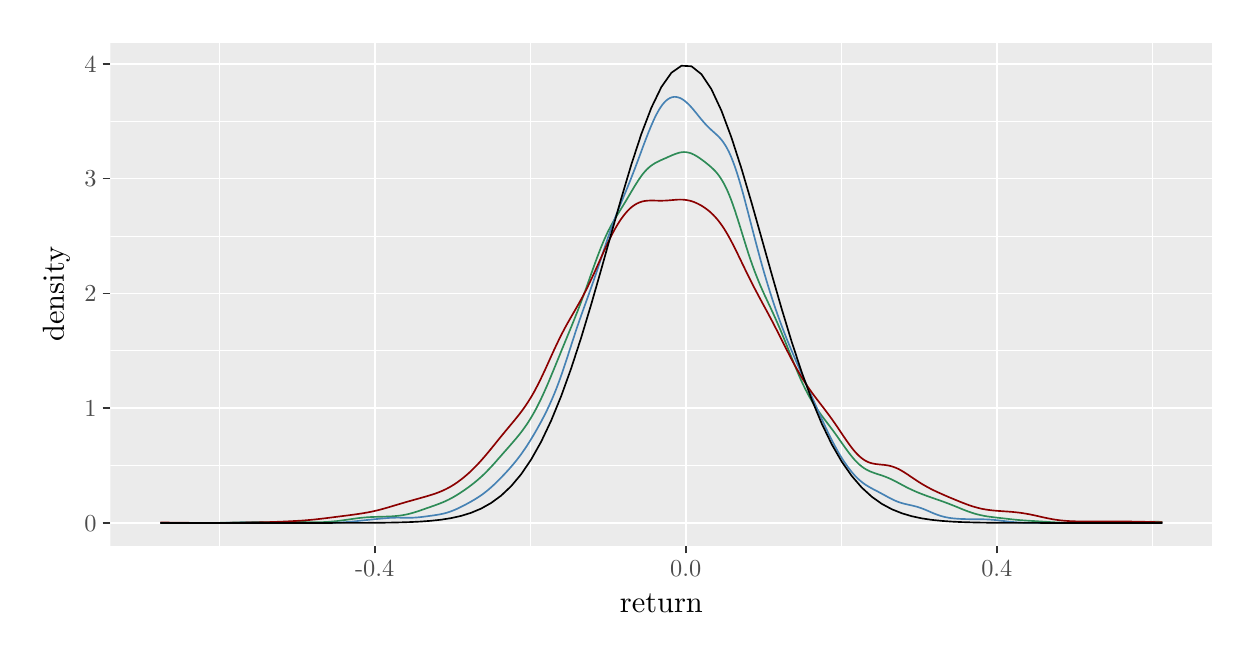
\begin{tikzpicture}[x=1pt,y=1pt]
\definecolor{fillColor}{RGB}{255,255,255}
\path[use as bounding box,fill=fillColor,fill opacity=0.00] (0,0) rectangle (433.62,216.81);
\begin{scope}
\path[clip] (  0.00,  0.00) rectangle (433.62,216.81);
\definecolor{drawColor}{RGB}{255,255,255}
\definecolor{fillColor}{RGB}{255,255,255}

\path[draw=drawColor,line width= 0.6pt,line join=round,line cap=round,fill=fillColor] (  0.00,  0.00) rectangle (433.62,216.81);
\end{scope}
\begin{scope}
\path[clip] ( 29.87, 29.59) rectangle (428.12,211.31);
\definecolor{fillColor}{gray}{0.92}

\path[fill=fillColor] ( 29.87, 29.59) rectangle (428.12,211.31);
\definecolor{drawColor}{RGB}{255,255,255}

\path[draw=drawColor,line width= 0.3pt,line join=round] ( 29.87, 58.58) --
	(428.12, 58.58);

\path[draw=drawColor,line width= 0.3pt,line join=round] ( 29.87,100.06) --
	(428.12,100.06);

\path[draw=drawColor,line width= 0.3pt,line join=round] ( 29.87,141.53) --
	(428.12,141.53);

\path[draw=drawColor,line width= 0.3pt,line join=round] ( 29.87,183.01) --
	(428.12,183.01);

\path[draw=drawColor,line width= 0.3pt,line join=round] ( 69.21, 29.59) --
	( 69.21,211.31);

\path[draw=drawColor,line width= 0.3pt,line join=round] (181.61, 29.59) --
	(181.61,211.31);

\path[draw=drawColor,line width= 0.3pt,line join=round] (294.01, 29.59) --
	(294.01,211.31);

\path[draw=drawColor,line width= 0.3pt,line join=round] (406.41, 29.59) --
	(406.41,211.31);

\path[draw=drawColor,line width= 0.6pt,line join=round] ( 29.87, 37.85) --
	(428.12, 37.85);

\path[draw=drawColor,line width= 0.6pt,line join=round] ( 29.87, 79.32) --
	(428.12, 79.32);

\path[draw=drawColor,line width= 0.6pt,line join=round] ( 29.87,120.80) --
	(428.12,120.80);

\path[draw=drawColor,line width= 0.6pt,line join=round] ( 29.87,162.27) --
	(428.12,162.27);

\path[draw=drawColor,line width= 0.6pt,line join=round] ( 29.87,203.75) --
	(428.12,203.75);

\path[draw=drawColor,line width= 0.6pt,line join=round] (125.41, 29.59) --
	(125.41,211.31);

\path[draw=drawColor,line width= 0.6pt,line join=round] (237.81, 29.59) --
	(237.81,211.31);

\path[draw=drawColor,line width= 0.6pt,line join=round] (350.21, 29.59) --
	(350.21,211.31);
\definecolor{drawColor}{RGB}{46,139,87}

\path[draw=drawColor,line width= 0.6pt,line join=round] ( 47.97, 37.85) --
	( 48.68, 37.85) --
	( 49.39, 37.85) --
	( 50.10, 37.85) --
	( 50.81, 37.85) --
	( 51.51, 37.85) --
	( 52.22, 37.85) --
	( 52.93, 37.85) --
	( 53.64, 37.85) --
	( 54.35, 37.85) --
	( 55.06, 37.85) --
	( 55.76, 37.85) --
	( 56.47, 37.85) --
	( 57.18, 37.85) --
	( 57.89, 37.85) --
	( 58.60, 37.85) --
	( 59.31, 37.85) --
	( 60.02, 37.85) --
	( 60.72, 37.85) --
	( 61.43, 37.85) --
	( 62.14, 37.85) --
	( 62.85, 37.85) --
	( 63.56, 37.85) --
	( 64.27, 37.85) --
	( 64.98, 37.85) --
	( 65.68, 37.85) --
	( 66.39, 37.86) --
	( 67.10, 37.86) --
	( 67.81, 37.86) --
	( 68.52, 37.87) --
	( 69.23, 37.88) --
	( 69.93, 37.89) --
	( 70.64, 37.90) --
	( 71.35, 37.91) --
	( 72.06, 37.92) --
	( 72.77, 37.94) --
	( 73.48, 37.96) --
	( 74.19, 37.98) --
	( 74.89, 38.00) --
	( 75.60, 38.02) --
	( 76.31, 38.05) --
	( 77.02, 38.07) --
	( 77.73, 38.09) --
	( 78.44, 38.11) --
	( 79.15, 38.13) --
	( 79.85, 38.14) --
	( 80.56, 38.15) --
	( 81.27, 38.16) --
	( 81.98, 38.17) --
	( 82.69, 38.17) --
	( 83.40, 38.17) --
	( 84.10, 38.16) --
	( 84.81, 38.16) --
	( 85.52, 38.15) --
	( 86.23, 38.14) --
	( 86.94, 38.13) --
	( 87.65, 38.12) --
	( 88.36, 38.12) --
	( 89.06, 38.12) --
	( 89.77, 38.12) --
	( 90.48, 38.12) --
	( 91.19, 38.13) --
	( 91.90, 38.14) --
	( 92.61, 38.15) --
	( 93.32, 38.16) --
	( 94.02, 38.17) --
	( 94.73, 38.18) --
	( 95.44, 38.19) --
	( 96.15, 38.19) --
	( 96.86, 38.19) --
	( 97.57, 38.19) --
	( 98.28, 38.19) --
	( 98.98, 38.18) --
	( 99.69, 38.17) --
	(100.40, 38.16) --
	(101.11, 38.14) --
	(101.82, 38.13) --
	(102.53, 38.12) --
	(103.23, 38.11) --
	(103.94, 38.11) --
	(104.65, 38.11) --
	(105.36, 38.12) --
	(106.07, 38.13) --
	(106.78, 38.15) --
	(107.49, 38.18) --
	(108.19, 38.22) --
	(108.90, 38.26) --
	(109.61, 38.32) --
	(110.32, 38.38) --
	(111.03, 38.45) --
	(111.74, 38.52) --
	(112.45, 38.61) --
	(113.15, 38.70) --
	(113.86, 38.79) --
	(114.57, 38.89) --
	(115.28, 38.99) --
	(115.99, 39.10) --
	(116.70, 39.20) --
	(117.40, 39.30) --
	(118.11, 39.40) --
	(118.82, 39.50) --
	(119.53, 39.59) --
	(120.24, 39.67) --
	(120.95, 39.74) --
	(121.66, 39.81) --
	(122.36, 39.87) --
	(123.07, 39.92) --
	(123.78, 39.96) --
	(124.49, 39.99) --
	(125.20, 40.02) --
	(125.91, 40.04) --
	(126.62, 40.06) --
	(127.32, 40.08) --
	(128.03, 40.10) --
	(128.74, 40.12) --
	(129.45, 40.14) --
	(130.16, 40.16) --
	(130.87, 40.20) --
	(131.57, 40.23) --
	(132.28, 40.28) --
	(132.99, 40.34) --
	(133.70, 40.41) --
	(134.41, 40.49) --
	(135.12, 40.59) --
	(135.83, 40.71) --
	(136.53, 40.84) --
	(137.24, 40.99) --
	(137.95, 41.16) --
	(138.66, 41.35) --
	(139.37, 41.55) --
	(140.08, 41.77) --
	(140.79, 41.99) --
	(141.49, 42.23) --
	(142.20, 42.47) --
	(142.91, 42.72) --
	(143.62, 42.97) --
	(144.33, 43.22) --
	(145.04, 43.46) --
	(145.74, 43.71) --
	(146.45, 43.96) --
	(147.16, 44.21) --
	(147.87, 44.47) --
	(148.58, 44.73) --
	(149.29, 45.01) --
	(150.00, 45.30) --
	(150.70, 45.60) --
	(151.41, 45.93) --
	(152.12, 46.27) --
	(152.83, 46.64) --
	(153.54, 47.02) --
	(154.25, 47.43) --
	(154.96, 47.85) --
	(155.66, 48.29) --
	(156.37, 48.74) --
	(157.08, 49.21) --
	(157.79, 49.70) --
	(158.50, 50.20) --
	(159.21, 50.71) --
	(159.92, 51.23) --
	(160.62, 51.77) --
	(161.33, 52.33) --
	(162.04, 52.91) --
	(162.75, 53.51) --
	(163.46, 54.13) --
	(164.17, 54.77) --
	(164.87, 55.44) --
	(165.58, 56.14) --
	(166.29, 56.87) --
	(167.00, 57.61) --
	(167.71, 58.37) --
	(168.42, 59.15) --
	(169.13, 59.94) --
	(169.83, 60.75) --
	(170.54, 61.55) --
	(171.25, 62.36) --
	(171.96, 63.17) --
	(172.67, 63.97) --
	(173.38, 64.78) --
	(174.09, 65.58) --
	(174.79, 66.39) --
	(175.50, 67.21) --
	(176.21, 68.04) --
	(176.92, 68.89) --
	(177.63, 69.76) --
	(178.34, 70.66) --
	(179.04, 71.61) --
	(179.75, 72.59) --
	(180.46, 73.63) --
	(181.17, 74.71) --
	(181.88, 75.86) --
	(182.59, 77.06) --
	(183.30, 78.32) --
	(184.00, 79.65) --
	(184.71, 81.05) --
	(185.42, 82.50) --
	(186.13, 84.02) --
	(186.84, 85.58) --
	(187.55, 87.19) --
	(188.26, 88.84) --
	(188.96, 90.53) --
	(189.67, 92.24) --
	(190.38, 93.96) --
	(191.09, 95.70) --
	(191.80, 97.44) --
	(192.51, 99.17) --
	(193.21,100.90) --
	(193.92,102.63) --
	(194.63,104.35) --
	(195.34,106.07) --
	(196.05,107.79) --
	(196.76,109.52) --
	(197.47,111.27) --
	(198.17,113.04) --
	(198.88,114.84) --
	(199.59,116.69) --
	(200.30,118.56) --
	(201.01,120.48) --
	(201.72,122.43) --
	(202.43,124.41) --
	(203.13,126.42) --
	(203.84,128.42) --
	(204.55,130.42) --
	(205.26,132.38) --
	(205.97,134.30) --
	(206.68,136.15) --
	(207.39,137.94) --
	(208.09,139.63) --
	(208.80,141.24) --
	(209.51,142.75) --
	(210.22,144.16) --
	(210.93,145.49) --
	(211.64,146.75) --
	(212.34,147.96) --
	(213.05,149.13) --
	(213.76,150.28) --
	(214.47,151.43) --
	(215.18,152.58) --
	(215.89,153.75) --
	(216.60,154.93) --
	(217.30,156.13) --
	(218.01,157.33) --
	(218.72,158.53) --
	(219.43,159.70) --
	(220.14,160.84) --
	(220.85,161.93) --
	(221.56,162.96) --
	(222.26,163.91) --
	(222.97,164.76) --
	(223.68,165.52) --
	(224.39,166.20) --
	(225.10,166.79) --
	(225.81,167.30) --
	(226.51,167.75) --
	(227.22,168.15) --
	(227.93,168.50) --
	(228.64,168.84) --
	(229.35,169.16) --
	(230.06,169.47) --
	(230.77,169.78) --
	(231.47,170.10) --
	(232.18,170.41) --
	(232.89,170.72) --
	(233.60,171.01) --
	(234.31,171.28) --
	(235.02,171.51) --
	(235.73,171.70) --
	(236.43,171.81) --
	(237.14,171.86) --
	(237.85,171.83) --
	(238.56,171.72) --
	(239.27,171.54) --
	(239.98,171.29) --
	(240.68,170.96) --
	(241.39,170.58) --
	(242.10,170.14) --
	(242.81,169.67) --
	(243.52,169.16) --
	(244.23,168.64) --
	(244.94,168.09) --
	(245.64,167.53) --
	(246.35,166.94) --
	(247.06,166.32) --
	(247.77,165.65) --
	(248.48,164.93) --
	(249.19,164.11) --
	(249.90,163.19) --
	(250.60,162.14) --
	(251.31,160.96) --
	(252.02,159.63) --
	(252.73,158.15) --
	(253.44,156.51) --
	(254.15,154.72) --
	(254.85,152.78) --
	(255.56,150.71) --
	(256.27,148.54) --
	(256.98,146.30) --
	(257.69,144.02) --
	(258.40,141.71) --
	(259.11,139.42) --
	(259.81,137.17) --
	(260.52,134.97) --
	(261.23,132.84) --
	(261.94,130.81) --
	(262.65,128.88) --
	(263.36,127.03) --
	(264.07,125.27) --
	(264.77,123.59) --
	(265.48,121.97) --
	(266.19,120.40) --
	(266.90,118.87) --
	(267.61,117.35) --
	(268.32,115.84) --
	(269.03,114.31) --
	(269.73,112.76) --
	(270.44,111.18) --
	(271.15,109.56) --
	(271.86,107.91) --
	(272.57,106.22) --
	(273.28,104.49) --
	(273.98,102.74) --
	(274.69,100.97) --
	(275.40, 99.20) --
	(276.11, 97.43) --
	(276.82, 95.67) --
	(277.53, 93.95) --
	(278.24, 92.26) --
	(278.94, 90.62) --
	(279.65, 89.04) --
	(280.36, 87.52) --
	(281.07, 86.07) --
	(281.78, 84.70) --
	(282.49, 83.40) --
	(283.20, 82.17) --
	(283.90, 81.01) --
	(284.61, 79.91) --
	(285.32, 78.85) --
	(286.03, 77.85) --
	(286.74, 76.87) --
	(287.45, 75.93) --
	(288.15, 74.99) --
	(288.86, 74.06) --
	(289.57, 73.13) --
	(290.28, 72.19) --
	(290.99, 71.23) --
	(291.70, 70.26) --
	(292.41, 69.27) --
	(293.11, 68.27) --
	(293.82, 67.26) --
	(294.53, 66.25) --
	(295.24, 65.25) --
	(295.95, 64.27) --
	(296.66, 63.31) --
	(297.37, 62.39) --
	(298.07, 61.52) --
	(298.78, 60.69) --
	(299.49, 59.93) --
	(300.20, 59.24) --
	(300.91, 58.62) --
	(301.62, 58.07) --
	(302.32, 57.58) --
	(303.03, 57.15) --
	(303.74, 56.78) --
	(304.45, 56.45) --
	(305.16, 56.17) --
	(305.87, 55.91) --
	(306.58, 55.67) --
	(307.28, 55.44) --
	(307.99, 55.21) --
	(308.70, 54.98) --
	(309.41, 54.73) --
	(310.12, 54.46) --
	(310.83, 54.17) --
	(311.54, 53.86) --
	(312.24, 53.53) --
	(312.95, 53.18) --
	(313.66, 52.82) --
	(314.37, 52.45) --
	(315.08, 52.07) --
	(315.79, 51.69) --
	(316.49, 51.31) --
	(317.20, 50.94) --
	(317.91, 50.58) --
	(318.62, 50.23) --
	(319.33, 49.89) --
	(320.04, 49.57) --
	(320.75, 49.25) --
	(321.45, 48.95) --
	(322.16, 48.66) --
	(322.87, 48.38) --
	(323.58, 48.11) --
	(324.29, 47.84) --
	(325.00, 47.58) --
	(325.71, 47.33) --
	(326.41, 47.08) --
	(327.12, 46.83) --
	(327.83, 46.58) --
	(328.54, 46.34) --
	(329.25, 46.09) --
	(329.96, 45.84) --
	(330.67, 45.59) --
	(331.37, 45.33) --
	(332.08, 45.07) --
	(332.79, 44.80) --
	(333.50, 44.52) --
	(334.21, 44.24) --
	(334.92, 43.96) --
	(335.62, 43.67) --
	(336.33, 43.38) --
	(337.04, 43.09) --
	(337.75, 42.80) --
	(338.46, 42.52) --
	(339.17, 42.24) --
	(339.88, 41.98) --
	(340.58, 41.73) --
	(341.29, 41.49) --
	(342.00, 41.27) --
	(342.71, 41.06) --
	(343.42, 40.88) --
	(344.13, 40.71) --
	(344.84, 40.55) --
	(345.54, 40.42) --
	(346.25, 40.29) --
	(346.96, 40.18) --
	(347.67, 40.08) --
	(348.38, 39.99) --
	(349.09, 39.90) --
	(349.79, 39.82) --
	(350.50, 39.73) --
	(351.21, 39.65) --
	(351.92, 39.57) --
	(352.63, 39.49) --
	(353.34, 39.41) --
	(354.05, 39.33) --
	(354.75, 39.25) --
	(355.46, 39.17) --
	(356.17, 39.09) --
	(356.88, 39.02) --
	(357.59, 38.95) --
	(358.30, 38.89) --
	(359.01, 38.83) --
	(359.71, 38.78) --
	(360.42, 38.73) --
	(361.13, 38.68) --
	(361.84, 38.64) --
	(362.55, 38.59) --
	(363.26, 38.55) --
	(363.96, 38.51) --
	(364.67, 38.47) --
	(365.38, 38.42) --
	(366.09, 38.38) --
	(366.80, 38.33) --
	(367.51, 38.29) --
	(368.22, 38.24) --
	(368.92, 38.19) --
	(369.63, 38.15) --
	(370.34, 38.11) --
	(371.05, 38.07) --
	(371.76, 38.03) --
	(372.47, 38.00) --
	(373.18, 37.97) --
	(373.88, 37.95) --
	(374.59, 37.92) --
	(375.30, 37.91) --
	(376.01, 37.89) --
	(376.72, 37.88) --
	(377.43, 37.87) --
	(378.13, 37.87) --
	(378.84, 37.86) --
	(379.55, 37.86) --
	(380.26, 37.85) --
	(380.97, 37.85) --
	(381.68, 37.85) --
	(382.39, 37.85) --
	(383.09, 37.85) --
	(383.80, 37.85) --
	(384.51, 37.85) --
	(385.22, 37.85) --
	(385.93, 37.85) --
	(386.64, 37.85) --
	(387.35, 37.85) --
	(388.05, 37.86) --
	(388.76, 37.86) --
	(389.47, 37.86) --
	(390.18, 37.87) --
	(390.89, 37.88) --
	(391.60, 37.88) --
	(392.31, 37.89) --
	(393.01, 37.91) --
	(393.72, 37.92) --
	(394.43, 37.93) --
	(395.14, 37.95) --
	(395.85, 37.97) --
	(396.56, 37.99) --
	(397.26, 38.01) --
	(397.97, 38.03) --
	(398.68, 38.05) --
	(399.39, 38.08) --
	(400.10, 38.10) --
	(400.81, 38.12) --
	(401.52, 38.15) --
	(402.22, 38.17) --
	(402.93, 38.19) --
	(403.64, 38.21) --
	(404.35, 38.22) --
	(405.06, 38.24) --
	(405.77, 38.25) --
	(406.48, 38.25) --
	(407.18, 38.26) --
	(407.89, 38.25) --
	(408.60, 38.25) --
	(409.31, 38.24) --
	(410.02, 38.22);
\definecolor{drawColor}{RGB}{70,130,180}

\path[draw=drawColor,line width= 0.6pt,line join=round] ( 47.97, 37.85) --
	( 48.68, 37.85) --
	( 49.39, 37.85) --
	( 50.10, 37.85) --
	( 50.81, 37.85) --
	( 51.51, 37.85) --
	( 52.22, 37.85) --
	( 52.93, 37.85) --
	( 53.64, 37.85) --
	( 54.35, 37.85) --
	( 55.06, 37.85) --
	( 55.76, 37.85) --
	( 56.47, 37.85) --
	( 57.18, 37.85) --
	( 57.89, 37.85) --
	( 58.60, 37.85) --
	( 59.31, 37.85) --
	( 60.02, 37.85) --
	( 60.72, 37.85) --
	( 61.43, 37.85) --
	( 62.14, 37.85) --
	( 62.85, 37.85) --
	( 63.56, 37.85) --
	( 64.27, 37.85) --
	( 64.98, 37.85) --
	( 65.68, 37.85) --
	( 66.39, 37.85) --
	( 67.10, 37.85) --
	( 67.81, 37.85) --
	( 68.52, 37.86) --
	( 69.23, 37.86) --
	( 69.93, 37.86) --
	( 70.64, 37.87) --
	( 71.35, 37.88) --
	( 72.06, 37.89) --
	( 72.77, 37.90) --
	( 73.48, 37.91) --
	( 74.19, 37.93) --
	( 74.89, 37.94) --
	( 75.60, 37.96) --
	( 76.31, 37.97) --
	( 77.02, 37.99) --
	( 77.73, 38.00) --
	( 78.44, 38.02) --
	( 79.15, 38.02) --
	( 79.85, 38.03) --
	( 80.56, 38.03) --
	( 81.27, 38.03) --
	( 81.98, 38.03) --
	( 82.69, 38.02) --
	( 83.40, 38.01) --
	( 84.10, 38.00) --
	( 84.81, 37.98) --
	( 85.52, 37.96) --
	( 86.23, 37.95) --
	( 86.94, 37.93) --
	( 87.65, 37.92) --
	( 88.36, 37.90) --
	( 89.06, 37.89) --
	( 89.77, 37.88) --
	( 90.48, 37.87) --
	( 91.19, 37.87) --
	( 91.90, 37.86) --
	( 92.61, 37.86) --
	( 93.32, 37.85) --
	( 94.02, 37.85) --
	( 94.73, 37.85) --
	( 95.44, 37.85) --
	( 96.15, 37.85) --
	( 96.86, 37.85) --
	( 97.57, 37.85) --
	( 98.28, 37.85) --
	( 98.98, 37.85) --
	( 99.69, 37.85) --
	(100.40, 37.85) --
	(101.11, 37.85) --
	(101.82, 37.85) --
	(102.53, 37.85) --
	(103.23, 37.85) --
	(103.94, 37.85) --
	(104.65, 37.85) --
	(105.36, 37.85) --
	(106.07, 37.85) --
	(106.78, 37.86) --
	(107.49, 37.86) --
	(108.19, 37.87) --
	(108.90, 37.88) --
	(109.61, 37.89) --
	(110.32, 37.91) --
	(111.03, 37.93) --
	(111.74, 37.96) --
	(112.45, 37.99) --
	(113.15, 38.02) --
	(113.86, 38.06) --
	(114.57, 38.11) --
	(115.28, 38.17) --
	(115.99, 38.23) --
	(116.70, 38.29) --
	(117.40, 38.36) --
	(118.11, 38.43) --
	(118.82, 38.50) --
	(119.53, 38.58) --
	(120.24, 38.66) --
	(120.95, 38.73) --
	(121.66, 38.81) --
	(122.36, 38.88) --
	(123.07, 38.95) --
	(123.78, 39.03) --
	(124.49, 39.10) --
	(125.20, 39.17) --
	(125.91, 39.24) --
	(126.62, 39.31) --
	(127.32, 39.38) --
	(128.03, 39.44) --
	(128.74, 39.51) --
	(129.45, 39.57) --
	(130.16, 39.62) --
	(130.87, 39.67) --
	(131.57, 39.70) --
	(132.28, 39.73) --
	(132.99, 39.75) --
	(133.70, 39.75) --
	(134.41, 39.75) --
	(135.12, 39.74) --
	(135.83, 39.73) --
	(136.53, 39.72) --
	(137.24, 39.71) --
	(137.95, 39.71) --
	(138.66, 39.73) --
	(139.37, 39.75) --
	(140.08, 39.79) --
	(140.79, 39.84) --
	(141.49, 39.91) --
	(142.20, 39.98) --
	(142.91, 40.07) --
	(143.62, 40.16) --
	(144.33, 40.25) --
	(145.04, 40.35) --
	(145.74, 40.45) --
	(146.45, 40.54) --
	(147.16, 40.65) --
	(147.87, 40.76) --
	(148.58, 40.88) --
	(149.29, 41.01) --
	(150.00, 41.16) --
	(150.70, 41.33) --
	(151.41, 41.53) --
	(152.12, 41.74) --
	(152.83, 41.99) --
	(153.54, 42.26) --
	(154.25, 42.55) --
	(154.96, 42.86) --
	(155.66, 43.19) --
	(156.37, 43.53) --
	(157.08, 43.89) --
	(157.79, 44.25) --
	(158.50, 44.63) --
	(159.21, 45.01) --
	(159.92, 45.40) --
	(160.62, 45.81) --
	(161.33, 46.22) --
	(162.04, 46.65) --
	(162.75, 47.10) --
	(163.46, 47.57) --
	(164.17, 48.06) --
	(164.87, 48.58) --
	(165.58, 49.13) --
	(166.29, 49.70) --
	(167.00, 50.31) --
	(167.71, 50.94) --
	(168.42, 51.59) --
	(169.13, 52.27) --
	(169.83, 52.96) --
	(170.54, 53.67) --
	(171.25, 54.40) --
	(171.96, 55.14) --
	(172.67, 55.89) --
	(173.38, 56.66) --
	(174.09, 57.45) --
	(174.79, 58.26) --
	(175.50, 59.09) --
	(176.21, 59.95) --
	(176.92, 60.84) --
	(177.63, 61.76) --
	(178.34, 62.72) --
	(179.04, 63.72) --
	(179.75, 64.75) --
	(180.46, 65.82) --
	(181.17, 66.93) --
	(181.88, 68.07) --
	(182.59, 69.24) --
	(183.30, 70.44) --
	(184.00, 71.67) --
	(184.71, 72.94) --
	(185.42, 74.23) --
	(186.13, 75.57) --
	(186.84, 76.95) --
	(187.55, 78.38) --
	(188.26, 79.87) --
	(188.96, 81.42) --
	(189.67, 83.03) --
	(190.38, 84.73) --
	(191.09, 86.51) --
	(191.80, 88.37) --
	(192.51, 90.32) --
	(193.21, 92.34) --
	(193.92, 94.44) --
	(194.63, 96.59) --
	(195.34, 98.77) --
	(196.05,100.96) --
	(196.76,103.15) --
	(197.47,105.33) --
	(198.17,107.47) --
	(198.88,109.57) --
	(199.59,111.62) --
	(200.30,113.64) --
	(201.01,115.62) --
	(201.72,117.58) --
	(202.43,119.55) --
	(203.13,121.52) --
	(203.84,123.52) --
	(204.55,125.55) --
	(205.26,127.62) --
	(205.97,129.72) --
	(206.68,131.86) --
	(207.39,134.01) --
	(208.09,136.16) --
	(208.80,138.30) --
	(209.51,140.41) --
	(210.22,142.47) --
	(210.93,144.47) --
	(211.64,146.42) --
	(212.34,148.30) --
	(213.05,150.12) --
	(213.76,151.89) --
	(214.47,153.62) --
	(215.18,155.34) --
	(215.89,157.05) --
	(216.60,158.77) --
	(217.30,160.52) --
	(218.01,162.29) --
	(218.72,164.11) --
	(219.43,165.95) --
	(220.14,167.83) --
	(220.85,169.74) --
	(221.56,171.65) --
	(222.26,173.57) --
	(222.97,175.46) --
	(223.68,177.32) --
	(224.39,179.13) --
	(225.10,180.86) --
	(225.81,182.51) --
	(226.51,184.06) --
	(227.22,185.49) --
	(227.93,186.79) --
	(228.64,187.96) --
	(229.35,188.96) --
	(230.06,189.81) --
	(230.77,190.50) --
	(231.47,191.04) --
	(232.18,191.43) --
	(232.89,191.68) --
	(233.60,191.80) --
	(234.31,191.78) --
	(235.02,191.64) --
	(235.73,191.39) --
	(236.43,191.03) --
	(237.14,190.56) --
	(237.85,190.00) --
	(238.56,189.35) --
	(239.27,188.64) --
	(239.98,187.86) --
	(240.68,187.04) --
	(241.39,186.18) --
	(242.10,185.30) --
	(242.81,184.42) --
	(243.52,183.55) --
	(244.23,182.72) --
	(244.94,181.93) --
	(245.64,181.19) --
	(246.35,180.49) --
	(247.06,179.83) --
	(247.77,179.19) --
	(248.48,178.55) --
	(249.19,177.90) --
	(249.90,177.19) --
	(250.60,176.40) --
	(251.31,175.49) --
	(252.02,174.43) --
	(252.73,173.21) --
	(253.44,171.82) --
	(254.15,170.24) --
	(254.85,168.48) --
	(255.56,166.54) --
	(256.27,164.42) --
	(256.98,162.16) --
	(257.69,159.75) --
	(258.40,157.22) --
	(259.11,154.60) --
	(259.81,151.92) --
	(260.52,149.20) --
	(261.23,146.46) --
	(261.94,143.72) --
	(262.65,140.99) --
	(263.36,138.30) --
	(264.07,135.65) --
	(264.77,133.05) --
	(265.48,130.51) --
	(266.19,128.04) --
	(266.90,125.64) --
	(267.61,123.30) --
	(268.32,121.04) --
	(269.03,118.84) --
	(269.73,116.70) --
	(270.44,114.63) --
	(271.15,112.61) --
	(271.86,110.66) --
	(272.57,108.76) --
	(273.28,106.91) --
	(273.98,105.11) --
	(274.69,103.35) --
	(275.40,101.63) --
	(276.11, 99.94) --
	(276.82, 98.27) --
	(277.53, 96.63) --
	(278.24, 95.00) --
	(278.94, 93.39) --
	(279.65, 91.80) --
	(280.36, 90.20) --
	(281.07, 88.61) --
	(281.78, 87.02) --
	(282.49, 85.43) --
	(283.20, 83.83) --
	(283.90, 82.24) --
	(284.61, 80.64) --
	(285.32, 79.04) --
	(286.03, 77.44) --
	(286.74, 75.86) --
	(287.45, 74.30) --
	(288.15, 72.76) --
	(288.86, 71.25) --
	(289.57, 69.78) --
	(290.28, 68.35) --
	(290.99, 66.96) --
	(291.70, 65.62) --
	(292.41, 64.32) --
	(293.11, 63.08) --
	(293.82, 61.89) --
	(294.53, 60.76) --
	(295.24, 59.68) --
	(295.95, 58.65) --
	(296.66, 57.68) --
	(297.37, 56.76) --
	(298.07, 55.90) --
	(298.78, 55.10) --
	(299.49, 54.35) --
	(300.20, 53.67) --
	(300.91, 53.04) --
	(301.62, 52.47) --
	(302.32, 51.95) --
	(303.03, 51.47) --
	(303.74, 51.04) --
	(304.45, 50.63) --
	(305.16, 50.24) --
	(305.87, 49.86) --
	(306.58, 49.49) --
	(307.28, 49.13) --
	(307.99, 48.75) --
	(308.70, 48.37) --
	(309.41, 47.99) --
	(310.12, 47.60) --
	(310.83, 47.21) --
	(311.54, 46.84) --
	(312.24, 46.47) --
	(312.95, 46.13) --
	(313.66, 45.81) --
	(314.37, 45.52) --
	(315.08, 45.27) --
	(315.79, 45.04) --
	(316.49, 44.85) --
	(317.20, 44.67) --
	(317.91, 44.51) --
	(318.62, 44.35) --
	(319.33, 44.20) --
	(320.04, 44.03) --
	(320.75, 43.85) --
	(321.45, 43.66) --
	(322.16, 43.43) --
	(322.87, 43.19) --
	(323.58, 42.92) --
	(324.29, 42.63) --
	(325.00, 42.34) --
	(325.71, 42.03) --
	(326.41, 41.72) --
	(327.12, 41.42) --
	(327.83, 41.13) --
	(328.54, 40.86) --
	(329.25, 40.61) --
	(329.96, 40.38) --
	(330.67, 40.18) --
	(331.37, 40.00) --
	(332.08, 39.85) --
	(332.79, 39.72) --
	(333.50, 39.61) --
	(334.21, 39.52) --
	(334.92, 39.45) --
	(335.62, 39.39) --
	(336.33, 39.34) --
	(337.04, 39.30) --
	(337.75, 39.27) --
	(338.46, 39.25) --
	(339.17, 39.23) --
	(339.88, 39.21) --
	(340.58, 39.20) --
	(341.29, 39.19) --
	(342.00, 39.19) --
	(342.71, 39.19) --
	(343.42, 39.18) --
	(344.13, 39.18) --
	(344.84, 39.17) --
	(345.54, 39.15) --
	(346.25, 39.13) --
	(346.96, 39.10) --
	(347.67, 39.06) --
	(348.38, 39.01) --
	(349.09, 38.95) --
	(349.79, 38.88) --
	(350.50, 38.81) --
	(351.21, 38.73) --
	(351.92, 38.64) --
	(352.63, 38.56) --
	(353.34, 38.47) --
	(354.05, 38.39) --
	(354.75, 38.31) --
	(355.46, 38.23) --
	(356.17, 38.17) --
	(356.88, 38.11) --
	(357.59, 38.05) --
	(358.30, 38.01) --
	(359.01, 37.97) --
	(359.71, 37.94) --
	(360.42, 37.92) --
	(361.13, 37.90) --
	(361.84, 37.89) --
	(362.55, 37.87) --
	(363.26, 37.87) --
	(363.96, 37.86) --
	(364.67, 37.86) --
	(365.38, 37.85) --
	(366.09, 37.85) --
	(366.80, 37.85) --
	(367.51, 37.85) --
	(368.22, 37.85) --
	(368.92, 37.85) --
	(369.63, 37.85) --
	(370.34, 37.85) --
	(371.05, 37.85) --
	(371.76, 37.85) --
	(372.47, 37.85) --
	(373.18, 37.85) --
	(373.88, 37.85) --
	(374.59, 37.85) --
	(375.30, 37.85) --
	(376.01, 37.85) --
	(376.72, 37.86) --
	(377.43, 37.86) --
	(378.13, 37.86) --
	(378.84, 37.87) --
	(379.55, 37.88) --
	(380.26, 37.88) --
	(380.97, 37.90) --
	(381.68, 37.91) --
	(382.39, 37.92) --
	(383.09, 37.94) --
	(383.80, 37.95) --
	(384.51, 37.97) --
	(385.22, 37.98) --
	(385.93, 38.00) --
	(386.64, 38.01) --
	(387.35, 38.02) --
	(388.05, 38.03) --
	(388.76, 38.03) --
	(389.47, 38.03) --
	(390.18, 38.03) --
	(390.89, 38.02) --
	(391.60, 38.01) --
	(392.31, 38.00) --
	(393.01, 37.99) --
	(393.72, 37.97) --
	(394.43, 37.95) --
	(395.14, 37.94) --
	(395.85, 37.92) --
	(396.56, 37.91) --
	(397.26, 37.90) --
	(397.97, 37.89) --
	(398.68, 37.88) --
	(399.39, 37.87) --
	(400.10, 37.86) --
	(400.81, 37.86) --
	(401.52, 37.86) --
	(402.22, 37.85) --
	(402.93, 37.85) --
	(403.64, 37.85) --
	(404.35, 37.85) --
	(405.06, 37.85) --
	(405.77, 37.85) --
	(406.48, 37.85) --
	(407.18, 37.85) --
	(407.89, 37.85) --
	(408.60, 37.85) --
	(409.31, 37.85) --
	(410.02, 37.85);
\definecolor{drawColor}{RGB}{139,0,0}

\path[draw=drawColor,line width= 0.6pt,line join=round] ( 47.97, 37.99) --
	( 48.68, 37.99) --
	( 49.39, 37.99) --
	( 50.10, 37.99) --
	( 50.81, 37.98) --
	( 51.51, 37.97) --
	( 52.22, 37.96) --
	( 52.93, 37.95) --
	( 53.64, 37.95) --
	( 54.35, 37.94) --
	( 55.06, 37.93) --
	( 55.76, 37.92) --
	( 56.47, 37.91) --
	( 57.18, 37.90) --
	( 57.89, 37.89) --
	( 58.60, 37.88) --
	( 59.31, 37.88) --
	( 60.02, 37.87) --
	( 60.72, 37.87) --
	( 61.43, 37.86) --
	( 62.14, 37.86) --
	( 62.85, 37.86) --
	( 63.56, 37.86) --
	( 64.27, 37.85) --
	( 64.98, 37.85) --
	( 65.68, 37.85) --
	( 66.39, 37.85) --
	( 67.10, 37.85) --
	( 67.81, 37.86) --
	( 68.52, 37.86) --
	( 69.23, 37.86) --
	( 69.93, 37.86) --
	( 70.64, 37.87) --
	( 71.35, 37.87) --
	( 72.06, 37.88) --
	( 72.77, 37.88) --
	( 73.48, 37.89) --
	( 74.19, 37.90) --
	( 74.89, 37.91) --
	( 75.60, 37.92) --
	( 76.31, 37.93) --
	( 77.02, 37.94) --
	( 77.73, 37.95) --
	( 78.44, 37.97) --
	( 79.15, 37.98) --
	( 79.85, 37.99) --
	( 80.56, 38.01) --
	( 81.27, 38.02) --
	( 81.98, 38.03) --
	( 82.69, 38.05) --
	( 83.40, 38.06) --
	( 84.10, 38.07) --
	( 84.81, 38.09) --
	( 85.52, 38.11) --
	( 86.23, 38.12) --
	( 86.94, 38.14) --
	( 87.65, 38.16) --
	( 88.36, 38.18) --
	( 89.06, 38.21) --
	( 89.77, 38.23) --
	( 90.48, 38.26) --
	( 91.19, 38.29) --
	( 91.90, 38.32) --
	( 92.61, 38.35) --
	( 93.32, 38.38) --
	( 94.02, 38.42) --
	( 94.73, 38.45) --
	( 95.44, 38.49) --
	( 96.15, 38.53) --
	( 96.86, 38.56) --
	( 97.57, 38.61) --
	( 98.28, 38.65) --
	( 98.98, 38.69) --
	( 99.69, 38.74) --
	(100.40, 38.80) --
	(101.11, 38.85) --
	(101.82, 38.92) --
	(102.53, 38.98) --
	(103.23, 39.05) --
	(103.94, 39.12) --
	(104.65, 39.20) --
	(105.36, 39.28) --
	(106.07, 39.36) --
	(106.78, 39.45) --
	(107.49, 39.53) --
	(108.19, 39.62) --
	(108.90, 39.71) --
	(109.61, 39.80) --
	(110.32, 39.89) --
	(111.03, 39.98) --
	(111.74, 40.07) --
	(112.45, 40.16) --
	(113.15, 40.25) --
	(113.86, 40.34) --
	(114.57, 40.43) --
	(115.28, 40.52) --
	(115.99, 40.61) --
	(116.70, 40.71) --
	(117.40, 40.80) --
	(118.11, 40.90) --
	(118.82, 41.00) --
	(119.53, 41.10) --
	(120.24, 41.21) --
	(120.95, 41.32) --
	(121.66, 41.44) --
	(122.36, 41.56) --
	(123.07, 41.69) --
	(123.78, 41.83) --
	(124.49, 41.97) --
	(125.20, 42.13) --
	(125.91, 42.29) --
	(126.62, 42.46) --
	(127.32, 42.64) --
	(128.03, 42.83) --
	(128.74, 43.03) --
	(129.45, 43.23) --
	(130.16, 43.43) --
	(130.87, 43.64) --
	(131.57, 43.85) --
	(132.28, 44.07) --
	(132.99, 44.28) --
	(133.70, 44.49) --
	(134.41, 44.70) --
	(135.12, 44.91) --
	(135.83, 45.12) --
	(136.53, 45.33) --
	(137.24, 45.53) --
	(137.95, 45.73) --
	(138.66, 45.93) --
	(139.37, 46.13) --
	(140.08, 46.33) --
	(140.79, 46.52) --
	(141.49, 46.72) --
	(142.20, 46.92) --
	(142.91, 47.12) --
	(143.62, 47.32) --
	(144.33, 47.53) --
	(145.04, 47.74) --
	(145.74, 47.96) --
	(146.45, 48.18) --
	(147.16, 48.42) --
	(147.87, 48.67) --
	(148.58, 48.94) --
	(149.29, 49.23) --
	(150.00, 49.53) --
	(150.70, 49.86) --
	(151.41, 50.21) --
	(152.12, 50.58) --
	(152.83, 50.98) --
	(153.54, 51.40) --
	(154.25, 51.85) --
	(154.96, 52.32) --
	(155.66, 52.83) --
	(156.37, 53.35) --
	(157.08, 53.90) --
	(157.79, 54.48) --
	(158.50, 55.08) --
	(159.21, 55.70) --
	(159.92, 56.35) --
	(160.62, 57.03) --
	(161.33, 57.73) --
	(162.04, 58.45) --
	(162.75, 59.19) --
	(163.46, 59.96) --
	(164.17, 60.75) --
	(164.87, 61.56) --
	(165.58, 62.39) --
	(166.29, 63.23) --
	(167.00, 64.09) --
	(167.71, 64.96) --
	(168.42, 65.83) --
	(169.13, 66.71) --
	(169.83, 67.59) --
	(170.54, 68.46) --
	(171.25, 69.33) --
	(171.96, 70.19) --
	(172.67, 71.05) --
	(173.38, 71.90) --
	(174.09, 72.75) --
	(174.79, 73.60) --
	(175.50, 74.45) --
	(176.21, 75.31) --
	(176.92, 76.19) --
	(177.63, 77.08) --
	(178.34, 78.01) --
	(179.04, 78.97) --
	(179.75, 79.97) --
	(180.46, 81.02) --
	(181.17, 82.12) --
	(181.88, 83.27) --
	(182.59, 84.48) --
	(183.30, 85.76) --
	(184.00, 87.10) --
	(184.71, 88.49) --
	(185.42, 89.93) --
	(186.13, 91.42) --
	(186.84, 92.94) --
	(187.55, 94.49) --
	(188.26, 96.05) --
	(188.96, 97.62) --
	(189.67, 99.18) --
	(190.38,100.72) --
	(191.09,102.23) --
	(191.80,103.71) --
	(192.51,105.15) --
	(193.21,106.54) --
	(193.92,107.90) --
	(194.63,109.21) --
	(195.34,110.48) --
	(196.05,111.72) --
	(196.76,112.95) --
	(197.47,114.17) --
	(198.17,115.39) --
	(198.88,116.63) --
	(199.59,117.89) --
	(200.30,119.18) --
	(201.01,120.52) --
	(201.72,121.90) --
	(202.43,123.32) --
	(203.13,124.78) --
	(203.84,126.29) --
	(204.55,127.82) --
	(205.26,129.39) --
	(205.97,130.97) --
	(206.68,132.56) --
	(207.39,134.15) --
	(208.09,135.72) --
	(208.80,137.26) --
	(209.51,138.77) --
	(210.22,140.24) --
	(210.93,141.65) --
	(211.64,143.01) --
	(212.34,144.29) --
	(213.05,145.50) --
	(213.76,146.64) --
	(214.47,147.70) --
	(215.18,148.68) --
	(215.89,149.58) --
	(216.60,150.40) --
	(217.30,151.14) --
	(218.01,151.79) --
	(218.72,152.35) --
	(219.43,152.83) --
	(220.14,153.24) --
	(220.85,153.57) --
	(221.56,153.84) --
	(222.26,154.04) --
	(222.97,154.18) --
	(223.68,154.27) --
	(224.39,154.32) --
	(225.10,154.34) --
	(225.81,154.34) --
	(226.51,154.33) --
	(227.22,154.31) --
	(227.93,154.29) --
	(228.64,154.28) --
	(229.35,154.29) --
	(230.06,154.31) --
	(230.77,154.34) --
	(231.47,154.39) --
	(232.18,154.45) --
	(232.89,154.51) --
	(233.60,154.57) --
	(234.31,154.63) --
	(235.02,154.67) --
	(235.73,154.69) --
	(236.43,154.68) --
	(237.14,154.63) --
	(237.85,154.55) --
	(238.56,154.44) --
	(239.27,154.28) --
	(239.98,154.08) --
	(240.68,153.84) --
	(241.39,153.55) --
	(242.10,153.22) --
	(242.81,152.86) --
	(243.52,152.46) --
	(244.23,152.02) --
	(244.94,151.53) --
	(245.64,151.01) --
	(246.35,150.44) --
	(247.06,149.80) --
	(247.77,149.11) --
	(248.48,148.36) --
	(249.19,147.55) --
	(249.90,146.66) --
	(250.60,145.70) --
	(251.31,144.68) --
	(252.02,143.57) --
	(252.73,142.39) --
	(253.44,141.14) --
	(254.15,139.83) --
	(254.85,138.47) --
	(255.56,137.07) --
	(256.27,135.63) --
	(256.98,134.17) --
	(257.69,132.70) --
	(258.40,131.22) --
	(259.11,129.75) --
	(259.81,128.29) --
	(260.52,126.85) --
	(261.23,125.43) --
	(261.94,124.03) --
	(262.65,122.66) --
	(263.36,121.31) --
	(264.07,119.97) --
	(264.77,118.66) --
	(265.48,117.34) --
	(266.19,116.03) --
	(266.90,114.72) --
	(267.61,113.40) --
	(268.32,112.07) --
	(269.03,110.73) --
	(269.73,109.37) --
	(270.44,107.99) --
	(271.15,106.60) --
	(271.86,105.19) --
	(272.57,103.79) --
	(273.28,102.38) --
	(273.98,100.97) --
	(274.69, 99.57) --
	(275.40, 98.19) --
	(276.11, 96.84) --
	(276.82, 95.51) --
	(277.53, 94.21) --
	(278.24, 92.95) --
	(278.94, 91.73) --
	(279.65, 90.54) --
	(280.36, 89.39) --
	(281.07, 88.29) --
	(281.78, 87.23) --
	(282.49, 86.20) --
	(283.20, 85.20) --
	(283.90, 84.23) --
	(284.61, 83.28) --
	(285.32, 82.35) --
	(286.03, 81.43) --
	(286.74, 80.51) --
	(287.45, 79.59) --
	(288.15, 78.66) --
	(288.86, 77.72) --
	(289.57, 76.77) --
	(290.28, 75.79) --
	(290.99, 74.80) --
	(291.70, 73.79) --
	(292.41, 72.75) --
	(293.11, 71.71) --
	(293.82, 70.65) --
	(294.53, 69.60) --
	(295.24, 68.55) --
	(295.95, 67.52) --
	(296.66, 66.52) --
	(297.37, 65.55) --
	(298.07, 64.63) --
	(298.78, 63.78) --
	(299.49, 62.99) --
	(300.20, 62.27) --
	(300.91, 61.62) --
	(301.62, 61.06) --
	(302.32, 60.57) --
	(303.03, 60.16) --
	(303.74, 59.83) --
	(304.45, 59.57) --
	(305.16, 59.37) --
	(305.87, 59.22) --
	(306.58, 59.11) --
	(307.28, 59.03) --
	(307.99, 58.96) --
	(308.70, 58.89) --
	(309.41, 58.83) --
	(310.12, 58.74) --
	(310.83, 58.62) --
	(311.54, 58.47) --
	(312.24, 58.28) --
	(312.95, 58.05) --
	(313.66, 57.78) --
	(314.37, 57.47) --
	(315.08, 57.11) --
	(315.79, 56.72) --
	(316.49, 56.30) --
	(317.20, 55.85) --
	(317.91, 55.39) --
	(318.62, 54.91) --
	(319.33, 54.43) --
	(320.04, 53.95) --
	(320.75, 53.47) --
	(321.45, 53.00) --
	(322.16, 52.55) --
	(322.87, 52.11) --
	(323.58, 51.68) --
	(324.29, 51.27) --
	(325.00, 50.87) --
	(325.71, 50.49) --
	(326.41, 50.12) --
	(327.12, 49.77) --
	(327.83, 49.42) --
	(328.54, 49.09) --
	(329.25, 48.76) --
	(329.96, 48.45) --
	(330.67, 48.13) --
	(331.37, 47.82) --
	(332.08, 47.52) --
	(332.79, 47.21) --
	(333.50, 46.91) --
	(334.21, 46.62) --
	(334.92, 46.32) --
	(335.62, 46.03) --
	(336.33, 45.74) --
	(337.04, 45.45) --
	(337.75, 45.17) --
	(338.46, 44.90) --
	(339.17, 44.63) --
	(339.88, 44.37) --
	(340.58, 44.13) --
	(341.29, 43.89) --
	(342.00, 43.67) --
	(342.71, 43.47) --
	(343.42, 43.28) --
	(344.13, 43.10) --
	(344.84, 42.95) --
	(345.54, 42.81) --
	(346.25, 42.69) --
	(346.96, 42.58) --
	(347.67, 42.49) --
	(348.38, 42.40) --
	(349.09, 42.33) --
	(349.79, 42.27) --
	(350.50, 42.21) --
	(351.21, 42.16) --
	(351.92, 42.11) --
	(352.63, 42.06) --
	(353.34, 42.01) --
	(354.05, 41.97) --
	(354.75, 41.91) --
	(355.46, 41.86) --
	(356.17, 41.79) --
	(356.88, 41.72) --
	(357.59, 41.64) --
	(358.30, 41.56) --
	(359.01, 41.46) --
	(359.71, 41.36) --
	(360.42, 41.24) --
	(361.13, 41.12) --
	(361.84, 40.99) --
	(362.55, 40.85) --
	(363.26, 40.70) --
	(363.96, 40.55) --
	(364.67, 40.39) --
	(365.38, 40.23) --
	(366.09, 40.07) --
	(366.80, 39.91) --
	(367.51, 39.75) --
	(368.22, 39.60) --
	(368.92, 39.46) --
	(369.63, 39.32) --
	(370.34, 39.19) --
	(371.05, 39.07) --
	(371.76, 38.97) --
	(372.47, 38.87) --
	(373.18, 38.78) --
	(373.88, 38.71) --
	(374.59, 38.64) --
	(375.30, 38.59) --
	(376.01, 38.54) --
	(376.72, 38.50) --
	(377.43, 38.47) --
	(378.13, 38.44) --
	(378.84, 38.42) --
	(379.55, 38.40) --
	(380.26, 38.39) --
	(380.97, 38.38) --
	(381.68, 38.38) --
	(382.39, 38.38) --
	(383.09, 38.38) --
	(383.80, 38.38) --
	(384.51, 38.39) --
	(385.22, 38.39) --
	(385.93, 38.40) --
	(386.64, 38.40) --
	(387.35, 38.41) --
	(388.05, 38.41) --
	(388.76, 38.42) --
	(389.47, 38.42) --
	(390.18, 38.42) --
	(390.89, 38.42) --
	(391.60, 38.42) --
	(392.31, 38.42) --
	(393.01, 38.41) --
	(393.72, 38.41) --
	(394.43, 38.40) --
	(395.14, 38.39) --
	(395.85, 38.38) --
	(396.56, 38.37) --
	(397.26, 38.36) --
	(397.97, 38.35) --
	(398.68, 38.34) --
	(399.39, 38.33) --
	(400.10, 38.32) --
	(400.81, 38.30) --
	(401.52, 38.29) --
	(402.22, 38.28) --
	(402.93, 38.26) --
	(403.64, 38.25) --
	(404.35, 38.23) --
	(405.06, 38.21) --
	(405.77, 38.20) --
	(406.48, 38.18) --
	(407.18, 38.16) --
	(407.89, 38.14) --
	(408.60, 38.13) --
	(409.31, 38.11) --
	(410.02, 38.09);
\definecolor{drawColor}{RGB}{0,0,0}

\path[draw=drawColor,line width= 0.6pt,line join=round] ( 47.97, 37.85) --
	( 51.59, 37.85) --
	( 55.21, 37.85) --
	( 58.83, 37.85) --
	( 62.45, 37.85) --
	( 66.07, 37.85) --
	( 69.69, 37.85) --
	( 73.31, 37.85) --
	( 76.93, 37.85) --
	( 80.56, 37.85) --
	( 84.18, 37.85) --
	( 87.80, 37.85) --
	( 91.42, 37.85) --
	( 95.04, 37.85) --
	( 98.66, 37.85) --
	(102.28, 37.85) --
	(105.90, 37.85) --
	(109.52, 37.85) --
	(113.14, 37.86) --
	(116.76, 37.86) --
	(120.38, 37.87) --
	(124.00, 37.89) --
	(127.62, 37.92) --
	(131.24, 37.97) --
	(134.86, 38.05) --
	(138.48, 38.17) --
	(142.10, 38.35) --
	(145.72, 38.62) --
	(149.34, 39.01) --
	(152.96, 39.58) --
	(156.59, 40.38) --
	(160.21, 41.50) --
	(163.83, 43.02) --
	(167.45, 45.05) --
	(171.07, 47.70) --
	(174.69, 51.12) --
	(178.31, 55.43) --
	(181.93, 60.76) --
	(185.55, 67.20) --
	(189.17, 74.84) --
	(192.79, 83.70) --
	(196.41, 93.75) --
	(200.03,104.87) --
	(203.65,116.89) --
	(207.27,129.53) --
	(210.89,142.43) --
	(214.51,155.19) --
	(218.13,167.34) --
	(221.75,178.39) --
	(225.37,187.88) --
	(228.99,195.37) --
	(232.61,200.51) --
	(236.24,203.05) --
	(239.86,202.87) --
	(243.48,199.97) --
	(247.10,194.51) --
	(250.72,186.74) --
	(254.34,177.02) --
	(257.96,165.79) --
	(261.58,153.54) --
	(265.20,140.73) --
	(268.82,127.84) --
	(272.44,115.26) --
	(276.06,103.35) --
	(279.68, 92.36) --
	(283.30, 82.46) --
	(286.92, 73.76) --
	(290.54, 66.28) --
	(294.16, 59.99) --
	(297.78, 54.81) --
	(301.40, 50.62) --
	(305.02, 47.31) --
	(308.64, 44.74) --
	(312.27, 42.79) --
	(315.89, 41.33) --
	(319.51, 40.26) --
	(323.13, 39.49) --
	(326.75, 38.95) --
	(330.37, 38.58) --
	(333.99, 38.32) --
	(337.61, 38.15) --
	(341.23, 38.04) --
	(344.85, 37.96) --
	(348.47, 37.92) --
	(352.09, 37.89) --
	(355.71, 37.87) --
	(359.33, 37.86) --
	(362.95, 37.86) --
	(366.57, 37.85) --
	(370.19, 37.85) --
	(373.81, 37.85) --
	(377.43, 37.85) --
	(381.05, 37.85) --
	(384.67, 37.85) --
	(388.29, 37.85) --
	(391.92, 37.85) --
	(395.54, 37.85) --
	(399.16, 37.85) --
	(402.78, 37.85) --
	(406.40, 37.85) --
	(410.02, 37.85);
\end{scope}
\begin{scope}
\path[clip] (  0.00,  0.00) rectangle (433.62,216.81);
\definecolor{drawColor}{gray}{0.30}

\node[text=drawColor,anchor=base east,inner sep=0pt, outer sep=0pt, scale=  0.88] at ( 24.92, 34.82) {0};

\node[text=drawColor,anchor=base east,inner sep=0pt, outer sep=0pt, scale=  0.88] at ( 24.92, 76.29) {1};

\node[text=drawColor,anchor=base east,inner sep=0pt, outer sep=0pt, scale=  0.88] at ( 24.92,117.77) {2};

\node[text=drawColor,anchor=base east,inner sep=0pt, outer sep=0pt, scale=  0.88] at ( 24.92,159.24) {3};

\node[text=drawColor,anchor=base east,inner sep=0pt, outer sep=0pt, scale=  0.88] at ( 24.92,200.72) {4};
\end{scope}
\begin{scope}
\path[clip] (  0.00,  0.00) rectangle (433.62,216.81);
\definecolor{drawColor}{gray}{0.20}

\path[draw=drawColor,line width= 0.6pt,line join=round] ( 27.12, 37.85) --
	( 29.87, 37.85);

\path[draw=drawColor,line width= 0.6pt,line join=round] ( 27.12, 79.32) --
	( 29.87, 79.32);

\path[draw=drawColor,line width= 0.6pt,line join=round] ( 27.12,120.80) --
	( 29.87,120.80);

\path[draw=drawColor,line width= 0.6pt,line join=round] ( 27.12,162.27) --
	( 29.87,162.27);

\path[draw=drawColor,line width= 0.6pt,line join=round] ( 27.12,203.75) --
	( 29.87,203.75);
\end{scope}
\begin{scope}
\path[clip] (  0.00,  0.00) rectangle (433.62,216.81);
\definecolor{drawColor}{gray}{0.20}

\path[draw=drawColor,line width= 0.6pt,line join=round] (125.41, 26.84) --
	(125.41, 29.59);

\path[draw=drawColor,line width= 0.6pt,line join=round] (237.81, 26.84) --
	(237.81, 29.59);

\path[draw=drawColor,line width= 0.6pt,line join=round] (350.21, 26.84) --
	(350.21, 29.59);
\end{scope}
\begin{scope}
\path[clip] (  0.00,  0.00) rectangle (433.62,216.81);
\definecolor{drawColor}{gray}{0.30}

\node[text=drawColor,anchor=base,inner sep=0pt, outer sep=0pt, scale=  0.88] at (125.41, 18.58) {-0.4};

\node[text=drawColor,anchor=base,inner sep=0pt, outer sep=0pt, scale=  0.88] at (237.81, 18.58) {0.0};

\node[text=drawColor,anchor=base,inner sep=0pt, outer sep=0pt, scale=  0.88] at (350.21, 18.58) {0.4};
\end{scope}
\begin{scope}
\path[clip] (  0.00,  0.00) rectangle (433.62,216.81);
\definecolor{drawColor}{RGB}{0,0,0}

\node[text=drawColor,anchor=base,inner sep=0pt, outer sep=0pt, scale=  1.10] at (228.99,  5.50) {return};
\end{scope}
\begin{scope}
\path[clip] (  0.00,  0.00) rectangle (433.62,216.81);
\definecolor{drawColor}{RGB}{0,0,0}

\node[text=drawColor,rotate= 90.00,anchor=base,inner sep=0pt, outer sep=0pt, scale=  1.10] at ( 13.08,120.45) {density};
\end{scope}
\end{tikzpicture}

\caption{Merton: Daily Basis Stock Return Density}
\floatfoot{
The above density function has been constructed over three distinctive groups of 5000 samples eachs. All samples have been constructed following \cref{eq:other:merton:pde}. The only parameter that changes over the group is $\lambda$ which is set to ($1$, $3$, $5$) respectively for the blue, green and red density function. The black density belongs to the normal curve with mean 0 and standard deviation of $\sqrt{dt} \times \sigma$. 
}
\label{plot:MertonReturnDensityTails}
\end{figure}













%%%%%%%%%%%%%%%%%%%%%%%%%%%%%%%%%%%%%%%%%%%%%%%%
% SECTION: Heston stochastic volatility model
%%%%%%%%%%%%%%%%%%%%%%%%%%%%%%%%%%%%%%%%%%%%%%%%
\section{Heston stochastic volatility model}
\label{sec:other:heston}

In his paper, \citet{heston1993} tackles with another discrepancy against the real world behaviour introduced by the geometric Brownian motion, namely, its deterministic and immutable volatility $\sigma$.

In addition to provide a model where the volatility is stochastic (\cref{eq:other:hsvvol}), \citet{heston1993} gives the possibility to make that volatility in correlation with the stock price process (\cref{eq:other:hsvstock}), according to the parameter $\rho$ defining how the Brownian motions from both processes relates together.

\begin{align}
    \HSVvol \label{eq:other:hsvvol} \\
    \HSVstock \label{eq:other:hsvstock} \\
    \intertext{
    The drift part of the risk stochastic process (\ref{eq:other:hsvvol} is made up of the long--run mean $\theta$ togehter with the mean reversion speed, given by $\kappa$, \citet{heston1993}.
    }
    d\Bmsub{v} d\Bmsub{s} &= \rho \label{eq:other:rho}
\end{align}

\Cref{eq:other:hsvstock} represents the evolution of an asset though time given, by its differential form. Such as \cref{eq:underlying:geometric:closed}, developed by \citet{bs}, the parameter $\alpha$ gives the drift rate of return. The difference between both models lies in the way the volatility is perceived. In \citet{heston1993}, the asset volatility is given by the stochastic \cref{eq:other:hsvvol}. More specifically, the volatility thus defined follows a Cox--Ingersoll--Ross process.

\Crefrange{eq:other:hsvvol}{eq:other:hsvstock} will be used to build Monte Carlo simulations with the goal of getting samples of dummy stock price motions under real--world assumptions. The framework to use for option pricing purpose is given in \cref{sub:other:heston:risk}.

\subsection{Model parameters}
\label{sub:other:heston:model}

Here are described all the parameters appearing in the Heston stochastic volatility model.

\begin{tabular}{ll}
  $S(t)$ & Price of the stock at time t \\
  $\alpha$ &  Annualized -- and deterministic -- expected return \\
  $V(t)$ & Observed volatility of the stock at time t \\
  $\kappa$ & Mean-reversion speed \\
  $\theta$ & Volatility's long-run mean \\
  $\sigma$ & Volatility of the volatility 
\end{tabular}

\subsection{Feller condition}
\label{sub:other:heston:feller}

Due to the time discretisation brung by The Monte Carlo simulation, the stochastic process \ref{eq:other:hsvvol} may turn out to be negative sometime. If such a negative value is appear at time $t$, the next value computed for $t+\epsilon$ will raise an error, due to the term $\sqrt{V(t)}$ that obviously does not exist for negative value.

In his paper, \citet{feller1951} demonstrates that a process such the one described by \cref{eq:other:hsvvol} does not reach negative value if the following relation \ref{eq:other:feller} is respected.

\begin{align}
  &\lim_{V\to 0} \left( \kappa \theta - V - \frac{1}{2} \frac{\partial(\sigma \sqrt{V})^2}{\partial V} \right) \geq 0 \label{eq:other:feller} \\
  \iff &\lim_{V\to 0} \left( \kappa \theta - V - \frac{1}{2} \sigma^2 \right) \geq 0 \notag \\
  \iff &\kappa \theta  - \frac{1}{2} \sigma^2  \geq 0 \notag \\
  \iff & 2 \kappa \theta  - \sigma^2  \geq 0 \label{eq:other:feller:heston}
\end{align}

Consequently, if the condition related by \cref{eq:other:feller:heston} is respected, no negative values would occur by using a Monte Carlo simulation to compute the CIR stochastic volatility.

\subsection{Risk--neutralized processes}
\label{sub:other:heston:risk}

Likewise it has been done by \citet{bs}, \citet{heston1993} used a risk-neutral framework to price options.
To do so, Heston modified the drift parameters of both price and volatility stochastic processes.

The drift part of the price diffusion (\cref{eq:other:hsvstock}) is risk--neutralized by turning the rate $\alpha$ into its riskless counterpart $r$, as shown by \cref{eq:other:hsvstock:riskless}.

\begin{align}
    \HSVstockriskless \label{eq:other:hsvstock:riskless}
\end{align}

In order to make the volatility process risk--neutralized, Heston added the risk premium parameter, $\lambda$, to the drift part of \cref{eq:other:hsvvol}. The risk--neutralized CIR process is given by cref{eq:other:hsvvol:riskless}.

\begin{align}
    \HSVvolriskless \label{eq:other:hsvvol:riskless} \\
    \intertext{where}
    \kappa^{*} & = \kappa + \lambda \\
    \intertext{and}
    \theta^{*} & = \frac{\kappa \theta}{\kappa^{*}}
\end{align}

Consequently the parameters $\kappa^{*}$ and $\theta^{*}$, which respectively denote the long--run mean and mean--reversion speed, are the ones to estimate while dealing with pricing options purposes. 

%%%%%%%%%%%%%%%%%%%%%%%%%%%%%%%%%%%%%%%%%%%%%%%%
% SUBSECTION: Graphical representation
%%%%%%%%%%%%%%%%%%%%%%%%%%%%%%%%%%%%%%%%%%%%%%%%
\subsection{Graphical representation}
\label{sub:other:heston:graphical}   

Figures \ref{p:other:uncorrelatedheston} and \ref{p:other:correlatedheston}, get a hands-on insight into how the correlation between the underlying Brownian motions of the stock and volatility time series affect both processes.
\cref{p:other:uncorrelatedheston} shows a correlation between the Wiener processes $B_1$ and $B_2$ sets to $\rho = -1$, making the two Markov motions perfectly negatively correlated. 
It directly affects the course of the stocks serie, which is altogether correlated in the same negative direction with respect to the CIR volatility process as well.
Likewise, \cref{p:other:correlatedheston} points out the fully positive correlation occuring between the processes \ref{eq:other:hsvvol} and \ref{eq:other:hsvstock} whilst the Brownian motions correlation is set to one. 

\begin{figure}[H]
\centering
% Created by tikzDevice version 0.11 on 2018-08-25 23:12:29
% !TEX encoding = UTF-8 Unicode
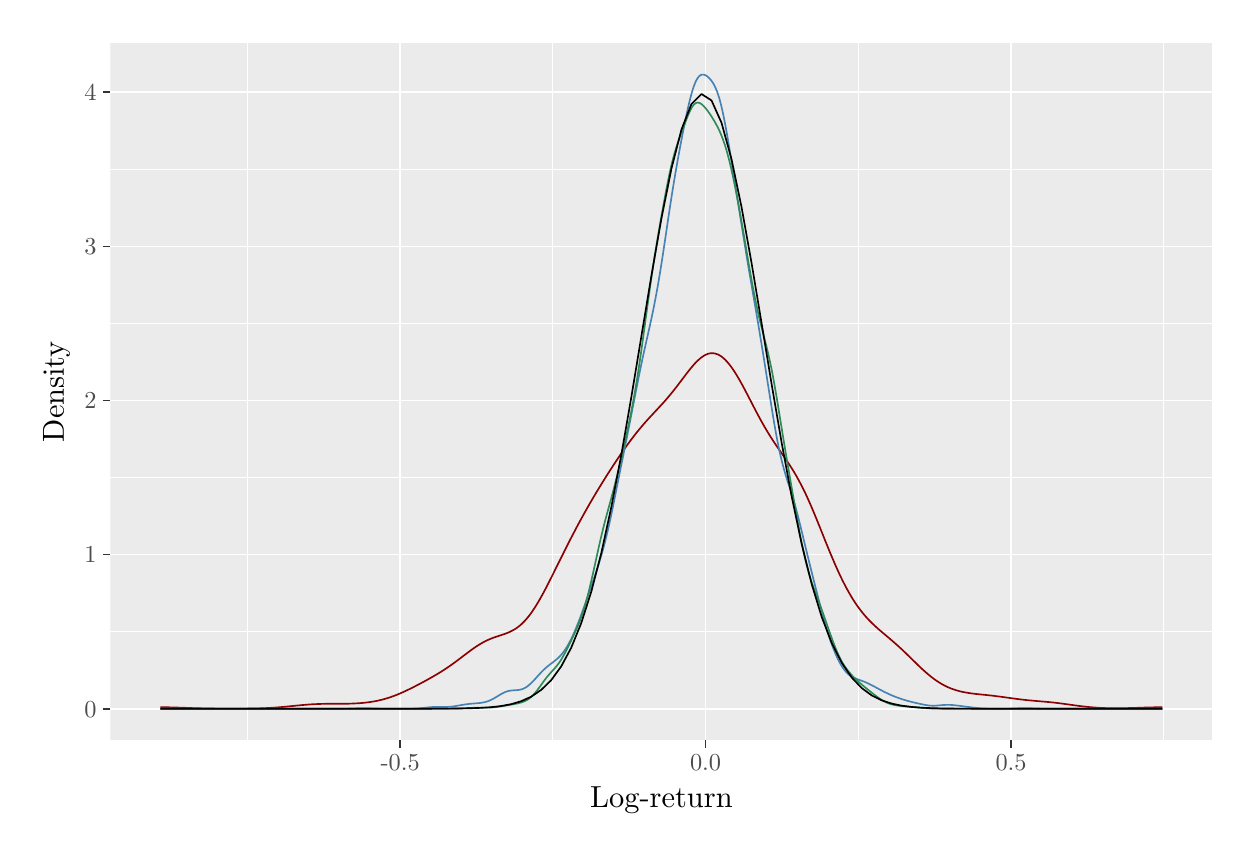
\begin{tikzpicture}[x=1pt,y=1pt]
\definecolor{fillColor}{RGB}{255,255,255}
\path[use as bounding box,fill=fillColor,fill opacity=0.00] (0,0) rectangle (433.62,289.08);
\begin{scope}
\path[clip] (  0.00,  0.00) rectangle (433.62,289.08);
\definecolor{drawColor}{RGB}{255,255,255}
\definecolor{fillColor}{RGB}{255,255,255}

\path[draw=drawColor,line width= 0.6pt,line join=round,line cap=round,fill=fillColor] (  0.00,  0.00) rectangle (433.62,289.08);
\end{scope}
\begin{scope}
\path[clip] ( 29.87, 31.53) rectangle (428.12,283.58);
\definecolor{fillColor}{gray}{0.92}

\path[fill=fillColor] ( 29.87, 31.53) rectangle (428.12,283.58);
\definecolor{drawColor}{RGB}{255,255,255}

\path[draw=drawColor,line width= 0.3pt,line join=round] ( 29.87, 70.83) --
	(428.12, 70.83);

\path[draw=drawColor,line width= 0.3pt,line join=round] ( 29.87,126.52) --
	(428.12,126.52);

\path[draw=drawColor,line width= 0.3pt,line join=round] ( 29.87,182.21) --
	(428.12,182.21);

\path[draw=drawColor,line width= 0.3pt,line join=round] ( 29.87,237.89) --
	(428.12,237.89);

\path[draw=drawColor,line width= 0.3pt,line join=round] ( 79.41, 31.53) --
	( 79.41,283.58);

\path[draw=drawColor,line width= 0.3pt,line join=round] (189.78, 31.53) --
	(189.78,283.58);

\path[draw=drawColor,line width= 0.3pt,line join=round] (300.16, 31.53) --
	(300.16,283.58);

\path[draw=drawColor,line width= 0.3pt,line join=round] (410.53, 31.53) --
	(410.53,283.58);

\path[draw=drawColor,line width= 0.6pt,line join=round] ( 29.87, 42.99) --
	(428.12, 42.99);

\path[draw=drawColor,line width= 0.6pt,line join=round] ( 29.87, 98.67) --
	(428.12, 98.67);

\path[draw=drawColor,line width= 0.6pt,line join=round] ( 29.87,154.36) --
	(428.12,154.36);

\path[draw=drawColor,line width= 0.6pt,line join=round] ( 29.87,210.05) --
	(428.12,210.05);

\path[draw=drawColor,line width= 0.6pt,line join=round] ( 29.87,265.74) --
	(428.12,265.74);

\path[draw=drawColor,line width= 0.6pt,line join=round] (134.60, 31.53) --
	(134.60,283.58);

\path[draw=drawColor,line width= 0.6pt,line join=round] (244.97, 31.53) --
	(244.97,283.58);

\path[draw=drawColor,line width= 0.6pt,line join=round] (355.35, 31.53) --
	(355.35,283.58);
\definecolor{drawColor}{RGB}{139,0,0}

\path[draw=drawColor,line width= 0.6pt,line join=round] ( 47.97, 43.52) --
	( 48.68, 43.52) --
	( 49.39, 43.51) --
	( 50.10, 43.50) --
	( 50.81, 43.49) --
	( 51.51, 43.48) --
	( 52.22, 43.46) --
	( 52.93, 43.44) --
	( 53.64, 43.42) --
	( 54.35, 43.40) --
	( 55.06, 43.37) --
	( 55.76, 43.35) --
	( 56.47, 43.32) --
	( 57.18, 43.30) --
	( 57.89, 43.27) --
	( 58.60, 43.25) --
	( 59.31, 43.22) --
	( 60.02, 43.20) --
	( 60.72, 43.18) --
	( 61.43, 43.16) --
	( 62.14, 43.14) --
	( 62.85, 43.12) --
	( 63.56, 43.10) --
	( 64.27, 43.09) --
	( 64.98, 43.07) --
	( 65.68, 43.06) --
	( 66.39, 43.05) --
	( 67.10, 43.04) --
	( 67.81, 43.03) --
	( 68.52, 43.02) --
	( 69.23, 43.02) --
	( 69.93, 43.01) --
	( 70.64, 43.01) --
	( 71.35, 43.01) --
	( 72.06, 43.00) --
	( 72.77, 43.00) --
	( 73.48, 43.00) --
	( 74.19, 43.00) --
	( 74.89, 43.00) --
	( 75.60, 43.00) --
	( 76.31, 43.01) --
	( 77.02, 43.01) --
	( 77.73, 43.01) --
	( 78.44, 43.02) --
	( 79.15, 43.03) --
	( 79.85, 43.04) --
	( 80.56, 43.05) --
	( 81.27, 43.06) --
	( 81.98, 43.07) --
	( 82.69, 43.09) --
	( 83.40, 43.11) --
	( 84.10, 43.13) --
	( 84.81, 43.15) --
	( 85.52, 43.18) --
	( 86.23, 43.21) --
	( 86.94, 43.25) --
	( 87.65, 43.29) --
	( 88.36, 43.33) --
	( 89.06, 43.37) --
	( 89.77, 43.42) --
	( 90.48, 43.48) --
	( 91.19, 43.54) --
	( 91.90, 43.60) --
	( 92.61, 43.66) --
	( 93.32, 43.73) --
	( 94.02, 43.80) --
	( 94.73, 43.87) --
	( 95.44, 43.94) --
	( 96.15, 44.01) --
	( 96.86, 44.08) --
	( 97.57, 44.15) --
	( 98.28, 44.22) --
	( 98.98, 44.29) --
	( 99.69, 44.35) --
	(100.40, 44.41) --
	(101.11, 44.47) --
	(101.82, 44.52) --
	(102.53, 44.57) --
	(103.23, 44.61) --
	(103.94, 44.64) --
	(104.65, 44.67) --
	(105.36, 44.70) --
	(106.07, 44.72) --
	(106.78, 44.74) --
	(107.49, 44.75) --
	(108.19, 44.75) --
	(108.90, 44.76) --
	(109.61, 44.76) --
	(110.32, 44.76) --
	(111.03, 44.76) --
	(111.74, 44.76) --
	(112.45, 44.76) --
	(113.15, 44.76) --
	(113.86, 44.77) --
	(114.57, 44.78) --
	(115.28, 44.79) --
	(115.99, 44.80) --
	(116.70, 44.82) --
	(117.40, 44.85) --
	(118.11, 44.88) --
	(118.82, 44.92) --
	(119.53, 44.96) --
	(120.24, 45.01) --
	(120.95, 45.07) --
	(121.66, 45.14) --
	(122.36, 45.22) --
	(123.07, 45.31) --
	(123.78, 45.41) --
	(124.49, 45.52) --
	(125.20, 45.64) --
	(125.91, 45.77) --
	(126.62, 45.92) --
	(127.32, 46.08) --
	(128.03, 46.25) --
	(128.74, 46.44) --
	(129.45, 46.64) --
	(130.16, 46.86) --
	(130.87, 47.09) --
	(131.57, 47.33) --
	(132.28, 47.59) --
	(132.99, 47.86) --
	(133.70, 48.14) --
	(134.41, 48.44) --
	(135.12, 48.75) --
	(135.83, 49.07) --
	(136.53, 49.39) --
	(137.24, 49.73) --
	(137.95, 50.07) --
	(138.66, 50.42) --
	(139.37, 50.78) --
	(140.08, 51.14) --
	(140.79, 51.51) --
	(141.49, 51.88) --
	(142.20, 52.25) --
	(142.91, 52.63) --
	(143.62, 53.02) --
	(144.33, 53.40) --
	(145.04, 53.80) --
	(145.74, 54.19) --
	(146.45, 54.60) --
	(147.16, 55.01) --
	(147.87, 55.43) --
	(148.58, 55.85) --
	(149.29, 56.29) --
	(150.00, 56.74) --
	(150.70, 57.20) --
	(151.41, 57.67) --
	(152.12, 58.15) --
	(152.83, 58.64) --
	(153.54, 59.14) --
	(154.25, 59.66) --
	(154.96, 60.18) --
	(155.66, 60.71) --
	(156.37, 61.25) --
	(157.08, 61.79) --
	(157.79, 62.33) --
	(158.50, 62.86) --
	(159.21, 63.40) --
	(159.92, 63.92) --
	(160.62, 64.44) --
	(161.33, 64.94) --
	(162.04, 65.42) --
	(162.75, 65.88) --
	(163.46, 66.32) --
	(164.17, 66.74) --
	(164.87, 67.12) --
	(165.58, 67.48) --
	(166.29, 67.82) --
	(167.00, 68.13) --
	(167.71, 68.42) --
	(168.42, 68.69) --
	(169.13, 68.93) --
	(169.83, 69.17) --
	(170.54, 69.40) --
	(171.25, 69.64) --
	(171.96, 69.87) --
	(172.67, 70.12) --
	(173.38, 70.39) --
	(174.09, 70.70) --
	(174.79, 71.03) --
	(175.50, 71.41) --
	(176.21, 71.83) --
	(176.92, 72.31) --
	(177.63, 72.85) --
	(178.34, 73.46) --
	(179.04, 74.13) --
	(179.75, 74.87) --
	(180.46, 75.68) --
	(181.17, 76.55) --
	(181.88, 77.50) --
	(182.59, 78.52) --
	(183.30, 79.60) --
	(184.00, 80.73) --
	(184.71, 81.92) --
	(185.42, 83.15) --
	(186.13, 84.44) --
	(186.84, 85.76) --
	(187.55, 87.12) --
	(188.26, 88.50) --
	(188.96, 89.90) --
	(189.67, 91.31) --
	(190.38, 92.74) --
	(191.09, 94.18) --
	(191.80, 95.61) --
	(192.51, 97.04) --
	(193.21, 98.47) --
	(193.92, 99.89) --
	(194.63,101.31) --
	(195.34,102.70) --
	(196.05,104.09) --
	(196.76,105.47) --
	(197.47,106.82) --
	(198.17,108.17) --
	(198.88,109.50) --
	(199.59,110.81) --
	(200.30,112.10) --
	(201.01,113.39) --
	(201.72,114.65) --
	(202.43,115.90) --
	(203.13,117.14) --
	(203.84,118.36) --
	(204.55,119.56) --
	(205.26,120.76) --
	(205.97,121.94) --
	(206.68,123.10) --
	(207.39,124.26) --
	(208.09,125.40) --
	(208.80,126.53) --
	(209.51,127.65) --
	(210.22,128.76) --
	(210.93,129.86) --
	(211.64,130.95) --
	(212.34,132.02) --
	(213.05,133.09) --
	(213.76,134.14) --
	(214.47,135.18) --
	(215.18,136.20) --
	(215.89,137.21) --
	(216.60,138.20) --
	(217.30,139.18) --
	(218.01,140.13) --
	(218.72,141.07) --
	(219.43,141.99) --
	(220.14,142.88) --
	(220.85,143.76) --
	(221.56,144.61) --
	(222.26,145.44) --
	(222.97,146.26) --
	(223.68,147.05) --
	(224.39,147.84) --
	(225.10,148.61) --
	(225.81,149.37) --
	(226.51,150.13) --
	(227.22,150.88) --
	(227.93,151.64) --
	(228.64,152.41) --
	(229.35,153.18) --
	(230.06,153.97) --
	(230.77,154.78) --
	(231.47,155.60) --
	(232.18,156.45) --
	(232.89,157.31) --
	(233.60,158.20) --
	(234.31,159.10) --
	(235.02,160.02) --
	(235.73,160.96) --
	(236.43,161.89) --
	(237.14,162.83) --
	(237.85,163.77) --
	(238.56,164.69) --
	(239.27,165.58) --
	(239.98,166.44) --
	(240.68,167.27) --
	(241.39,168.05) --
	(242.10,168.76) --
	(242.81,169.40) --
	(243.52,169.97) --
	(244.23,170.45) --
	(244.94,170.85) --
	(245.64,171.16) --
	(246.35,171.37) --
	(247.06,171.45) --
	(247.77,171.43) --
	(248.48,171.31) --
	(249.19,171.08) --
	(249.90,170.75) --
	(250.60,170.32) --
	(251.31,169.76) --
	(252.02,169.11) --
	(252.73,168.36) --
	(253.44,167.52) --
	(254.15,166.61) --
	(254.85,165.61) --
	(255.56,164.53) --
	(256.27,163.39) --
	(256.98,162.19) --
	(257.69,160.94) --
	(258.40,159.65) --
	(259.11,158.33) --
	(259.81,156.98) --
	(260.52,155.61) --
	(261.23,154.24) --
	(261.94,152.87) --
	(262.65,151.50) --
	(263.36,150.14) --
	(264.07,148.81) --
	(264.77,147.50) --
	(265.48,146.23) --
	(266.19,144.98) --
	(266.90,143.77) --
	(267.61,142.59) --
	(268.32,141.45) --
	(269.03,140.34) --
	(269.73,139.26) --
	(270.44,138.20) --
	(271.15,137.16) --
	(271.86,136.14) --
	(272.57,135.12) --
	(273.28,134.10) --
	(273.98,133.07) --
	(274.69,132.02) --
	(275.40,130.94) --
	(276.11,129.84) --
	(276.82,128.69) --
	(277.53,127.49) --
	(278.24,126.24) --
	(278.94,124.94) --
	(279.65,123.58) --
	(280.36,122.17) --
	(281.07,120.70) --
	(281.78,119.17) --
	(282.49,117.58) --
	(283.20,115.96) --
	(283.90,114.29) --
	(284.61,112.59) --
	(285.32,110.85) --
	(286.03,109.10) --
	(286.74,107.33) --
	(287.45,105.56) --
	(288.15,103.79) --
	(288.86,102.04) --
	(289.57,100.30) --
	(290.28, 98.59) --
	(290.99, 96.91) --
	(291.70, 95.27) --
	(292.41, 93.66) --
	(293.11, 92.11) --
	(293.82, 90.60) --
	(294.53, 89.15) --
	(295.24, 87.76) --
	(295.95, 86.42) --
	(296.66, 85.14) --
	(297.37, 83.91) --
	(298.07, 82.74) --
	(298.78, 81.63) --
	(299.49, 80.58) --
	(300.20, 79.58) --
	(300.91, 78.63) --
	(301.62, 77.72) --
	(302.32, 76.87) --
	(303.03, 76.06) --
	(303.74, 75.29) --
	(304.45, 74.55) --
	(305.16, 73.85) --
	(305.87, 73.17) --
	(306.58, 72.52) --
	(307.28, 71.88) --
	(307.99, 71.27) --
	(308.70, 70.66) --
	(309.41, 70.06) --
	(310.12, 69.47) --
	(310.83, 68.87) --
	(311.54, 68.27) --
	(312.24, 67.67) --
	(312.95, 67.05) --
	(313.66, 66.43) --
	(314.37, 65.80) --
	(315.08, 65.15) --
	(315.79, 64.50) --
	(316.49, 63.83) --
	(317.20, 63.15) --
	(317.91, 62.46) --
	(318.62, 61.77) --
	(319.33, 61.08) --
	(320.04, 60.38) --
	(320.75, 59.69) --
	(321.45, 59.00) --
	(322.16, 58.32) --
	(322.87, 57.65) --
	(323.58, 57.00) --
	(324.29, 56.36) --
	(325.00, 55.74) --
	(325.71, 55.15) --
	(326.41, 54.57) --
	(327.12, 54.02) --
	(327.83, 53.50) --
	(328.54, 53.01) --
	(329.25, 52.54) --
	(329.96, 52.11) --
	(330.67, 51.70) --
	(331.37, 51.33) --
	(332.08, 50.98) --
	(332.79, 50.65) --
	(333.50, 50.36) --
	(334.21, 50.09) --
	(334.92, 49.85) --
	(335.62, 49.63) --
	(336.33, 49.42) --
	(337.04, 49.24) --
	(337.75, 49.08) --
	(338.46, 48.94) --
	(339.17, 48.81) --
	(339.88, 48.69) --
	(340.58, 48.58) --
	(341.29, 48.48) --
	(342.00, 48.40) --
	(342.71, 48.31) --
	(343.42, 48.24) --
	(344.13, 48.16) --
	(344.84, 48.09) --
	(345.54, 48.02) --
	(346.25, 47.95) --
	(346.96, 47.87) --
	(347.67, 47.80) --
	(348.38, 47.72) --
	(349.09, 47.64) --
	(349.79, 47.55) --
	(350.50, 47.46) --
	(351.21, 47.37) --
	(351.92, 47.28) --
	(352.63, 47.18) --
	(353.34, 47.08) --
	(354.05, 46.98) --
	(354.75, 46.88) --
	(355.46, 46.78) --
	(356.17, 46.69) --
	(356.88, 46.59) --
	(357.59, 46.50) --
	(358.30, 46.41) --
	(359.01, 46.32) --
	(359.71, 46.24) --
	(360.42, 46.16) --
	(361.13, 46.09) --
	(361.84, 46.02) --
	(362.55, 45.95) --
	(363.26, 45.89) --
	(363.96, 45.82) --
	(364.67, 45.76) --
	(365.38, 45.70) --
	(366.09, 45.64) --
	(366.80, 45.58) --
	(367.51, 45.52) --
	(368.22, 45.46) --
	(368.92, 45.39) --
	(369.63, 45.32) --
	(370.34, 45.25) --
	(371.05, 45.17) --
	(371.76, 45.09) --
	(372.47, 45.00) --
	(373.18, 44.91) --
	(373.88, 44.82) --
	(374.59, 44.72) --
	(375.30, 44.63) --
	(376.01, 44.53) --
	(376.72, 44.43) --
	(377.43, 44.33) --
	(378.13, 44.23) --
	(378.84, 44.14) --
	(379.55, 44.04) --
	(380.26, 43.95) --
	(380.97, 43.86) --
	(381.68, 43.78) --
	(382.39, 43.70) --
	(383.09, 43.63) --
	(383.80, 43.56) --
	(384.51, 43.50) --
	(385.22, 43.44) --
	(385.93, 43.39) --
	(386.64, 43.34) --
	(387.35, 43.30) --
	(388.05, 43.26) --
	(388.76, 43.23) --
	(389.47, 43.21) --
	(390.18, 43.19) --
	(390.89, 43.17) --
	(391.60, 43.16) --
	(392.31, 43.15) --
	(393.01, 43.15) --
	(393.72, 43.15) --
	(394.43, 43.15) --
	(395.14, 43.16) --
	(395.85, 43.17) --
	(396.56, 43.18) --
	(397.26, 43.20) --
	(397.97, 43.22) --
	(398.68, 43.24) --
	(399.39, 43.26) --
	(400.10, 43.28) --
	(400.81, 43.30) --
	(401.52, 43.33) --
	(402.22, 43.35) --
	(402.93, 43.38) --
	(403.64, 43.40) --
	(404.35, 43.42) --
	(405.06, 43.44) --
	(405.77, 43.46) --
	(406.48, 43.48) --
	(407.18, 43.49) --
	(407.89, 43.50) --
	(408.60, 43.51) --
	(409.31, 43.52) --
	(410.02, 43.52);
\definecolor{drawColor}{RGB}{70,130,180}

\path[draw=drawColor,line width= 0.6pt,line join=round] ( 47.97, 42.99) --
	( 48.68, 42.99) --
	( 49.39, 42.99) --
	( 50.10, 42.99) --
	( 50.81, 42.99) --
	( 51.51, 42.99) --
	( 52.22, 42.99) --
	( 52.93, 42.99) --
	( 53.64, 42.99) --
	( 54.35, 42.99) --
	( 55.06, 42.99) --
	( 55.76, 42.99) --
	( 56.47, 42.99) --
	( 57.18, 42.99) --
	( 57.89, 42.99) --
	( 58.60, 42.99) --
	( 59.31, 42.99) --
	( 60.02, 42.99) --
	( 60.72, 42.99) --
	( 61.43, 42.99) --
	( 62.14, 42.99) --
	( 62.85, 42.99) --
	( 63.56, 42.99) --
	( 64.27, 42.99) --
	( 64.98, 42.99) --
	( 65.68, 42.99) --
	( 66.39, 42.99) --
	( 67.10, 42.99) --
	( 67.81, 42.99) --
	( 68.52, 42.99) --
	( 69.23, 42.99) --
	( 69.93, 42.99) --
	( 70.64, 42.99) --
	( 71.35, 42.99) --
	( 72.06, 42.99) --
	( 72.77, 42.99) --
	( 73.48, 42.99) --
	( 74.19, 42.99) --
	( 74.89, 42.99) --
	( 75.60, 42.99) --
	( 76.31, 42.99) --
	( 77.02, 42.99) --
	( 77.73, 42.99) --
	( 78.44, 42.99) --
	( 79.15, 42.99) --
	( 79.85, 42.99) --
	( 80.56, 42.99) --
	( 81.27, 42.99) --
	( 81.98, 42.99) --
	( 82.69, 42.99) --
	( 83.40, 42.99) --
	( 84.10, 42.99) --
	( 84.81, 42.99) --
	( 85.52, 42.99) --
	( 86.23, 42.99) --
	( 86.94, 42.99) --
	( 87.65, 42.99) --
	( 88.36, 42.99) --
	( 89.06, 42.99) --
	( 89.77, 42.99) --
	( 90.48, 42.99) --
	( 91.19, 42.99) --
	( 91.90, 42.99) --
	( 92.61, 42.99) --
	( 93.32, 42.99) --
	( 94.02, 42.99) --
	( 94.73, 42.99) --
	( 95.44, 42.99) --
	( 96.15, 42.99) --
	( 96.86, 42.99) --
	( 97.57, 42.99) --
	( 98.28, 42.99) --
	( 98.98, 42.99) --
	( 99.69, 42.99) --
	(100.40, 42.99) --
	(101.11, 42.99) --
	(101.82, 42.99) --
	(102.53, 42.99) --
	(103.23, 42.99) --
	(103.94, 42.99) --
	(104.65, 42.99) --
	(105.36, 42.99) --
	(106.07, 42.99) --
	(106.78, 42.99) --
	(107.49, 42.99) --
	(108.19, 42.99) --
	(108.90, 42.99) --
	(109.61, 42.99) --
	(110.32, 42.99) --
	(111.03, 42.99) --
	(111.74, 42.99) --
	(112.45, 42.99) --
	(113.15, 43.00) --
	(113.86, 43.00) --
	(114.57, 43.01) --
	(115.28, 43.02) --
	(115.99, 43.04) --
	(116.70, 43.06) --
	(117.40, 43.08) --
	(118.11, 43.10) --
	(118.82, 43.13) --
	(119.53, 43.15) --
	(120.24, 43.17) --
	(120.95, 43.17) --
	(121.66, 43.18) --
	(122.36, 43.17) --
	(123.07, 43.15) --
	(123.78, 43.13) --
	(124.49, 43.11) --
	(125.20, 43.08) --
	(125.91, 43.06) --
	(126.62, 43.04) --
	(127.32, 43.02) --
	(128.03, 43.01) --
	(128.74, 43.00) --
	(129.45, 43.00) --
	(130.16, 42.99) --
	(130.87, 42.99) --
	(131.57, 42.99) --
	(132.28, 42.99) --
	(132.99, 42.99) --
	(133.70, 42.99) --
	(134.41, 42.99) --
	(135.12, 42.99) --
	(135.83, 42.99) --
	(136.53, 42.99) --
	(137.24, 43.00) --
	(137.95, 43.00) --
	(138.66, 43.01) --
	(139.37, 43.03) --
	(140.08, 43.06) --
	(140.79, 43.09) --
	(141.49, 43.14) --
	(142.20, 43.20) --
	(142.91, 43.27) --
	(143.62, 43.34) --
	(144.33, 43.42) --
	(145.04, 43.49) --
	(145.74, 43.55) --
	(146.45, 43.60) --
	(147.16, 43.62) --
	(147.87, 43.63) --
	(148.58, 43.62) --
	(149.29, 43.61) --
	(150.00, 43.60) --
	(150.70, 43.60) --
	(151.41, 43.61) --
	(152.12, 43.65) --
	(152.83, 43.70) --
	(153.54, 43.78) --
	(154.25, 43.88) --
	(154.96, 44.00) --
	(155.66, 44.12) --
	(156.37, 44.25) --
	(157.08, 44.37) --
	(157.79, 44.49) --
	(158.50, 44.59) --
	(159.21, 44.68) --
	(159.92, 44.76) --
	(160.62, 44.82) --
	(161.33, 44.88) --
	(162.04, 44.93) --
	(162.75, 44.99) --
	(163.46, 45.06) --
	(164.17, 45.16) --
	(164.87, 45.30) --
	(165.58, 45.47) --
	(166.29, 45.70) --
	(167.00, 45.98) --
	(167.71, 46.32) --
	(168.42, 46.69) --
	(169.13, 47.10) --
	(169.83, 47.53) --
	(170.54, 47.96) --
	(171.25, 48.37) --
	(171.96, 48.74) --
	(172.67, 49.05) --
	(173.38, 49.29) --
	(174.09, 49.46) --
	(174.79, 49.57) --
	(175.50, 49.63) --
	(176.21, 49.67) --
	(176.92, 49.71) --
	(177.63, 49.79) --
	(178.34, 49.95) --
	(179.04, 50.19) --
	(179.75, 50.53) --
	(180.46, 50.99) --
	(181.17, 51.54) --
	(181.88, 52.18) --
	(182.59, 52.89) --
	(183.30, 53.65) --
	(184.00, 54.43) --
	(184.71, 55.21) --
	(185.42, 55.98) --
	(186.13, 56.71) --
	(186.84, 57.39) --
	(187.55, 58.02) --
	(188.26, 58.60) --
	(188.96, 59.15) --
	(189.67, 59.68) --
	(190.38, 60.23) --
	(191.09, 60.80) --
	(191.80, 61.43) --
	(192.51, 62.15) --
	(193.21, 62.97) --
	(193.92, 63.90) --
	(194.63, 64.96) --
	(195.34, 66.16) --
	(196.05, 67.48) --
	(196.76, 68.91) --
	(197.47, 70.47) --
	(198.17, 72.13) --
	(198.88, 73.89) --
	(199.59, 75.74) --
	(200.30, 77.66) --
	(201.01, 79.63) --
	(201.72, 81.64) --
	(202.43, 83.68) --
	(203.13, 85.72) --
	(203.84, 87.77) --
	(204.55, 89.84) --
	(205.26, 91.94) --
	(205.97, 94.10) --
	(206.68, 96.35) --
	(207.39, 98.72) --
	(208.09,101.25) --
	(208.80,103.97) --
	(209.51,106.90) --
	(210.22,110.01) --
	(210.93,113.30) --
	(211.64,116.73) --
	(212.34,120.24) --
	(213.05,123.80) --
	(213.76,127.36) --
	(214.47,130.89) --
	(215.18,134.40) --
	(215.89,137.90) --
	(216.60,141.42) --
	(217.30,144.98) --
	(218.01,148.59) --
	(218.72,152.25) --
	(219.43,155.92) --
	(220.14,159.56) --
	(220.85,163.12) --
	(221.56,166.57) --
	(222.26,169.91) --
	(222.97,173.14) --
	(223.68,176.30) --
	(224.39,179.44) --
	(225.10,182.63) --
	(225.81,185.94) --
	(226.51,189.44) --
	(227.22,193.16) --
	(227.93,197.16) --
	(228.64,201.43) --
	(229.35,205.94) --
	(230.06,210.64) --
	(230.77,215.42) --
	(231.47,220.19) --
	(232.18,224.88) --
	(232.89,229.43) --
	(233.60,233.80) --
	(234.31,237.97) --
	(235.02,241.98) --
	(235.73,245.83) --
	(236.43,249.55) --
	(237.14,253.15) --
	(237.85,256.62) --
	(238.56,259.90) --
	(239.27,262.93) --
	(239.98,265.61) --
	(240.68,267.85) --
	(241.39,269.62) --
	(242.10,270.90) --
	(242.81,271.71) --
	(243.52,272.09) --
	(244.23,272.12) --
	(244.94,271.88) --
	(245.64,271.42) --
	(246.35,270.77) --
	(247.06,269.94) --
	(247.77,268.88) --
	(248.48,267.53) --
	(249.19,265.81) --
	(249.90,263.66) --
	(250.60,260.99) --
	(251.31,257.86) --
	(252.02,254.30) --
	(252.73,250.39) --
	(253.44,246.23) --
	(254.15,241.90) --
	(254.85,237.48) --
	(255.56,233.00) --
	(256.27,228.50) --
	(256.98,224.01) --
	(257.69,219.54) --
	(258.40,215.10) --
	(259.11,210.72) --
	(259.81,206.40) --
	(260.52,202.17) --
	(261.23,198.01) --
	(261.94,193.89) --
	(262.65,189.78) --
	(263.36,185.65) --
	(264.07,181.47) --
	(264.77,177.22) --
	(265.48,172.89) --
	(266.19,168.48) --
	(266.90,164.00) --
	(267.61,159.49) --
	(268.32,155.00) --
	(269.03,150.57) --
	(269.73,146.30) --
	(270.44,142.25) --
	(271.15,138.52) --
	(271.86,135.17) --
	(272.57,132.18) --
	(273.28,129.52) --
	(273.98,127.12) --
	(274.69,124.88) --
	(275.40,122.70) --
	(276.11,120.47) --
	(276.82,118.12) --
	(277.53,115.62) --
	(278.24,112.96) --
	(278.94,110.17) --
	(279.65,107.27) --
	(280.36,104.33) --
	(281.07,101.39) --
	(281.78, 98.47) --
	(282.49, 95.59) --
	(283.20, 92.75) --
	(283.90, 89.94) --
	(284.61, 87.14) --
	(285.32, 84.36) --
	(286.03, 81.62) --
	(286.74, 78.92) --
	(287.45, 76.30) --
	(288.15, 73.78) --
	(288.86, 71.38) --
	(289.57, 69.13) --
	(290.28, 67.03) --
	(290.99, 65.09) --
	(291.70, 63.31) --
	(292.41, 61.69) --
	(293.11, 60.23) --
	(293.82, 58.93) --
	(294.53, 57.79) --
	(295.24, 56.82) --
	(295.95, 56.01) --
	(296.66, 55.34) --
	(297.37, 54.81) --
	(298.07, 54.38) --
	(298.78, 54.04) --
	(299.49, 53.75) --
	(300.20, 53.50) --
	(300.91, 53.25) --
	(301.62, 52.99) --
	(302.32, 52.72) --
	(303.03, 52.42) --
	(303.74, 52.09) --
	(304.45, 51.75) --
	(305.16, 51.39) --
	(305.87, 51.02) --
	(306.58, 50.64) --
	(307.28, 50.26) --
	(307.99, 49.88) --
	(308.70, 49.51) --
	(309.41, 49.14) --
	(310.12, 48.79) --
	(310.83, 48.45) --
	(311.54, 48.12) --
	(312.24, 47.81) --
	(312.95, 47.52) --
	(313.66, 47.24) --
	(314.37, 46.98) --
	(315.08, 46.73) --
	(315.79, 46.49) --
	(316.49, 46.26) --
	(317.20, 46.05) --
	(317.91, 45.84) --
	(318.62, 45.64) --
	(319.33, 45.46) --
	(320.04, 45.29) --
	(320.75, 45.12) --
	(321.45, 44.96) --
	(322.16, 44.80) --
	(322.87, 44.65) --
	(323.58, 44.50) --
	(324.29, 44.36) --
	(325.00, 44.24) --
	(325.71, 44.15) --
	(326.41, 44.09) --
	(327.12, 44.07) --
	(327.83, 44.08) --
	(328.54, 44.12) --
	(329.25, 44.18) --
	(329.96, 44.25) --
	(330.67, 44.31) --
	(331.37, 44.35) --
	(332.08, 44.38) --
	(332.79, 44.38) --
	(333.50, 44.36) --
	(334.21, 44.31) --
	(334.92, 44.24) --
	(335.62, 44.16) --
	(336.33, 44.08) --
	(337.04, 43.99) --
	(337.75, 43.90) --
	(338.46, 43.80) --
	(339.17, 43.71) --
	(339.88, 43.62) --
	(340.58, 43.53) --
	(341.29, 43.44) --
	(342.00, 43.36) --
	(342.71, 43.28) --
	(343.42, 43.21) --
	(344.13, 43.15) --
	(344.84, 43.10) --
	(345.54, 43.07) --
	(346.25, 43.04) --
	(346.96, 43.02) --
	(347.67, 43.01) --
	(348.38, 43.00) --
	(349.09, 42.99) --
	(349.79, 42.99) --
	(350.50, 42.99) --
	(351.21, 42.99) --
	(351.92, 43.00) --
	(352.63, 43.00) --
	(353.34, 43.01) --
	(354.05, 43.02) --
	(354.75, 43.03) --
	(355.46, 43.05) --
	(356.17, 43.07) --
	(356.88, 43.10) --
	(357.59, 43.12) --
	(358.30, 43.14) --
	(359.01, 43.16) --
	(359.71, 43.17) --
	(360.42, 43.18) --
	(361.13, 43.17) --
	(361.84, 43.16) --
	(362.55, 43.14) --
	(363.26, 43.12) --
	(363.96, 43.09) --
	(364.67, 43.07) --
	(365.38, 43.05) --
	(366.09, 43.03) --
	(366.80, 43.02) --
	(367.51, 43.01) --
	(368.22, 43.00) --
	(368.92, 42.99) --
	(369.63, 42.99) --
	(370.34, 42.99) --
	(371.05, 42.99) --
	(371.76, 42.99) --
	(372.47, 42.99) --
	(373.18, 42.99) --
	(373.88, 42.99) --
	(374.59, 42.99) --
	(375.30, 42.99) --
	(376.01, 42.99) --
	(376.72, 42.99) --
	(377.43, 42.99) --
	(378.13, 42.99) --
	(378.84, 42.99) --
	(379.55, 42.99) --
	(380.26, 42.99) --
	(380.97, 42.99) --
	(381.68, 42.99) --
	(382.39, 42.99) --
	(383.09, 42.99) --
	(383.80, 42.99) --
	(384.51, 42.99) --
	(385.22, 42.99) --
	(385.93, 42.99) --
	(386.64, 42.99) --
	(387.35, 42.99) --
	(388.05, 42.99) --
	(388.76, 42.99) --
	(389.47, 42.99) --
	(390.18, 42.99) --
	(390.89, 42.99) --
	(391.60, 42.99) --
	(392.31, 42.99) --
	(393.01, 42.99) --
	(393.72, 42.99) --
	(394.43, 42.99) --
	(395.14, 42.99) --
	(395.85, 42.99) --
	(396.56, 42.99) --
	(397.26, 42.99) --
	(397.97, 42.99) --
	(398.68, 42.99) --
	(399.39, 42.99) --
	(400.10, 42.99) --
	(400.81, 42.99) --
	(401.52, 42.99) --
	(402.22, 42.99) --
	(402.93, 42.99) --
	(403.64, 42.99) --
	(404.35, 42.99) --
	(405.06, 42.99) --
	(405.77, 42.99) --
	(406.48, 42.99) --
	(407.18, 42.99) --
	(407.89, 42.99) --
	(408.60, 42.99) --
	(409.31, 42.99) --
	(410.02, 42.99);
\definecolor{drawColor}{RGB}{46,139,87}

\path[draw=drawColor,line width= 0.6pt,line join=round] ( 47.97, 42.99) --
	( 48.68, 42.99) --
	( 49.39, 42.99) --
	( 50.10, 42.99) --
	( 50.81, 42.99) --
	( 51.51, 42.99) --
	( 52.22, 42.99) --
	( 52.93, 42.99) --
	( 53.64, 42.99) --
	( 54.35, 42.99) --
	( 55.06, 42.99) --
	( 55.76, 42.99) --
	( 56.47, 42.99) --
	( 57.18, 42.99) --
	( 57.89, 42.99) --
	( 58.60, 42.99) --
	( 59.31, 42.99) --
	( 60.02, 42.99) --
	( 60.72, 42.99) --
	( 61.43, 42.99) --
	( 62.14, 42.99) --
	( 62.85, 42.99) --
	( 63.56, 42.99) --
	( 64.27, 42.99) --
	( 64.98, 42.99) --
	( 65.68, 42.99) --
	( 66.39, 42.99) --
	( 67.10, 42.99) --
	( 67.81, 42.99) --
	( 68.52, 42.99) --
	( 69.23, 42.99) --
	( 69.93, 42.99) --
	( 70.64, 42.99) --
	( 71.35, 42.99) --
	( 72.06, 42.99) --
	( 72.77, 42.99) --
	( 73.48, 42.99) --
	( 74.19, 42.99) --
	( 74.89, 42.99) --
	( 75.60, 42.99) --
	( 76.31, 42.99) --
	( 77.02, 42.99) --
	( 77.73, 42.99) --
	( 78.44, 42.99) --
	( 79.15, 42.99) --
	( 79.85, 42.99) --
	( 80.56, 42.99) --
	( 81.27, 42.99) --
	( 81.98, 42.99) --
	( 82.69, 42.99) --
	( 83.40, 42.99) --
	( 84.10, 42.99) --
	( 84.81, 42.99) --
	( 85.52, 42.99) --
	( 86.23, 42.99) --
	( 86.94, 42.99) --
	( 87.65, 42.99) --
	( 88.36, 42.99) --
	( 89.06, 42.99) --
	( 89.77, 42.99) --
	( 90.48, 42.99) --
	( 91.19, 42.99) --
	( 91.90, 42.99) --
	( 92.61, 42.99) --
	( 93.32, 42.99) --
	( 94.02, 42.99) --
	( 94.73, 42.99) --
	( 95.44, 42.99) --
	( 96.15, 42.99) --
	( 96.86, 42.99) --
	( 97.57, 42.99) --
	( 98.28, 42.99) --
	( 98.98, 42.99) --
	( 99.69, 42.99) --
	(100.40, 42.99) --
	(101.11, 42.99) --
	(101.82, 42.99) --
	(102.53, 42.99) --
	(103.23, 42.99) --
	(103.94, 42.99) --
	(104.65, 42.99) --
	(105.36, 42.99) --
	(106.07, 42.99) --
	(106.78, 42.99) --
	(107.49, 42.99) --
	(108.19, 42.99) --
	(108.90, 42.99) --
	(109.61, 42.99) --
	(110.32, 42.99) --
	(111.03, 42.99) --
	(111.74, 42.99) --
	(112.45, 42.99) --
	(113.15, 42.99) --
	(113.86, 42.99) --
	(114.57, 42.99) --
	(115.28, 42.99) --
	(115.99, 42.99) --
	(116.70, 42.99) --
	(117.40, 42.99) --
	(118.11, 42.99) --
	(118.82, 42.99) --
	(119.53, 42.99) --
	(120.24, 42.99) --
	(120.95, 42.99) --
	(121.66, 42.99) --
	(122.36, 42.99) --
	(123.07, 42.99) --
	(123.78, 42.99) --
	(124.49, 42.99) --
	(125.20, 42.99) --
	(125.91, 42.99) --
	(126.62, 42.99) --
	(127.32, 42.99) --
	(128.03, 42.99) --
	(128.74, 42.99) --
	(129.45, 42.99) --
	(130.16, 42.99) --
	(130.87, 42.99) --
	(131.57, 42.99) --
	(132.28, 42.99) --
	(132.99, 42.99) --
	(133.70, 42.99) --
	(134.41, 42.99) --
	(135.12, 42.99) --
	(135.83, 42.99) --
	(136.53, 42.99) --
	(137.24, 42.99) --
	(137.95, 42.99) --
	(138.66, 42.99) --
	(139.37, 42.99) --
	(140.08, 42.99) --
	(140.79, 42.99) --
	(141.49, 42.99) --
	(142.20, 42.99) --
	(142.91, 42.99) --
	(143.62, 42.99) --
	(144.33, 42.99) --
	(145.04, 42.99) --
	(145.74, 42.99) --
	(146.45, 42.99) --
	(147.16, 42.99) --
	(147.87, 42.99) --
	(148.58, 42.99) --
	(149.29, 42.99) --
	(150.00, 42.99) --
	(150.70, 42.99) --
	(151.41, 43.00) --
	(152.12, 43.00) --
	(152.83, 43.01) --
	(153.54, 43.03) --
	(154.25, 43.04) --
	(154.96, 43.06) --
	(155.66, 43.09) --
	(156.37, 43.12) --
	(157.08, 43.15) --
	(157.79, 43.18) --
	(158.50, 43.21) --
	(159.21, 43.24) --
	(159.92, 43.27) --
	(160.62, 43.30) --
	(161.33, 43.32) --
	(162.04, 43.34) --
	(162.75, 43.36) --
	(163.46, 43.37) --
	(164.17, 43.37) --
	(164.87, 43.37) --
	(165.58, 43.37) --
	(166.29, 43.38) --
	(167.00, 43.40) --
	(167.71, 43.43) --
	(168.42, 43.49) --
	(169.13, 43.56) --
	(169.83, 43.65) --
	(170.54, 43.76) --
	(171.25, 43.87) --
	(171.96, 43.99) --
	(172.67, 44.12) --
	(173.38, 44.24) --
	(174.09, 44.37) --
	(174.79, 44.49) --
	(175.50, 44.61) --
	(176.21, 44.74) --
	(176.92, 44.88) --
	(177.63, 45.04) --
	(178.34, 45.24) --
	(179.04, 45.48) --
	(179.75, 45.77) --
	(180.46, 46.15) --
	(181.17, 46.61) --
	(181.88, 47.17) --
	(182.59, 47.85) --
	(183.30, 48.62) --
	(184.00, 49.49) --
	(184.71, 50.44) --
	(185.42, 51.42) --
	(186.13, 52.42) --
	(186.84, 53.39) --
	(187.55, 54.31) --
	(188.26, 55.16) --
	(188.96, 55.96) --
	(189.67, 56.74) --
	(190.38, 57.52) --
	(191.09, 58.35) --
	(191.80, 59.26) --
	(192.51, 60.29) --
	(193.21, 61.43) --
	(193.92, 62.69) --
	(194.63, 64.03) --
	(195.34, 65.45) --
	(196.05, 66.90) --
	(196.76, 68.38) --
	(197.47, 69.89) --
	(198.17, 71.45) --
	(198.88, 73.10) --
	(199.59, 74.88) --
	(200.30, 76.84) --
	(201.01, 79.01) --
	(201.72, 81.42) --
	(202.43, 84.06) --
	(203.13, 86.92) --
	(203.84, 89.96) --
	(204.55, 93.13) --
	(205.26, 96.36) --
	(205.97, 99.60) --
	(206.68,102.76) --
	(207.39,105.81) --
	(208.09,108.69) --
	(208.80,111.44) --
	(209.51,114.07) --
	(210.22,116.65) --
	(210.93,119.23) --
	(211.64,121.86) --
	(212.34,124.58) --
	(213.05,127.42) --
	(213.76,130.36) --
	(214.47,133.40) --
	(215.18,136.52) --
	(215.89,139.71) --
	(216.60,142.98) --
	(217.30,146.35) --
	(218.01,149.86) --
	(218.72,153.57) --
	(219.43,157.53) --
	(220.14,161.77) --
	(220.85,166.31) --
	(221.56,171.12) --
	(222.26,176.15) --
	(222.97,181.33) --
	(223.68,186.56) --
	(224.39,191.73) --
	(225.10,196.75) --
	(225.81,201.57) --
	(226.51,206.17) --
	(227.22,210.56) --
	(227.93,214.78) --
	(228.64,218.87) --
	(229.35,222.87) --
	(230.06,226.77) --
	(230.77,230.55) --
	(231.47,234.14) --
	(232.18,237.48) --
	(232.89,240.50) --
	(233.60,243.20) --
	(234.31,245.60) --
	(235.02,247.75) --
	(235.73,249.75) --
	(236.43,251.67) --
	(237.14,253.56) --
	(237.85,255.44) --
	(238.56,257.25) --
	(239.27,258.89) --
	(239.98,260.26) --
	(240.68,261.25) --
	(241.39,261.83) --
	(242.10,262.02) --
	(242.81,261.87) --
	(243.52,261.43) --
	(244.23,260.79) --
	(244.94,260.00) --
	(245.64,259.10) --
	(246.35,258.12) --
	(247.06,257.06) --
	(247.77,255.93) --
	(248.48,254.71) --
	(249.19,253.40) --
	(249.90,251.96) --
	(250.60,250.35) --
	(251.31,248.52) --
	(252.02,246.42) --
	(252.73,244.05) --
	(253.44,241.39) --
	(254.15,238.45) --
	(254.85,235.27) --
	(255.56,231.86) --
	(256.27,228.24) --
	(256.98,224.45) --
	(257.69,220.50) --
	(258.40,216.43) --
	(259.11,212.26) --
	(259.81,208.06) --
	(260.52,203.88) --
	(261.23,199.79) --
	(261.94,195.86) --
	(262.65,192.15) --
	(263.36,188.69) --
	(264.07,185.47) --
	(264.77,182.48) --
	(265.48,179.65) --
	(266.19,176.89) --
	(266.90,174.10) --
	(267.61,171.17) --
	(268.32,168.00) --
	(269.03,164.52) --
	(269.73,160.73) --
	(270.44,156.66) --
	(271.15,152.39) --
	(271.86,148.01) --
	(272.57,143.61) --
	(273.28,139.28) --
	(273.98,135.03) --
	(274.69,130.85) --
	(275.40,126.73) --
	(276.11,122.63) --
	(276.82,118.55) --
	(277.53,114.49) --
	(278.24,110.51) --
	(278.94,106.66) --
	(279.65,103.01) --
	(280.36, 99.62) --
	(281.07, 96.52) --
	(281.78, 93.73) --
	(282.49, 91.23) --
	(283.20, 88.98) --
	(283.90, 86.92) --
	(284.61, 84.97) --
	(285.32, 83.08) --
	(286.03, 81.20) --
	(286.74, 79.29) --
	(287.45, 77.33) --
	(288.15, 75.33) --
	(288.86, 73.29) --
	(289.57, 71.25) --
	(290.28, 69.24) --
	(290.99, 67.29) --
	(291.70, 65.44) --
	(292.41, 63.72) --
	(293.11, 62.13) --
	(293.82, 60.71) --
	(294.53, 59.44) --
	(295.24, 58.31) --
	(295.95, 57.31) --
	(296.66, 56.40) --
	(297.37, 55.58) --
	(298.07, 54.81) --
	(298.78, 54.10) --
	(299.49, 53.41) --
	(300.20, 52.76) --
	(300.91, 52.13) --
	(301.62, 51.52) --
	(302.32, 50.93) --
	(303.03, 50.35) --
	(303.74, 49.78) --
	(304.45, 49.21) --
	(305.16, 48.66) --
	(305.87, 48.10) --
	(306.58, 47.57) --
	(307.28, 47.05) --
	(307.99, 46.56) --
	(308.70, 46.10) --
	(309.41, 45.70) --
	(310.12, 45.34) --
	(310.83, 45.03) --
	(311.54, 44.77) --
	(312.24, 44.56) --
	(312.95, 44.38) --
	(313.66, 44.24) --
	(314.37, 44.12) --
	(315.08, 44.03) --
	(315.79, 43.95) --
	(316.49, 43.88) --
	(317.20, 43.81) --
	(317.91, 43.75) --
	(318.62, 43.70) --
	(319.33, 43.64) --
	(320.04, 43.58) --
	(320.75, 43.52) --
	(321.45, 43.45) --
	(322.16, 43.39) --
	(322.87, 43.32) --
	(323.58, 43.26) --
	(324.29, 43.20) --
	(325.00, 43.15) --
	(325.71, 43.10) --
	(326.41, 43.07) --
	(327.12, 43.04) --
	(327.83, 43.02) --
	(328.54, 43.01) --
	(329.25, 43.00) --
	(329.96, 43.00) --
	(330.67, 42.99) --
	(331.37, 42.99) --
	(332.08, 42.99) --
	(332.79, 42.99) --
	(333.50, 42.99) --
	(334.21, 42.99) --
	(334.92, 42.99) --
	(335.62, 42.99) --
	(336.33, 42.99) --
	(337.04, 42.99) --
	(337.75, 42.99) --
	(338.46, 42.99) --
	(339.17, 42.99) --
	(339.88, 42.99) --
	(340.58, 42.99) --
	(341.29, 42.99) --
	(342.00, 42.99) --
	(342.71, 42.99) --
	(343.42, 42.99) --
	(344.13, 42.99) --
	(344.84, 42.99) --
	(345.54, 42.99) --
	(346.25, 42.99) --
	(346.96, 42.99) --
	(347.67, 42.99) --
	(348.38, 42.99) --
	(349.09, 42.99) --
	(349.79, 42.99) --
	(350.50, 42.99) --
	(351.21, 42.99) --
	(351.92, 42.99) --
	(352.63, 42.99) --
	(353.34, 42.99) --
	(354.05, 42.99) --
	(354.75, 42.99) --
	(355.46, 42.99) --
	(356.17, 42.99) --
	(356.88, 42.99) --
	(357.59, 42.99) --
	(358.30, 42.99) --
	(359.01, 42.99) --
	(359.71, 42.99) --
	(360.42, 42.99) --
	(361.13, 42.99) --
	(361.84, 42.99) --
	(362.55, 42.99) --
	(363.26, 42.99) --
	(363.96, 42.99) --
	(364.67, 42.99) --
	(365.38, 42.99) --
	(366.09, 42.99) --
	(366.80, 42.99) --
	(367.51, 42.99) --
	(368.22, 42.99) --
	(368.92, 42.99) --
	(369.63, 42.99) --
	(370.34, 42.99) --
	(371.05, 42.99) --
	(371.76, 42.99) --
	(372.47, 42.99) --
	(373.18, 42.99) --
	(373.88, 42.99) --
	(374.59, 42.99) --
	(375.30, 42.99) --
	(376.01, 42.99) --
	(376.72, 42.99) --
	(377.43, 42.99) --
	(378.13, 42.99) --
	(378.84, 42.99) --
	(379.55, 42.99) --
	(380.26, 42.99) --
	(380.97, 42.99) --
	(381.68, 42.99) --
	(382.39, 42.99) --
	(383.09, 42.99) --
	(383.80, 42.99) --
	(384.51, 42.99) --
	(385.22, 42.99) --
	(385.93, 42.99) --
	(386.64, 42.99) --
	(387.35, 42.99) --
	(388.05, 42.99) --
	(388.76, 42.99) --
	(389.47, 42.99) --
	(390.18, 42.99) --
	(390.89, 42.99) --
	(391.60, 42.99) --
	(392.31, 42.99) --
	(393.01, 42.99) --
	(393.72, 42.99) --
	(394.43, 42.99) --
	(395.14, 42.99) --
	(395.85, 42.99) --
	(396.56, 42.99) --
	(397.26, 42.99) --
	(397.97, 42.99) --
	(398.68, 42.99) --
	(399.39, 42.99) --
	(400.10, 42.99) --
	(400.81, 42.99) --
	(401.52, 42.99) --
	(402.22, 42.99) --
	(402.93, 42.99) --
	(403.64, 42.99) --
	(404.35, 42.99) --
	(405.06, 42.99) --
	(405.77, 42.99) --
	(406.48, 42.99) --
	(407.18, 42.99) --
	(407.89, 42.99) --
	(408.60, 42.99) --
	(409.31, 42.99) --
	(410.02, 42.99);
\definecolor{drawColor}{RGB}{0,0,0}

\path[draw=drawColor,line width= 0.6pt,line join=round] ( 47.97, 42.99) --
	( 51.59, 42.99) --
	( 55.21, 42.99) --
	( 58.83, 42.99) --
	( 62.45, 42.99) --
	( 66.07, 42.99) --
	( 69.69, 42.99) --
	( 73.31, 42.99) --
	( 76.93, 42.99) --
	( 80.56, 42.99) --
	( 84.18, 42.99) --
	( 87.80, 42.99) --
	( 91.42, 42.99) --
	( 95.04, 42.99) --
	( 98.66, 42.99) --
	(102.28, 42.99) --
	(105.90, 42.99) --
	(109.52, 42.99) --
	(113.14, 42.99) --
	(116.76, 42.99) --
	(120.38, 42.99) --
	(124.00, 42.99) --
	(127.62, 42.99) --
	(131.24, 42.99) --
	(134.86, 42.99) --
	(138.48, 42.99) --
	(142.10, 42.99) --
	(145.72, 43.00) --
	(149.34, 43.01) --
	(152.96, 43.03) --
	(156.59, 43.08) --
	(160.21, 43.16) --
	(163.83, 43.30) --
	(167.45, 43.54) --
	(171.07, 43.95) --
	(174.69, 44.62) --
	(178.31, 45.69) --
	(181.93, 47.32) --
	(185.55, 49.77) --
	(189.17, 53.30) --
	(192.79, 58.27) --
	(196.41, 65.02) --
	(200.03, 73.92) --
	(203.65, 85.25) --
	(207.27, 99.21) --
	(210.89,115.79) --
	(214.51,134.75) --
	(218.13,155.59) --
	(221.75,177.50) --
	(225.37,199.40) --
	(228.99,220.04) --
	(232.61,238.08) --
	(236.24,252.26) --
	(239.86,261.51) --
	(243.48,265.11) --
	(247.10,262.78) --
	(250.72,254.71) --
	(254.34,241.51) --
	(257.96,224.20) --
	(261.58,204.01) --
	(265.20,182.27) --
	(268.82,160.27) --
	(272.44,139.12) --
	(276.06,119.70) --
	(279.68,102.57) --
	(283.30, 88.04) --
	(286.92, 76.15) --
	(290.54, 66.75) --
	(294.16, 59.56) --
	(297.78, 54.24) --
	(301.40, 50.43) --
	(305.02, 47.77) --
	(308.64, 45.99) --
	(312.27, 44.82) --
	(315.89, 44.07) --
	(319.51, 43.61) --
	(323.13, 43.34) --
	(326.75, 43.18) --
	(330.37, 43.09) --
	(333.99, 43.04) --
	(337.61, 43.01) --
	(341.23, 43.00) --
	(344.85, 42.99) --
	(348.47, 42.99) --
	(352.09, 42.99) --
	(355.71, 42.99) --
	(359.33, 42.99) --
	(362.95, 42.99) --
	(366.57, 42.99) --
	(370.19, 42.99) --
	(373.81, 42.99) --
	(377.43, 42.99) --
	(381.05, 42.99) --
	(384.67, 42.99) --
	(388.29, 42.99) --
	(391.92, 42.99) --
	(395.54, 42.99) --
	(399.16, 42.99) --
	(402.78, 42.99) --
	(406.40, 42.99) --
	(410.02, 42.99);
\end{scope}
\begin{scope}
\path[clip] (  0.00,  0.00) rectangle (433.62,289.08);
\definecolor{drawColor}{gray}{0.30}

\node[text=drawColor,anchor=base east,inner sep=0pt, outer sep=0pt, scale=  0.88] at ( 24.92, 39.96) {0};

\node[text=drawColor,anchor=base east,inner sep=0pt, outer sep=0pt, scale=  0.88] at ( 24.92, 95.64) {1};

\node[text=drawColor,anchor=base east,inner sep=0pt, outer sep=0pt, scale=  0.88] at ( 24.92,151.33) {2};

\node[text=drawColor,anchor=base east,inner sep=0pt, outer sep=0pt, scale=  0.88] at ( 24.92,207.02) {3};

\node[text=drawColor,anchor=base east,inner sep=0pt, outer sep=0pt, scale=  0.88] at ( 24.92,262.71) {4};
\end{scope}
\begin{scope}
\path[clip] (  0.00,  0.00) rectangle (433.62,289.08);
\definecolor{drawColor}{gray}{0.20}

\path[draw=drawColor,line width= 0.6pt,line join=round] ( 27.12, 42.99) --
	( 29.87, 42.99);

\path[draw=drawColor,line width= 0.6pt,line join=round] ( 27.12, 98.67) --
	( 29.87, 98.67);

\path[draw=drawColor,line width= 0.6pt,line join=round] ( 27.12,154.36) --
	( 29.87,154.36);

\path[draw=drawColor,line width= 0.6pt,line join=round] ( 27.12,210.05) --
	( 29.87,210.05);

\path[draw=drawColor,line width= 0.6pt,line join=round] ( 27.12,265.74) --
	( 29.87,265.74);
\end{scope}
\begin{scope}
\path[clip] (  0.00,  0.00) rectangle (433.62,289.08);
\definecolor{drawColor}{gray}{0.20}

\path[draw=drawColor,line width= 0.6pt,line join=round] (134.60, 28.78) --
	(134.60, 31.53);

\path[draw=drawColor,line width= 0.6pt,line join=round] (244.97, 28.78) --
	(244.97, 31.53);

\path[draw=drawColor,line width= 0.6pt,line join=round] (355.35, 28.78) --
	(355.35, 31.53);
\end{scope}
\begin{scope}
\path[clip] (  0.00,  0.00) rectangle (433.62,289.08);
\definecolor{drawColor}{gray}{0.30}

\node[text=drawColor,anchor=base,inner sep=0pt, outer sep=0pt, scale=  0.88] at (134.60, 20.52) {-0.5};

\node[text=drawColor,anchor=base,inner sep=0pt, outer sep=0pt, scale=  0.88] at (244.97, 20.52) {0.0};

\node[text=drawColor,anchor=base,inner sep=0pt, outer sep=0pt, scale=  0.88] at (355.35, 20.52) {0.5};
\end{scope}
\begin{scope}
\path[clip] (  0.00,  0.00) rectangle (433.62,289.08);
\definecolor{drawColor}{RGB}{0,0,0}

\node[text=drawColor,anchor=base,inner sep=0pt, outer sep=0pt, scale=  1.10] at (228.99,  7.44) {Log-return};
\end{scope}
\begin{scope}
\path[clip] (  0.00,  0.00) rectangle (433.62,289.08);
\definecolor{drawColor}{RGB}{0,0,0}

\node[text=drawColor,rotate= 90.00,anchor=base,inner sep=0pt, outer sep=0pt, scale=  1.10] at ( 13.08,157.56) {Density};
\end{scope}
\end{tikzpicture}
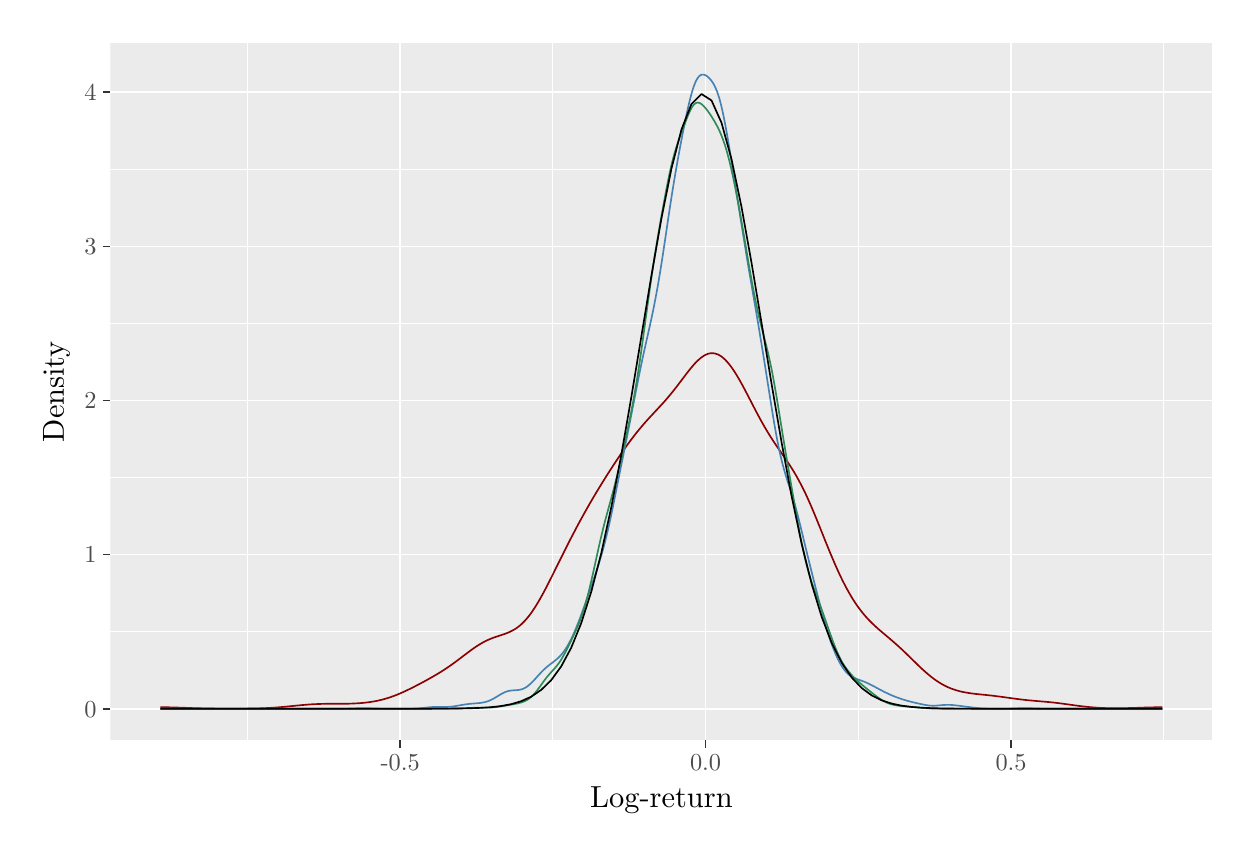
\begin{tikzpicture}[x=1pt,y=1pt]
\definecolor{fillColor}{RGB}{255,255,255}
\path[use as bounding box,fill=fillColor,fill opacity=0.00] (0,0) rectangle (433.62,289.08);
\begin{scope}
\path[clip] (  0.00,  0.00) rectangle (433.62,289.08);
\definecolor{drawColor}{RGB}{255,255,255}
\definecolor{fillColor}{RGB}{255,255,255}

\path[draw=drawColor,line width= 0.6pt,line join=round,line cap=round,fill=fillColor] (  0.00,  0.00) rectangle (433.62,289.08);
\end{scope}
\begin{scope}
\path[clip] ( 29.87, 31.53) rectangle (428.12,283.58);
\definecolor{fillColor}{gray}{0.92}

\path[fill=fillColor] ( 29.87, 31.53) rectangle (428.12,283.58);
\definecolor{drawColor}{RGB}{255,255,255}

\path[draw=drawColor,line width= 0.3pt,line join=round] ( 29.87, 70.83) --
	(428.12, 70.83);

\path[draw=drawColor,line width= 0.3pt,line join=round] ( 29.87,126.52) --
	(428.12,126.52);

\path[draw=drawColor,line width= 0.3pt,line join=round] ( 29.87,182.21) --
	(428.12,182.21);

\path[draw=drawColor,line width= 0.3pt,line join=round] ( 29.87,237.89) --
	(428.12,237.89);

\path[draw=drawColor,line width= 0.3pt,line join=round] ( 79.41, 31.53) --
	( 79.41,283.58);

\path[draw=drawColor,line width= 0.3pt,line join=round] (189.78, 31.53) --
	(189.78,283.58);

\path[draw=drawColor,line width= 0.3pt,line join=round] (300.16, 31.53) --
	(300.16,283.58);

\path[draw=drawColor,line width= 0.3pt,line join=round] (410.53, 31.53) --
	(410.53,283.58);

\path[draw=drawColor,line width= 0.6pt,line join=round] ( 29.87, 42.99) --
	(428.12, 42.99);

\path[draw=drawColor,line width= 0.6pt,line join=round] ( 29.87, 98.67) --
	(428.12, 98.67);

\path[draw=drawColor,line width= 0.6pt,line join=round] ( 29.87,154.36) --
	(428.12,154.36);

\path[draw=drawColor,line width= 0.6pt,line join=round] ( 29.87,210.05) --
	(428.12,210.05);

\path[draw=drawColor,line width= 0.6pt,line join=round] ( 29.87,265.74) --
	(428.12,265.74);

\path[draw=drawColor,line width= 0.6pt,line join=round] (134.60, 31.53) --
	(134.60,283.58);

\path[draw=drawColor,line width= 0.6pt,line join=round] (244.97, 31.53) --
	(244.97,283.58);

\path[draw=drawColor,line width= 0.6pt,line join=round] (355.35, 31.53) --
	(355.35,283.58);
\definecolor{drawColor}{RGB}{139,0,0}

\path[draw=drawColor,line width= 0.6pt,line join=round] ( 47.97, 43.52) --
	( 48.68, 43.52) --
	( 49.39, 43.51) --
	( 50.10, 43.50) --
	( 50.81, 43.49) --
	( 51.51, 43.48) --
	( 52.22, 43.46) --
	( 52.93, 43.44) --
	( 53.64, 43.42) --
	( 54.35, 43.40) --
	( 55.06, 43.37) --
	( 55.76, 43.35) --
	( 56.47, 43.32) --
	( 57.18, 43.30) --
	( 57.89, 43.27) --
	( 58.60, 43.25) --
	( 59.31, 43.22) --
	( 60.02, 43.20) --
	( 60.72, 43.18) --
	( 61.43, 43.16) --
	( 62.14, 43.14) --
	( 62.85, 43.12) --
	( 63.56, 43.10) --
	( 64.27, 43.09) --
	( 64.98, 43.07) --
	( 65.68, 43.06) --
	( 66.39, 43.05) --
	( 67.10, 43.04) --
	( 67.81, 43.03) --
	( 68.52, 43.02) --
	( 69.23, 43.02) --
	( 69.93, 43.01) --
	( 70.64, 43.01) --
	( 71.35, 43.01) --
	( 72.06, 43.00) --
	( 72.77, 43.00) --
	( 73.48, 43.00) --
	( 74.19, 43.00) --
	( 74.89, 43.00) --
	( 75.60, 43.00) --
	( 76.31, 43.01) --
	( 77.02, 43.01) --
	( 77.73, 43.01) --
	( 78.44, 43.02) --
	( 79.15, 43.03) --
	( 79.85, 43.04) --
	( 80.56, 43.05) --
	( 81.27, 43.06) --
	( 81.98, 43.07) --
	( 82.69, 43.09) --
	( 83.40, 43.11) --
	( 84.10, 43.13) --
	( 84.81, 43.15) --
	( 85.52, 43.18) --
	( 86.23, 43.21) --
	( 86.94, 43.25) --
	( 87.65, 43.29) --
	( 88.36, 43.33) --
	( 89.06, 43.37) --
	( 89.77, 43.42) --
	( 90.48, 43.48) --
	( 91.19, 43.54) --
	( 91.90, 43.60) --
	( 92.61, 43.66) --
	( 93.32, 43.73) --
	( 94.02, 43.80) --
	( 94.73, 43.87) --
	( 95.44, 43.94) --
	( 96.15, 44.01) --
	( 96.86, 44.08) --
	( 97.57, 44.15) --
	( 98.28, 44.22) --
	( 98.98, 44.29) --
	( 99.69, 44.35) --
	(100.40, 44.41) --
	(101.11, 44.47) --
	(101.82, 44.52) --
	(102.53, 44.57) --
	(103.23, 44.61) --
	(103.94, 44.64) --
	(104.65, 44.67) --
	(105.36, 44.70) --
	(106.07, 44.72) --
	(106.78, 44.74) --
	(107.49, 44.75) --
	(108.19, 44.75) --
	(108.90, 44.76) --
	(109.61, 44.76) --
	(110.32, 44.76) --
	(111.03, 44.76) --
	(111.74, 44.76) --
	(112.45, 44.76) --
	(113.15, 44.76) --
	(113.86, 44.77) --
	(114.57, 44.78) --
	(115.28, 44.79) --
	(115.99, 44.80) --
	(116.70, 44.82) --
	(117.40, 44.85) --
	(118.11, 44.88) --
	(118.82, 44.92) --
	(119.53, 44.96) --
	(120.24, 45.01) --
	(120.95, 45.07) --
	(121.66, 45.14) --
	(122.36, 45.22) --
	(123.07, 45.31) --
	(123.78, 45.41) --
	(124.49, 45.52) --
	(125.20, 45.64) --
	(125.91, 45.77) --
	(126.62, 45.92) --
	(127.32, 46.08) --
	(128.03, 46.25) --
	(128.74, 46.44) --
	(129.45, 46.64) --
	(130.16, 46.86) --
	(130.87, 47.09) --
	(131.57, 47.33) --
	(132.28, 47.59) --
	(132.99, 47.86) --
	(133.70, 48.14) --
	(134.41, 48.44) --
	(135.12, 48.75) --
	(135.83, 49.07) --
	(136.53, 49.39) --
	(137.24, 49.73) --
	(137.95, 50.07) --
	(138.66, 50.42) --
	(139.37, 50.78) --
	(140.08, 51.14) --
	(140.79, 51.51) --
	(141.49, 51.88) --
	(142.20, 52.25) --
	(142.91, 52.63) --
	(143.62, 53.02) --
	(144.33, 53.40) --
	(145.04, 53.80) --
	(145.74, 54.19) --
	(146.45, 54.60) --
	(147.16, 55.01) --
	(147.87, 55.43) --
	(148.58, 55.85) --
	(149.29, 56.29) --
	(150.00, 56.74) --
	(150.70, 57.20) --
	(151.41, 57.67) --
	(152.12, 58.15) --
	(152.83, 58.64) --
	(153.54, 59.14) --
	(154.25, 59.66) --
	(154.96, 60.18) --
	(155.66, 60.71) --
	(156.37, 61.25) --
	(157.08, 61.79) --
	(157.79, 62.33) --
	(158.50, 62.86) --
	(159.21, 63.40) --
	(159.92, 63.92) --
	(160.62, 64.44) --
	(161.33, 64.94) --
	(162.04, 65.42) --
	(162.75, 65.88) --
	(163.46, 66.32) --
	(164.17, 66.74) --
	(164.87, 67.12) --
	(165.58, 67.48) --
	(166.29, 67.82) --
	(167.00, 68.13) --
	(167.71, 68.42) --
	(168.42, 68.69) --
	(169.13, 68.93) --
	(169.83, 69.17) --
	(170.54, 69.40) --
	(171.25, 69.64) --
	(171.96, 69.87) --
	(172.67, 70.12) --
	(173.38, 70.39) --
	(174.09, 70.70) --
	(174.79, 71.03) --
	(175.50, 71.41) --
	(176.21, 71.83) --
	(176.92, 72.31) --
	(177.63, 72.85) --
	(178.34, 73.46) --
	(179.04, 74.13) --
	(179.75, 74.87) --
	(180.46, 75.68) --
	(181.17, 76.55) --
	(181.88, 77.50) --
	(182.59, 78.52) --
	(183.30, 79.60) --
	(184.00, 80.73) --
	(184.71, 81.92) --
	(185.42, 83.15) --
	(186.13, 84.44) --
	(186.84, 85.76) --
	(187.55, 87.12) --
	(188.26, 88.50) --
	(188.96, 89.90) --
	(189.67, 91.31) --
	(190.38, 92.74) --
	(191.09, 94.18) --
	(191.80, 95.61) --
	(192.51, 97.04) --
	(193.21, 98.47) --
	(193.92, 99.89) --
	(194.63,101.31) --
	(195.34,102.70) --
	(196.05,104.09) --
	(196.76,105.47) --
	(197.47,106.82) --
	(198.17,108.17) --
	(198.88,109.50) --
	(199.59,110.81) --
	(200.30,112.10) --
	(201.01,113.39) --
	(201.72,114.65) --
	(202.43,115.90) --
	(203.13,117.14) --
	(203.84,118.36) --
	(204.55,119.56) --
	(205.26,120.76) --
	(205.97,121.94) --
	(206.68,123.10) --
	(207.39,124.26) --
	(208.09,125.40) --
	(208.80,126.53) --
	(209.51,127.65) --
	(210.22,128.76) --
	(210.93,129.86) --
	(211.64,130.95) --
	(212.34,132.02) --
	(213.05,133.09) --
	(213.76,134.14) --
	(214.47,135.18) --
	(215.18,136.20) --
	(215.89,137.21) --
	(216.60,138.20) --
	(217.30,139.18) --
	(218.01,140.13) --
	(218.72,141.07) --
	(219.43,141.99) --
	(220.14,142.88) --
	(220.85,143.76) --
	(221.56,144.61) --
	(222.26,145.44) --
	(222.97,146.26) --
	(223.68,147.05) --
	(224.39,147.84) --
	(225.10,148.61) --
	(225.81,149.37) --
	(226.51,150.13) --
	(227.22,150.88) --
	(227.93,151.64) --
	(228.64,152.41) --
	(229.35,153.18) --
	(230.06,153.97) --
	(230.77,154.78) --
	(231.47,155.60) --
	(232.18,156.45) --
	(232.89,157.31) --
	(233.60,158.20) --
	(234.31,159.10) --
	(235.02,160.02) --
	(235.73,160.96) --
	(236.43,161.89) --
	(237.14,162.83) --
	(237.85,163.77) --
	(238.56,164.69) --
	(239.27,165.58) --
	(239.98,166.44) --
	(240.68,167.27) --
	(241.39,168.05) --
	(242.10,168.76) --
	(242.81,169.40) --
	(243.52,169.97) --
	(244.23,170.45) --
	(244.94,170.85) --
	(245.64,171.16) --
	(246.35,171.37) --
	(247.06,171.45) --
	(247.77,171.43) --
	(248.48,171.31) --
	(249.19,171.08) --
	(249.90,170.75) --
	(250.60,170.32) --
	(251.31,169.76) --
	(252.02,169.11) --
	(252.73,168.36) --
	(253.44,167.52) --
	(254.15,166.61) --
	(254.85,165.61) --
	(255.56,164.53) --
	(256.27,163.39) --
	(256.98,162.19) --
	(257.69,160.94) --
	(258.40,159.65) --
	(259.11,158.33) --
	(259.81,156.98) --
	(260.52,155.61) --
	(261.23,154.24) --
	(261.94,152.87) --
	(262.65,151.50) --
	(263.36,150.14) --
	(264.07,148.81) --
	(264.77,147.50) --
	(265.48,146.23) --
	(266.19,144.98) --
	(266.90,143.77) --
	(267.61,142.59) --
	(268.32,141.45) --
	(269.03,140.34) --
	(269.73,139.26) --
	(270.44,138.20) --
	(271.15,137.16) --
	(271.86,136.14) --
	(272.57,135.12) --
	(273.28,134.10) --
	(273.98,133.07) --
	(274.69,132.02) --
	(275.40,130.94) --
	(276.11,129.84) --
	(276.82,128.69) --
	(277.53,127.49) --
	(278.24,126.24) --
	(278.94,124.94) --
	(279.65,123.58) --
	(280.36,122.17) --
	(281.07,120.70) --
	(281.78,119.17) --
	(282.49,117.58) --
	(283.20,115.96) --
	(283.90,114.29) --
	(284.61,112.59) --
	(285.32,110.85) --
	(286.03,109.10) --
	(286.74,107.33) --
	(287.45,105.56) --
	(288.15,103.79) --
	(288.86,102.04) --
	(289.57,100.30) --
	(290.28, 98.59) --
	(290.99, 96.91) --
	(291.70, 95.27) --
	(292.41, 93.66) --
	(293.11, 92.11) --
	(293.82, 90.60) --
	(294.53, 89.15) --
	(295.24, 87.76) --
	(295.95, 86.42) --
	(296.66, 85.14) --
	(297.37, 83.91) --
	(298.07, 82.74) --
	(298.78, 81.63) --
	(299.49, 80.58) --
	(300.20, 79.58) --
	(300.91, 78.63) --
	(301.62, 77.72) --
	(302.32, 76.87) --
	(303.03, 76.06) --
	(303.74, 75.29) --
	(304.45, 74.55) --
	(305.16, 73.85) --
	(305.87, 73.17) --
	(306.58, 72.52) --
	(307.28, 71.88) --
	(307.99, 71.27) --
	(308.70, 70.66) --
	(309.41, 70.06) --
	(310.12, 69.47) --
	(310.83, 68.87) --
	(311.54, 68.27) --
	(312.24, 67.67) --
	(312.95, 67.05) --
	(313.66, 66.43) --
	(314.37, 65.80) --
	(315.08, 65.15) --
	(315.79, 64.50) --
	(316.49, 63.83) --
	(317.20, 63.15) --
	(317.91, 62.46) --
	(318.62, 61.77) --
	(319.33, 61.08) --
	(320.04, 60.38) --
	(320.75, 59.69) --
	(321.45, 59.00) --
	(322.16, 58.32) --
	(322.87, 57.65) --
	(323.58, 57.00) --
	(324.29, 56.36) --
	(325.00, 55.74) --
	(325.71, 55.15) --
	(326.41, 54.57) --
	(327.12, 54.02) --
	(327.83, 53.50) --
	(328.54, 53.01) --
	(329.25, 52.54) --
	(329.96, 52.11) --
	(330.67, 51.70) --
	(331.37, 51.33) --
	(332.08, 50.98) --
	(332.79, 50.65) --
	(333.50, 50.36) --
	(334.21, 50.09) --
	(334.92, 49.85) --
	(335.62, 49.63) --
	(336.33, 49.42) --
	(337.04, 49.24) --
	(337.75, 49.08) --
	(338.46, 48.94) --
	(339.17, 48.81) --
	(339.88, 48.69) --
	(340.58, 48.58) --
	(341.29, 48.48) --
	(342.00, 48.40) --
	(342.71, 48.31) --
	(343.42, 48.24) --
	(344.13, 48.16) --
	(344.84, 48.09) --
	(345.54, 48.02) --
	(346.25, 47.95) --
	(346.96, 47.87) --
	(347.67, 47.80) --
	(348.38, 47.72) --
	(349.09, 47.64) --
	(349.79, 47.55) --
	(350.50, 47.46) --
	(351.21, 47.37) --
	(351.92, 47.28) --
	(352.63, 47.18) --
	(353.34, 47.08) --
	(354.05, 46.98) --
	(354.75, 46.88) --
	(355.46, 46.78) --
	(356.17, 46.69) --
	(356.88, 46.59) --
	(357.59, 46.50) --
	(358.30, 46.41) --
	(359.01, 46.32) --
	(359.71, 46.24) --
	(360.42, 46.16) --
	(361.13, 46.09) --
	(361.84, 46.02) --
	(362.55, 45.95) --
	(363.26, 45.89) --
	(363.96, 45.82) --
	(364.67, 45.76) --
	(365.38, 45.70) --
	(366.09, 45.64) --
	(366.80, 45.58) --
	(367.51, 45.52) --
	(368.22, 45.46) --
	(368.92, 45.39) --
	(369.63, 45.32) --
	(370.34, 45.25) --
	(371.05, 45.17) --
	(371.76, 45.09) --
	(372.47, 45.00) --
	(373.18, 44.91) --
	(373.88, 44.82) --
	(374.59, 44.72) --
	(375.30, 44.63) --
	(376.01, 44.53) --
	(376.72, 44.43) --
	(377.43, 44.33) --
	(378.13, 44.23) --
	(378.84, 44.14) --
	(379.55, 44.04) --
	(380.26, 43.95) --
	(380.97, 43.86) --
	(381.68, 43.78) --
	(382.39, 43.70) --
	(383.09, 43.63) --
	(383.80, 43.56) --
	(384.51, 43.50) --
	(385.22, 43.44) --
	(385.93, 43.39) --
	(386.64, 43.34) --
	(387.35, 43.30) --
	(388.05, 43.26) --
	(388.76, 43.23) --
	(389.47, 43.21) --
	(390.18, 43.19) --
	(390.89, 43.17) --
	(391.60, 43.16) --
	(392.31, 43.15) --
	(393.01, 43.15) --
	(393.72, 43.15) --
	(394.43, 43.15) --
	(395.14, 43.16) --
	(395.85, 43.17) --
	(396.56, 43.18) --
	(397.26, 43.20) --
	(397.97, 43.22) --
	(398.68, 43.24) --
	(399.39, 43.26) --
	(400.10, 43.28) --
	(400.81, 43.30) --
	(401.52, 43.33) --
	(402.22, 43.35) --
	(402.93, 43.38) --
	(403.64, 43.40) --
	(404.35, 43.42) --
	(405.06, 43.44) --
	(405.77, 43.46) --
	(406.48, 43.48) --
	(407.18, 43.49) --
	(407.89, 43.50) --
	(408.60, 43.51) --
	(409.31, 43.52) --
	(410.02, 43.52);
\definecolor{drawColor}{RGB}{70,130,180}

\path[draw=drawColor,line width= 0.6pt,line join=round] ( 47.97, 42.99) --
	( 48.68, 42.99) --
	( 49.39, 42.99) --
	( 50.10, 42.99) --
	( 50.81, 42.99) --
	( 51.51, 42.99) --
	( 52.22, 42.99) --
	( 52.93, 42.99) --
	( 53.64, 42.99) --
	( 54.35, 42.99) --
	( 55.06, 42.99) --
	( 55.76, 42.99) --
	( 56.47, 42.99) --
	( 57.18, 42.99) --
	( 57.89, 42.99) --
	( 58.60, 42.99) --
	( 59.31, 42.99) --
	( 60.02, 42.99) --
	( 60.72, 42.99) --
	( 61.43, 42.99) --
	( 62.14, 42.99) --
	( 62.85, 42.99) --
	( 63.56, 42.99) --
	( 64.27, 42.99) --
	( 64.98, 42.99) --
	( 65.68, 42.99) --
	( 66.39, 42.99) --
	( 67.10, 42.99) --
	( 67.81, 42.99) --
	( 68.52, 42.99) --
	( 69.23, 42.99) --
	( 69.93, 42.99) --
	( 70.64, 42.99) --
	( 71.35, 42.99) --
	( 72.06, 42.99) --
	( 72.77, 42.99) --
	( 73.48, 42.99) --
	( 74.19, 42.99) --
	( 74.89, 42.99) --
	( 75.60, 42.99) --
	( 76.31, 42.99) --
	( 77.02, 42.99) --
	( 77.73, 42.99) --
	( 78.44, 42.99) --
	( 79.15, 42.99) --
	( 79.85, 42.99) --
	( 80.56, 42.99) --
	( 81.27, 42.99) --
	( 81.98, 42.99) --
	( 82.69, 42.99) --
	( 83.40, 42.99) --
	( 84.10, 42.99) --
	( 84.81, 42.99) --
	( 85.52, 42.99) --
	( 86.23, 42.99) --
	( 86.94, 42.99) --
	( 87.65, 42.99) --
	( 88.36, 42.99) --
	( 89.06, 42.99) --
	( 89.77, 42.99) --
	( 90.48, 42.99) --
	( 91.19, 42.99) --
	( 91.90, 42.99) --
	( 92.61, 42.99) --
	( 93.32, 42.99) --
	( 94.02, 42.99) --
	( 94.73, 42.99) --
	( 95.44, 42.99) --
	( 96.15, 42.99) --
	( 96.86, 42.99) --
	( 97.57, 42.99) --
	( 98.28, 42.99) --
	( 98.98, 42.99) --
	( 99.69, 42.99) --
	(100.40, 42.99) --
	(101.11, 42.99) --
	(101.82, 42.99) --
	(102.53, 42.99) --
	(103.23, 42.99) --
	(103.94, 42.99) --
	(104.65, 42.99) --
	(105.36, 42.99) --
	(106.07, 42.99) --
	(106.78, 42.99) --
	(107.49, 42.99) --
	(108.19, 42.99) --
	(108.90, 42.99) --
	(109.61, 42.99) --
	(110.32, 42.99) --
	(111.03, 42.99) --
	(111.74, 42.99) --
	(112.45, 42.99) --
	(113.15, 43.00) --
	(113.86, 43.00) --
	(114.57, 43.01) --
	(115.28, 43.02) --
	(115.99, 43.04) --
	(116.70, 43.06) --
	(117.40, 43.08) --
	(118.11, 43.10) --
	(118.82, 43.13) --
	(119.53, 43.15) --
	(120.24, 43.17) --
	(120.95, 43.17) --
	(121.66, 43.18) --
	(122.36, 43.17) --
	(123.07, 43.15) --
	(123.78, 43.13) --
	(124.49, 43.11) --
	(125.20, 43.08) --
	(125.91, 43.06) --
	(126.62, 43.04) --
	(127.32, 43.02) --
	(128.03, 43.01) --
	(128.74, 43.00) --
	(129.45, 43.00) --
	(130.16, 42.99) --
	(130.87, 42.99) --
	(131.57, 42.99) --
	(132.28, 42.99) --
	(132.99, 42.99) --
	(133.70, 42.99) --
	(134.41, 42.99) --
	(135.12, 42.99) --
	(135.83, 42.99) --
	(136.53, 42.99) --
	(137.24, 43.00) --
	(137.95, 43.00) --
	(138.66, 43.01) --
	(139.37, 43.03) --
	(140.08, 43.06) --
	(140.79, 43.09) --
	(141.49, 43.14) --
	(142.20, 43.20) --
	(142.91, 43.27) --
	(143.62, 43.34) --
	(144.33, 43.42) --
	(145.04, 43.49) --
	(145.74, 43.55) --
	(146.45, 43.60) --
	(147.16, 43.62) --
	(147.87, 43.63) --
	(148.58, 43.62) --
	(149.29, 43.61) --
	(150.00, 43.60) --
	(150.70, 43.60) --
	(151.41, 43.61) --
	(152.12, 43.65) --
	(152.83, 43.70) --
	(153.54, 43.78) --
	(154.25, 43.88) --
	(154.96, 44.00) --
	(155.66, 44.12) --
	(156.37, 44.25) --
	(157.08, 44.37) --
	(157.79, 44.49) --
	(158.50, 44.59) --
	(159.21, 44.68) --
	(159.92, 44.76) --
	(160.62, 44.82) --
	(161.33, 44.88) --
	(162.04, 44.93) --
	(162.75, 44.99) --
	(163.46, 45.06) --
	(164.17, 45.16) --
	(164.87, 45.30) --
	(165.58, 45.47) --
	(166.29, 45.70) --
	(167.00, 45.98) --
	(167.71, 46.32) --
	(168.42, 46.69) --
	(169.13, 47.10) --
	(169.83, 47.53) --
	(170.54, 47.96) --
	(171.25, 48.37) --
	(171.96, 48.74) --
	(172.67, 49.05) --
	(173.38, 49.29) --
	(174.09, 49.46) --
	(174.79, 49.57) --
	(175.50, 49.63) --
	(176.21, 49.67) --
	(176.92, 49.71) --
	(177.63, 49.79) --
	(178.34, 49.95) --
	(179.04, 50.19) --
	(179.75, 50.53) --
	(180.46, 50.99) --
	(181.17, 51.54) --
	(181.88, 52.18) --
	(182.59, 52.89) --
	(183.30, 53.65) --
	(184.00, 54.43) --
	(184.71, 55.21) --
	(185.42, 55.98) --
	(186.13, 56.71) --
	(186.84, 57.39) --
	(187.55, 58.02) --
	(188.26, 58.60) --
	(188.96, 59.15) --
	(189.67, 59.68) --
	(190.38, 60.23) --
	(191.09, 60.80) --
	(191.80, 61.43) --
	(192.51, 62.15) --
	(193.21, 62.97) --
	(193.92, 63.90) --
	(194.63, 64.96) --
	(195.34, 66.16) --
	(196.05, 67.48) --
	(196.76, 68.91) --
	(197.47, 70.47) --
	(198.17, 72.13) --
	(198.88, 73.89) --
	(199.59, 75.74) --
	(200.30, 77.66) --
	(201.01, 79.63) --
	(201.72, 81.64) --
	(202.43, 83.68) --
	(203.13, 85.72) --
	(203.84, 87.77) --
	(204.55, 89.84) --
	(205.26, 91.94) --
	(205.97, 94.10) --
	(206.68, 96.35) --
	(207.39, 98.72) --
	(208.09,101.25) --
	(208.80,103.97) --
	(209.51,106.90) --
	(210.22,110.01) --
	(210.93,113.30) --
	(211.64,116.73) --
	(212.34,120.24) --
	(213.05,123.80) --
	(213.76,127.36) --
	(214.47,130.89) --
	(215.18,134.40) --
	(215.89,137.90) --
	(216.60,141.42) --
	(217.30,144.98) --
	(218.01,148.59) --
	(218.72,152.25) --
	(219.43,155.92) --
	(220.14,159.56) --
	(220.85,163.12) --
	(221.56,166.57) --
	(222.26,169.91) --
	(222.97,173.14) --
	(223.68,176.30) --
	(224.39,179.44) --
	(225.10,182.63) --
	(225.81,185.94) --
	(226.51,189.44) --
	(227.22,193.16) --
	(227.93,197.16) --
	(228.64,201.43) --
	(229.35,205.94) --
	(230.06,210.64) --
	(230.77,215.42) --
	(231.47,220.19) --
	(232.18,224.88) --
	(232.89,229.43) --
	(233.60,233.80) --
	(234.31,237.97) --
	(235.02,241.98) --
	(235.73,245.83) --
	(236.43,249.55) --
	(237.14,253.15) --
	(237.85,256.62) --
	(238.56,259.90) --
	(239.27,262.93) --
	(239.98,265.61) --
	(240.68,267.85) --
	(241.39,269.62) --
	(242.10,270.90) --
	(242.81,271.71) --
	(243.52,272.09) --
	(244.23,272.12) --
	(244.94,271.88) --
	(245.64,271.42) --
	(246.35,270.77) --
	(247.06,269.94) --
	(247.77,268.88) --
	(248.48,267.53) --
	(249.19,265.81) --
	(249.90,263.66) --
	(250.60,260.99) --
	(251.31,257.86) --
	(252.02,254.30) --
	(252.73,250.39) --
	(253.44,246.23) --
	(254.15,241.90) --
	(254.85,237.48) --
	(255.56,233.00) --
	(256.27,228.50) --
	(256.98,224.01) --
	(257.69,219.54) --
	(258.40,215.10) --
	(259.11,210.72) --
	(259.81,206.40) --
	(260.52,202.17) --
	(261.23,198.01) --
	(261.94,193.89) --
	(262.65,189.78) --
	(263.36,185.65) --
	(264.07,181.47) --
	(264.77,177.22) --
	(265.48,172.89) --
	(266.19,168.48) --
	(266.90,164.00) --
	(267.61,159.49) --
	(268.32,155.00) --
	(269.03,150.57) --
	(269.73,146.30) --
	(270.44,142.25) --
	(271.15,138.52) --
	(271.86,135.17) --
	(272.57,132.18) --
	(273.28,129.52) --
	(273.98,127.12) --
	(274.69,124.88) --
	(275.40,122.70) --
	(276.11,120.47) --
	(276.82,118.12) --
	(277.53,115.62) --
	(278.24,112.96) --
	(278.94,110.17) --
	(279.65,107.27) --
	(280.36,104.33) --
	(281.07,101.39) --
	(281.78, 98.47) --
	(282.49, 95.59) --
	(283.20, 92.75) --
	(283.90, 89.94) --
	(284.61, 87.14) --
	(285.32, 84.36) --
	(286.03, 81.62) --
	(286.74, 78.92) --
	(287.45, 76.30) --
	(288.15, 73.78) --
	(288.86, 71.38) --
	(289.57, 69.13) --
	(290.28, 67.03) --
	(290.99, 65.09) --
	(291.70, 63.31) --
	(292.41, 61.69) --
	(293.11, 60.23) --
	(293.82, 58.93) --
	(294.53, 57.79) --
	(295.24, 56.82) --
	(295.95, 56.01) --
	(296.66, 55.34) --
	(297.37, 54.81) --
	(298.07, 54.38) --
	(298.78, 54.04) --
	(299.49, 53.75) --
	(300.20, 53.50) --
	(300.91, 53.25) --
	(301.62, 52.99) --
	(302.32, 52.72) --
	(303.03, 52.42) --
	(303.74, 52.09) --
	(304.45, 51.75) --
	(305.16, 51.39) --
	(305.87, 51.02) --
	(306.58, 50.64) --
	(307.28, 50.26) --
	(307.99, 49.88) --
	(308.70, 49.51) --
	(309.41, 49.14) --
	(310.12, 48.79) --
	(310.83, 48.45) --
	(311.54, 48.12) --
	(312.24, 47.81) --
	(312.95, 47.52) --
	(313.66, 47.24) --
	(314.37, 46.98) --
	(315.08, 46.73) --
	(315.79, 46.49) --
	(316.49, 46.26) --
	(317.20, 46.05) --
	(317.91, 45.84) --
	(318.62, 45.64) --
	(319.33, 45.46) --
	(320.04, 45.29) --
	(320.75, 45.12) --
	(321.45, 44.96) --
	(322.16, 44.80) --
	(322.87, 44.65) --
	(323.58, 44.50) --
	(324.29, 44.36) --
	(325.00, 44.24) --
	(325.71, 44.15) --
	(326.41, 44.09) --
	(327.12, 44.07) --
	(327.83, 44.08) --
	(328.54, 44.12) --
	(329.25, 44.18) --
	(329.96, 44.25) --
	(330.67, 44.31) --
	(331.37, 44.35) --
	(332.08, 44.38) --
	(332.79, 44.38) --
	(333.50, 44.36) --
	(334.21, 44.31) --
	(334.92, 44.24) --
	(335.62, 44.16) --
	(336.33, 44.08) --
	(337.04, 43.99) --
	(337.75, 43.90) --
	(338.46, 43.80) --
	(339.17, 43.71) --
	(339.88, 43.62) --
	(340.58, 43.53) --
	(341.29, 43.44) --
	(342.00, 43.36) --
	(342.71, 43.28) --
	(343.42, 43.21) --
	(344.13, 43.15) --
	(344.84, 43.10) --
	(345.54, 43.07) --
	(346.25, 43.04) --
	(346.96, 43.02) --
	(347.67, 43.01) --
	(348.38, 43.00) --
	(349.09, 42.99) --
	(349.79, 42.99) --
	(350.50, 42.99) --
	(351.21, 42.99) --
	(351.92, 43.00) --
	(352.63, 43.00) --
	(353.34, 43.01) --
	(354.05, 43.02) --
	(354.75, 43.03) --
	(355.46, 43.05) --
	(356.17, 43.07) --
	(356.88, 43.10) --
	(357.59, 43.12) --
	(358.30, 43.14) --
	(359.01, 43.16) --
	(359.71, 43.17) --
	(360.42, 43.18) --
	(361.13, 43.17) --
	(361.84, 43.16) --
	(362.55, 43.14) --
	(363.26, 43.12) --
	(363.96, 43.09) --
	(364.67, 43.07) --
	(365.38, 43.05) --
	(366.09, 43.03) --
	(366.80, 43.02) --
	(367.51, 43.01) --
	(368.22, 43.00) --
	(368.92, 42.99) --
	(369.63, 42.99) --
	(370.34, 42.99) --
	(371.05, 42.99) --
	(371.76, 42.99) --
	(372.47, 42.99) --
	(373.18, 42.99) --
	(373.88, 42.99) --
	(374.59, 42.99) --
	(375.30, 42.99) --
	(376.01, 42.99) --
	(376.72, 42.99) --
	(377.43, 42.99) --
	(378.13, 42.99) --
	(378.84, 42.99) --
	(379.55, 42.99) --
	(380.26, 42.99) --
	(380.97, 42.99) --
	(381.68, 42.99) --
	(382.39, 42.99) --
	(383.09, 42.99) --
	(383.80, 42.99) --
	(384.51, 42.99) --
	(385.22, 42.99) --
	(385.93, 42.99) --
	(386.64, 42.99) --
	(387.35, 42.99) --
	(388.05, 42.99) --
	(388.76, 42.99) --
	(389.47, 42.99) --
	(390.18, 42.99) --
	(390.89, 42.99) --
	(391.60, 42.99) --
	(392.31, 42.99) --
	(393.01, 42.99) --
	(393.72, 42.99) --
	(394.43, 42.99) --
	(395.14, 42.99) --
	(395.85, 42.99) --
	(396.56, 42.99) --
	(397.26, 42.99) --
	(397.97, 42.99) --
	(398.68, 42.99) --
	(399.39, 42.99) --
	(400.10, 42.99) --
	(400.81, 42.99) --
	(401.52, 42.99) --
	(402.22, 42.99) --
	(402.93, 42.99) --
	(403.64, 42.99) --
	(404.35, 42.99) --
	(405.06, 42.99) --
	(405.77, 42.99) --
	(406.48, 42.99) --
	(407.18, 42.99) --
	(407.89, 42.99) --
	(408.60, 42.99) --
	(409.31, 42.99) --
	(410.02, 42.99);
\definecolor{drawColor}{RGB}{46,139,87}

\path[draw=drawColor,line width= 0.6pt,line join=round] ( 47.97, 42.99) --
	( 48.68, 42.99) --
	( 49.39, 42.99) --
	( 50.10, 42.99) --
	( 50.81, 42.99) --
	( 51.51, 42.99) --
	( 52.22, 42.99) --
	( 52.93, 42.99) --
	( 53.64, 42.99) --
	( 54.35, 42.99) --
	( 55.06, 42.99) --
	( 55.76, 42.99) --
	( 56.47, 42.99) --
	( 57.18, 42.99) --
	( 57.89, 42.99) --
	( 58.60, 42.99) --
	( 59.31, 42.99) --
	( 60.02, 42.99) --
	( 60.72, 42.99) --
	( 61.43, 42.99) --
	( 62.14, 42.99) --
	( 62.85, 42.99) --
	( 63.56, 42.99) --
	( 64.27, 42.99) --
	( 64.98, 42.99) --
	( 65.68, 42.99) --
	( 66.39, 42.99) --
	( 67.10, 42.99) --
	( 67.81, 42.99) --
	( 68.52, 42.99) --
	( 69.23, 42.99) --
	( 69.93, 42.99) --
	( 70.64, 42.99) --
	( 71.35, 42.99) --
	( 72.06, 42.99) --
	( 72.77, 42.99) --
	( 73.48, 42.99) --
	( 74.19, 42.99) --
	( 74.89, 42.99) --
	( 75.60, 42.99) --
	( 76.31, 42.99) --
	( 77.02, 42.99) --
	( 77.73, 42.99) --
	( 78.44, 42.99) --
	( 79.15, 42.99) --
	( 79.85, 42.99) --
	( 80.56, 42.99) --
	( 81.27, 42.99) --
	( 81.98, 42.99) --
	( 82.69, 42.99) --
	( 83.40, 42.99) --
	( 84.10, 42.99) --
	( 84.81, 42.99) --
	( 85.52, 42.99) --
	( 86.23, 42.99) --
	( 86.94, 42.99) --
	( 87.65, 42.99) --
	( 88.36, 42.99) --
	( 89.06, 42.99) --
	( 89.77, 42.99) --
	( 90.48, 42.99) --
	( 91.19, 42.99) --
	( 91.90, 42.99) --
	( 92.61, 42.99) --
	( 93.32, 42.99) --
	( 94.02, 42.99) --
	( 94.73, 42.99) --
	( 95.44, 42.99) --
	( 96.15, 42.99) --
	( 96.86, 42.99) --
	( 97.57, 42.99) --
	( 98.28, 42.99) --
	( 98.98, 42.99) --
	( 99.69, 42.99) --
	(100.40, 42.99) --
	(101.11, 42.99) --
	(101.82, 42.99) --
	(102.53, 42.99) --
	(103.23, 42.99) --
	(103.94, 42.99) --
	(104.65, 42.99) --
	(105.36, 42.99) --
	(106.07, 42.99) --
	(106.78, 42.99) --
	(107.49, 42.99) --
	(108.19, 42.99) --
	(108.90, 42.99) --
	(109.61, 42.99) --
	(110.32, 42.99) --
	(111.03, 42.99) --
	(111.74, 42.99) --
	(112.45, 42.99) --
	(113.15, 42.99) --
	(113.86, 42.99) --
	(114.57, 42.99) --
	(115.28, 42.99) --
	(115.99, 42.99) --
	(116.70, 42.99) --
	(117.40, 42.99) --
	(118.11, 42.99) --
	(118.82, 42.99) --
	(119.53, 42.99) --
	(120.24, 42.99) --
	(120.95, 42.99) --
	(121.66, 42.99) --
	(122.36, 42.99) --
	(123.07, 42.99) --
	(123.78, 42.99) --
	(124.49, 42.99) --
	(125.20, 42.99) --
	(125.91, 42.99) --
	(126.62, 42.99) --
	(127.32, 42.99) --
	(128.03, 42.99) --
	(128.74, 42.99) --
	(129.45, 42.99) --
	(130.16, 42.99) --
	(130.87, 42.99) --
	(131.57, 42.99) --
	(132.28, 42.99) --
	(132.99, 42.99) --
	(133.70, 42.99) --
	(134.41, 42.99) --
	(135.12, 42.99) --
	(135.83, 42.99) --
	(136.53, 42.99) --
	(137.24, 42.99) --
	(137.95, 42.99) --
	(138.66, 42.99) --
	(139.37, 42.99) --
	(140.08, 42.99) --
	(140.79, 42.99) --
	(141.49, 42.99) --
	(142.20, 42.99) --
	(142.91, 42.99) --
	(143.62, 42.99) --
	(144.33, 42.99) --
	(145.04, 42.99) --
	(145.74, 42.99) --
	(146.45, 42.99) --
	(147.16, 42.99) --
	(147.87, 42.99) --
	(148.58, 42.99) --
	(149.29, 42.99) --
	(150.00, 42.99) --
	(150.70, 42.99) --
	(151.41, 43.00) --
	(152.12, 43.00) --
	(152.83, 43.01) --
	(153.54, 43.03) --
	(154.25, 43.04) --
	(154.96, 43.06) --
	(155.66, 43.09) --
	(156.37, 43.12) --
	(157.08, 43.15) --
	(157.79, 43.18) --
	(158.50, 43.21) --
	(159.21, 43.24) --
	(159.92, 43.27) --
	(160.62, 43.30) --
	(161.33, 43.32) --
	(162.04, 43.34) --
	(162.75, 43.36) --
	(163.46, 43.37) --
	(164.17, 43.37) --
	(164.87, 43.37) --
	(165.58, 43.37) --
	(166.29, 43.38) --
	(167.00, 43.40) --
	(167.71, 43.43) --
	(168.42, 43.49) --
	(169.13, 43.56) --
	(169.83, 43.65) --
	(170.54, 43.76) --
	(171.25, 43.87) --
	(171.96, 43.99) --
	(172.67, 44.12) --
	(173.38, 44.24) --
	(174.09, 44.37) --
	(174.79, 44.49) --
	(175.50, 44.61) --
	(176.21, 44.74) --
	(176.92, 44.88) --
	(177.63, 45.04) --
	(178.34, 45.24) --
	(179.04, 45.48) --
	(179.75, 45.77) --
	(180.46, 46.15) --
	(181.17, 46.61) --
	(181.88, 47.17) --
	(182.59, 47.85) --
	(183.30, 48.62) --
	(184.00, 49.49) --
	(184.71, 50.44) --
	(185.42, 51.42) --
	(186.13, 52.42) --
	(186.84, 53.39) --
	(187.55, 54.31) --
	(188.26, 55.16) --
	(188.96, 55.96) --
	(189.67, 56.74) --
	(190.38, 57.52) --
	(191.09, 58.35) --
	(191.80, 59.26) --
	(192.51, 60.29) --
	(193.21, 61.43) --
	(193.92, 62.69) --
	(194.63, 64.03) --
	(195.34, 65.45) --
	(196.05, 66.90) --
	(196.76, 68.38) --
	(197.47, 69.89) --
	(198.17, 71.45) --
	(198.88, 73.10) --
	(199.59, 74.88) --
	(200.30, 76.84) --
	(201.01, 79.01) --
	(201.72, 81.42) --
	(202.43, 84.06) --
	(203.13, 86.92) --
	(203.84, 89.96) --
	(204.55, 93.13) --
	(205.26, 96.36) --
	(205.97, 99.60) --
	(206.68,102.76) --
	(207.39,105.81) --
	(208.09,108.69) --
	(208.80,111.44) --
	(209.51,114.07) --
	(210.22,116.65) --
	(210.93,119.23) --
	(211.64,121.86) --
	(212.34,124.58) --
	(213.05,127.42) --
	(213.76,130.36) --
	(214.47,133.40) --
	(215.18,136.52) --
	(215.89,139.71) --
	(216.60,142.98) --
	(217.30,146.35) --
	(218.01,149.86) --
	(218.72,153.57) --
	(219.43,157.53) --
	(220.14,161.77) --
	(220.85,166.31) --
	(221.56,171.12) --
	(222.26,176.15) --
	(222.97,181.33) --
	(223.68,186.56) --
	(224.39,191.73) --
	(225.10,196.75) --
	(225.81,201.57) --
	(226.51,206.17) --
	(227.22,210.56) --
	(227.93,214.78) --
	(228.64,218.87) --
	(229.35,222.87) --
	(230.06,226.77) --
	(230.77,230.55) --
	(231.47,234.14) --
	(232.18,237.48) --
	(232.89,240.50) --
	(233.60,243.20) --
	(234.31,245.60) --
	(235.02,247.75) --
	(235.73,249.75) --
	(236.43,251.67) --
	(237.14,253.56) --
	(237.85,255.44) --
	(238.56,257.25) --
	(239.27,258.89) --
	(239.98,260.26) --
	(240.68,261.25) --
	(241.39,261.83) --
	(242.10,262.02) --
	(242.81,261.87) --
	(243.52,261.43) --
	(244.23,260.79) --
	(244.94,260.00) --
	(245.64,259.10) --
	(246.35,258.12) --
	(247.06,257.06) --
	(247.77,255.93) --
	(248.48,254.71) --
	(249.19,253.40) --
	(249.90,251.96) --
	(250.60,250.35) --
	(251.31,248.52) --
	(252.02,246.42) --
	(252.73,244.05) --
	(253.44,241.39) --
	(254.15,238.45) --
	(254.85,235.27) --
	(255.56,231.86) --
	(256.27,228.24) --
	(256.98,224.45) --
	(257.69,220.50) --
	(258.40,216.43) --
	(259.11,212.26) --
	(259.81,208.06) --
	(260.52,203.88) --
	(261.23,199.79) --
	(261.94,195.86) --
	(262.65,192.15) --
	(263.36,188.69) --
	(264.07,185.47) --
	(264.77,182.48) --
	(265.48,179.65) --
	(266.19,176.89) --
	(266.90,174.10) --
	(267.61,171.17) --
	(268.32,168.00) --
	(269.03,164.52) --
	(269.73,160.73) --
	(270.44,156.66) --
	(271.15,152.39) --
	(271.86,148.01) --
	(272.57,143.61) --
	(273.28,139.28) --
	(273.98,135.03) --
	(274.69,130.85) --
	(275.40,126.73) --
	(276.11,122.63) --
	(276.82,118.55) --
	(277.53,114.49) --
	(278.24,110.51) --
	(278.94,106.66) --
	(279.65,103.01) --
	(280.36, 99.62) --
	(281.07, 96.52) --
	(281.78, 93.73) --
	(282.49, 91.23) --
	(283.20, 88.98) --
	(283.90, 86.92) --
	(284.61, 84.97) --
	(285.32, 83.08) --
	(286.03, 81.20) --
	(286.74, 79.29) --
	(287.45, 77.33) --
	(288.15, 75.33) --
	(288.86, 73.29) --
	(289.57, 71.25) --
	(290.28, 69.24) --
	(290.99, 67.29) --
	(291.70, 65.44) --
	(292.41, 63.72) --
	(293.11, 62.13) --
	(293.82, 60.71) --
	(294.53, 59.44) --
	(295.24, 58.31) --
	(295.95, 57.31) --
	(296.66, 56.40) --
	(297.37, 55.58) --
	(298.07, 54.81) --
	(298.78, 54.10) --
	(299.49, 53.41) --
	(300.20, 52.76) --
	(300.91, 52.13) --
	(301.62, 51.52) --
	(302.32, 50.93) --
	(303.03, 50.35) --
	(303.74, 49.78) --
	(304.45, 49.21) --
	(305.16, 48.66) --
	(305.87, 48.10) --
	(306.58, 47.57) --
	(307.28, 47.05) --
	(307.99, 46.56) --
	(308.70, 46.10) --
	(309.41, 45.70) --
	(310.12, 45.34) --
	(310.83, 45.03) --
	(311.54, 44.77) --
	(312.24, 44.56) --
	(312.95, 44.38) --
	(313.66, 44.24) --
	(314.37, 44.12) --
	(315.08, 44.03) --
	(315.79, 43.95) --
	(316.49, 43.88) --
	(317.20, 43.81) --
	(317.91, 43.75) --
	(318.62, 43.70) --
	(319.33, 43.64) --
	(320.04, 43.58) --
	(320.75, 43.52) --
	(321.45, 43.45) --
	(322.16, 43.39) --
	(322.87, 43.32) --
	(323.58, 43.26) --
	(324.29, 43.20) --
	(325.00, 43.15) --
	(325.71, 43.10) --
	(326.41, 43.07) --
	(327.12, 43.04) --
	(327.83, 43.02) --
	(328.54, 43.01) --
	(329.25, 43.00) --
	(329.96, 43.00) --
	(330.67, 42.99) --
	(331.37, 42.99) --
	(332.08, 42.99) --
	(332.79, 42.99) --
	(333.50, 42.99) --
	(334.21, 42.99) --
	(334.92, 42.99) --
	(335.62, 42.99) --
	(336.33, 42.99) --
	(337.04, 42.99) --
	(337.75, 42.99) --
	(338.46, 42.99) --
	(339.17, 42.99) --
	(339.88, 42.99) --
	(340.58, 42.99) --
	(341.29, 42.99) --
	(342.00, 42.99) --
	(342.71, 42.99) --
	(343.42, 42.99) --
	(344.13, 42.99) --
	(344.84, 42.99) --
	(345.54, 42.99) --
	(346.25, 42.99) --
	(346.96, 42.99) --
	(347.67, 42.99) --
	(348.38, 42.99) --
	(349.09, 42.99) --
	(349.79, 42.99) --
	(350.50, 42.99) --
	(351.21, 42.99) --
	(351.92, 42.99) --
	(352.63, 42.99) --
	(353.34, 42.99) --
	(354.05, 42.99) --
	(354.75, 42.99) --
	(355.46, 42.99) --
	(356.17, 42.99) --
	(356.88, 42.99) --
	(357.59, 42.99) --
	(358.30, 42.99) --
	(359.01, 42.99) --
	(359.71, 42.99) --
	(360.42, 42.99) --
	(361.13, 42.99) --
	(361.84, 42.99) --
	(362.55, 42.99) --
	(363.26, 42.99) --
	(363.96, 42.99) --
	(364.67, 42.99) --
	(365.38, 42.99) --
	(366.09, 42.99) --
	(366.80, 42.99) --
	(367.51, 42.99) --
	(368.22, 42.99) --
	(368.92, 42.99) --
	(369.63, 42.99) --
	(370.34, 42.99) --
	(371.05, 42.99) --
	(371.76, 42.99) --
	(372.47, 42.99) --
	(373.18, 42.99) --
	(373.88, 42.99) --
	(374.59, 42.99) --
	(375.30, 42.99) --
	(376.01, 42.99) --
	(376.72, 42.99) --
	(377.43, 42.99) --
	(378.13, 42.99) --
	(378.84, 42.99) --
	(379.55, 42.99) --
	(380.26, 42.99) --
	(380.97, 42.99) --
	(381.68, 42.99) --
	(382.39, 42.99) --
	(383.09, 42.99) --
	(383.80, 42.99) --
	(384.51, 42.99) --
	(385.22, 42.99) --
	(385.93, 42.99) --
	(386.64, 42.99) --
	(387.35, 42.99) --
	(388.05, 42.99) --
	(388.76, 42.99) --
	(389.47, 42.99) --
	(390.18, 42.99) --
	(390.89, 42.99) --
	(391.60, 42.99) --
	(392.31, 42.99) --
	(393.01, 42.99) --
	(393.72, 42.99) --
	(394.43, 42.99) --
	(395.14, 42.99) --
	(395.85, 42.99) --
	(396.56, 42.99) --
	(397.26, 42.99) --
	(397.97, 42.99) --
	(398.68, 42.99) --
	(399.39, 42.99) --
	(400.10, 42.99) --
	(400.81, 42.99) --
	(401.52, 42.99) --
	(402.22, 42.99) --
	(402.93, 42.99) --
	(403.64, 42.99) --
	(404.35, 42.99) --
	(405.06, 42.99) --
	(405.77, 42.99) --
	(406.48, 42.99) --
	(407.18, 42.99) --
	(407.89, 42.99) --
	(408.60, 42.99) --
	(409.31, 42.99) --
	(410.02, 42.99);
\definecolor{drawColor}{RGB}{0,0,0}

\path[draw=drawColor,line width= 0.6pt,line join=round] ( 47.97, 42.99) --
	( 51.59, 42.99) --
	( 55.21, 42.99) --
	( 58.83, 42.99) --
	( 62.45, 42.99) --
	( 66.07, 42.99) --
	( 69.69, 42.99) --
	( 73.31, 42.99) --
	( 76.93, 42.99) --
	( 80.56, 42.99) --
	( 84.18, 42.99) --
	( 87.80, 42.99) --
	( 91.42, 42.99) --
	( 95.04, 42.99) --
	( 98.66, 42.99) --
	(102.28, 42.99) --
	(105.90, 42.99) --
	(109.52, 42.99) --
	(113.14, 42.99) --
	(116.76, 42.99) --
	(120.38, 42.99) --
	(124.00, 42.99) --
	(127.62, 42.99) --
	(131.24, 42.99) --
	(134.86, 42.99) --
	(138.48, 42.99) --
	(142.10, 42.99) --
	(145.72, 43.00) --
	(149.34, 43.01) --
	(152.96, 43.03) --
	(156.59, 43.08) --
	(160.21, 43.16) --
	(163.83, 43.30) --
	(167.45, 43.54) --
	(171.07, 43.95) --
	(174.69, 44.62) --
	(178.31, 45.69) --
	(181.93, 47.32) --
	(185.55, 49.77) --
	(189.17, 53.30) --
	(192.79, 58.27) --
	(196.41, 65.02) --
	(200.03, 73.92) --
	(203.65, 85.25) --
	(207.27, 99.21) --
	(210.89,115.79) --
	(214.51,134.75) --
	(218.13,155.59) --
	(221.75,177.50) --
	(225.37,199.40) --
	(228.99,220.04) --
	(232.61,238.08) --
	(236.24,252.26) --
	(239.86,261.51) --
	(243.48,265.11) --
	(247.10,262.78) --
	(250.72,254.71) --
	(254.34,241.51) --
	(257.96,224.20) --
	(261.58,204.01) --
	(265.20,182.27) --
	(268.82,160.27) --
	(272.44,139.12) --
	(276.06,119.70) --
	(279.68,102.57) --
	(283.30, 88.04) --
	(286.92, 76.15) --
	(290.54, 66.75) --
	(294.16, 59.56) --
	(297.78, 54.24) --
	(301.40, 50.43) --
	(305.02, 47.77) --
	(308.64, 45.99) --
	(312.27, 44.82) --
	(315.89, 44.07) --
	(319.51, 43.61) --
	(323.13, 43.34) --
	(326.75, 43.18) --
	(330.37, 43.09) --
	(333.99, 43.04) --
	(337.61, 43.01) --
	(341.23, 43.00) --
	(344.85, 42.99) --
	(348.47, 42.99) --
	(352.09, 42.99) --
	(355.71, 42.99) --
	(359.33, 42.99) --
	(362.95, 42.99) --
	(366.57, 42.99) --
	(370.19, 42.99) --
	(373.81, 42.99) --
	(377.43, 42.99) --
	(381.05, 42.99) --
	(384.67, 42.99) --
	(388.29, 42.99) --
	(391.92, 42.99) --
	(395.54, 42.99) --
	(399.16, 42.99) --
	(402.78, 42.99) --
	(406.40, 42.99) --
	(410.02, 42.99);
\end{scope}
\begin{scope}
\path[clip] (  0.00,  0.00) rectangle (433.62,289.08);
\definecolor{drawColor}{gray}{0.30}

\node[text=drawColor,anchor=base east,inner sep=0pt, outer sep=0pt, scale=  0.88] at ( 24.92, 39.96) {0};

\node[text=drawColor,anchor=base east,inner sep=0pt, outer sep=0pt, scale=  0.88] at ( 24.92, 95.64) {1};

\node[text=drawColor,anchor=base east,inner sep=0pt, outer sep=0pt, scale=  0.88] at ( 24.92,151.33) {2};

\node[text=drawColor,anchor=base east,inner sep=0pt, outer sep=0pt, scale=  0.88] at ( 24.92,207.02) {3};

\node[text=drawColor,anchor=base east,inner sep=0pt, outer sep=0pt, scale=  0.88] at ( 24.92,262.71) {4};
\end{scope}
\begin{scope}
\path[clip] (  0.00,  0.00) rectangle (433.62,289.08);
\definecolor{drawColor}{gray}{0.20}

\path[draw=drawColor,line width= 0.6pt,line join=round] ( 27.12, 42.99) --
	( 29.87, 42.99);

\path[draw=drawColor,line width= 0.6pt,line join=round] ( 27.12, 98.67) --
	( 29.87, 98.67);

\path[draw=drawColor,line width= 0.6pt,line join=round] ( 27.12,154.36) --
	( 29.87,154.36);

\path[draw=drawColor,line width= 0.6pt,line join=round] ( 27.12,210.05) --
	( 29.87,210.05);

\path[draw=drawColor,line width= 0.6pt,line join=round] ( 27.12,265.74) --
	( 29.87,265.74);
\end{scope}
\begin{scope}
\path[clip] (  0.00,  0.00) rectangle (433.62,289.08);
\definecolor{drawColor}{gray}{0.20}

\path[draw=drawColor,line width= 0.6pt,line join=round] (134.60, 28.78) --
	(134.60, 31.53);

\path[draw=drawColor,line width= 0.6pt,line join=round] (244.97, 28.78) --
	(244.97, 31.53);

\path[draw=drawColor,line width= 0.6pt,line join=round] (355.35, 28.78) --
	(355.35, 31.53);
\end{scope}
\begin{scope}
\path[clip] (  0.00,  0.00) rectangle (433.62,289.08);
\definecolor{drawColor}{gray}{0.30}

\node[text=drawColor,anchor=base,inner sep=0pt, outer sep=0pt, scale=  0.88] at (134.60, 20.52) {-0.5};

\node[text=drawColor,anchor=base,inner sep=0pt, outer sep=0pt, scale=  0.88] at (244.97, 20.52) {0.0};

\node[text=drawColor,anchor=base,inner sep=0pt, outer sep=0pt, scale=  0.88] at (355.35, 20.52) {0.5};
\end{scope}
\begin{scope}
\path[clip] (  0.00,  0.00) rectangle (433.62,289.08);
\definecolor{drawColor}{RGB}{0,0,0}

\node[text=drawColor,anchor=base,inner sep=0pt, outer sep=0pt, scale=  1.10] at (228.99,  7.44) {Log-return};
\end{scope}
\begin{scope}
\path[clip] (  0.00,  0.00) rectangle (433.62,289.08);
\definecolor{drawColor}{RGB}{0,0,0}

\node[text=drawColor,rotate= 90.00,anchor=base,inner sep=0pt, outer sep=0pt, scale=  1.10] at ( 13.08,157.56) {Density};
\end{scope}
\end{tikzpicture}
 
\floatfoot{Simulation of Heston time series. Data have been output by the R function \textit{heston()} which is an implementation of equation \crefrange{eq:other:hsvvol}{eq:other:rho} (see appendix \ref{sub:r:time:heston}, for more information). The parameters passed to the function are:  $S(0) = 50$,  $V(0) = 0.2$,  $T = 5$ (years, along with a time step of 365 measures per year),  $\alpha = 0$,  $\kappa = 0.5$,  $\Theta = 0.2$,  $\sigma = 0.1$ and $\rho = -1$. 
} 
\caption{Heson Framework Using Negative Correllated Brownian Motions}
\label{p:other:uncorrelatedheston}
\end{figure}


\begin{figure}[H]
\centering
\input{figures/correlatHeston.tex}
\caption{Heson Framework Using Positive Correllated Brownian Motion}
\floatfoot{Simulation of Heston time series. Data have been output by the R function \textit{heston()} which is an implementation of equation \crefrange{eq:other:hsvvol}{eq:other:rho} (see appendix \ref{sub:r:time:heston}, for more information). The parameters passed to the function are:  $S(0) = 50$,  $V(0) = 0.2$,  $T = 5$ (years, along with a time step of 365 measures per year),  $\alpha = 0$,  $\kappa = 0.5$,  $\Theta = 0.2$,  $\sigma = 0.1$ and $\rho = 1$.
}
\label{p:other:correlatedheston}
\end{figure}



The usage of the aforementioned Heston model lies in the fact that the correlation between the CIR and asset processes' Brownian motions would notably explain the spot return skewness whereas the kurtosis of the distribution may be affected by the volatility parameter $\sigma$ of the volatility stochastic process (\cref{eq:other:hsvvol}), (\citet{heston1993})
It may consequently be consistent with what happens in the equity market, namely a sharp decrease in equity price implies an increase in stock volatility (\citet{criso2015}).
% Nevertheless, even though Heston model gives a framework with stochastic volatility, over the long--run the spot return would be characterized by a normal distribution as limiting distribution, with $\theta$ as variance per unit of time. By consequence, Black--Scholes--Merton should work well for such long term option.

%%%%%%%%%%%%%%%%%%%%%%%%%%%%%%%%%%%%%%%%%%%%%%%%
% SUBSECTION: Impact on skewness density return
%%%%%%%%%%%%%%%%%%%%%%%%%%%%%%%%%%%%%%%%%%%%%%%%
\subsection{Impact on log--return density's skewness}
\label{sub:hestonskewness}

Through the Heston stochastic volatility model, the skewness of the distribution of continuously compounded spot return may be affected by the parameter $\rho$. 

When a positive correlation exists between both Brownian motions, an increase in the volatility implies a rise in the asset price whereas a decrease in the volatility tend to lower the asset price.
In other words, when the uncertainty is high and consequently the changes in the asset price are numerous, these latter tend to be positive. 
That is why the distribution of the spot return is offset to the left with a right fat tail when $\rho$ is positive.

The opposite relation is noticed with negative correlation, namely, lower prices relate to higher volatility generating a left fat tail in the log–return distribution (\citet{heston1993}).
These statements are observed in \cref{p:other:heston:skewness}.



\begin{figure}[H]
\centering
% Created by tikzDevice version 0.11 on 2018-04-12 12:39:31
% !TEX encoding = UTF-8 Unicode
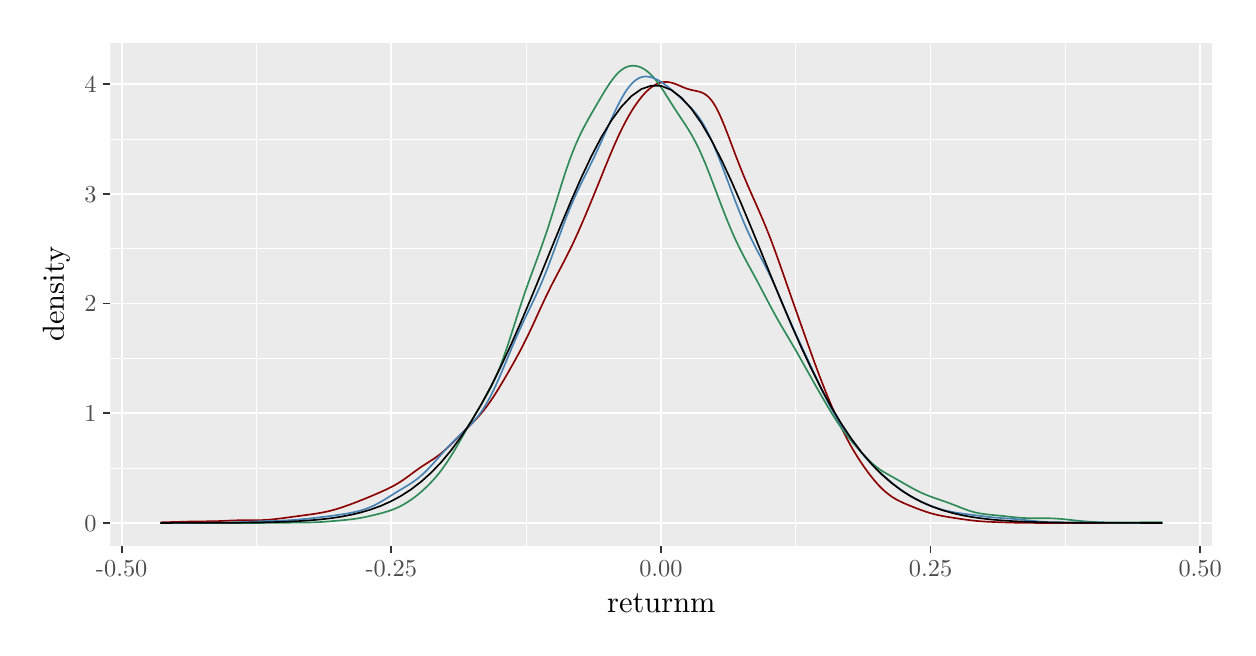
\begin{tikzpicture}[x=1pt,y=1pt]
\definecolor{fillColor}{RGB}{255,255,255}
\path[use as bounding box,fill=fillColor,fill opacity=0.00] (0,0) rectangle (433.62,216.81);
\begin{scope}
\path[clip] (  0.00,  0.00) rectangle (433.62,216.81);
\definecolor{drawColor}{RGB}{255,255,255}
\definecolor{fillColor}{RGB}{255,255,255}

\path[draw=drawColor,line width= 0.6pt,line join=round,line cap=round,fill=fillColor] (  0.00,  0.00) rectangle (433.62,216.81);
\end{scope}
\begin{scope}
\path[clip] ( 29.87, 29.59) rectangle (428.12,211.31);
\definecolor{fillColor}{gray}{0.92}

\path[fill=fillColor] ( 29.87, 29.59) rectangle (428.12,211.31);
\definecolor{drawColor}{RGB}{255,255,255}

\path[draw=drawColor,line width= 0.3pt,line join=round] ( 29.87, 57.67) --
	(428.12, 57.67);

\path[draw=drawColor,line width= 0.3pt,line join=round] ( 29.87, 97.30) --
	(428.12, 97.30);

\path[draw=drawColor,line width= 0.3pt,line join=round] ( 29.87,136.94) --
	(428.12,136.94);

\path[draw=drawColor,line width= 0.3pt,line join=round] ( 29.87,176.58) --
	(428.12,176.58);

\path[draw=drawColor,line width= 0.3pt,line join=round] ( 82.68, 29.59) --
	( 82.68,211.31);

\path[draw=drawColor,line width= 0.3pt,line join=round] (180.11, 29.59) --
	(180.11,211.31);

\path[draw=drawColor,line width= 0.3pt,line join=round] (277.54, 29.59) --
	(277.54,211.31);

\path[draw=drawColor,line width= 0.3pt,line join=round] (374.97, 29.59) --
	(374.97,211.31);

\path[draw=drawColor,line width= 0.6pt,line join=round] ( 29.87, 37.85) --
	(428.12, 37.85);

\path[draw=drawColor,line width= 0.6pt,line join=round] ( 29.87, 77.49) --
	(428.12, 77.49);

\path[draw=drawColor,line width= 0.6pt,line join=round] ( 29.87,117.12) --
	(428.12,117.12);

\path[draw=drawColor,line width= 0.6pt,line join=round] ( 29.87,156.76) --
	(428.12,156.76);

\path[draw=drawColor,line width= 0.6pt,line join=round] ( 29.87,196.40) --
	(428.12,196.40);

\path[draw=drawColor,line width= 0.6pt,line join=round] ( 33.97, 29.59) --
	( 33.97,211.31);

\path[draw=drawColor,line width= 0.6pt,line join=round] (131.40, 29.59) --
	(131.40,211.31);

\path[draw=drawColor,line width= 0.6pt,line join=round] (228.83, 29.59) --
	(228.83,211.31);

\path[draw=drawColor,line width= 0.6pt,line join=round] (326.26, 29.59) --
	(326.26,211.31);

\path[draw=drawColor,line width= 0.6pt,line join=round] (423.69, 29.59) --
	(423.69,211.31);
\definecolor{drawColor}{RGB}{139,0,0}

\path[draw=drawColor,line width= 0.6pt,line join=round] ( 47.97, 38.05) --
	( 48.68, 38.07) --
	( 49.39, 38.09) --
	( 50.10, 38.11) --
	( 50.81, 38.13) --
	( 51.51, 38.15) --
	( 52.22, 38.17) --
	( 52.93, 38.19) --
	( 53.64, 38.21) --
	( 54.35, 38.23) --
	( 55.06, 38.25) --
	( 55.76, 38.27) --
	( 56.47, 38.29) --
	( 57.18, 38.31) --
	( 57.89, 38.33) --
	( 58.60, 38.35) --
	( 59.31, 38.36) --
	( 60.02, 38.37) --
	( 60.72, 38.39) --
	( 61.43, 38.40) --
	( 62.14, 38.40) --
	( 62.85, 38.41) --
	( 63.56, 38.42) --
	( 64.27, 38.42) --
	( 64.98, 38.43) --
	( 65.68, 38.44) --
	( 66.39, 38.45) --
	( 67.10, 38.46) --
	( 67.81, 38.48) --
	( 68.52, 38.50) --
	( 69.23, 38.52) --
	( 69.93, 38.55) --
	( 70.64, 38.58) --
	( 71.35, 38.61) --
	( 72.06, 38.65) --
	( 72.77, 38.68) --
	( 73.48, 38.72) --
	( 74.19, 38.74) --
	( 74.89, 38.77) --
	( 75.60, 38.79) --
	( 76.31, 38.81) --
	( 77.02, 38.82) --
	( 77.73, 38.82) --
	( 78.44, 38.82) --
	( 79.15, 38.82) --
	( 79.85, 38.82) --
	( 80.56, 38.81) --
	( 81.27, 38.81) --
	( 81.98, 38.81) --
	( 82.69, 38.82) --
	( 83.40, 38.83) --
	( 84.10, 38.85) --
	( 84.81, 38.87) --
	( 85.52, 38.91) --
	( 86.23, 38.95) --
	( 86.94, 39.00) --
	( 87.65, 39.06) --
	( 88.36, 39.13) --
	( 89.06, 39.20) --
	( 89.77, 39.28) --
	( 90.48, 39.37) --
	( 91.19, 39.45) --
	( 91.90, 39.54) --
	( 92.61, 39.63) --
	( 93.32, 39.73) --
	( 94.02, 39.82) --
	( 94.73, 39.92) --
	( 95.44, 40.02) --
	( 96.15, 40.11) --
	( 96.86, 40.21) --
	( 97.57, 40.30) --
	( 98.28, 40.40) --
	( 98.98, 40.49) --
	( 99.69, 40.59) --
	(100.40, 40.68) --
	(101.11, 40.78) --
	(101.82, 40.87) --
	(102.53, 40.97) --
	(103.23, 41.07) --
	(103.94, 41.18) --
	(104.65, 41.29) --
	(105.36, 41.41) --
	(106.07, 41.53) --
	(106.78, 41.67) --
	(107.49, 41.81) --
	(108.19, 41.96) --
	(108.90, 42.13) --
	(109.61, 42.31) --
	(110.32, 42.49) --
	(111.03, 42.69) --
	(111.74, 42.90) --
	(112.45, 43.12) --
	(113.15, 43.35) --
	(113.86, 43.58) --
	(114.57, 43.83) --
	(115.28, 44.08) --
	(115.99, 44.33) --
	(116.70, 44.59) --
	(117.40, 44.85) --
	(118.11, 45.12) --
	(118.82, 45.39) --
	(119.53, 45.67) --
	(120.24, 45.95) --
	(120.95, 46.23) --
	(121.66, 46.51) --
	(122.36, 46.80) --
	(123.07, 47.10) --
	(123.78, 47.39) --
	(124.49, 47.69) --
	(125.20, 48.00) --
	(125.91, 48.30) --
	(126.62, 48.61) --
	(127.32, 48.92) --
	(128.03, 49.23) --
	(128.74, 49.55) --
	(129.45, 49.88) --
	(130.16, 50.21) --
	(130.87, 50.56) --
	(131.57, 50.92) --
	(132.28, 51.30) --
	(132.99, 51.69) --
	(133.70, 52.11) --
	(134.41, 52.55) --
	(135.12, 53.01) --
	(135.83, 53.49) --
	(136.53, 53.98) --
	(137.24, 54.49) --
	(137.95, 55.01) --
	(138.66, 55.54) --
	(139.37, 56.06) --
	(140.08, 56.58) --
	(140.79, 57.09) --
	(141.49, 57.59) --
	(142.20, 58.08) --
	(142.91, 58.55) --
	(143.62, 59.02) --
	(144.33, 59.47) --
	(145.04, 59.92) --
	(145.74, 60.38) --
	(146.45, 60.84) --
	(147.16, 61.32) --
	(147.87, 61.83) --
	(148.58, 62.35) --
	(149.29, 62.91) --
	(150.00, 63.49) --
	(150.70, 64.10) --
	(151.41, 64.74) --
	(152.12, 65.40) --
	(152.83, 66.09) --
	(153.54, 66.78) --
	(154.25, 67.49) --
	(154.96, 68.20) --
	(155.66, 68.92) --
	(156.37, 69.63) --
	(157.08, 70.34) --
	(157.79, 71.05) --
	(158.50, 71.76) --
	(159.21, 72.46) --
	(159.92, 73.17) --
	(160.62, 73.89) --
	(161.33, 74.62) --
	(162.04, 75.37) --
	(162.75, 76.14) --
	(163.46, 76.94) --
	(164.17, 77.77) --
	(164.87, 78.64) --
	(165.58, 79.56) --
	(166.29, 80.51) --
	(167.00, 81.51) --
	(167.71, 82.54) --
	(168.42, 83.61) --
	(169.13, 84.72) --
	(169.83, 85.85) --
	(170.54, 87.01) --
	(171.25, 88.20) --
	(171.96, 89.39) --
	(172.67, 90.60) --
	(173.38, 91.82) --
	(174.09, 93.05) --
	(174.79, 94.30) --
	(175.50, 95.55) --
	(176.21, 96.82) --
	(176.92, 98.11) --
	(177.63, 99.43) --
	(178.34,100.77) --
	(179.04,102.15) --
	(179.75,103.55) --
	(180.46,104.99) --
	(181.17,106.46) --
	(181.88,107.96) --
	(182.59,109.48) --
	(183.30,111.02) --
	(184.00,112.57) --
	(184.71,114.12) --
	(185.42,115.66) --
	(186.13,117.19) --
	(186.84,118.70) --
	(187.55,120.18) --
	(188.26,121.63) --
	(188.96,123.06) --
	(189.67,124.46) --
	(190.38,125.83) --
	(191.09,127.18) --
	(191.80,128.53) --
	(192.51,129.87) --
	(193.21,131.22) --
	(193.92,132.57) --
	(194.63,133.95) --
	(195.34,135.36) --
	(196.05,136.79) --
	(196.76,138.26) --
	(197.47,139.77) --
	(198.17,141.31) --
	(198.88,142.88) --
	(199.59,144.49) --
	(200.30,146.11) --
	(201.01,147.77) --
	(201.72,149.44) --
	(202.43,151.13) --
	(203.13,152.83) --
	(203.84,154.54) --
	(204.55,156.27) --
	(205.26,158.01) --
	(205.97,159.75) --
	(206.68,161.50) --
	(207.39,163.25) --
	(208.09,165.00) --
	(208.80,166.75) --
	(209.51,168.48) --
	(210.22,170.20) --
	(210.93,171.89) --
	(211.64,173.54) --
	(212.34,175.16) --
	(213.05,176.74) --
	(213.76,178.27) --
	(214.47,179.75) --
	(215.18,181.18) --
	(215.89,182.55) --
	(216.60,183.86) --
	(217.30,185.11) --
	(218.01,186.31) --
	(218.72,187.45) --
	(219.43,188.54) --
	(220.14,189.57) --
	(220.85,190.54) --
	(221.56,191.45) --
	(222.26,192.30) --
	(222.97,193.09) --
	(223.68,193.80) --
	(224.39,194.46) --
	(225.10,195.05) --
	(225.81,195.57) --
	(226.51,196.02) --
	(227.22,196.40) --
	(227.93,196.70) --
	(228.64,196.94) --
	(229.35,197.10) --
	(230.06,197.18) --
	(230.77,197.19) --
	(231.47,197.14) --
	(232.18,197.02) --
	(232.89,196.84) --
	(233.60,196.62) --
	(234.31,196.36) --
	(235.02,196.07) --
	(235.73,195.76) --
	(236.43,195.46) --
	(237.14,195.17) --
	(237.85,194.90) --
	(238.56,194.66) --
	(239.27,194.45) --
	(239.98,194.27) --
	(240.68,194.12) --
	(241.39,193.97) --
	(242.10,193.82) --
	(242.81,193.64) --
	(243.52,193.40) --
	(244.23,193.08) --
	(244.94,192.65) --
	(245.64,192.11) --
	(246.35,191.43) --
	(247.06,190.59) --
	(247.77,189.60) --
	(248.48,188.46) --
	(249.19,187.14) --
	(249.90,185.69) --
	(250.60,184.12) --
	(251.31,182.44) --
	(252.02,180.68) --
	(252.73,178.86) --
	(253.44,177.00) --
	(254.15,175.12) --
	(254.85,173.23) --
	(255.56,171.35) --
	(256.27,169.49) --
	(256.98,167.66) --
	(257.69,165.87) --
	(258.40,164.11) --
	(259.11,162.39) --
	(259.81,160.71) --
	(260.52,159.06) --
	(261.23,157.44) --
	(261.94,155.84) --
	(262.65,154.24) --
	(263.36,152.65) --
	(264.07,151.05) --
	(264.77,149.42) --
	(265.48,147.78) --
	(266.19,146.09) --
	(266.90,144.37) --
	(267.61,142.60) --
	(268.32,140.79) --
	(269.03,138.92) --
	(269.73,137.02) --
	(270.44,135.08) --
	(271.15,133.10) --
	(271.86,131.10) --
	(272.57,129.09) --
	(273.28,127.06) --
	(273.98,125.03) --
	(274.69,122.99) --
	(275.40,120.96) --
	(276.11,118.93) --
	(276.82,116.91) --
	(277.53,114.90) --
	(278.24,112.89) --
	(278.94,110.89) --
	(279.65,108.88) --
	(280.36,106.88) --
	(281.07,104.88) --
	(281.78,102.89) --
	(282.49,100.91) --
	(283.20, 98.93) --
	(283.90, 96.97) --
	(284.61, 95.03) --
	(285.32, 93.12) --
	(286.03, 91.23) --
	(286.74, 89.37) --
	(287.45, 87.55) --
	(288.15, 85.76) --
	(288.86, 84.02) --
	(289.57, 82.30) --
	(290.28, 80.62) --
	(290.99, 78.97) --
	(291.70, 77.36) --
	(292.41, 75.78) --
	(293.11, 74.24) --
	(293.82, 72.74) --
	(294.53, 71.28) --
	(295.24, 69.86) --
	(295.95, 68.48) --
	(296.66, 67.15) --
	(297.37, 65.86) --
	(298.07, 64.62) --
	(298.78, 63.42) --
	(299.49, 62.26) --
	(300.20, 61.13) --
	(300.91, 60.05) --
	(301.62, 59.00) --
	(302.32, 57.98) --
	(303.03, 56.99) --
	(303.74, 56.02) --
	(304.45, 55.09) --
	(305.16, 54.19) --
	(305.87, 53.32) --
	(306.58, 52.49) --
	(307.28, 51.70) --
	(307.99, 50.95) --
	(308.70, 50.24) --
	(309.41, 49.57) --
	(310.12, 48.96) --
	(310.83, 48.38) --
	(311.54, 47.84) --
	(312.24, 47.35) --
	(312.95, 46.89) --
	(313.66, 46.47) --
	(314.37, 46.08) --
	(315.08, 45.72) --
	(315.79, 45.38) --
	(316.49, 45.05) --
	(317.20, 44.74) --
	(317.91, 44.44) --
	(318.62, 44.15) --
	(319.33, 43.86) --
	(320.04, 43.58) --
	(320.75, 43.30) --
	(321.45, 43.03) --
	(322.16, 42.76) --
	(322.87, 42.50) --
	(323.58, 42.25) --
	(324.29, 42.00) --
	(325.00, 41.77) --
	(325.71, 41.55) --
	(326.41, 41.33) --
	(327.12, 41.14) --
	(327.83, 40.95) --
	(328.54, 40.78) --
	(329.25, 40.63) --
	(329.96, 40.48) --
	(330.67, 40.34) --
	(331.37, 40.21) --
	(332.08, 40.09) --
	(332.79, 39.97) --
	(333.50, 39.85) --
	(334.21, 39.74) --
	(334.92, 39.63) --
	(335.62, 39.53) --
	(336.33, 39.42) --
	(337.04, 39.31) --
	(337.75, 39.21) --
	(338.46, 39.11) --
	(339.17, 39.01) --
	(339.88, 38.92) --
	(340.58, 38.83) --
	(341.29, 38.74) --
	(342.00, 38.66) --
	(342.71, 38.59) --
	(343.42, 38.52) --
	(344.13, 38.46) --
	(344.84, 38.41) --
	(345.54, 38.36) --
	(346.25, 38.32) --
	(346.96, 38.28) --
	(347.67, 38.24) --
	(348.38, 38.21) --
	(349.09, 38.18) --
	(349.79, 38.15) --
	(350.50, 38.13) --
	(351.21, 38.10) --
	(351.92, 38.08) --
	(352.63, 38.05) --
	(353.34, 38.03) --
	(354.05, 38.01) --
	(354.75, 37.99) --
	(355.46, 37.97) --
	(356.17, 37.95) --
	(356.88, 37.93) --
	(357.59, 37.92) --
	(358.30, 37.91) --
	(359.01, 37.89) --
	(359.71, 37.88) --
	(360.42, 37.88) --
	(361.13, 37.87) --
	(361.84, 37.86) --
	(362.55, 37.86) --
	(363.26, 37.86) --
	(363.96, 37.85) --
	(364.67, 37.85) --
	(365.38, 37.85) --
	(366.09, 37.85) --
	(366.80, 37.85) --
	(367.51, 37.85) --
	(368.22, 37.85) --
	(368.92, 37.85) --
	(369.63, 37.85) --
	(370.34, 37.85) --
	(371.05, 37.85) --
	(371.76, 37.85) --
	(372.47, 37.85) --
	(373.18, 37.85) --
	(373.88, 37.85) --
	(374.59, 37.85) --
	(375.30, 37.85) --
	(376.01, 37.85) --
	(376.72, 37.85) --
	(377.43, 37.85) --
	(378.13, 37.85) --
	(378.84, 37.85) --
	(379.55, 37.85) --
	(380.26, 37.85) --
	(380.97, 37.85) --
	(381.68, 37.85) --
	(382.39, 37.85) --
	(383.09, 37.85) --
	(383.80, 37.85) --
	(384.51, 37.85) --
	(385.22, 37.85) --
	(385.93, 37.85) --
	(386.64, 37.85) --
	(387.35, 37.85) --
	(388.05, 37.85) --
	(388.76, 37.85) --
	(389.47, 37.85) --
	(390.18, 37.85) --
	(390.89, 37.85) --
	(391.60, 37.85) --
	(392.31, 37.85) --
	(393.01, 37.85) --
	(393.72, 37.85) --
	(394.43, 37.85) --
	(395.14, 37.85) --
	(395.85, 37.85) --
	(396.56, 37.85) --
	(397.26, 37.85) --
	(397.97, 37.85) --
	(398.68, 37.85) --
	(399.39, 37.85) --
	(400.10, 37.85) --
	(400.81, 37.85) --
	(401.52, 37.85) --
	(402.22, 37.85) --
	(402.93, 37.85) --
	(403.64, 37.85) --
	(404.35, 37.85) --
	(405.06, 37.85) --
	(405.77, 37.85) --
	(406.48, 37.85) --
	(407.18, 37.85) --
	(407.89, 37.85) --
	(408.60, 37.85) --
	(409.31, 37.85) --
	(410.02, 37.85);
\definecolor{drawColor}{RGB}{46,139,87}

\path[draw=drawColor,line width= 0.6pt,line join=round] ( 47.97, 37.85) --
	( 48.68, 37.85) --
	( 49.39, 37.85) --
	( 50.10, 37.85) --
	( 50.81, 37.85) --
	( 51.51, 37.85) --
	( 52.22, 37.85) --
	( 52.93, 37.85) --
	( 53.64, 37.85) --
	( 54.35, 37.85) --
	( 55.06, 37.85) --
	( 55.76, 37.85) --
	( 56.47, 37.85) --
	( 57.18, 37.85) --
	( 57.89, 37.85) --
	( 58.60, 37.85) --
	( 59.31, 37.85) --
	( 60.02, 37.85) --
	( 60.72, 37.85) --
	( 61.43, 37.85) --
	( 62.14, 37.85) --
	( 62.85, 37.85) --
	( 63.56, 37.85) --
	( 64.27, 37.85) --
	( 64.98, 37.85) --
	( 65.68, 37.85) --
	( 66.39, 37.85) --
	( 67.10, 37.85) --
	( 67.81, 37.85) --
	( 68.52, 37.85) --
	( 69.23, 37.85) --
	( 69.93, 37.85) --
	( 70.64, 37.85) --
	( 71.35, 37.85) --
	( 72.06, 37.85) --
	( 72.77, 37.85) --
	( 73.48, 37.85) --
	( 74.19, 37.85) --
	( 74.89, 37.85) --
	( 75.60, 37.85) --
	( 76.31, 37.85) --
	( 77.02, 37.85) --
	( 77.73, 37.85) --
	( 78.44, 37.85) --
	( 79.15, 37.85) --
	( 79.85, 37.85) --
	( 80.56, 37.85) --
	( 81.27, 37.85) --
	( 81.98, 37.85) --
	( 82.69, 37.85) --
	( 83.40, 37.85) --
	( 84.10, 37.85) --
	( 84.81, 37.85) --
	( 85.52, 37.85) --
	( 86.23, 37.86) --
	( 86.94, 37.86) --
	( 87.65, 37.87) --
	( 88.36, 37.87) --
	( 89.06, 37.88) --
	( 89.77, 37.88) --
	( 90.48, 37.89) --
	( 91.19, 37.90) --
	( 91.90, 37.91) --
	( 92.61, 37.92) --
	( 93.32, 37.92) --
	( 94.02, 37.93) --
	( 94.73, 37.94) --
	( 95.44, 37.95) --
	( 96.15, 37.96) --
	( 96.86, 37.97) --
	( 97.57, 37.97) --
	( 98.28, 37.98) --
	( 98.98, 37.99) --
	( 99.69, 37.99) --
	(100.40, 38.00) --
	(101.11, 38.01) --
	(101.82, 38.02) --
	(102.53, 38.04) --
	(103.23, 38.06) --
	(103.94, 38.08) --
	(104.65, 38.11) --
	(105.36, 38.15) --
	(106.07, 38.19) --
	(106.78, 38.23) --
	(107.49, 38.28) --
	(108.19, 38.34) --
	(108.90, 38.40) --
	(109.61, 38.46) --
	(110.32, 38.52) --
	(111.03, 38.58) --
	(111.74, 38.65) --
	(112.45, 38.71) --
	(113.15, 38.77) --
	(113.86, 38.84) --
	(114.57, 38.90) --
	(115.28, 38.97) --
	(115.99, 39.05) --
	(116.70, 39.13) --
	(117.40, 39.21) --
	(118.11, 39.31) --
	(118.82, 39.41) --
	(119.53, 39.53) --
	(120.24, 39.65) --
	(120.95, 39.78) --
	(121.66, 39.92) --
	(122.36, 40.07) --
	(123.07, 40.23) --
	(123.78, 40.39) --
	(124.49, 40.55) --
	(125.20, 40.72) --
	(125.91, 40.89) --
	(126.62, 41.07) --
	(127.32, 41.25) --
	(128.03, 41.44) --
	(128.74, 41.64) --
	(129.45, 41.84) --
	(130.16, 42.06) --
	(130.87, 42.30) --
	(131.57, 42.55) --
	(132.28, 42.82) --
	(132.99, 43.11) --
	(133.70, 43.42) --
	(134.41, 43.76) --
	(135.12, 44.12) --
	(135.83, 44.51) --
	(136.53, 44.92) --
	(137.24, 45.36) --
	(137.95, 45.82) --
	(138.66, 46.31) --
	(139.37, 46.82) --
	(140.08, 47.35) --
	(140.79, 47.91) --
	(141.49, 48.49) --
	(142.20, 49.10) --
	(142.91, 49.72) --
	(143.62, 50.38) --
	(144.33, 51.06) --
	(145.04, 51.76) --
	(145.74, 52.50) --
	(146.45, 53.26) --
	(147.16, 54.05) --
	(147.87, 54.89) --
	(148.58, 55.75) --
	(149.29, 56.66) --
	(150.00, 57.60) --
	(150.70, 58.60) --
	(151.41, 59.63) --
	(152.12, 60.70) --
	(152.83, 61.81) --
	(153.54, 62.95) --
	(154.25, 64.12) --
	(154.96, 65.32) --
	(155.66, 66.54) --
	(156.37, 67.77) --
	(157.08, 69.01) --
	(157.79, 70.26) --
	(158.50, 71.50) --
	(159.21, 72.73) --
	(159.92, 73.96) --
	(160.62, 75.17) --
	(161.33, 76.38) --
	(162.04, 77.57) --
	(162.75, 78.75) --
	(163.46, 79.93) --
	(164.17, 81.11) --
	(164.87, 82.31) --
	(165.58, 83.54) --
	(166.29, 84.81) --
	(167.00, 86.14) --
	(167.71, 87.52) --
	(168.42, 88.99) --
	(169.13, 90.53) --
	(169.83, 92.18) --
	(170.54, 93.93) --
	(171.25, 95.77) --
	(171.96, 97.70) --
	(172.67, 99.72) --
	(173.38,101.80) --
	(174.09,103.94) --
	(174.79,106.13) --
	(175.50,108.34) --
	(176.21,110.56) --
	(176.92,112.77) --
	(177.63,114.96) --
	(178.34,117.11) --
	(179.04,119.23) --
	(179.75,121.30) --
	(180.46,123.33) --
	(181.17,125.32) --
	(181.88,127.28) --
	(182.59,129.21) --
	(183.30,131.13) --
	(184.00,133.05) --
	(184.71,134.99) --
	(185.42,136.96) --
	(186.13,138.97) --
	(186.84,141.02) --
	(187.55,143.12) --
	(188.26,145.28) --
	(188.96,147.48) --
	(189.67,149.73) --
	(190.38,152.02) --
	(191.09,154.32) --
	(191.80,156.62) --
	(192.51,158.90) --
	(193.21,161.16) --
	(193.92,163.36) --
	(194.63,165.51) --
	(195.34,167.57) --
	(196.05,169.56) --
	(196.76,171.43) --
	(197.47,173.22) --
	(198.17,174.90) --
	(198.88,176.50) --
	(199.59,178.02) --
	(200.30,179.47) --
	(201.01,180.85) --
	(201.72,182.17) --
	(202.43,183.46) --
	(203.13,184.72) --
	(203.84,185.96) --
	(204.55,187.18) --
	(205.26,188.40) --
	(205.97,189.62) --
	(206.68,190.83) --
	(207.39,192.02) --
	(208.09,193.20) --
	(208.80,194.36) --
	(209.51,195.48) --
	(210.22,196.55) --
	(210.93,197.56) --
	(211.64,198.51) --
	(212.34,199.37) --
	(213.05,200.16) --
	(213.76,200.85) --
	(214.47,201.45) --
	(215.18,201.96) --
	(215.89,202.36) --
	(216.60,202.67) --
	(217.30,202.88) --
	(218.01,203.01) --
	(218.72,203.05) --
	(219.43,203.01) --
	(220.14,202.90) --
	(220.85,202.71) --
	(221.56,202.45) --
	(222.26,202.11) --
	(222.97,201.69) --
	(223.68,201.19) --
	(224.39,200.61) --
	(225.10,199.95) --
	(225.81,199.22) --
	(226.51,198.42) --
	(227.22,197.54) --
	(227.93,196.60) --
	(228.64,195.60) --
	(229.35,194.55) --
	(230.06,193.46) --
	(230.77,192.35) --
	(231.47,191.23) --
	(232.18,190.10) --
	(232.89,188.98) --
	(233.60,187.87) --
	(234.31,186.77) --
	(235.02,185.70) --
	(235.73,184.63) --
	(236.43,183.57) --
	(237.14,182.50) --
	(237.85,181.42) --
	(238.56,180.31) --
	(239.27,179.15) --
	(239.98,177.95) --
	(240.68,176.68) --
	(241.39,175.35) --
	(242.10,173.93) --
	(242.81,172.44) --
	(243.52,170.86) --
	(244.23,169.22) --
	(244.94,167.52) --
	(245.64,165.76) --
	(246.35,163.95) --
	(247.06,162.11) --
	(247.77,160.25) --
	(248.48,158.36) --
	(249.19,156.48) --
	(249.90,154.60) --
	(250.60,152.73) --
	(251.31,150.89) --
	(252.02,149.08) --
	(252.73,147.30) --
	(253.44,145.57) --
	(254.15,143.88) --
	(254.85,142.25) --
	(255.56,140.68) --
	(256.27,139.16) --
	(256.98,137.69) --
	(257.69,136.27) --
	(258.40,134.89) --
	(259.11,133.54) --
	(259.81,132.21) --
	(260.52,130.91) --
	(261.23,129.61) --
	(261.94,128.31) --
	(262.65,127.01) --
	(263.36,125.69) --
	(264.07,124.37) --
	(264.77,123.03) --
	(265.48,121.68) --
	(266.19,120.33) --
	(266.90,118.98) --
	(267.61,117.63) --
	(268.32,116.29) --
	(269.03,114.97) --
	(269.73,113.67) --
	(270.44,112.39) --
	(271.15,111.13) --
	(271.86,109.89) --
	(272.57,108.67) --
	(273.28,107.47) --
	(273.98,106.27) --
	(274.69,105.08) --
	(275.40,103.88) --
	(276.11,102.68) --
	(276.82,101.47) --
	(277.53,100.25) --
	(278.24, 99.01) --
	(278.94, 97.76) --
	(279.65, 96.51) --
	(280.36, 95.24) --
	(281.07, 93.97) --
	(281.78, 92.70) --
	(282.49, 91.44) --
	(283.20, 90.17) --
	(283.90, 88.91) --
	(284.61, 87.66) --
	(285.32, 86.41) --
	(286.03, 85.17) --
	(286.74, 83.94) --
	(287.45, 82.71) --
	(288.15, 81.50) --
	(288.86, 80.30) --
	(289.57, 79.11) --
	(290.28, 77.94) --
	(290.99, 76.79) --
	(291.70, 75.67) --
	(292.41, 74.58) --
	(293.11, 73.52) --
	(293.82, 72.49) --
	(294.53, 71.49) --
	(295.24, 70.53) --
	(295.95, 69.60) --
	(296.66, 68.69) --
	(297.37, 67.81) --
	(298.07, 66.96) --
	(298.78, 66.12) --
	(299.49, 65.29) --
	(300.20, 64.48) --
	(300.91, 63.69) --
	(301.62, 62.91) --
	(302.32, 62.15) --
	(303.03, 61.42) --
	(303.74, 60.71) --
	(304.45, 60.03) --
	(305.16, 59.38) --
	(305.87, 58.77) --
	(306.58, 58.19) --
	(307.28, 57.66) --
	(307.99, 57.15) --
	(308.70, 56.68) --
	(309.41, 56.24) --
	(310.12, 55.81) --
	(310.83, 55.41) --
	(311.54, 55.01) --
	(312.24, 54.61) --
	(312.95, 54.22) --
	(313.66, 53.82) --
	(314.37, 53.42) --
	(315.08, 53.02) --
	(315.79, 52.61) --
	(316.49, 52.20) --
	(317.20, 51.79) --
	(317.91, 51.38) --
	(318.62, 50.98) --
	(319.33, 50.58) --
	(320.04, 50.20) --
	(320.75, 49.82) --
	(321.45, 49.46) --
	(322.16, 49.11) --
	(322.87, 48.78) --
	(323.58, 48.46) --
	(324.29, 48.16) --
	(325.00, 47.87) --
	(325.71, 47.59) --
	(326.41, 47.32) --
	(327.12, 47.06) --
	(327.83, 46.81) --
	(328.54, 46.56) --
	(329.25, 46.32) --
	(329.96, 46.08) --
	(330.67, 45.83) --
	(331.37, 45.59) --
	(332.08, 45.34) --
	(332.79, 45.08) --
	(333.50, 44.82) --
	(334.21, 44.55) --
	(334.92, 44.27) --
	(335.62, 43.99) --
	(336.33, 43.71) --
	(337.04, 43.43) --
	(337.75, 43.16) --
	(338.46, 42.89) --
	(339.17, 42.63) --
	(339.88, 42.38) --
	(340.58, 42.15) --
	(341.29, 41.94) --
	(342.00, 41.75) --
	(342.71, 41.58) --
	(343.42, 41.43) --
	(344.13, 41.29) --
	(344.84, 41.17) --
	(345.54, 41.07) --
	(346.25, 40.98) --
	(346.96, 40.90) --
	(347.67, 40.82) --
	(348.38, 40.75) --
	(349.09, 40.69) --
	(349.79, 40.62) --
	(350.50, 40.55) --
	(351.21, 40.48) --
	(351.92, 40.41) --
	(352.63, 40.34) --
	(353.34, 40.26) --
	(354.05, 40.18) --
	(354.75, 40.10) --
	(355.46, 40.02) --
	(356.17, 39.94) --
	(356.88, 39.87) --
	(357.59, 39.80) --
	(358.30, 39.74) --
	(359.01, 39.69) --
	(359.71, 39.64) --
	(360.42, 39.61) --
	(361.13, 39.58) --
	(361.84, 39.56) --
	(362.55, 39.55) --
	(363.26, 39.54) --
	(363.96, 39.54) --
	(364.67, 39.54) --
	(365.38, 39.54) --
	(366.09, 39.55) --
	(366.80, 39.55) --
	(367.51, 39.55) --
	(368.22, 39.54) --
	(368.92, 39.53) --
	(369.63, 39.51) --
	(370.34, 39.49) --
	(371.05, 39.45) --
	(371.76, 39.41) --
	(372.47, 39.36) --
	(373.18, 39.31) --
	(373.88, 39.25) --
	(374.59, 39.18) --
	(375.30, 39.10) --
	(376.01, 39.03) --
	(376.72, 38.95) --
	(377.43, 38.87) --
	(378.13, 38.79) --
	(378.84, 38.71) --
	(379.55, 38.64) --
	(380.26, 38.57) --
	(380.97, 38.50) --
	(381.68, 38.44) --
	(382.39, 38.38) --
	(383.09, 38.33) --
	(383.80, 38.28) --
	(384.51, 38.24) --
	(385.22, 38.20) --
	(385.93, 38.17) --
	(386.64, 38.14) --
	(387.35, 38.11) --
	(388.05, 38.09) --
	(388.76, 38.07) --
	(389.47, 38.05) --
	(390.18, 38.04) --
	(390.89, 38.02) --
	(391.60, 38.01) --
	(392.31, 38.01) --
	(393.01, 38.00) --
	(393.72, 38.00) --
	(394.43, 38.00) --
	(395.14, 38.00) --
	(395.85, 38.00) --
	(396.56, 38.01) --
	(397.26, 38.01) --
	(397.97, 38.02) --
	(398.68, 38.03) --
	(399.39, 38.04) --
	(400.10, 38.05) --
	(400.81, 38.05) --
	(401.52, 38.06) --
	(402.22, 38.07) --
	(402.93, 38.08) --
	(403.64, 38.09) --
	(404.35, 38.09) --
	(405.06, 38.10) --
	(405.77, 38.10) --
	(406.48, 38.10) --
	(407.18, 38.10) --
	(407.89, 38.09) --
	(408.60, 38.09) --
	(409.31, 38.08) --
	(410.02, 38.07);
\definecolor{drawColor}{RGB}{70,130,180}

\path[draw=drawColor,line width= 0.6pt,line join=round] ( 47.97, 37.85) --
	( 48.68, 37.85) --
	( 49.39, 37.85) --
	( 50.10, 37.85) --
	( 50.81, 37.85) --
	( 51.51, 37.85) --
	( 52.22, 37.85) --
	( 52.93, 37.85) --
	( 53.64, 37.85) --
	( 54.35, 37.85) --
	( 55.06, 37.85) --
	( 55.76, 37.85) --
	( 56.47, 37.85) --
	( 57.18, 37.85) --
	( 57.89, 37.85) --
	( 58.60, 37.85) --
	( 59.31, 37.85) --
	( 60.02, 37.86) --
	( 60.72, 37.86) --
	( 61.43, 37.86) --
	( 62.14, 37.87) --
	( 62.85, 37.87) --
	( 63.56, 37.88) --
	( 64.27, 37.89) --
	( 64.98, 37.90) --
	( 65.68, 37.91) --
	( 66.39, 37.92) --
	( 67.10, 37.93) --
	( 67.81, 37.94) --
	( 68.52, 37.95) --
	( 69.23, 37.96) --
	( 69.93, 37.97) --
	( 70.64, 37.99) --
	( 71.35, 38.00) --
	( 72.06, 38.01) --
	( 72.77, 38.03) --
	( 73.48, 38.04) --
	( 74.19, 38.06) --
	( 74.89, 38.08) --
	( 75.60, 38.10) --
	( 76.31, 38.12) --
	( 77.02, 38.15) --
	( 77.73, 38.18) --
	( 78.44, 38.21) --
	( 79.15, 38.24) --
	( 79.85, 38.27) --
	( 80.56, 38.31) --
	( 81.27, 38.34) --
	( 81.98, 38.37) --
	( 82.69, 38.40) --
	( 83.40, 38.43) --
	( 84.10, 38.46) --
	( 84.81, 38.49) --
	( 85.52, 38.51) --
	( 86.23, 38.53) --
	( 86.94, 38.55) --
	( 87.65, 38.57) --
	( 88.36, 38.58) --
	( 89.06, 38.60) --
	( 89.77, 38.62) --
	( 90.48, 38.64) --
	( 91.19, 38.66) --
	( 91.90, 38.69) --
	( 92.61, 38.72) --
	( 93.32, 38.75) --
	( 94.02, 38.79) --
	( 94.73, 38.83) --
	( 95.44, 38.88) --
	( 96.15, 38.93) --
	( 96.86, 38.99) --
	( 97.57, 39.04) --
	( 98.28, 39.11) --
	( 98.98, 39.17) --
	( 99.69, 39.24) --
	(100.40, 39.31) --
	(101.11, 39.38) --
	(101.82, 39.45) --
	(102.53, 39.53) --
	(103.23, 39.61) --
	(103.94, 39.69) --
	(104.65, 39.77) --
	(105.36, 39.85) --
	(106.07, 39.94) --
	(106.78, 40.03) --
	(107.49, 40.11) --
	(108.19, 40.20) --
	(108.90, 40.30) --
	(109.61, 40.39) --
	(110.32, 40.48) --
	(111.03, 40.58) --
	(111.74, 40.68) --
	(112.45, 40.78) --
	(113.15, 40.88) --
	(113.86, 40.99) --
	(114.57, 41.10) --
	(115.28, 41.22) --
	(115.99, 41.35) --
	(116.70, 41.49) --
	(117.40, 41.63) --
	(118.11, 41.78) --
	(118.82, 41.95) --
	(119.53, 42.13) --
	(120.24, 42.32) --
	(120.95, 42.53) --
	(121.66, 42.76) --
	(122.36, 43.00) --
	(123.07, 43.27) --
	(123.78, 43.55) --
	(124.49, 43.86) --
	(125.20, 44.19) --
	(125.91, 44.55) --
	(126.62, 44.92) --
	(127.32, 45.31) --
	(128.03, 45.72) --
	(128.74, 46.15) --
	(129.45, 46.58) --
	(130.16, 47.02) --
	(130.87, 47.46) --
	(131.57, 47.91) --
	(132.28, 48.35) --
	(132.99, 48.79) --
	(133.70, 49.22) --
	(134.41, 49.65) --
	(135.12, 50.07) --
	(135.83, 50.50) --
	(136.53, 50.93) --
	(137.24, 51.36) --
	(137.95, 51.80) --
	(138.66, 52.26) --
	(139.37, 52.74) --
	(140.08, 53.25) --
	(140.79, 53.78) --
	(141.49, 54.35) --
	(142.20, 54.95) --
	(142.91, 55.59) --
	(143.62, 56.26) --
	(144.33, 56.96) --
	(145.04, 57.70) --
	(145.74, 58.46) --
	(146.45, 59.23) --
	(147.16, 60.02) --
	(147.87, 60.82) --
	(148.58, 61.62) --
	(149.29, 62.42) --
	(150.00, 63.21) --
	(150.70, 64.00) --
	(151.41, 64.76) --
	(152.12, 65.52) --
	(152.83, 66.26) --
	(153.54, 66.98) --
	(154.25, 67.69) --
	(154.96, 68.39) --
	(155.66, 69.08) --
	(156.37, 69.76) --
	(157.08, 70.44) --
	(157.79, 71.12) --
	(158.50, 71.81) --
	(159.21, 72.51) --
	(159.92, 73.23) --
	(160.62, 73.97) --
	(161.33, 74.75) --
	(162.04, 75.58) --
	(162.75, 76.46) --
	(163.46, 77.39) --
	(164.17, 78.40) --
	(164.87, 79.48) --
	(165.58, 80.64) --
	(166.29, 81.87) --
	(167.00, 83.17) --
	(167.71, 84.55) --
	(168.42, 85.99) --
	(169.13, 87.50) --
	(169.83, 89.06) --
	(170.54, 90.67) --
	(171.25, 92.32) --
	(171.96, 94.00) --
	(172.67, 95.69) --
	(173.38, 97.39) --
	(174.09, 99.09) --
	(174.79,100.79) --
	(175.50,102.46) --
	(176.21,104.11) --
	(176.92,105.74) --
	(177.63,107.32) --
	(178.34,108.88) --
	(179.04,110.41) --
	(179.75,111.91) --
	(180.46,113.39) --
	(181.17,114.86) --
	(181.88,116.33) --
	(182.59,117.81) --
	(183.30,119.30) --
	(184.00,120.83) --
	(184.71,122.40) --
	(185.42,124.02) --
	(186.13,125.69) --
	(186.84,127.41) --
	(187.55,129.19) --
	(188.26,131.02) --
	(188.96,132.90) --
	(189.67,134.81) --
	(190.38,136.76) --
	(191.09,138.71) --
	(191.80,140.67) --
	(192.51,142.61) --
	(193.21,144.53) --
	(193.92,146.42) --
	(194.63,148.26) --
	(195.34,150.06) --
	(196.05,151.79) --
	(196.76,153.47) --
	(197.47,155.10) --
	(198.17,156.66) --
	(198.88,158.19) --
	(199.59,159.67) --
	(200.30,161.13) --
	(201.01,162.56) --
	(201.72,163.98) --
	(202.43,165.40) --
	(203.13,166.83) --
	(203.84,168.27) --
	(204.55,169.74) --
	(205.26,171.23) --
	(205.97,172.75) --
	(206.68,174.29) --
	(207.39,175.85) --
	(208.09,177.44) --
	(208.80,179.03) --
	(209.51,180.62) --
	(210.22,182.21) --
	(210.93,183.78) --
	(211.64,185.33) --
	(212.34,186.83) --
	(213.05,188.28) --
	(213.76,189.68) --
	(214.47,191.01) --
	(215.18,192.26) --
	(215.89,193.43) --
	(216.60,194.48) --
	(217.30,195.44) --
	(218.01,196.29) --
	(218.72,197.02) --
	(219.43,197.65) --
	(220.14,198.16) --
	(220.85,198.56) --
	(221.56,198.86) --
	(222.26,199.05) --
	(222.97,199.14) --
	(223.68,199.14) --
	(224.39,199.07) --
	(225.10,198.92) --
	(225.81,198.71) --
	(226.51,198.44) --
	(227.22,198.12) --
	(227.93,197.76) --
	(228.64,197.35) --
	(229.35,196.89) --
	(230.06,196.40) --
	(230.77,195.88) --
	(231.47,195.32) --
	(232.18,194.75) --
	(232.89,194.15) --
	(233.60,193.53) --
	(234.31,192.90) --
	(235.02,192.27) --
	(235.73,191.62) --
	(236.43,190.98) --
	(237.14,190.32) --
	(237.85,189.66) --
	(238.56,188.98) --
	(239.27,188.28) --
	(239.98,187.54) --
	(240.68,186.76) --
	(241.39,185.93) --
	(242.10,185.02) --
	(242.81,184.03) --
	(243.52,182.96) --
	(244.23,181.79) --
	(244.94,180.53) --
	(245.64,179.17) --
	(246.35,177.73) --
	(247.06,176.21) --
	(247.77,174.61) --
	(248.48,172.94) --
	(249.19,171.21) --
	(249.90,169.43) --
	(250.60,167.62) --
	(251.31,165.77) --
	(252.02,163.91) --
	(252.73,162.02) --
	(253.44,160.13) --
	(254.15,158.24) --
	(254.85,156.36) --
	(255.56,154.50) --
	(256.27,152.66) --
	(256.98,150.85) --
	(257.69,149.08) --
	(258.40,147.36) --
	(259.11,145.69) --
	(259.81,144.08) --
	(260.52,142.52) --
	(261.23,141.01) --
	(261.94,139.55) --
	(262.65,138.14) --
	(263.36,136.76) --
	(264.07,135.41) --
	(264.77,134.06) --
	(265.48,132.71) --
	(266.19,131.35) --
	(266.90,129.96) --
	(267.61,128.55) --
	(268.32,127.09) --
	(269.03,125.60) --
	(269.73,124.06) --
	(270.44,122.49) --
	(271.15,120.88) --
	(271.86,119.25) --
	(272.57,117.60) --
	(273.28,115.94) --
	(273.98,114.28) --
	(274.69,112.63) --
	(275.40,111.00) --
	(276.11,109.39) --
	(276.82,107.80) --
	(277.53,106.24) --
	(278.24,104.69) --
	(278.94,103.17) --
	(279.65,101.65) --
	(280.36,100.14) --
	(281.07, 98.64) --
	(281.78, 97.12) --
	(282.49, 95.60) --
	(283.20, 94.08) --
	(283.90, 92.54) --
	(284.61, 91.01) --
	(285.32, 89.47) --
	(286.03, 87.95) --
	(286.74, 86.44) --
	(287.45, 84.96) --
	(288.15, 83.51) --
	(288.86, 82.10) --
	(289.57, 80.74) --
	(290.28, 79.43) --
	(290.99, 78.16) --
	(291.70, 76.94) --
	(292.41, 75.77) --
	(293.11, 74.64) --
	(293.82, 73.54) --
	(294.53, 72.48) --
	(295.24, 71.44) --
	(295.95, 70.43) --
	(296.66, 69.43) --
	(297.37, 68.45) --
	(298.07, 67.48) --
	(298.78, 66.53) --
	(299.49, 65.59) --
	(300.20, 64.66) --
	(300.91, 63.76) --
	(301.62, 62.88) --
	(302.32, 62.02) --
	(303.03, 61.19) --
	(303.74, 60.39) --
	(304.45, 59.61) --
	(305.16, 58.86) --
	(305.87, 58.14) --
	(306.58, 57.44) --
	(307.28, 56.76) --
	(307.99, 56.10) --
	(308.70, 55.45) --
	(309.41, 54.82) --
	(310.12, 54.20) --
	(310.83, 53.59) --
	(311.54, 52.99) --
	(312.24, 52.39) --
	(312.95, 51.82) --
	(313.66, 51.25) --
	(314.37, 50.70) --
	(315.08, 50.18) --
	(315.79, 49.67) --
	(316.49, 49.18) --
	(317.20, 48.70) --
	(317.91, 48.25) --
	(318.62, 47.82) --
	(319.33, 47.41) --
	(320.04, 47.01) --
	(320.75, 46.62) --
	(321.45, 46.26) --
	(322.16, 45.90) --
	(322.87, 45.56) --
	(323.58, 45.23) --
	(324.29, 44.91) --
	(325.00, 44.60) --
	(325.71, 44.30) --
	(326.41, 44.02) --
	(327.12, 43.74) --
	(327.83, 43.49) --
	(328.54, 43.24) --
	(329.25, 43.01) --
	(329.96, 42.79) --
	(330.67, 42.59) --
	(331.37, 42.40) --
	(332.08, 42.23) --
	(332.79, 42.07) --
	(333.50, 41.92) --
	(334.21, 41.78) --
	(334.92, 41.65) --
	(335.62, 41.54) --
	(336.33, 41.43) --
	(337.04, 41.32) --
	(337.75, 41.22) --
	(338.46, 41.13) --
	(339.17, 41.04) --
	(339.88, 40.95) --
	(340.58, 40.86) --
	(341.29, 40.77) --
	(342.00, 40.67) --
	(342.71, 40.58) --
	(343.42, 40.49) --
	(344.13, 40.40) --
	(344.84, 40.31) --
	(345.54, 40.22) --
	(346.25, 40.13) --
	(346.96, 40.05) --
	(347.67, 39.98) --
	(348.38, 39.90) --
	(349.09, 39.83) --
	(349.79, 39.77) --
	(350.50, 39.71) --
	(351.21, 39.66) --
	(351.92, 39.61) --
	(352.63, 39.56) --
	(353.34, 39.51) --
	(354.05, 39.46) --
	(354.75, 39.42) --
	(355.46, 39.36) --
	(356.17, 39.31) --
	(356.88, 39.25) --
	(357.59, 39.18) --
	(358.30, 39.12) --
	(359.01, 39.05) --
	(359.71, 38.97) --
	(360.42, 38.89) --
	(361.13, 38.81) --
	(361.84, 38.73) --
	(362.55, 38.66) --
	(363.26, 38.58) --
	(363.96, 38.51) --
	(364.67, 38.44) --
	(365.38, 38.37) --
	(366.09, 38.32) --
	(366.80, 38.27) --
	(367.51, 38.22) --
	(368.22, 38.18) --
	(368.92, 38.15) --
	(369.63, 38.13) --
	(370.34, 38.10) --
	(371.05, 38.09) --
	(371.76, 38.07) --
	(372.47, 38.07) --
	(373.18, 38.06) --
	(373.88, 38.06) --
	(374.59, 38.05) --
	(375.30, 38.05) --
	(376.01, 38.05) --
	(376.72, 38.06) --
	(377.43, 38.06) --
	(378.13, 38.06) --
	(378.84, 38.06) --
	(379.55, 38.07) --
	(380.26, 38.07) --
	(380.97, 38.07) --
	(381.68, 38.07) --
	(382.39, 38.07) --
	(383.09, 38.06) --
	(383.80, 38.06) --
	(384.51, 38.05) --
	(385.22, 38.04) --
	(385.93, 38.03) --
	(386.64, 38.02) --
	(387.35, 38.01) --
	(388.05, 38.00) --
	(388.76, 37.98) --
	(389.47, 37.97) --
	(390.18, 37.95) --
	(390.89, 37.94) --
	(391.60, 37.93) --
	(392.31, 37.92) --
	(393.01, 37.90) --
	(393.72, 37.89) --
	(394.43, 37.89) --
	(395.14, 37.88) --
	(395.85, 37.87) --
	(396.56, 37.87) --
	(397.26, 37.86) --
	(397.97, 37.86) --
	(398.68, 37.86) --
	(399.39, 37.85) --
	(400.10, 37.85) --
	(400.81, 37.85) --
	(401.52, 37.85) --
	(402.22, 37.85) --
	(402.93, 37.85) --
	(403.64, 37.85) --
	(404.35, 37.85) --
	(405.06, 37.85) --
	(405.77, 37.85) --
	(406.48, 37.85) --
	(407.18, 37.85) --
	(407.89, 37.85) --
	(408.60, 37.85) --
	(409.31, 37.85) --
	(410.02, 37.85);
\definecolor{drawColor}{RGB}{0,0,0}

\path[draw=drawColor,line width= 0.6pt,line join=round] ( 47.97, 37.85) --
	( 51.59, 37.85) --
	( 55.21, 37.86) --
	( 58.83, 37.86) --
	( 62.45, 37.87) --
	( 66.07, 37.88) --
	( 69.69, 37.89) --
	( 73.31, 37.91) --
	( 76.93, 37.94) --
	( 80.56, 37.98) --
	( 84.18, 38.04) --
	( 87.80, 38.12) --
	( 91.42, 38.22) --
	( 95.04, 38.36) --
	( 98.66, 38.55) --
	(102.28, 38.80) --
	(105.90, 39.12) --
	(109.52, 39.54) --
	(113.14, 40.08) --
	(116.76, 40.77) --
	(120.38, 41.63) --
	(124.00, 42.70) --
	(127.62, 44.02) --
	(131.24, 45.63) --
	(134.86, 47.59) --
	(138.48, 49.92) --
	(142.10, 52.69) --
	(145.72, 55.94) --
	(149.34, 59.70) --
	(152.96, 64.03) --
	(156.59, 68.94) --
	(160.21, 74.45) --
	(163.83, 80.57) --
	(167.45, 87.28) --
	(171.07, 94.56) --
	(174.69,102.35) --
	(178.31,110.59) --
	(181.93,119.16) --
	(185.55,127.97) --
	(189.17,136.87) --
	(192.79,145.72) --
	(196.41,154.34) --
	(200.03,162.58) --
	(203.65,170.25) --
	(207.27,177.19) --
	(210.89,183.22) --
	(214.51,188.22) --
	(218.13,192.05) --
	(221.75,194.62) --
	(225.37,195.86) --
	(228.99,195.75) --
	(232.61,194.28) --
	(236.24,191.49) --
	(239.86,187.45) --
	(243.48,182.27) --
	(247.10,176.07) --
	(250.72,169.00) --
	(254.34,161.22) --
	(257.96,152.90) --
	(261.58,144.23) --
	(265.20,135.36) --
	(268.82,126.46) --
	(272.44,117.69) --
	(276.06,109.16) --
	(279.68,101.00) --
	(283.30, 93.29) --
	(286.92, 86.10) --
	(290.54, 79.49) --
	(294.16, 73.47) --
	(297.78, 68.06) --
	(301.40, 63.25) --
	(305.02, 59.03) --
	(308.64, 55.35) --
	(312.27, 52.19) --
	(315.89, 49.50) --
	(319.51, 47.23) --
	(323.13, 45.34) --
	(326.75, 43.78) --
	(330.37, 42.50) --
	(333.99, 41.47) --
	(337.61, 40.64) --
	(341.23, 39.98) --
	(344.85, 39.47) --
	(348.47, 39.06) --
	(352.09, 38.75) --
	(355.71, 38.52) --
	(359.33, 38.34) --
	(362.95, 38.20) --
	(366.57, 38.10) --
	(370.19, 38.03) --
	(373.81, 37.98) --
	(377.43, 37.94) --
	(381.05, 37.91) --
	(384.67, 37.89) --
	(388.29, 37.88) --
	(391.92, 37.87) --
	(395.54, 37.86) --
	(399.16, 37.86) --
	(402.78, 37.85) --
	(406.40, 37.85) --
	(410.02, 37.85);
\end{scope}
\begin{scope}
\path[clip] (  0.00,  0.00) rectangle (433.62,216.81);
\definecolor{drawColor}{gray}{0.30}

\node[text=drawColor,anchor=base east,inner sep=0pt, outer sep=0pt, scale=  0.88] at ( 24.92, 34.82) {0};

\node[text=drawColor,anchor=base east,inner sep=0pt, outer sep=0pt, scale=  0.88] at ( 24.92, 74.45) {1};

\node[text=drawColor,anchor=base east,inner sep=0pt, outer sep=0pt, scale=  0.88] at ( 24.92,114.09) {2};

\node[text=drawColor,anchor=base east,inner sep=0pt, outer sep=0pt, scale=  0.88] at ( 24.92,153.73) {3};

\node[text=drawColor,anchor=base east,inner sep=0pt, outer sep=0pt, scale=  0.88] at ( 24.92,193.37) {4};
\end{scope}
\begin{scope}
\path[clip] (  0.00,  0.00) rectangle (433.62,216.81);
\definecolor{drawColor}{gray}{0.20}

\path[draw=drawColor,line width= 0.6pt,line join=round] ( 27.12, 37.85) --
	( 29.87, 37.85);

\path[draw=drawColor,line width= 0.6pt,line join=round] ( 27.12, 77.49) --
	( 29.87, 77.49);

\path[draw=drawColor,line width= 0.6pt,line join=round] ( 27.12,117.12) --
	( 29.87,117.12);

\path[draw=drawColor,line width= 0.6pt,line join=round] ( 27.12,156.76) --
	( 29.87,156.76);

\path[draw=drawColor,line width= 0.6pt,line join=round] ( 27.12,196.40) --
	( 29.87,196.40);
\end{scope}
\begin{scope}
\path[clip] (  0.00,  0.00) rectangle (433.62,216.81);
\definecolor{drawColor}{gray}{0.20}

\path[draw=drawColor,line width= 0.6pt,line join=round] ( 33.97, 26.84) --
	( 33.97, 29.59);

\path[draw=drawColor,line width= 0.6pt,line join=round] (131.40, 26.84) --
	(131.40, 29.59);

\path[draw=drawColor,line width= 0.6pt,line join=round] (228.83, 26.84) --
	(228.83, 29.59);

\path[draw=drawColor,line width= 0.6pt,line join=round] (326.26, 26.84) --
	(326.26, 29.59);

\path[draw=drawColor,line width= 0.6pt,line join=round] (423.69, 26.84) --
	(423.69, 29.59);
\end{scope}
\begin{scope}
\path[clip] (  0.00,  0.00) rectangle (433.62,216.81);
\definecolor{drawColor}{gray}{0.30}

\node[text=drawColor,anchor=base,inner sep=0pt, outer sep=0pt, scale=  0.88] at ( 33.97, 18.58) {-0.50};

\node[text=drawColor,anchor=base,inner sep=0pt, outer sep=0pt, scale=  0.88] at (131.40, 18.58) {-0.25};

\node[text=drawColor,anchor=base,inner sep=0pt, outer sep=0pt, scale=  0.88] at (228.83, 18.58) {0.00};

\node[text=drawColor,anchor=base,inner sep=0pt, outer sep=0pt, scale=  0.88] at (326.26, 18.58) {0.25};

\node[text=drawColor,anchor=base,inner sep=0pt, outer sep=0pt, scale=  0.88] at (423.69, 18.58) {0.50};
\end{scope}
\begin{scope}
\path[clip] (  0.00,  0.00) rectangle (433.62,216.81);
\definecolor{drawColor}{RGB}{0,0,0}

\node[text=drawColor,anchor=base,inner sep=0pt, outer sep=0pt, scale=  1.10] at (228.99,  5.50) {returnm};
\end{scope}
\begin{scope}
\path[clip] (  0.00,  0.00) rectangle (433.62,216.81);
\definecolor{drawColor}{RGB}{0,0,0}

\node[text=drawColor,rotate= 90.00,anchor=base,inner sep=0pt, outer sep=0pt, scale=  1.10] at ( 13.08,120.45) {density};
\end{scope}
\end{tikzpicture}

\caption{Merton: Log--return skewness on Heston}
\floatfoot{The above densities function (red, blue and green) are constructed over three distinctive groups of 10000 samples each. The black curve density is theoretical.
All samples are generated by an algorithm based on \cref{eq:other:hsvstock} for the stock data and on \cref{eq:other:hsvvol} for the related volatility (see function \textit{heston()} on appendix \ref{sub:r:time:heston} for more information).
The only parameter that changes over the groups is $\rho$ which is set to $-0.5$, $1$, $0.5$. The log-return densities of these groups are respectively represented by the red, green and blue outlined density functions. 
The black density represents to the normal bell curve with mean $- \frac{\theta}{2}$ and standard deviation of $\sqrt{\theta}$. The log-price return cover a period of one year with a time step of 500.
}
\label{p:other:heston:skewness}
\end{figure}

%%%%%%%%%%%%%%%%%%%%%%%%%%%%%%%%%%%%%%%%%%%%%%%%
% SUBSECTION: Impact on kurtosis density return
%%%%%%%%%%%%%%%%%%%%%%%%%%%%%%%%%%%%%%%%%%%%%%%%
\subsection{Impact on kurtosis density return}
\label{sub:hestonkurtosis}

Following \citet{heston1993}, the kurtosis of the distribution of the spot return may be affected by the parameter $\sigma$, which represent the volatility of the volatility.

First and foremost, following \cref{eq:other:hsvvol} if $\sigma = 0$, the volatility V of the Heston model turns out to be deterministic and \cref{eq:other:hsvstock}  becomes a geometric Brownian motion with normal distribution for the time series' log-returns.
Otherwise, \citet{heston1993} showed that by rising $\sigma$, the kurtosis of the spot returns increases. Consequently, within the Heston stochastic volatility model, the bigger $\sigma$, the fatter the tail, ceteris paribus. These statements are observed in \cref{p:other:heston:kurtosis}.

\begin{figure}[H]
\centering
% Created by tikzDevice version 0.11 on 2018-07-12 20:06:47
% !TEX encoding = UTF-8 Unicode
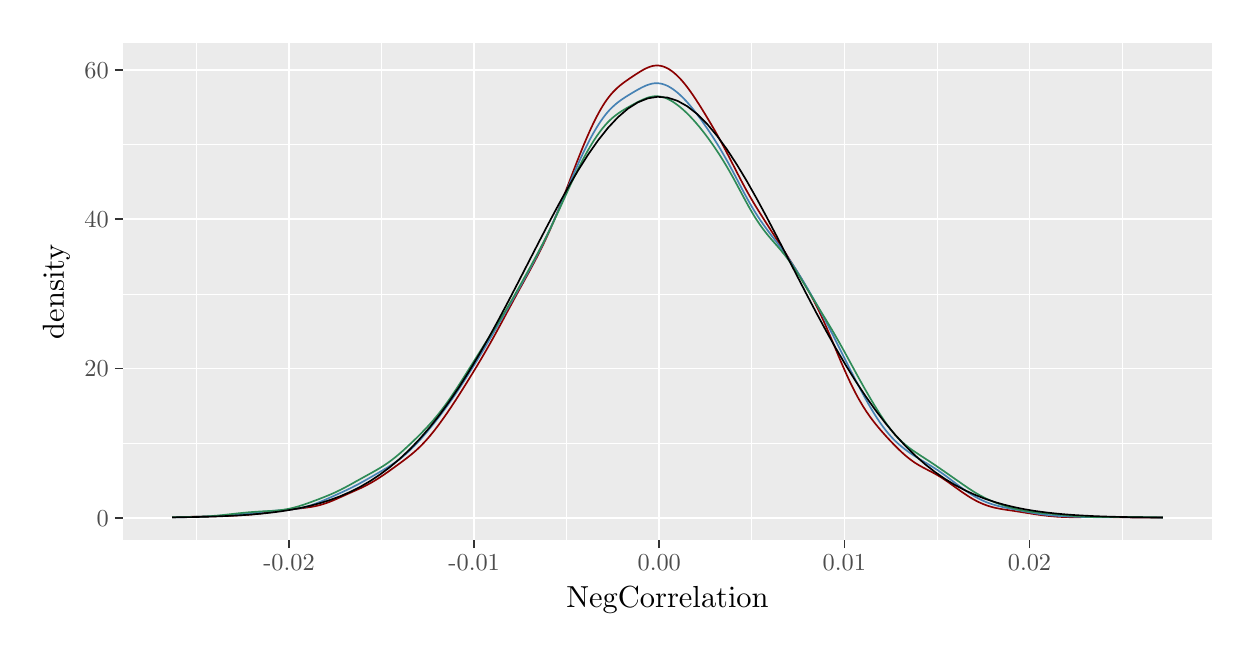
\begin{tikzpicture}[x=1pt,y=1pt]
\definecolor{fillColor}{RGB}{255,255,255}
\path[use as bounding box,fill=fillColor,fill opacity=0.00] (0,0) rectangle (433.62,216.81);
\begin{scope}
\path[clip] (  0.00,  0.00) rectangle (433.62,216.81);
\definecolor{drawColor}{RGB}{255,255,255}
\definecolor{fillColor}{RGB}{255,255,255}

\path[draw=drawColor,line width= 0.6pt,line join=round,line cap=round,fill=fillColor] (  0.00,  0.00) rectangle (433.62,216.81);
\end{scope}
\begin{scope}
\path[clip] ( 34.27, 31.53) rectangle (428.12,211.31);
\definecolor{fillColor}{gray}{0.92}

\path[fill=fillColor] ( 34.27, 31.53) rectangle (428.12,211.31);
\definecolor{drawColor}{RGB}{255,255,255}

\path[draw=drawColor,line width= 0.3pt,line join=round] ( 34.27, 66.67) --
	(428.12, 66.67);

\path[draw=drawColor,line width= 0.3pt,line join=round] ( 34.27,120.60) --
	(428.12,120.60);

\path[draw=drawColor,line width= 0.3pt,line join=round] ( 34.27,174.54) --
	(428.12,174.54);

\path[draw=drawColor,line width= 0.3pt,line join=round] ( 61.01, 31.53) --
	( 61.01,211.31);

\path[draw=drawColor,line width= 0.3pt,line join=round] (127.90, 31.53) --
	(127.90,211.31);

\path[draw=drawColor,line width= 0.3pt,line join=round] (194.78, 31.53) --
	(194.78,211.31);

\path[draw=drawColor,line width= 0.3pt,line join=round] (261.67, 31.53) --
	(261.67,211.31);

\path[draw=drawColor,line width= 0.3pt,line join=round] (328.56, 31.53) --
	(328.56,211.31);

\path[draw=drawColor,line width= 0.3pt,line join=round] (395.45, 31.53) --
	(395.45,211.31);

\path[draw=drawColor,line width= 0.6pt,line join=round] ( 34.27, 39.70) --
	(428.12, 39.70);

\path[draw=drawColor,line width= 0.6pt,line join=round] ( 34.27, 93.64) --
	(428.12, 93.64);

\path[draw=drawColor,line width= 0.6pt,line join=round] ( 34.27,147.57) --
	(428.12,147.57);

\path[draw=drawColor,line width= 0.6pt,line join=round] ( 34.27,201.50) --
	(428.12,201.50);

\path[draw=drawColor,line width= 0.6pt,line join=round] ( 94.45, 31.53) --
	( 94.45,211.31);

\path[draw=drawColor,line width= 0.6pt,line join=round] (161.34, 31.53) --
	(161.34,211.31);

\path[draw=drawColor,line width= 0.6pt,line join=round] (228.23, 31.53) --
	(228.23,211.31);

\path[draw=drawColor,line width= 0.6pt,line join=round] (295.12, 31.53) --
	(295.12,211.31);

\path[draw=drawColor,line width= 0.6pt,line join=round] (362.01, 31.53) --
	(362.01,211.31);
\definecolor{drawColor}{RGB}{139,0,0}

\path[draw=drawColor,line width= 0.6pt,line join=round] ( 52.17, 39.90) --
	( 52.87, 39.92) --
	( 53.57, 39.93) --
	( 54.27, 39.95) --
	( 54.97, 39.97) --
	( 55.67, 39.98) --
	( 56.37, 40.00) --
	( 57.07, 40.01) --
	( 57.78, 40.03) --
	( 58.48, 40.04) --
	( 59.18, 40.06) --
	( 59.88, 40.07) --
	( 60.58, 40.09) --
	( 61.28, 40.11) --
	( 61.98, 40.12) --
	( 62.68, 40.14) --
	( 63.38, 40.15) --
	( 64.08, 40.17) --
	( 64.78, 40.19) --
	( 65.48, 40.20) --
	( 66.18, 40.22) --
	( 66.88, 40.24) --
	( 67.59, 40.26) --
	( 68.29, 40.28) --
	( 68.99, 40.31) --
	( 69.69, 40.33) --
	( 70.39, 40.35) --
	( 71.09, 40.38) --
	( 71.79, 40.40) --
	( 72.49, 40.43) --
	( 73.19, 40.46) --
	( 73.89, 40.49) --
	( 74.59, 40.52) --
	( 75.29, 40.55) --
	( 75.99, 40.58) --
	( 76.69, 40.62) --
	( 77.39, 40.66) --
	( 78.10, 40.70) --
	( 78.80, 40.75) --
	( 79.50, 40.80) --
	( 80.20, 40.85) --
	( 80.90, 40.91) --
	( 81.60, 40.98) --
	( 82.30, 41.05) --
	( 83.00, 41.12) --
	( 83.70, 41.20) --
	( 84.40, 41.29) --
	( 85.10, 41.38) --
	( 85.80, 41.47) --
	( 86.50, 41.57) --
	( 87.20, 41.67) --
	( 87.90, 41.77) --
	( 88.61, 41.87) --
	( 89.31, 41.97) --
	( 90.01, 42.07) --
	( 90.71, 42.17) --
	( 91.41, 42.27) --
	( 92.11, 42.37) --
	( 92.81, 42.46) --
	( 93.51, 42.55) --
	( 94.21, 42.64) --
	( 94.91, 42.72) --
	( 95.61, 42.80) --
	( 96.31, 42.88) --
	( 97.01, 42.96) --
	( 97.71, 43.03) --
	( 98.42, 43.11) --
	( 99.12, 43.19) --
	( 99.82, 43.27) --
	(100.52, 43.35) --
	(101.22, 43.45) --
	(101.92, 43.55) --
	(102.62, 43.66) --
	(103.32, 43.79) --
	(104.02, 43.93) --
	(104.72, 44.09) --
	(105.42, 44.26) --
	(106.12, 44.45) --
	(106.82, 44.67) --
	(107.52, 44.89) --
	(108.22, 45.14) --
	(108.93, 45.41) --
	(109.63, 45.68) --
	(110.33, 45.97) --
	(111.03, 46.27) --
	(111.73, 46.57) --
	(112.43, 46.89) --
	(113.13, 47.20) --
	(113.83, 47.51) --
	(114.53, 47.83) --
	(115.23, 48.14) --
	(115.93, 48.45) --
	(116.63, 48.77) --
	(117.33, 49.08) --
	(118.03, 49.39) --
	(118.73, 49.70) --
	(119.44, 50.02) --
	(120.14, 50.34) --
	(120.84, 50.67) --
	(121.54, 51.01) --
	(122.24, 51.36) --
	(122.94, 51.73) --
	(123.64, 52.11) --
	(124.34, 52.50) --
	(125.04, 52.91) --
	(125.74, 53.33) --
	(126.44, 53.77) --
	(127.14, 54.22) --
	(127.84, 54.69) --
	(128.54, 55.16) --
	(129.24, 55.64) --
	(129.95, 56.13) --
	(130.65, 56.63) --
	(131.35, 57.13) --
	(132.05, 57.63) --
	(132.75, 58.14) --
	(133.45, 58.65) --
	(134.15, 59.16) --
	(134.85, 59.67) --
	(135.55, 60.19) --
	(136.25, 60.72) --
	(136.95, 61.25) --
	(137.65, 61.80) --
	(138.35, 62.36) --
	(139.05, 62.94) --
	(139.76, 63.54) --
	(140.46, 64.16) --
	(141.16, 64.81) --
	(141.86, 65.49) --
	(142.56, 66.19) --
	(143.26, 66.92) --
	(143.96, 67.68) --
	(144.66, 68.47) --
	(145.36, 69.29) --
	(146.06, 70.14) --
	(146.76, 71.01) --
	(147.46, 71.91) --
	(148.16, 72.83) --
	(148.86, 73.77) --
	(149.56, 74.74) --
	(150.27, 75.72) --
	(150.97, 76.71) --
	(151.67, 77.73) --
	(152.37, 78.76) --
	(153.07, 79.80) --
	(153.77, 80.86) --
	(154.47, 81.93) --
	(155.17, 83.01) --
	(155.87, 84.10) --
	(156.57, 85.21) --
	(157.27, 86.32) --
	(157.97, 87.44) --
	(158.67, 88.56) --
	(159.37, 89.70) --
	(160.07, 90.84) --
	(160.78, 91.98) --
	(161.48, 93.14) --
	(162.18, 94.29) --
	(162.88, 95.46) --
	(163.58, 96.63) --
	(164.28, 97.82) --
	(164.98, 99.02) --
	(165.68,100.22) --
	(166.38,101.45) --
	(167.08,102.68) --
	(167.78,103.93) --
	(168.48,105.19) --
	(169.18,106.46) --
	(169.88,107.75) --
	(170.59,109.05) --
	(171.29,110.35) --
	(171.99,111.66) --
	(172.69,112.97) --
	(173.39,114.28) --
	(174.09,115.58) --
	(174.79,116.88) --
	(175.49,118.18) --
	(176.19,119.47) --
	(176.89,120.76) --
	(177.59,122.04) --
	(178.29,123.31) --
	(178.99,124.58) --
	(179.69,125.86) --
	(180.39,127.13) --
	(181.10,128.42) --
	(181.80,129.71) --
	(182.50,131.02) --
	(183.20,132.34) --
	(183.90,133.68) --
	(184.60,135.05) --
	(185.30,136.44) --
	(186.00,137.86) --
	(186.70,139.31) --
	(187.40,140.80) --
	(188.10,142.33) --
	(188.80,143.90) --
	(189.50,145.51) --
	(190.20,147.15) --
	(190.90,148.83) --
	(191.61,150.55) --
	(192.31,152.30) --
	(193.01,154.08) --
	(193.71,155.89) --
	(194.41,157.71) --
	(195.11,159.54) --
	(195.81,161.38) --
	(196.51,163.22) --
	(197.21,165.05) --
	(197.91,166.86) --
	(198.61,168.66) --
	(199.31,170.44) --
	(200.01,172.18) --
	(200.71,173.90) --
	(201.42,175.58) --
	(202.12,177.22) --
	(202.82,178.82) --
	(203.52,180.37) --
	(204.22,181.86) --
	(204.92,183.30) --
	(205.62,184.67) --
	(206.32,185.99) --
	(207.02,187.24) --
	(207.72,188.42) --
	(208.42,189.53) --
	(209.12,190.56) --
	(209.82,191.51) --
	(210.52,192.39) --
	(211.22,193.21) --
	(211.93,193.96) --
	(212.63,194.66) --
	(213.33,195.30) --
	(214.03,195.90) --
	(214.73,196.46) --
	(215.43,196.98) --
	(216.13,197.49) --
	(216.83,197.98) --
	(217.53,198.46) --
	(218.23,198.93) --
	(218.93,199.40) --
	(219.63,199.86) --
	(220.33,200.31) --
	(221.03,200.75) --
	(221.73,201.18) --
	(222.44,201.58) --
	(223.14,201.95) --
	(223.84,202.28) --
	(224.54,202.57) --
	(225.24,202.81) --
	(225.94,202.99) --
	(226.64,203.10) --
	(227.34,203.14) --
	(228.04,203.11) --
	(228.74,203.01) --
	(229.44,202.84) --
	(230.14,202.60) --
	(230.84,202.30) --
	(231.54,201.92) --
	(232.24,201.47) --
	(232.95,200.97) --
	(233.65,200.41) --
	(234.35,199.79) --
	(235.05,199.12) --
	(235.75,198.40) --
	(236.45,197.63) --
	(237.15,196.81) --
	(237.85,195.94) --
	(238.55,195.02) --
	(239.25,194.07) --
	(239.95,193.08) --
	(240.65,192.05) --
	(241.35,191.00) --
	(242.05,189.92) --
	(242.76,188.82) --
	(243.46,187.71) --
	(244.16,186.57) --
	(244.86,185.43) --
	(245.56,184.27) --
	(246.26,183.10) --
	(246.96,181.92) --
	(247.66,180.72) --
	(248.36,179.51) --
	(249.06,178.27) --
	(249.76,177.02) --
	(250.46,175.74) --
	(251.16,174.44) --
	(251.86,173.13) --
	(252.56,171.79) --
	(253.27,170.44) --
	(253.97,169.07) --
	(254.67,167.70) --
	(255.37,166.33) --
	(256.07,164.96) --
	(256.77,163.60) --
	(257.47,162.25) --
	(258.17,160.92) --
	(258.87,159.61) --
	(259.57,158.32) --
	(260.27,157.07) --
	(260.97,155.84) --
	(261.67,154.63) --
	(262.37,153.44) --
	(263.07,152.28) --
	(263.78,151.14) --
	(264.48,150.01) --
	(265.18,148.89) --
	(265.88,147.79) --
	(266.58,146.69) --
	(267.28,145.60) --
	(267.98,144.51) --
	(268.68,143.42) --
	(269.38,142.33) --
	(270.08,141.23) --
	(270.78,140.14) --
	(271.48,139.04) --
	(272.18,137.94) --
	(272.88,136.83) --
	(273.59,135.73) --
	(274.29,134.62) --
	(274.99,133.51) --
	(275.69,132.39) --
	(276.39,131.28) --
	(277.09,130.15) --
	(277.79,129.03) --
	(278.49,127.89) --
	(279.19,126.74) --
	(279.89,125.58) --
	(280.59,124.40) --
	(281.29,123.20) --
	(281.99,121.98) --
	(282.69,120.72) --
	(283.39,119.42) --
	(284.10,118.09) --
	(284.80,116.72) --
	(285.50,115.31) --
	(286.20,113.86) --
	(286.90,112.37) --
	(287.60,110.84) --
	(288.30,109.26) --
	(289.00,107.66) --
	(289.70,106.03) --
	(290.40,104.38) --
	(291.10,102.71) --
	(291.80,101.04) --
	(292.50, 99.36) --
	(293.20, 97.69) --
	(293.90, 96.04) --
	(294.61, 94.42) --
	(295.31, 92.82) --
	(296.01, 91.25) --
	(296.71, 89.73) --
	(297.41, 88.24) --
	(298.11, 86.81) --
	(298.81, 85.42) --
	(299.51, 84.09) --
	(300.21, 82.81) --
	(300.91, 81.59) --
	(301.61, 80.41) --
	(302.31, 79.28) --
	(303.01, 78.20) --
	(303.71, 77.17) --
	(304.41, 76.18) --
	(305.12, 75.23) --
	(305.82, 74.31) --
	(306.52, 73.43) --
	(307.22, 72.58) --
	(307.92, 71.74) --
	(308.62, 70.93) --
	(309.32, 70.14) --
	(310.02, 69.36) --
	(310.72, 68.59) --
	(311.42, 67.84) --
	(312.12, 67.10) --
	(312.82, 66.37) --
	(313.52, 65.65) --
	(314.22, 64.95) --
	(314.93, 64.26) --
	(315.63, 63.60) --
	(316.33, 62.95) --
	(317.03, 62.33) --
	(317.73, 61.74) --
	(318.43, 61.18) --
	(319.13, 60.64) --
	(319.83, 60.13) --
	(320.53, 59.65) --
	(321.23, 59.20) --
	(321.93, 58.78) --
	(322.63, 58.37) --
	(323.33, 57.99) --
	(324.03, 57.61) --
	(324.73, 57.25) --
	(325.44, 56.89) --
	(326.14, 56.53) --
	(326.84, 56.16) --
	(327.54, 55.78) --
	(328.24, 55.39) --
	(328.94, 54.99) --
	(329.64, 54.57) --
	(330.34, 54.13) --
	(331.04, 53.67) --
	(331.74, 53.21) --
	(332.44, 52.72) --
	(333.14, 52.23) --
	(333.84, 51.72) --
	(334.54, 51.22) --
	(335.24, 50.71) --
	(335.95, 50.20) --
	(336.65, 49.70) --
	(337.35, 49.20) --
	(338.05, 48.71) --
	(338.75, 48.24) --
	(339.45, 47.78) --
	(340.15, 47.33) --
	(340.85, 46.90) --
	(341.55, 46.49) --
	(342.25, 46.10) --
	(342.95, 45.73) --
	(343.65, 45.38) --
	(344.35, 45.06) --
	(345.05, 44.76) --
	(345.76, 44.48) --
	(346.46, 44.22) --
	(347.16, 43.98) --
	(347.86, 43.77) --
	(348.56, 43.57) --
	(349.26, 43.39) --
	(349.96, 43.23) --
	(350.66, 43.09) --
	(351.36, 42.95) --
	(352.06, 42.83) --
	(352.76, 42.72) --
	(353.46, 42.61) --
	(354.16, 42.50) --
	(354.86, 42.40) --
	(355.56, 42.30) --
	(356.27, 42.20) --
	(356.97, 42.09) --
	(357.67, 41.99) --
	(358.37, 41.88) --
	(359.07, 41.77) --
	(359.77, 41.66) --
	(360.47, 41.55) --
	(361.17, 41.44) --
	(361.87, 41.33) --
	(362.57, 41.22) --
	(363.27, 41.11) --
	(363.97, 41.00) --
	(364.67, 40.90) --
	(365.37, 40.80) --
	(366.07, 40.70) --
	(366.78, 40.61) --
	(367.48, 40.53) --
	(368.18, 40.45) --
	(368.88, 40.37) --
	(369.58, 40.30) --
	(370.28, 40.23) --
	(370.98, 40.18) --
	(371.68, 40.12) --
	(372.38, 40.08) --
	(373.08, 40.04) --
	(373.78, 40.00) --
	(374.48, 39.98) --
	(375.18, 39.95) --
	(375.88, 39.94) --
	(376.58, 39.92) --
	(377.29, 39.92) --
	(377.99, 39.91) --
	(378.69, 39.92) --
	(379.39, 39.92) --
	(380.09, 39.92) --
	(380.79, 39.93) --
	(381.49, 39.94) --
	(382.19, 39.95) --
	(382.89, 39.95) --
	(383.59, 39.96) --
	(384.29, 39.97) --
	(384.99, 39.97) --
	(385.69, 39.97) --
	(386.39, 39.97) --
	(387.10, 39.97) --
	(387.80, 39.97) --
	(388.50, 39.97) --
	(389.20, 39.96) --
	(389.90, 39.95) --
	(390.60, 39.94) --
	(391.30, 39.94) --
	(392.00, 39.93) --
	(392.70, 39.92) --
	(393.40, 39.91) --
	(394.10, 39.90) --
	(394.80, 39.89) --
	(395.50, 39.87) --
	(396.20, 39.86) --
	(396.90, 39.86) --
	(397.61, 39.85) --
	(398.31, 39.84) --
	(399.01, 39.83) --
	(399.71, 39.83) --
	(400.41, 39.82) --
	(401.11, 39.82) --
	(401.81, 39.81) --
	(402.51, 39.81) --
	(403.21, 39.81) --
	(403.91, 39.81) --
	(404.61, 39.81) --
	(405.31, 39.81) --
	(406.01, 39.82) --
	(406.71, 39.82) --
	(407.41, 39.82) --
	(408.12, 39.82) --
	(408.82, 39.82) --
	(409.52, 39.82) --
	(410.22, 39.82);
\definecolor{drawColor}{RGB}{70,130,180}

\path[draw=drawColor,line width= 0.6pt,line join=round] ( 52.17, 39.85) --
	( 52.87, 39.86) --
	( 53.57, 39.87) --
	( 54.27, 39.88) --
	( 54.97, 39.90) --
	( 55.67, 39.91) --
	( 56.37, 39.92) --
	( 57.07, 39.94) --
	( 57.78, 39.95) --
	( 58.48, 39.97) --
	( 59.18, 39.99) --
	( 59.88, 40.02) --
	( 60.58, 40.04) --
	( 61.28, 40.07) --
	( 61.98, 40.09) --
	( 62.68, 40.12) --
	( 63.38, 40.15) --
	( 64.08, 40.18) --
	( 64.78, 40.21) --
	( 65.48, 40.25) --
	( 66.18, 40.28) --
	( 66.88, 40.31) --
	( 67.59, 40.35) --
	( 68.29, 40.38) --
	( 68.99, 40.42) --
	( 69.69, 40.46) --
	( 70.39, 40.50) --
	( 71.09, 40.54) --
	( 71.79, 40.58) --
	( 72.49, 40.63) --
	( 73.19, 40.67) --
	( 73.89, 40.73) --
	( 74.59, 40.78) --
	( 75.29, 40.84) --
	( 75.99, 40.90) --
	( 76.69, 40.97) --
	( 77.39, 41.04) --
	( 78.10, 41.11) --
	( 78.80, 41.18) --
	( 79.50, 41.26) --
	( 80.20, 41.34) --
	( 80.90, 41.42) --
	( 81.60, 41.50) --
	( 82.30, 41.58) --
	( 83.00, 41.66) --
	( 83.70, 41.74) --
	( 84.40, 41.81) --
	( 85.10, 41.89) --
	( 85.80, 41.96) --
	( 86.50, 42.03) --
	( 87.20, 42.09) --
	( 87.90, 42.15) --
	( 88.61, 42.21) --
	( 89.31, 42.26) --
	( 90.01, 42.31) --
	( 90.71, 42.36) --
	( 91.41, 42.41) --
	( 92.11, 42.46) --
	( 92.81, 42.51) --
	( 93.51, 42.57) --
	( 94.21, 42.63) --
	( 94.91, 42.70) --
	( 95.61, 42.77) --
	( 96.31, 42.86) --
	( 97.01, 42.96) --
	( 97.71, 43.08) --
	( 98.42, 43.21) --
	( 99.12, 43.35) --
	( 99.82, 43.51) --
	(100.52, 43.69) --
	(101.22, 43.89) --
	(101.92, 44.10) --
	(102.62, 44.33) --
	(103.32, 44.57) --
	(104.02, 44.82) --
	(104.72, 45.09) --
	(105.42, 45.37) --
	(106.12, 45.65) --
	(106.82, 45.95) --
	(107.52, 46.25) --
	(108.22, 46.55) --
	(108.93, 46.86) --
	(109.63, 47.17) --
	(110.33, 47.48) --
	(111.03, 47.80) --
	(111.73, 48.11) --
	(112.43, 48.43) --
	(113.13, 48.75) --
	(113.83, 49.07) --
	(114.53, 49.39) --
	(115.23, 49.72) --
	(115.93, 50.05) --
	(116.63, 50.39) --
	(117.33, 50.74) --
	(118.03, 51.10) --
	(118.73, 51.46) --
	(119.44, 51.83) --
	(120.14, 52.21) --
	(120.84, 52.60) --
	(121.54, 52.99) --
	(122.24, 53.38) --
	(122.94, 53.78) --
	(123.64, 54.18) --
	(124.34, 54.58) --
	(125.04, 54.98) --
	(125.74, 55.38) --
	(126.44, 55.79) --
	(127.14, 56.19) --
	(127.84, 56.60) --
	(128.54, 57.02) --
	(129.24, 57.44) --
	(129.95, 57.86) --
	(130.65, 58.30) --
	(131.35, 58.75) --
	(132.05, 59.21) --
	(132.75, 59.69) --
	(133.45, 60.18) --
	(134.15, 60.70) --
	(134.85, 61.25) --
	(135.55, 61.81) --
	(136.25, 62.40) --
	(136.95, 63.01) --
	(137.65, 63.64) --
	(138.35, 64.30) --
	(139.05, 64.99) --
	(139.76, 65.69) --
	(140.46, 66.42) --
	(141.16, 67.17) --
	(141.86, 67.94) --
	(142.56, 68.73) --
	(143.26, 69.53) --
	(143.96, 70.35) --
	(144.66, 71.19) --
	(145.36, 72.04) --
	(146.06, 72.90) --
	(146.76, 73.77) --
	(147.46, 74.66) --
	(148.16, 75.56) --
	(148.86, 76.47) --
	(149.56, 77.39) --
	(150.27, 78.33) --
	(150.97, 79.28) --
	(151.67, 80.24) --
	(152.37, 81.22) --
	(153.07, 82.21) --
	(153.77, 83.22) --
	(154.47, 84.24) --
	(155.17, 85.28) --
	(155.87, 86.33) --
	(156.57, 87.39) --
	(157.27, 88.47) --
	(157.97, 89.55) --
	(158.67, 90.65) --
	(159.37, 91.75) --
	(160.07, 92.87) --
	(160.78, 93.99) --
	(161.48, 95.12) --
	(162.18, 96.25) --
	(162.88, 97.40) --
	(163.58, 98.55) --
	(164.28, 99.71) --
	(164.98,100.88) --
	(165.68,102.05) --
	(166.38,103.23) --
	(167.08,104.42) --
	(167.78,105.61) --
	(168.48,106.81) --
	(169.18,108.01) --
	(169.88,109.21) --
	(170.59,110.42) --
	(171.29,111.63) --
	(171.99,112.84) --
	(172.69,114.05) --
	(173.39,115.26) --
	(174.09,116.48) --
	(174.79,117.69) --
	(175.49,118.91) --
	(176.19,120.14) --
	(176.89,121.37) --
	(177.59,122.61) --
	(178.29,123.86) --
	(178.99,125.11) --
	(179.69,126.37) --
	(180.39,127.64) --
	(181.10,128.93) --
	(181.80,130.22) --
	(182.50,131.53) --
	(183.20,132.85) --
	(183.90,134.19) --
	(184.60,135.55) --
	(185.30,136.93) --
	(186.00,138.33) --
	(186.70,139.75) --
	(187.40,141.20) --
	(188.10,142.68) --
	(188.80,144.19) --
	(189.50,145.73) --
	(190.20,147.29) --
	(190.90,148.88) --
	(191.61,150.49) --
	(192.31,152.13) --
	(193.01,153.78) --
	(193.71,155.44) --
	(194.41,157.10) --
	(195.11,158.77) --
	(195.81,160.43) --
	(196.51,162.09) --
	(197.21,163.72) --
	(197.91,165.34) --
	(198.61,166.93) --
	(199.31,168.49) --
	(200.01,170.02) --
	(200.71,171.51) --
	(201.42,172.97) --
	(202.12,174.38) --
	(202.82,175.75) --
	(203.52,177.08) --
	(204.22,178.36) --
	(204.92,179.58) --
	(205.62,180.75) --
	(206.32,181.87) --
	(207.02,182.93) --
	(207.72,183.93) --
	(208.42,184.87) --
	(209.12,185.76) --
	(209.82,186.58) --
	(210.52,187.34) --
	(211.22,188.04) --
	(211.93,188.69) --
	(212.63,189.30) --
	(213.33,189.86) --
	(214.03,190.39) --
	(214.73,190.89) --
	(215.43,191.36) --
	(216.13,191.81) --
	(216.83,192.25) --
	(217.53,192.68) --
	(218.23,193.10) --
	(218.93,193.52) --
	(219.63,193.93) --
	(220.33,194.33) --
	(221.03,194.72) --
	(221.73,195.09) --
	(222.44,195.44) --
	(223.14,195.76) --
	(223.84,196.05) --
	(224.54,196.29) --
	(225.24,196.49) --
	(225.94,196.64) --
	(226.64,196.72) --
	(227.34,196.74) --
	(228.04,196.70) --
	(228.74,196.60) --
	(229.44,196.44) --
	(230.14,196.21) --
	(230.84,195.93) --
	(231.54,195.59) --
	(232.24,195.18) --
	(232.95,194.73) --
	(233.65,194.24) --
	(234.35,193.69) --
	(235.05,193.11) --
	(235.75,192.49) --
	(236.45,191.82) --
	(237.15,191.12) --
	(237.85,190.38) --
	(238.55,189.61) --
	(239.25,188.80) --
	(239.95,187.96) --
	(240.65,187.09) --
	(241.35,186.20) --
	(242.05,185.28) --
	(242.76,184.33) --
	(243.46,183.37) --
	(244.16,182.38) --
	(244.86,181.37) --
	(245.56,180.35) --
	(246.26,179.31) --
	(246.96,178.25) --
	(247.66,177.18) --
	(248.36,176.08) --
	(249.06,174.96) --
	(249.76,173.82) --
	(250.46,172.65) --
	(251.16,171.45) --
	(251.86,170.23) --
	(252.56,168.99) --
	(253.27,167.72) --
	(253.97,166.42) --
	(254.67,165.11) --
	(255.37,163.78) --
	(256.07,162.45) --
	(256.77,161.11) --
	(257.47,159.77) --
	(258.17,158.44) --
	(258.87,157.12) --
	(259.57,155.83) --
	(260.27,154.56) --
	(260.97,153.32) --
	(261.67,152.11) --
	(262.37,150.94) --
	(263.07,149.80) --
	(263.78,148.70) --
	(264.48,147.64) --
	(265.18,146.61) --
	(265.88,145.61) --
	(266.58,144.64) --
	(267.28,143.69) --
	(267.98,142.76) --
	(268.68,141.84) --
	(269.38,140.93) --
	(270.08,140.02) --
	(270.78,139.10) --
	(271.48,138.18) --
	(272.18,137.25) --
	(272.88,136.30) --
	(273.59,135.34) --
	(274.29,134.35) --
	(274.99,133.35) --
	(275.69,132.32) --
	(276.39,131.28) --
	(277.09,130.21) --
	(277.79,129.13) --
	(278.49,128.02) --
	(279.19,126.90) --
	(279.89,125.76) --
	(280.59,124.60) --
	(281.29,123.43) --
	(281.99,122.24) --
	(282.69,121.03) --
	(283.39,119.81) --
	(284.10,118.58) --
	(284.80,117.33) --
	(285.50,116.06) --
	(286.20,114.78) --
	(286.90,113.49) --
	(287.60,112.18) --
	(288.30,110.86) --
	(289.00,109.52) --
	(289.70,108.17) --
	(290.40,106.81) --
	(291.10,105.44) --
	(291.80,104.06) --
	(292.50,102.67) --
	(293.20,101.28) --
	(293.90, 99.88) --
	(294.61, 98.48) --
	(295.31, 97.07) --
	(296.01, 95.68) --
	(296.71, 94.28) --
	(297.41, 92.89) --
	(298.11, 91.51) --
	(298.81, 90.14) --
	(299.51, 88.79) --
	(300.21, 87.44) --
	(300.91, 86.11) --
	(301.61, 84.80) --
	(302.31, 83.51) --
	(303.01, 82.25) --
	(303.71, 81.00) --
	(304.41, 79.79) --
	(305.12, 78.61) --
	(305.82, 77.45) --
	(306.52, 76.34) --
	(307.22, 75.26) --
	(307.92, 74.22) --
	(308.62, 73.23) --
	(309.32, 72.28) --
	(310.02, 71.37) --
	(310.72, 70.50) --
	(311.42, 69.68) --
	(312.12, 68.89) --
	(312.82, 68.15) --
	(313.52, 67.45) --
	(314.22, 66.79) --
	(314.93, 66.15) --
	(315.63, 65.55) --
	(316.33, 64.98) --
	(317.03, 64.43) --
	(317.73, 63.91) --
	(318.43, 63.41) --
	(319.13, 62.92) --
	(319.83, 62.46) --
	(320.53, 62.00) --
	(321.23, 61.56) --
	(321.93, 61.13) --
	(322.63, 60.71) --
	(323.33, 60.29) --
	(324.03, 59.87) --
	(324.73, 59.46) --
	(325.44, 59.04) --
	(326.14, 58.61) --
	(326.84, 58.18) --
	(327.54, 57.74) --
	(328.24, 57.29) --
	(328.94, 56.83) --
	(329.64, 56.35) --
	(330.34, 55.86) --
	(331.04, 55.36) --
	(331.74, 54.85) --
	(332.44, 54.33) --
	(333.14, 53.81) --
	(333.84, 53.28) --
	(334.54, 52.74) --
	(335.24, 52.21) --
	(335.95, 51.68) --
	(336.65, 51.15) --
	(337.35, 50.63) --
	(338.05, 50.13) --
	(338.75, 49.63) --
	(339.45, 49.15) --
	(340.15, 48.68) --
	(340.85, 48.24) --
	(341.55, 47.81) --
	(342.25, 47.40) --
	(342.95, 47.01) --
	(343.65, 46.63) --
	(344.35, 46.28) --
	(345.05, 45.95) --
	(345.76, 45.64) --
	(346.46, 45.35) --
	(347.16, 45.08) --
	(347.86, 44.83) --
	(348.56, 44.60) --
	(349.26, 44.38) --
	(349.96, 44.18) --
	(350.66, 43.99) --
	(351.36, 43.82) --
	(352.06, 43.65) --
	(352.76, 43.49) --
	(353.46, 43.34) --
	(354.16, 43.20) --
	(354.86, 43.06) --
	(355.56, 42.92) --
	(356.27, 42.78) --
	(356.97, 42.65) --
	(357.67, 42.51) --
	(358.37, 42.38) --
	(359.07, 42.24) --
	(359.77, 42.11) --
	(360.47, 41.97) --
	(361.17, 41.84) --
	(361.87, 41.71) --
	(362.57, 41.58) --
	(363.27, 41.46) --
	(363.97, 41.34) --
	(364.67, 41.22) --
	(365.37, 41.11) --
	(366.07, 41.01) --
	(366.78, 40.92) --
	(367.48, 40.83) --
	(368.18, 40.75) --
	(368.88, 40.67) --
	(369.58, 40.60) --
	(370.28, 40.54) --
	(370.98, 40.48) --
	(371.68, 40.43) --
	(372.38, 40.38) --
	(373.08, 40.34) --
	(373.78, 40.30) --
	(374.48, 40.26) --
	(375.18, 40.22) --
	(375.88, 40.19) --
	(376.58, 40.16) --
	(377.29, 40.13) --
	(377.99, 40.11) --
	(378.69, 40.08) --
	(379.39, 40.06) --
	(380.09, 40.04) --
	(380.79, 40.01) --
	(381.49, 40.00) --
	(382.19, 39.98) --
	(382.89, 39.96) --
	(383.59, 39.95) --
	(384.29, 39.94) --
	(384.99, 39.93) --
	(385.69, 39.92) --
	(386.39, 39.92) --
	(387.10, 39.92) --
	(387.80, 39.92) --
	(388.50, 39.92) --
	(389.20, 39.92) --
	(389.90, 39.92) --
	(390.60, 39.92) --
	(391.30, 39.92) --
	(392.00, 39.93) --
	(392.70, 39.93) --
	(393.40, 39.93) --
	(394.10, 39.93) --
	(394.80, 39.93) --
	(395.50, 39.93) --
	(396.20, 39.92) --
	(396.90, 39.92) --
	(397.61, 39.92) --
	(398.31, 39.91) --
	(399.01, 39.91) --
	(399.71, 39.90) --
	(400.41, 39.90) --
	(401.11, 39.89) --
	(401.81, 39.89) --
	(402.51, 39.88) --
	(403.21, 39.87) --
	(403.91, 39.87) --
	(404.61, 39.86) --
	(405.31, 39.86) --
	(406.01, 39.86) --
	(406.71, 39.85) --
	(407.41, 39.85) --
	(408.12, 39.84) --
	(408.82, 39.83) --
	(409.52, 39.83) --
	(410.22, 39.82);
\definecolor{drawColor}{RGB}{46,139,87}

\path[draw=drawColor,line width= 0.6pt,line join=round] ( 52.17, 39.91) --
	( 52.87, 39.92) --
	( 53.57, 39.93) --
	( 54.27, 39.95) --
	( 54.97, 39.96) --
	( 55.67, 39.97) --
	( 56.37, 39.98) --
	( 57.07, 39.99) --
	( 57.78, 40.01) --
	( 58.48, 40.02) --
	( 59.18, 40.03) --
	( 59.88, 40.05) --
	( 60.58, 40.07) --
	( 61.28, 40.09) --
	( 61.98, 40.11) --
	( 62.68, 40.13) --
	( 63.38, 40.16) --
	( 64.08, 40.19) --
	( 64.78, 40.23) --
	( 65.48, 40.27) --
	( 66.18, 40.32) --
	( 66.88, 40.37) --
	( 67.59, 40.43) --
	( 68.29, 40.49) --
	( 68.99, 40.55) --
	( 69.69, 40.62) --
	( 70.39, 40.69) --
	( 71.09, 40.77) --
	( 71.79, 40.84) --
	( 72.49, 40.92) --
	( 73.19, 41.00) --
	( 73.89, 41.08) --
	( 74.59, 41.15) --
	( 75.29, 41.23) --
	( 75.99, 41.31) --
	( 76.69, 41.38) --
	( 77.39, 41.46) --
	( 78.10, 41.53) --
	( 78.80, 41.59) --
	( 79.50, 41.66) --
	( 80.20, 41.72) --
	( 80.90, 41.77) --
	( 81.60, 41.83) --
	( 82.30, 41.88) --
	( 83.00, 41.93) --
	( 83.70, 41.97) --
	( 84.40, 42.01) --
	( 85.10, 42.05) --
	( 85.80, 42.08) --
	( 86.50, 42.12) --
	( 87.20, 42.16) --
	( 87.90, 42.20) --
	( 88.61, 42.24) --
	( 89.31, 42.29) --
	( 90.01, 42.35) --
	( 90.71, 42.42) --
	( 91.41, 42.49) --
	( 92.11, 42.58) --
	( 92.81, 42.69) --
	( 93.51, 42.80) --
	( 94.21, 42.93) --
	( 94.91, 43.08) --
	( 95.61, 43.24) --
	( 96.31, 43.42) --
	( 97.01, 43.61) --
	( 97.71, 43.81) --
	( 98.42, 44.02) --
	( 99.12, 44.25) --
	( 99.82, 44.48) --
	(100.52, 44.72) --
	(101.22, 44.97) --
	(101.92, 45.22) --
	(102.62, 45.48) --
	(103.32, 45.74) --
	(104.02, 46.00) --
	(104.72, 46.26) --
	(105.42, 46.53) --
	(106.12, 46.80) --
	(106.82, 47.08) --
	(107.52, 47.36) --
	(108.22, 47.64) --
	(108.93, 47.93) --
	(109.63, 48.23) --
	(110.33, 48.54) --
	(111.03, 48.85) --
	(111.73, 49.18) --
	(112.43, 49.52) --
	(113.13, 49.86) --
	(113.83, 50.22) --
	(114.53, 50.59) --
	(115.23, 50.96) --
	(115.93, 51.34) --
	(116.63, 51.72) --
	(117.33, 52.11) --
	(118.03, 52.50) --
	(118.73, 52.90) --
	(119.44, 53.29) --
	(120.14, 53.68) --
	(120.84, 54.07) --
	(121.54, 54.45) --
	(122.24, 54.84) --
	(122.94, 55.23) --
	(123.64, 55.61) --
	(124.34, 56.00) --
	(125.04, 56.39) --
	(125.74, 56.79) --
	(126.44, 57.19) --
	(127.14, 57.61) --
	(127.84, 58.04) --
	(128.54, 58.48) --
	(129.24, 58.94) --
	(129.95, 59.42) --
	(130.65, 59.91) --
	(131.35, 60.43) --
	(132.05, 60.97) --
	(132.75, 61.52) --
	(133.45, 62.09) --
	(134.15, 62.68) --
	(134.85, 63.29) --
	(135.55, 63.90) --
	(136.25, 64.54) --
	(136.95, 65.18) --
	(137.65, 65.83) --
	(138.35, 66.49) --
	(139.05, 67.16) --
	(139.76, 67.83) --
	(140.46, 68.52) --
	(141.16, 69.21) --
	(141.86, 69.91) --
	(142.56, 70.62) --
	(143.26, 71.34) --
	(143.96, 72.08) --
	(144.66, 72.83) --
	(145.36, 73.60) --
	(146.06, 74.38) --
	(146.76, 75.19) --
	(147.46, 76.02) --
	(148.16, 76.88) --
	(148.86, 77.76) --
	(149.56, 78.66) --
	(150.27, 79.59) --
	(150.97, 80.54) --
	(151.67, 81.51) --
	(152.37, 82.51) --
	(153.07, 83.53) --
	(153.77, 84.56) --
	(154.47, 85.62) --
	(155.17, 86.69) --
	(155.87, 87.77) --
	(156.57, 88.86) --
	(157.27, 89.96) --
	(157.97, 91.07) --
	(158.67, 92.18) --
	(159.37, 93.30) --
	(160.07, 94.41) --
	(160.78, 95.53) --
	(161.48, 96.65) --
	(162.18, 97.77) --
	(162.88, 98.88) --
	(163.58, 99.99) --
	(164.28,101.10) --
	(164.98,102.21) --
	(165.68,103.31) --
	(166.38,104.42) --
	(167.08,105.52) --
	(167.78,106.63) --
	(168.48,107.74) --
	(169.18,108.86) --
	(169.88,109.99) --
	(170.59,111.12) --
	(171.29,112.26) --
	(171.99,113.42) --
	(172.69,114.58) --
	(173.39,115.77) --
	(174.09,116.96) --
	(174.79,118.16) --
	(175.49,119.38) --
	(176.19,120.61) --
	(176.89,121.85) --
	(177.59,123.09) --
	(178.29,124.35) --
	(178.99,125.61) --
	(179.69,126.87) --
	(180.39,128.14) --
	(181.10,129.41) --
	(181.80,130.69) --
	(182.50,131.97) --
	(183.20,133.26) --
	(183.90,134.56) --
	(184.60,135.87) --
	(185.30,137.19) --
	(186.00,138.53) --
	(186.70,139.89) --
	(187.40,141.27) --
	(188.10,142.68) --
	(188.80,144.11) --
	(189.50,145.56) --
	(190.20,147.04) --
	(190.90,148.54) --
	(191.61,150.06) --
	(192.31,151.59) --
	(193.01,153.13) --
	(193.71,154.68) --
	(194.41,156.23) --
	(195.11,157.77) --
	(195.81,159.30) --
	(196.51,160.81) --
	(197.21,162.30) --
	(197.91,163.77) --
	(198.61,165.21) --
	(199.31,166.62) --
	(200.01,167.99) --
	(200.71,169.32) --
	(201.42,170.62) --
	(202.12,171.89) --
	(202.82,173.11) --
	(203.52,174.30) --
	(204.22,175.44) --
	(204.92,176.54) --
	(205.62,177.58) --
	(206.32,178.58) --
	(207.02,179.53) --
	(207.72,180.43) --
	(208.42,181.28) --
	(209.12,182.07) --
	(209.82,182.82) --
	(210.52,183.50) --
	(211.22,184.13) --
	(211.93,184.72) --
	(212.63,185.27) --
	(213.33,185.78) --
	(214.03,186.26) --
	(214.73,186.72) --
	(215.43,187.15) --
	(216.13,187.56) --
	(216.83,187.97) --
	(217.53,188.36) --
	(218.23,188.75) --
	(218.93,189.13) --
	(219.63,189.51) --
	(220.33,189.88) --
	(221.03,190.23) --
	(221.73,190.57) --
	(222.44,190.89) --
	(223.14,191.18) --
	(223.84,191.44) --
	(224.54,191.66) --
	(225.24,191.83) --
	(225.94,191.96) --
	(226.64,192.03) --
	(227.34,192.04) --
	(228.04,191.99) --
	(228.74,191.89) --
	(229.44,191.73) --
	(230.14,191.51) --
	(230.84,191.24) --
	(231.54,190.92) --
	(232.24,190.55) --
	(232.95,190.14) --
	(233.65,189.68) --
	(234.35,189.19) --
	(235.05,188.67) --
	(235.75,188.11) --
	(236.45,187.52) --
	(237.15,186.90) --
	(237.85,186.25) --
	(238.55,185.56) --
	(239.25,184.86) --
	(239.95,184.12) --
	(240.65,183.36) --
	(241.35,182.57) --
	(242.05,181.75) --
	(242.76,180.91) --
	(243.46,180.04) --
	(244.16,179.15) --
	(244.86,178.24) --
	(245.56,177.30) --
	(246.26,176.35) --
	(246.96,175.37) --
	(247.66,174.38) --
	(248.36,173.36) --
	(249.06,172.31) --
	(249.76,171.25) --
	(250.46,170.15) --
	(251.16,169.04) --
	(251.86,167.89) --
	(252.56,166.72) --
	(253.27,165.51) --
	(253.97,164.28) --
	(254.67,163.03) --
	(255.37,161.76) --
	(256.07,160.47) --
	(256.77,159.16) --
	(257.47,157.85) --
	(258.17,156.54) --
	(258.87,155.23) --
	(259.57,153.94) --
	(260.27,152.67) --
	(260.97,151.42) --
	(261.67,150.21) --
	(262.37,149.03) --
	(263.07,147.90) --
	(263.78,146.82) --
	(264.48,145.78) --
	(265.18,144.79) --
	(265.88,143.84) --
	(266.58,142.93) --
	(267.28,142.05) --
	(267.98,141.21) --
	(268.68,140.39) --
	(269.38,139.59) --
	(270.08,138.79) --
	(270.78,137.99) --
	(271.48,137.18) --
	(272.18,136.35) --
	(272.88,135.50) --
	(273.59,134.63) --
	(274.29,133.72) --
	(274.99,132.77) --
	(275.69,131.79) --
	(276.39,130.78) --
	(277.09,129.74) --
	(277.79,128.67) --
	(278.49,127.58) --
	(279.19,126.46) --
	(279.89,125.32) --
	(280.59,124.18) --
	(281.29,123.02) --
	(281.99,121.87) --
	(282.69,120.71) --
	(283.39,119.55) --
	(284.10,118.40) --
	(284.80,117.25) --
	(285.50,116.10) --
	(286.20,114.96) --
	(286.90,113.81) --
	(287.60,112.67) --
	(288.30,111.52) --
	(289.00,110.36) --
	(289.70,109.20) --
	(290.40,108.02) --
	(291.10,106.83) --
	(291.80,105.62) --
	(292.50,104.40) --
	(293.20,103.17) --
	(293.90,101.92) --
	(294.61,100.66) --
	(295.31, 99.39) --
	(296.01, 98.11) --
	(296.71, 96.82) --
	(297.41, 95.53) --
	(298.11, 94.24) --
	(298.81, 92.96) --
	(299.51, 91.68) --
	(300.21, 90.40) --
	(300.91, 89.14) --
	(301.61, 87.89) --
	(302.31, 86.64) --
	(303.01, 85.42) --
	(303.71, 84.20) --
	(304.41, 83.00) --
	(305.12, 81.81) --
	(305.82, 80.64) --
	(306.52, 79.49) --
	(307.22, 78.37) --
	(307.92, 77.26) --
	(308.62, 76.18) --
	(309.32, 75.13) --
	(310.02, 74.12) --
	(310.72, 73.13) --
	(311.42, 72.19) --
	(312.12, 71.30) --
	(312.82, 70.44) --
	(313.52, 69.63) --
	(314.22, 68.86) --
	(314.93, 68.13) --
	(315.63, 67.44) --
	(316.33, 66.80) --
	(317.03, 66.20) --
	(317.73, 65.63) --
	(318.43, 65.08) --
	(319.13, 64.56) --
	(319.83, 64.06) --
	(320.53, 63.58) --
	(321.23, 63.11) --
	(321.93, 62.65) --
	(322.63, 62.19) --
	(323.33, 61.74) --
	(324.03, 61.28) --
	(324.73, 60.83) --
	(325.44, 60.37) --
	(326.14, 59.91) --
	(326.84, 59.44) --
	(327.54, 58.97) --
	(328.24, 58.50) --
	(328.94, 58.02) --
	(329.64, 57.54) --
	(330.34, 57.06) --
	(331.04, 56.58) --
	(331.74, 56.09) --
	(332.44, 55.60) --
	(333.14, 55.11) --
	(333.84, 54.62) --
	(334.54, 54.13) --
	(335.24, 53.64) --
	(335.95, 53.14) --
	(336.65, 52.65) --
	(337.35, 52.16) --
	(338.05, 51.68) --
	(338.75, 51.20) --
	(339.45, 50.72) --
	(340.15, 50.25) --
	(340.85, 49.80) --
	(341.55, 49.35) --
	(342.25, 48.91) --
	(342.95, 48.49) --
	(343.65, 48.09) --
	(344.35, 47.69) --
	(345.05, 47.32) --
	(345.76, 46.96) --
	(346.46, 46.61) --
	(347.16, 46.28) --
	(347.86, 45.97) --
	(348.56, 45.67) --
	(349.26, 45.38) --
	(349.96, 45.11) --
	(350.66, 44.84) --
	(351.36, 44.59) --
	(352.06, 44.35) --
	(352.76, 44.12) --
	(353.46, 43.90) --
	(354.16, 43.69) --
	(354.86, 43.48) --
	(355.56, 43.29) --
	(356.27, 43.11) --
	(356.97, 42.93) --
	(357.67, 42.77) --
	(358.37, 42.61) --
	(359.07, 42.47) --
	(359.77, 42.33) --
	(360.47, 42.21) --
	(361.17, 42.09) --
	(361.87, 41.98) --
	(362.57, 41.89) --
	(363.27, 41.79) --
	(363.97, 41.71) --
	(364.67, 41.63) --
	(365.37, 41.56) --
	(366.07, 41.49) --
	(366.78, 41.42) --
	(367.48, 41.35) --
	(368.18, 41.29) --
	(368.88, 41.22) --
	(369.58, 41.16) --
	(370.28, 41.10) --
	(370.98, 41.03) --
	(371.68, 40.97) --
	(372.38, 40.90) --
	(373.08, 40.83) --
	(373.78, 40.76) --
	(374.48, 40.70) --
	(375.18, 40.63) --
	(375.88, 40.56) --
	(376.58, 40.50) --
	(377.29, 40.44) --
	(377.99, 40.38) --
	(378.69, 40.32) --
	(379.39, 40.27) --
	(380.09, 40.22) --
	(380.79, 40.17) --
	(381.49, 40.13) --
	(382.19, 40.10) --
	(382.89, 40.06) --
	(383.59, 40.03) --
	(384.29, 40.01) --
	(384.99, 39.99) --
	(385.69, 39.97) --
	(386.39, 39.96) --
	(387.10, 39.95) --
	(387.80, 39.94) --
	(388.50, 39.94) --
	(389.20, 39.94) --
	(389.90, 39.94) --
	(390.60, 39.94) --
	(391.30, 39.94) --
	(392.00, 39.95) --
	(392.70, 39.95) --
	(393.40, 39.96) --
	(394.10, 39.97) --
	(394.80, 39.97) --
	(395.50, 39.98) --
	(396.20, 39.98) --
	(396.90, 39.99) --
	(397.61, 39.99) --
	(398.31, 39.99) --
	(399.01, 39.99) --
	(399.71, 39.99) --
	(400.41, 39.99) --
	(401.11, 39.98) --
	(401.81, 39.98) --
	(402.51, 39.97) --
	(403.21, 39.96) --
	(403.91, 39.95) --
	(404.61, 39.94) --
	(405.31, 39.93) --
	(406.01, 39.91) --
	(406.71, 39.90) --
	(407.41, 39.89) --
	(408.12, 39.87) --
	(408.82, 39.86) --
	(409.52, 39.84) --
	(410.22, 39.83);
\definecolor{drawColor}{RGB}{0,0,0}

\path[draw=drawColor,line width= 0.6pt,line join=round] ( 52.17, 39.85) --
	( 55.75, 39.90) --
	( 59.33, 39.96) --
	( 62.91, 40.04) --
	( 66.49, 40.14) --
	( 70.07, 40.27) --
	( 73.65, 40.43) --
	( 77.23, 40.63) --
	( 80.81, 40.89) --
	( 84.39, 41.20) --
	( 87.97, 41.58) --
	( 91.56, 42.04) --
	( 95.14, 42.61) --
	( 98.72, 43.28) --
	(102.30, 44.10) --
	(105.88, 45.06) --
	(109.46, 46.20) --
	(113.04, 47.54) --
	(116.62, 49.10) --
	(120.20, 50.91) --
	(123.78, 52.99) --
	(127.36, 55.36) --
	(130.94, 58.05) --
	(134.52, 61.08) --
	(138.10, 64.46) --
	(141.68, 68.22) --
	(145.26, 72.37) --
	(148.84, 76.90) --
	(152.42, 81.82) --
	(156.00, 87.12) --
	(159.58, 92.77) --
	(163.16, 98.77) --
	(166.75,105.06) --
	(170.33,111.62) --
	(173.91,118.37) --
	(177.49,125.27) --
	(181.07,132.25) --
	(184.65,139.22) --
	(188.23,146.10) --
	(191.81,152.81) --
	(195.39,159.26) --
	(198.97,165.35) --
	(202.55,171.00) --
	(206.13,176.11) --
	(209.71,180.62) --
	(213.29,184.45) --
	(216.87,187.52) --
	(220.45,189.80) --
	(224.03,191.25) --
	(227.61,191.83) --
	(231.19,191.55) --
	(234.77,190.40) --
	(238.35,188.40) --
	(241.94,185.59) --
	(245.52,182.01) --
	(249.10,177.73) --
	(252.68,172.82) --
	(256.26,167.34) --
	(259.84,161.40) --
	(263.42,155.06) --
	(267.00,148.43) --
	(270.58,141.60) --
	(274.16,134.65) --
	(277.74,127.66) --
	(281.32,120.73) --
	(284.90,113.92) --
	(288.48,107.29) --
	(292.06,100.90) --
	(295.64, 94.80) --
	(299.22, 89.02) --
	(302.80, 83.60) --
	(306.38, 78.55) --
	(309.96, 73.88) --
	(313.54, 69.60) --
	(317.13, 65.71) --
	(320.71, 62.20) --
	(324.29, 59.05) --
	(327.87, 56.24) --
	(331.45, 53.76) --
	(335.03, 51.59) --
	(338.61, 49.69) --
	(342.19, 48.05) --
	(345.77, 46.64) --
	(349.35, 45.43) --
	(352.93, 44.41) --
	(356.51, 43.55) --
	(360.09, 42.82) --
	(363.67, 42.22) --
	(367.25, 41.73) --
	(370.83, 41.32) --
	(374.41, 40.98) --
	(377.99, 40.71) --
	(381.57, 40.50) --
	(385.15, 40.32) --
	(388.73, 40.18) --
	(392.32, 40.07) --
	(395.90, 39.99) --
	(399.48, 39.92) --
	(403.06, 39.87) --
	(406.64, 39.83) --
	(410.22, 39.80);
\end{scope}
\begin{scope}
\path[clip] (  0.00,  0.00) rectangle (433.62,216.81);
\definecolor{drawColor}{gray}{0.30}

\node[text=drawColor,anchor=base east,inner sep=0pt, outer sep=0pt, scale=  0.88] at ( 29.32, 36.67) {0};

\node[text=drawColor,anchor=base east,inner sep=0pt, outer sep=0pt, scale=  0.88] at ( 29.32, 90.61) {20};

\node[text=drawColor,anchor=base east,inner sep=0pt, outer sep=0pt, scale=  0.88] at ( 29.32,144.54) {40};

\node[text=drawColor,anchor=base east,inner sep=0pt, outer sep=0pt, scale=  0.88] at ( 29.32,198.47) {60};
\end{scope}
\begin{scope}
\path[clip] (  0.00,  0.00) rectangle (433.62,216.81);
\definecolor{drawColor}{gray}{0.20}

\path[draw=drawColor,line width= 0.6pt,line join=round] ( 31.52, 39.70) --
	( 34.27, 39.70);

\path[draw=drawColor,line width= 0.6pt,line join=round] ( 31.52, 93.64) --
	( 34.27, 93.64);

\path[draw=drawColor,line width= 0.6pt,line join=round] ( 31.52,147.57) --
	( 34.27,147.57);

\path[draw=drawColor,line width= 0.6pt,line join=round] ( 31.52,201.50) --
	( 34.27,201.50);
\end{scope}
\begin{scope}
\path[clip] (  0.00,  0.00) rectangle (433.62,216.81);
\definecolor{drawColor}{gray}{0.20}

\path[draw=drawColor,line width= 0.6pt,line join=round] ( 94.45, 28.78) --
	( 94.45, 31.53);

\path[draw=drawColor,line width= 0.6pt,line join=round] (161.34, 28.78) --
	(161.34, 31.53);

\path[draw=drawColor,line width= 0.6pt,line join=round] (228.23, 28.78) --
	(228.23, 31.53);

\path[draw=drawColor,line width= 0.6pt,line join=round] (295.12, 28.78) --
	(295.12, 31.53);

\path[draw=drawColor,line width= 0.6pt,line join=round] (362.01, 28.78) --
	(362.01, 31.53);
\end{scope}
\begin{scope}
\path[clip] (  0.00,  0.00) rectangle (433.62,216.81);
\definecolor{drawColor}{gray}{0.30}

\node[text=drawColor,anchor=base,inner sep=0pt, outer sep=0pt, scale=  0.88] at ( 94.45, 20.52) {-0.02};

\node[text=drawColor,anchor=base,inner sep=0pt, outer sep=0pt, scale=  0.88] at (161.34, 20.52) {-0.01};

\node[text=drawColor,anchor=base,inner sep=0pt, outer sep=0pt, scale=  0.88] at (228.23, 20.52) {0.00};

\node[text=drawColor,anchor=base,inner sep=0pt, outer sep=0pt, scale=  0.88] at (295.12, 20.52) {0.01};

\node[text=drawColor,anchor=base,inner sep=0pt, outer sep=0pt, scale=  0.88] at (362.01, 20.52) {0.02};
\end{scope}
\begin{scope}
\path[clip] (  0.00,  0.00) rectangle (433.62,216.81);
\definecolor{drawColor}{RGB}{0,0,0}

\node[text=drawColor,anchor=base,inner sep=0pt, outer sep=0pt, scale=  1.10] at (231.19,  7.44) {NegCorrelation};
\end{scope}
\begin{scope}
\path[clip] (  0.00,  0.00) rectangle (433.62,216.81);
\definecolor{drawColor}{RGB}{0,0,0}

\node[text=drawColor,rotate= 90.00,anchor=base,inner sep=0pt, outer sep=0pt, scale=  1.10] at ( 13.08,121.42) {density};
\end{scope}
\end{tikzpicture}

\caption{Merton: Log--return skewness on Heston}
\floatfoot{The above densities function (red, blue and green) are constructed over three distinctive groups of 10000 samples each. The black curve density is theoretical.
All samples are generated by an algorithm based on \cref{eq:other:hsvstock} for the stock data and on \cref{eq:other:hsvvol} for the related volatility (see function \textit{heston()} on appendix \ref{sub:r:time:heston} for more information). The only parameter that changes over the groups is $\sigma$ which is set to 0, 0.2, 0.4. The log-return densities of these groups are respectively represented by the green, blue and red outlined density curves. 
The black density represents to the normal bell curve with mean $- \frac{\theta}{2}$ and standard deviation of $\sqrt{\theta}$. The log-price return cover a period of one year with a time step of 500.
}
\label{p:other:heston:kurtosis}
\end{figure}




%%%%%%%%%%%%%%%%%%%%%%%%%%%%%%%%%%%%%%%%%%%%%%%%
% SECTION: Option pricing method
%%%%%%%%%%%%%%%%%%%%%%%%%%%%%%%%%%%%%%%%%%%%%%%%
\section{Option pricing method}
\label{sec:other:option}

As shown by \cref{sec:other:merton} and \cref{sec:other:heston}, the frameworks developed by \citet{merton76} and \citet{heston1993} drastically change the distribution of any underlying assets following such processes. Therefore, the pricing method to be used must also be adapted in order to take that update into account.

In his paper, \citet{heston1993} developed a techinque to price options using the characteristic function of the underlying asset. Furthermore, according to \citet{criso2015} that method could be used to price every options provided that the underlying's characteristic  is known.

\subsection{Probabilistic approach}
\label{sub:other:option:probabilistic}

\citet{heston1993} proposed the solution given by \cref{eq:other:call:heston} to price a european call option.

\begin{align}
  C(t) = S(t) P_1 - e^{-r(T-t)} K P_2 \label{eq:other:call:heston}
\end{align}

Through this method, the european call price at time $t$, namely $C(t)$, is computed thanks to \cref{eq:other:call:heston}, where $S(t)$ and $e^{r(T - t)}$ respectively stand for the stock price and the present value of the strike at that time $t$.

\begin{align}
  P_1(x,V,t;\ln{K}) &= \frac{1}{2} + \frac{1}{\pi} \int_0^{\infty} Re \left( \frac{e^{-i\phi\ln{K}} \psi(x,V,t;\phi - i)}{i\phi\psi(x,V,t;-i)} \right) d\phi \label{eq:other:call:heston:pi1} \\ 
  \intertext{}
  P_2(x,V,t;\ln{K}) &= \frac{1}{2} + \frac{1}{\pi} \int_0^{\infty} Re \left( \frac{e^{-i\phi\ln{K}} \psi(x,V,t;\phi)}{i\phi} \right) d\phi \label{eq:other:call:heston:pi2}
\end{align}

Following the development in \citet{criso2015}, \Cref{eq:other:call:heston:pi} both are probability quantities that involve the underlying characteristic function, namely $\psi(x,V,t;\phi)$. Once these quantities are computed, they are substituted in \cref{eq:other:call:heston} in order to get the call price at time $t$.

The characteristic functions for the Merton jump--diffusion (\cref{sec:other:merton}) and Heston stochastic volatility (\cref{sec:other:heston}) models are developed \cref{sub:other:option:merton,sub:other:option:heston}

\subsection{Characteristic function for Merton Mixed jump--diffusion model}
\label{sub:other:option:merton}

\subsection{Characteristic function for Heston stochastic volatility model}
\label{sub:other:option:heston}

Following the development proposed by \citet{gatheral2006}, \citet{criso2015} provided the Heston characteristic function (\cref{eq:other:heston:psi}) based on the process $\ln S(t)$.

\begin{align}
  &\psi^{heston}(\ln(S(t)),V(t),t;\phi) = e^{C(T-t, \phi)\theta + D(T-t, \phi)V(t) + i\phi\ln\left(S(t)e^{r(T-t)}\right)} \label{eq:other:heston:psi} \\
  \intertext{where}
  &C(\tau, \phi) = \kappa \left(r_{-} \tau - \frac{2}{\sigma^2}\ln\left(\frac{1 - g e^{-h\tau}}{1 - g}\right)\right) \notag \\
  &D(\tau, \phi) = r_{-}\frac{1 - e^{-h\tau}}{1 - ge^{-h\tau}} \notag \\ 
  \intertext{and}
  &r_{\pm} = \frac{\beta \pm h}{\sigma^2}; h = \sqrt{\beta^2 - 4\alpha\gamma} \notag \\
  &g = \frac{r_{-}}{r_{+}} \notag \\
  &\alpha = -\frac{\phi^2}{2} - \frac{i\phi}{2}; \beta = \kappa - \rho\sigma i\phi; \gamma = \frac{\sigma^2}{2} \notag
\end{align}

\Cref{eq:other:heston:psi} can be directly used inside \cref{eq:other:call:heston:pi1,eq:other:call:heston:pi2} in order to compute the quantities $P_1$ and $P_2$ that could be thereafter replaced inside \cref{eq:other:call:heston} to find the european call price  $C(t)$ corresponding to a stock price process $S(t)$ driven by the Heston stochastic volatility model.

























% \SweaveInput{methodology}
\begin{appendices}
\chapter{R functions catalogue}


For this master thesis, I created two R packages to help me in the analysis and in the related experiments. These packages are available, under open-source software license, through my GitHub account. Names are ”Random walk”  (https://github.com/AnthonyTedde/RandomWalk) and ”Stock price simulator” (https://github.com/AnthonyTedde/StockPriceSimulator).

The R package ”Random walk” contains functions that simulate time-discretized Brownian motions. It is widely used inside ”Stock price simulator”, mainly to add noise in the simulation of stock price time series. 

Unlike "Random walk", the package "Stock price simulator" is more multipurpose. The algorithms I developed inside range from the simulation of stock price path to the computation of option fair price and include hedging strategies, Greeks computation, Itô's approximation, characteristic functions and so on.

\Cref{sec:r:time} describes the functions inside the ”Stock price simulator” package that simulate time series by using a time discretization approximation.

\section{Time series simulation}
\label{sec:r:time}





%%%%%%%%%%%%%%%%%%%%%%%%%%%%%%%%%%%%%%%%%%%%%%%%%%%%%%%%%%%%%%
% GBM
%%%%%%%%%%%%%%%%%%%%%%%%%%%%%%%%%%%%%%%%%%%%%%%%%%%%%%%%%%%%%%
\subsection{Geometric Brownian motion}
\label{sub:r:time:geometric}

Based on \cref{eq:underlying:geometric:closed}, this function provides one possible path of a time-discretized version of the geometric Brownian motion.
It outputs a R data.frame comprised of two columns, namely "time\_periods" and "stock\_price\_path", which respectively denotes the period expressed in year and the corresponding value of the stock at that time.

\subsubsection*{function}

\begin{Schunk}
\begin{Sinput}
> sstock(initial_stock_price, time_to_maturity, 
        seed, scale, sigma, alpha)
\end{Sinput}
\end{Schunk}

\subsubsection*{Arguments}

\begin{tabularx}{\textwidth}{lX}
  initial\_stock\_price & Price of the stock at time zero.\\
  time\_to\_maturity & Duration of the simulation, expressed in year.\\
  seed & Parameter that fixes initial value of the pseudo random number generation in order to get reproducible experiment. \\
  scale & Number of time steps. For instance scale = 365 would mean daily measurement.\\
  sigma & Annualized volatility rate. \\
  alpha & Annualized drift rate.
\end{tabularx}

\subsubsection*{examples}
\label{sec:r:time:geometric:ex}

\begin{Schunk}
\begin{Sinput}
> s <- sstock(initial_stock_price = 100,
        time_to_maturity = 1,
        seed = 1,
        scale = 52,
        sigma = .2,
        alpha = .15)
\end{Sinput}
\end{Schunk}


\begin{Schunk}
\begin{Sinput}
> print(s)
\end{Sinput}
\end{Schunk}

\begin{table}[H]
\begin{tabular}{cc}
  \hline
 time\_periods (Year) & stock\_price\_path \\ 
  \hline
 0.00 & 100.00 \\ 
 0.02 & 98.52 \\ 
 0.04 & 99.27 \\ 
 0.06 & 97.24 \\ 
 0.08 & 101.90 \\ 
 \vdots & \vdots \\
 0.88 & 122.33 \\ 
 0.90 & 123.88 \\ 
 0.92 & 126.87 \\ 
 0.94 & 126.79 \\ 
 0.96 & 130.25 \\ 
 0.98 & 132.03 \\ 
 1.00 & 130.13 \\ 
   \hline
\end{tabular}
\caption{A sample of time-discretized geometric Brownian motion}
\end{table}





%%%%%%%%%%%%%%%%%%%%%%%%%%%%%%%%%%%%%%%%%%%%%%%%%%%%%%%%%%%%%%
% Merton
%%%%%%%%%%%%%%%%%%%%%%%%%%%%%%%%%%%%%%%%%%%%%%%%%%%%%%%%%%%%%%
\subsection{Merton Mixed jump-diffusion}
\label{sub:r:time:merton}

Based on \cref{eq:other:merton:pde}, this function provides one possible path of a time-discretized version of the Merton Mixed jump-diffusion model.
It outputs a R data.frame comprised of three columns. 
There are "time\_periods" ,"stock\_price\_path" which respectively denotes the period expressed in year and the corresponding values of the stock at that time.
In addition, the variable "grp" stand for "group" and allows to regroup the time series by jumps. Hunder the hood, a number, which is initialized to 0, is incremented as soon as a jump occurs, in this way, a whole series with the same number means that no jump occurred during its course.

\subsubsection*{function}

\begin{Schunk}
\begin{Sinput}
> sstock_jump(initial_stock_price, time_to_maturity, 
        seed, scale, sigma, alpha, lambda, jumps_intensity_parameters)
\end{Sinput}
\end{Schunk}

\subsubsection*{Arguments}

\begin{tabularx}{\textwidth}{lX}
  initial\_stock\_price & Price of the stock at time zero.\\
  time\_to\_maturity & Duration of the simulation, expressed in year.\\
  seed & Parameter that fixes initial value of the pseudo random number generation in order to get reproducible experiment. \\
  scale & Number of time steps. For instance scale = 365 would mean daily measurement.\\
  sigma & Annualized volatility rate. \\
  alpha & Annualized drift rate.\\
  lambda & Annualized jump frequency. \\
  jumps\_intensity\_parameters & List containing the parameters of the jump intensity. 
\end{tabularx}

\subsubsection*{examples}
\label{sec:r:time:geometric:ex}

\begin{Schunk}
\begin{Sinput}
> s <- sstock_jump(initial_stock_price = 100,
                  time_to_maturity = 1,
                  seed = 1,
                  scale = 52,
                  sigma = .2,
                  alpha = .15,
                  lambda = 5,
                  jumps_intensity_parameters = list(mean = .15, sd = .2))
\end{Sinput}
\end{Schunk}


\begin{Schunk}
\begin{Sinput}
> print(s)
\end{Sinput}
\end{Schunk}

\begin{table}[ht]
\centering
\begin{tabular}{lll}
  \hline
 time\_periods & stock\_price\_path &  grp \\ 
  \hline
   0.00 &100.00 &  0 \\ 
   0.02 &96.78  &  0 \\ 
   0.04 &95.80  &  0 \\ 
   0.06 &92.18  &  0 \\ 
   0.08 &94.89  &  0 \\ 
   0.10 &94.30  &  0 \\ 
   0.12 &90.78  &  0 \\ 
   0.13 &102.05 &  1 \\ 
 \vdots & \vdots & \vdots \\
 0.96 &55.02  &  3 \\ 
 0.98 &54.78  &  3 \\ 
 1.00 &53.04  &  3 \\ 
   \hline
\end{tabular}
\caption{A sample of time-discretized Merton Mixed jump-diffusion}
\end{table}





%%%%%%%%%%%%%%%%%%%%%%%%%%%%%%%%%%%%%%%%%%%%%%%%%%%%%%%%%%%%%%
% Heston
%%%%%%%%%%%%%%%%%%%%%%%%%%%%%%%%%%%%%%%%%%%%%%%%%%%%%%%%%%%%%%
\subsection{Heston stochastic volatility}
\label{sub:r:time:heston}

Based on \cref{eq:other:hsvvol,eq:other:hsvstock,eq:other:rho}, this function provides one possible path of a time-discretized version of the Heston stochastic volatility model.
It outputs a R data.frame comprised of five columns. 
There are "time\_periods" ,"stock\_price\_path" and "CIR", which respectively denotes the period expressed in year the corresponding values of the stock and of the volatility at that time.
In addition, the two more variables ”B1” and ”B2” stand for the Brownian motions that bring the noise in both stochastic processes $S(t)$ and $V(t)$.

\subsubsection*{function}

\begin{Schunk}
\begin{Sinput}
> heston(initial_stock_price, initial_volatility, time_to_maturity, 
        seed, scale, alpha, rho, kappa, theta, sigma)
\end{Sinput}
\end{Schunk}

\subsubsection*{Arguments}

\begin{tabularx}{\textwidth}{lX}
  initial\_stock\_price & Price of the stock at time zero.\\
  initial\_volatility & Volatility of the stock at time zero.\\
  time\_to\_maturity & Duration of the simulation, expressed in year.\\
  seed & Parameter that fixes initial value of the pseudo random number generation in order to get reproducible experiment. \\
  scale & Number of time steps. For instance scale = 365 would mean daily measurement.\\
  alpha & Annualized drift rate. \\
  rho & Correlation between the Stock price and volatility processes.\\
  kappa & Mean-reversion speed. \\
  theta & Volatility's long-run mean. \\
  sigma & Volatility of the volatility. 
\end{tabularx}

\subsubsection*{examples}
\label{sec:r:time:geometric:ex}

\begin{Schunk}
\begin{Sinput}
> s <- heston(initial_stock_price = 100,
             initial_volatility = .2,
             time_to_maturity = 1,
             seed = 1,
             scale = 52,
             alpha = .15,
             rho = -.8,
             kappa = 2,
             theta = .2,
             sigma = .1)
\end{Sinput}
\end{Schunk}


\begin{Schunk}
\begin{Sinput}
> print(s)
\end{Sinput}
\end{Schunk}

\begin{table}[H]
\centering
\begin{tabular}{lllll}
  \hline
 time\_periods & stock\_price\_path & B1 & B2 & CIR \\ 
  \hline
  0.00 & 100.00 & 0.00 & 0.00 & 0.20 \\ 
  0.02 & 96.40 & -0.09 & 0.10 & 0.20 \\ 
  0.04 & 97.79 & -0.06 & -0.02 & 0.20 \\ 
  0.06 & 93.02 & -0.18 & 0.20 & 0.21 \\ 
  0.08 & 102.68 & 0.04 & 0.18 & 0.21 \\ 
  \vdots &\vdots &\vdots &\vdots &\vdots\\
  0.92 & 142.21 & 0.59 & 0.03 & 0.20 \\ 
  0.94 & 141.64 & 0.57 & -0.01 & 0.20 \\ 
  0.96 & 149.70 & 0.70 & -0.10 & 0.19 \\ 
  0.98 & 153.75 & 0.75 & -0.22 & 0.19 \\ 
  1.00 & 148.56 & 0.67 & -0.14 & 0.19 \\ 
   \hline
\end{tabular}
\caption{A sample of time-discretized Heston stochastic volatility process}
\end{table}

\end{appendices}









\bibliography{bibl}
\bibliographystyle{plainnat}
\end{document}
